\documentclass[
%xcolor={dvipsnames},
%hyperref={colorlinks},
%hyperref,
twoside,
12pt,
letterpaper, 
justified
%]{amsbook}
]{tufte-book}
%]{elegantbook}
%,graybox,envcountchap,sectrefs]{svmono}
\usepackage{fontenc}
\usepackage{graphicx}
\usepackage[utf8]{inputenc}
\usepackage[spanish,mexico]{babel}
\usepackage{fontenc}
\usepackage{amsmath}
\usepackage{amssymb}
\usepackage{graphicx}
\usepackage{mathrsfs}
\usepackage{yfonts}
\usepackage{enumerate}
\usepackage{mathtools}
\usepackage{textcomp}
\usepackage{lmodern}
\usepackage{fancyvrb}
\usepackage{multicol}
\usepackage{wrapfig}
\usepackage{floatflt}
\usepackage{filecontents}
\usepackage{hyperref}
\usepackage{bibentry}
\usepackage{graphicx} % Allows including images
\usepackage{booktabs} % Allows the use of \toprule,
%\usepackage{mdframed}
\usepackage[dvipsnames]{xcolor}
\usepackage{tikz}
\usetikzlibrary{matrix,arrows,decorations.pathmorphing}

\usepackage{amsthm}

 \usepackage{hyperref}
\hypersetup{
	colorlinks=true,
	linkcolor=BrickRed,
	filecolor=BrickRed,
	citecolor = BrickRed,      
	urlcolor=BrickRed,
}


\usepackage{amsthm,thmtools,xcolor}
\setcounter{tocdepth}{2}
\setcounter{secnumdepth}{2}
\numberwithin{equation}{section}
% https://coolors.co/palette/00111c-001523-001a2c-002137-00253e-002945-002e4e-003356-003a61-00406c
\definecolor{mycolor0}{RGB}{0, 17, 28}
\definecolor{mycolor1}{RGB}{0, 21, 35}
\definecolor{mycolor2}{RGB}{0, 26, 44}
\definecolor{mycolor3}{RGB}{0, 33, 55}
\definecolor{mycolor4}{RGB}{0, 37, 62}
\definecolor{mycolor5}{RGB}{0, 41, 69}
\definecolor{mycolor6}{RGB}{0, 46, 78}
\definecolor{mycolor7}{RGB}{0, 51, 86}
\definecolor{mycolor8}{RGB}{0, 58, 97}
\definecolor{mycolor9}{RGB}{0, 64, 108}

\colorlet{ColorVariable0}{mycolor0}
\colorlet{ColorVariable1}{mycolor1}
\colorlet{ColorVariable2}{mycolor2}
\colorlet{ColorVariable3}{mycolor3}
\colorlet{ColorVariable4}{mycolor4}
\colorlet{ColorVariable5}{mycolor5}
\colorlet{ColorVariable6}{mycolor6}
\colorlet{ColorVariable7}{mycolor7}
\colorlet{ColorVariable8}{mycolor8}
\colorlet{ColorVariable9}{mycolor9}




\titleformat{\chapter}%
{\huge\rmfamily\itshape\color{ColorVariable0}}% format applied to label+text
{\llap{\colorbox{ColorVariable0}{\parbox{1.5cm}{\hfill\itshape\huge\color{white}\thechapter}}}}% label
{2pt}% horizontal separation between label and title body
{}% before the title body
[]% after the title body

\everymath{\color{mycolor0}}
%\everydisplay{\color{red}}

\hypersetup{
	pdftitle={Precálculo},
	pdfauthor={Juliho Castillo Colmenares},
	colorlinks=true,
	linkcolor=ColorVariable9,
	anchorcolor=ColorVariable9,
	runcolor=ColorVariable9,
	filecolor=ColorVariable9,
	citecolor = ColorVariable9,
	urlcolor=ColorVariable9,
	frenchlinks=true
}


% section format
\titleformat{\section}%
{\normalfont\Large\itshape\color{ColorVariable1}}% format applied to label+text
{\llap{\colorbox{ColorVariable1}{\parbox{1.5cm}{\hfill\color{white}\thesection}}}}% label
{1em}% horizontal separation between label and title body
{}% before the title body
[]% after the title body

% subsection format
\titleformat{\subsection}%
{\normalfont\large\itshape\color{ColorVariable8}}% format applied to label+text
{\llap{\colorbox{ColorVariable8}{\parbox{1.5cm}{\hfill\color{white}\thesubsection}}}}% label
{1em}% horizontal separation between label and title body
{}% before the title body
[]% after the title body

\declaretheoremstyle[
headfont=\color{ColorVariable7}\normalfont\bfseries,
bodyfont=\color{ColorVariable2}\normalfont\itshape,
]{colored-27}

\declaretheoremstyle[
headfont=\color{ColorVariable6}\normalfont\bfseries,
bodyfont=\color{ColorVariable3}\normalfont\itshape,
]{colored-36}


\declaretheoremstyle[
headfont=\color{ColorVariable6}\normalfont\bfseries,
bodyfont=\color{ColorVariable3}\normalfont\itshape,
]{colored-45}

\declaretheorem[
style=colored-27,
name=Problema,
numberwithin=section,
]{problema}

\declaretheorem[
style=colored-27,
name=Problema Resuelto,
numberwithin=section,
]{resuelto}

\declaretheorem[
style=colored-27,
name=Solución,
numberwithin=section,
]{solucion}

\declaretheorem[
style=colored-27,
name= Ejemplo,
numberwithin=chapter
]{ejemplo}

\declaretheorem[
style=colored-36,
name= Definición,
numberwithin=section,
]{definicion}

\declaretheorem[
style=colored-36,
name= Algoritmo,
numberwithin=section,
]{algoritmo}


\declaretheorem[
style=colored-36,
name=Teorema,
numberwithin=section,
]{teorema}

\declaretheorem[
style=colored-36,
name=Proposición,
numberwithin=section,
]{proposicion}

\declaretheorem[
style=colored-36,
name=Corolario,
numberwithin=section,
]{corolario}

\declaretheorem[
style=colored-36,
name=Axioma,
numberwithin=section,
]{axioma}

\declaretheorem[
style=colored-36,
name=Tabla de Verdad,
numberwithin=section,
]{tdv}

\declaretheorem[
style=colored-45,
name=Observación,
numberwithin=section,
]{observacion}

\declaretheorem[
style=colored-45,
name=Sugerencia,
numberwithin=section,
]{sugerencia}



%%% MANDATORY!!!

\newcommand{\R}{\mathbb{R}}
\newcommand{\N}{\mathbb{N}}
\newcommand{\Q}{\mathbb{Q}}
\newcommand{\C}{\mathbb{C}}
\newcommand{\Z}{\mathbb{Z}}

\newcommand{\set}[1]{\left\{ #1 \right\}}
\newcommand{\evat}[2]{\left. #1 \right|_{#2}}
\newcommand{\sett}[2]{\left\{ \left.#1 \right| #2 \right\} }

\newcommand{\inp}[1]{\langle #1 \rangle}
\newcommand{\norm}[1]{\left\| #1 \right\|}
\newcommand{\abs}[1]{\left|#1\right|}
\newcommand{\imply}{\rightarrow}

%precalculo

\newcommand{\mcd}{mcd}
\newcommand{\mcm}{mcm}

% Calculo
\newcommand{\del}{\delta}
\renewcommand{\a}{\alpha}
\newcommand{\Del}{\Delta}
\newcommand{\sech}{sech}
\newcommand{\csch}{csch}
\newcommand{\ep}{\epsilon}
\newcommand{\p}{\partial}

%ecuaciones diferenciales
\newcommand{\lap}[1]{\mathcal{L}\set{#1}}
\newcommand{\lapin}[1]{\mathcal{L}^{-1}\set{#1}}
\newcommand{\lam}{\lambda}

%álgebra lineal

\renewcommand{\a}{\alpha}
\renewcommand{\b}{\beta}

\newcommand{\gen}[1]{\operatorname{gen}\left( #1 \right)}

\newcommand{\av}{\arrowvert}

\newcommand{\id}{\operatorname{Id}}

\newcommand{\im}{\mathfrak{I}}

\renewcommand{\Im}{\operatorname{Im}}

\newcommand{\nul}[1]{\operatorname{nul}\left( #1 \right)}
\newcommand{\ran}[1]{\operatorname{ran}\left( #1 \right)}

\newcommand{\ssi}{\Leftrightarrow}
\newcommand{\basis}[1]{\left( #1 \right)}
\renewcommand{\th}{\theta}
\renewcommand{\arg}[1]{\varphi(#1)}
\newcommand{\bm}[1]{\begin{bmatrix}#1\end{bmatrix}}
\newtheorem{thm}{Teorema}[chapter]
\newtheorem{prop}{Propiedad}[chapter]
\newtheorem{lem}{Lema}[chapter]
\newtheorem{cor}{Corolario}[chapter]
\newtheorem{alg}{Algoritmo}[chapter]
\newtheorem{ans}{Respuesta}[chapter]



\theoremstyle{definition}
\newtheorem{defn}{Definición}[chapter]
\newtheorem{problema}{Problema}[chapter]
\newtheorem{axiom}{Axioma}[chapter]


\theoremstyle{remark}
\newtheorem{rem}{Observación}[chapter]
\newtheorem{ilu}{Ilustración}[chapter]
\newtheorem*{hint}{Sugerencia}
\newtheorem{ejemplo}{Ejemplo}

\newenvironment{solucion}{\begin{proof}[Solución]}{\end{proof}}
\newcommand{\f}{\phi}
\newcommand{\vphi}{\varphi}
\newcommand{\vf}{\varphi}
\newcommand{\flow}[2]{\varphi^{#1}\left( #2 \right)}
\renewcommand{\d}[1]{\dot{#1}}
\renewcommand{\r}{\rho}
\newcommand{\A}{\mathcal{A}}
\newcommand{\gam}{\gamma}
\renewcommand{\a}{\alpha}
\renewcommand{\b}{\beta}
\newcommand{\om}{\omega}
\newcommand{\iso}{\simeq}
\newcommand{\tensor}{\otimes}
\newcommand{\inc}{\hookrightarrow}
\renewcommand{\L}{\mathcal{L}}
\renewcommand{\H}{\mathcal{H}}
\newcommand{\D}{\mathcal{D}}
\newcommand{\converge}[1]{\xrightarrow{#1}}
\newcommand{\cott}[1]{T^{*}\T^{#1}}
%\newcommand{\G}{\mathcal{G}}
\newcommand{\hu}{\textbf{h}}
\newcommand{\deck}[1]{\operatorname{Dake}\left( #1 \right)}
\newcommand{\til}[1]{\tilde{#1}}
\newcommand{\Gam}{\Gamma}
\newcommand{\grad}{\nabla}
\newcommand{\var}{\Delta}
\newcommand{\avch}[2]{\frac{\Delta #1}{\Delta #2}}
\newcommand{\Avch}[2]{\dfrac{\Delta #1}{\Delta #2}}
\newcommand{\Err}{\operatorname{Err}}
\newcommand{\wed}{\wedge}
\newcommand{\biconditional}{\longleftrightarrow}
\newcommand{\yields}{\vdash}
\newcommand{\onlyif}{\Rightarrow}
\newcommand{\uset}{\mathbb{U}}
\newcommand{\minus}{\backslash}
\newcommand{\symdif}{\oplus}
\newcommand{\rel}[1]{{ {\color{blue}\textbf{#1}} }}
\newcommand{\dominio}[1]{\operatorname{Dominio}\left( #1 \right)}
\newcommand{\imagen}[1]{\operatorname{Imagen}\left( #1 \right)}
\newcommand{\nrel}[1]{{ {\color{red}\not}{\color{orange}\textbf{#1}} }}
\newcommand{\comp}[2]{#1 \circ #2}

\theoremstyle{definition}
  \newtheorem{conj}{Conjectura}[section]
  \newtheorem{prob}{Problema}[section]
  \newtheorem*{ax}{Axioma}
  \newtheorem{tdv}{Tabla de Verdad}

\theoremstyle{remark}
  \newtheorem{claim}{Afirmaci\'on}[section]
  %\newtheorem{rem}{Observaci\'on}[chapter]
  %\newtheorem*{note}{Nota}
  \newtheorem{case}{Caso}


\renewcommand{\d}[1]{\dot{#1}}
\renewcommand{\r}{\rho}
\renewcommand{\a}{\alpha}
\renewcommand{\b}{\beta}
\renewcommand{\L}{\mathcal{L}}
\renewcommand{\H}{\mathcal{H}}

\newcommand{\Var}{\operatorname{Var}}
\newcommand{\s}{\sigma}
\newcommand{\comb}[2]{\begin{pmatrix} #1 \\ #2\end{pmatrix}}
\newcommand{\cov}{\operatorname{Cov}}




\title{Fundamentos de Matemáticas Aplicadas}
\author[J.C. Colmenares]{Juliho Castillo Colmenares Ph.D.}
\publisher{www.asimovian.academy\\math.vader@yahoo.com}


\usepackage{units}

\begin{document}
	\maketitle
	 \begin{tabular}{|p{.9\textwidth}|}
		\hline
		This work is licensed under the Creative Commons Reconocimiento 4.0 Internacional License. To view a copy of this license, visit
		http://creativecommons.org/licenses/by/4.0/.
		\begin{center}
			
\includegraphics[scale=1]{./licencia/by.png}
		\end{center}\\
		\hline
	\end{tabular}
	\tableofcontents


\part{Precálculo}



\chapter{Sistemas numéricos}

\section{Números Reales}
%%%%%%%%%%%%%%%%%%%%%
\subsection{Conjuntos numéricos}
{Números naturales}
	\begin{align*}
		\N = \set{0,1,2,3,...}
	\end{align*}

%%%%%%%
{Números enteros}
	\begin{align*}
		\Z = \set{0,\pm1, \pm 2,...}
	\end{align*}

%%%%%%%
{Números racionales}
	\begin{align*}
		\Q = \sett{\dfrac{p}{q}}{p,q\in Z, q\neq 0}\Big/\sim
	\end{align*}

%%%%%%%
{Equivalencia de fracciones}
	\begin{align*}
		\dfrac{a}{b}\sim \dfrac{c}{d} \iff ad-bc=0 
	\end{align*}

%%%%%%%
{Números irracionales}
	Existen números en la recta numérica que no se pueden representar como fracciones.
	
	Por ejemplo $\sqrt{2}, e, \pi...$.

%%%%%%%
{}
\begin{figure}
 \centering
 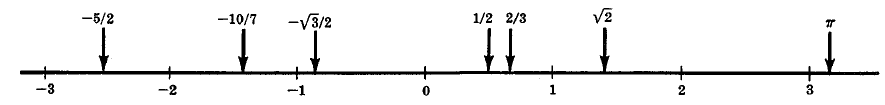
\includegraphics[width=.8\textwidth]{./calculo/fig-01-01--recta_numerica.png}
 % fig-01-01--recta numérica.png: 885x105 px, 120dpi, 18.73x2.22 cm, bb=0 0 531 63
 \label{fig:schaum 01 01}
\end{figure}


%%%%%%%
{Números reales}
	La unión de número racionales e irracionales se le conoce como \emph{números reales} $\R$.

%%%%%%%
\subsection{Orden}

	Los números reales se clasifican en
	\begin{itemize}
		\item Positivos $\set{x\in \R| x>0}$ 
		\item Cero $\set{0\in \R}$ 
		\item Negativos $\set{x\in \R | x<0}$
	\end{itemize}

%%%%%%%

 Diremos que $b\in \R$ es mayor que $a\in\R$ si $b-a>0$. 
  
 
 En ese caso escribimos $b>a$.

%%%%%%%
{}
	Diremos que $a\in \R$ es menor que  $b\in\R$ si $a-b<0$.
	
	En ese caso escribimos $a<b$.

%%%%%%%
{}
	\begin{proposicion}
		\begin{align*}
		b>a \iff a<b	
		\end{align*}
	\end{proposicion}

%%%%%%%
{Desigualdades}
	\begin{proposicion}
		Sean $a,b\in\R$. Entonces se cumple una y solo una de las siguientes condiciones:
		\begin{itemize}
			\item $a>b$
			\item $a=b$
			\item $a<b$
		\end{itemize}
	\end{proposicion}

%%%%%%%
\subsection{Reglas de álgebra}
%\subsection{Axiomas}

	Para cualesquiera $a,b,c\in\R$, se tienen las siguientes propiedades:

%%%%%%%
{}
	\begin{axioma}[Conmutatividad de la suma]
		\label{axiom--1}
		\begin{align*}
		a+b=b+a
		\end{align*}
	\end{axioma}

%%%%%%%
{}
	\begin{axioma}[Asociatividad de la suma]
		\label{axiom--2}
		\begin{align*}
	(a+b)+c = a+(b+c)
		\end{align*}
	\end{axioma}

%%%%%%%
{}
	\begin{axioma}[Conmutatividad del producto]
		\label{axiom--3}
		\begin{align*}
		ab=ba
		\end{align*}
	\end{axioma}

%%%%%%%

{}
	\begin{axioma}[Asociatividad del producto]
		\label{axiom--4}
		\begin{align*}
		(ab)c = a(bc)
		\end{align*}
	\end{axioma}

%%%%%%%
{}
	\begin{axioma}[Ley de la distribución]
		\label{axiom--5}
		\begin{align*}
		a(b+c)=ab+ac
		\end{align*}
	\end{axioma}

%%%%%%%
{Leyes de los exponentes}
	\begin{itemize}
		\item $a^{m}\cdot a^{n} = a^{m+n}$ 
		\item $\dfrac{a^{m}}{a^{n}} = a^{m-m}, a\neq 0$ 
		\item $\left(a^{m}\right)^{n} = a^{mn}$
	\end{itemize}


	\begin{itemize}
		\item $ a^{1}= a $ 
		\item $ a^{0}= 1 $ 
		\item $ a^{-1}= \dfrac{1}{a} $ 
		\item $ a^{n}= \dfrac{1}{a^{n}}  $
		\item $ a^{p/q}= \sqrt[q]{a^{p}} $
	\end{itemize}

\subsection{Ejemplos}

{}
 \begin{problema}
 	Demuestra que $\sqrt{2}$ es un número irracional.
 \end{problema}

%%%%%%%
{Solución}
	Procedamos por contradicción: 
	\begin{enumerate}
		\item Supongamos que $\sqrt{2}=\dfrac{p}{q}$ con $ p,q \in \Z$ positivos y primos relativos.  
		\item Entonces $ 2= \dfrac{p^{2}}{q^{2}}$, de manera que $p^{2}=2q^{2}$.
		\item De manera que $p$ es par, es decir, existe un entero $m$ tal que $p=2m$. 
		\item Sustituyendo obtenemos que $q^{2}=2m^{2},$ de manera que $q$ también es par. 
		\item Pero por hipótesis, $p$ y $q$ son primos relativos, de manera que no pueden ser ambos pares. $\qed$
	\end{enumerate}


%%%%%%%
{}
	\begin{problema}
		¿Qué número es más grande: $\sqrt{2}$ o $ \sqrt[3]{3} $?
	\end{problema}

%%%%%%%
{Solución}
	Procedamos por contradicción:
	\begin{enumerate}
		\item 
		Supongamos que $ \sqrt{2} \geq \sqrt[3]{3}$. 
		\item Elevamos ambos lados a la sexta potencia. 
		\item De donde obtenemos que 
		\begin{align*}
			2^{3} \geq 3^{2} \qed
		\end{align*} 
	\end{enumerate}

%%%%%%%
{}
	\begin{problema}
		Con base en los axiomas \eqref{axiom--1}-\eqref{axiom--5}, demostrar que
		\begin{align*}
			(b+c)a=ba+ca
		\end{align*}
	\end{problema}

%%%%%%%
{Solución}
		\begin{align*}
		(b+c)a &= a(b+c)\\ 
		&=ab+ac \\ 
		&=ba+ca
		\end{align*}


\section{Funciones}

\subsection{Definición}
{}
  Una \emph{función} $f$ es una regla que asigna a cada elemento $x$ de un conjunto $A$ un único elemento $y$ de otro conjunto $B$. 
  
  En ese caso escribiremos $f:A \to B$

%%%%%%%%%%%%%%%%%%%%%
{}
\begin{enumerate}[(i)]
  %NUEVO ITEM
  \item 
  Para indicar dicha correspondencia escribimos $y=f(x)$ y decimos que $y$ es el \emph{valor} de $f$ en $x$. 
  \item Al conjunto $A$ se le conoce como dominio. 
  \item Mientras que al conjunto $B$, se le conoce como contradominio.
\end{enumerate}

%%%%%%%%%%%%%%%%%%%%%
{}
  \begin{problema}
   Evaluar $f(x)=x^{2}-3x+2$ en $x=2$
  \end{problema}

  \begin{proof}[Solución]
     \begin{align} 
	f(2) &= (2)^{2}-3(2)+2 \\
   &=  0
   \end{align}
  \end{proof}

%%%%%%%%%%%%%%%%%%%%%
{}
  \begin{defn}
   La \emph{gráfica} de una función $f: A \to B$ es el conjunto 
       \begin{align}    
   \Gamma_{f} = \sett{\left( a,b \right)\in A\times B}{b=f(a)}
    \end{align}
  \end{defn}


%%%%%%%%%%%%%%%%%%%%%
{}
\begin{enumerate}[(i)]
  %NUEVO ITEM
  \item 
  En el caso $A=B=\R^{n}$, diremos que la gráfica de $F:\R \to \R$ es una \emph{curva}. 
  
  \item Diremos que $x\in A$ es la variable \emph{independiente},  mientras que $y\in B$ es la variable \emph{dependiente}.
\end{enumerate}

%%%%%%%%%%%%%%%%%%%%%
\subsection{Polinomios}
 
     \begin{align}
   f(x) = a_{n}x^{n}+a_{n-1}x^{n-1}+...+a_{0}
   \end{align}
    
   Si $a_{n}\neq 0$, diremos que $n$ es el grado del polinomio y $a_{n}$, su coeficiente líder. 
   
   
   Denotaremos el grado del polinomio $f$ por $\mathrm{grd}(f)$.

%%%%%%%%%%%%%%%%%%%%%
{}
Si $\mathrm{grd}(f)=n$, la ecuación polinomial $f(x)$ tiene exactamente $n$ raíces (posiblemente repetidas).


\begin{problema}
 Como $x^{3}-3x^{2}+3x-1=0$, se puede reescribir como $(x-1)^{3}$,  entonces la ecuación tiene una raíz $x=1$ repetida 3 veces. 
\end{problema}


%%%%%%%%%%%%%%%%%%%%%
{Teorema del Binomio}
  
     \begin{align}
   \left( a+x \right)^{n} = 
   a^{n}+\binom{n}{1}a^{n-1}x+\binom{n}{2}a^{n-2}x^{2}+...+x^{n}
   \end{align}

donde $\binom{n}{k}=\dfrac{n!}{k!\left( n-k \right)!}$

%%%%%%%%%%%%%%%%%%%%%
\subsection{Exponenciales y logaritmos}
{Funciones exponenciales}
     \begin{align}
   \exp_{a}(x) = a^{x}, a> 0
   \end{align}
   

%%%%%%%%%%%%%%%%%%%%%
{Leyes de los exponentes}

        \begin{align}
    \exp_a(m+n) &= 
     \exp_{a}(m)\cdot \exp_{a}(n) \\
     \exp_a(m-n) &=    
     \dfrac{\exp_a(m)}{\exp_a(n)}     \\
     \exp_a(nm) &=      
     \left( \exp_a(m)\right)^{n}  \\       
     \exp_a(0) &=  1 \\     
     \exp_a(1) &=  a     
     \end{align}

%%%%%%%%%%%%%%%%%%%%%
{Logaritmos}
  La función logarítmica $f(x)=\log_{a}(x)$ es la función inversa de $g(x) = \exp_{a}(x)$, 
   es decir 
       \begin{align}
    \forall x \in \R: \log_{a}\left( \exp_{a}(x) \right) = x
    \end{align}
    
         \begin{align}
     \forall x \in \R^{+}: \exp_{a}\left( \log_{a}(x) \right) = x
     \end{align}

%%%%%%%%%%%%%%%%%%%%%
{Leyes de los logaritmos}
     \begin{align}
   \log_{a}(mn)&= \log_{a}(m)\cdot \log_{a}(n) \\
   \log_{a}\left( \dfrac{m}{n} \right)&= \log_{a}(m)-\log_{a}(n) \\ 
   \log_{a}(m^{p}) &= p\log_{a}(m) \\ 
   \log_{a}(1)&= 0\\ 
   \log_{a}(a)&=1
   \end{align}

%%%%%%%%%%%%%%%%%%%%%
{Logaritmo natural}
  En el caso de que la base sea la constante de Euler, es decir $a=e\approx 2.718$, entonces reescribimos
     \begin{align}
   \exp_{e}(x)=\exp(x)\\ 
   \log_{e}(x)=\ln(x)
   \end{align}
   
   Esta última función se conoce como \emph{logaritmo natural}.

%%%%%%%%%%%%%%%%%%%%%
\subsection{Funciones trigonométricas}
{Relaciones fundamentales}
\begin{align}
\sin(x) &=\cos\left( \dfrac{\pi}{2}-x \right) \\    
\cos(x) &= \sin\left( \dfrac{\pi}{2}-x \right) \\    
\tan(x) &= \dfrac{\sin(x)}{\cos(x)} \\     
\cot(x) &= \dfrac{\cos(x)}{\sin(x)}=\dfrac{1}{\tan(x)} \\    
\sec(x) &= \dfrac{1}{\cos(x)} \\    
\csc(x) &= \dfrac{1}{\sin(x)}
\end{align}

%%%%%%%%%%%%%%%%%%%%%
\subsection{Identidades pitagóricas}
\begin{align}
\sin^{2}(x)+\cos^{2}(x)&= 1\\ 
\sec^{2}(x)-\tan^{2}(x)&= 1\\ 
\csc^{2}(x)-\cot^{2}(x)&= 1
\end{align}

%%%%%%%%%%%%%%%%%%%%%
{Paridad}
     \begin{align}
   \sin(-x) &= -\sin(x) \\ 
   \cos(-x) &= \cos(x) \\ 
   \tan(-x) &= -\tan(x) 
   \end{align}

%%%%%%%%%%%%%%%%%%%%%
{Sumas de ángulos}
     \begin{align}
   \sin(x\pm y) &= \sin(x)\cos(y)\pm\cos(x)\sin(y) \\   
   \cos(x\pm y) &= \cos(x)\cos(y)\mp\sin(x)\sin(y) \\   
   \tan(x\pm y) &= \dfrac{\tan(x)\pm \tan(y)}{1+\mp \tan(x)\tan(y)}
   \end{align}

%%%%%%%%%%%%%%%%%%%%%
{Ondas sinusoidales}
     \begin{align}
   \begin{cases}
A\cos(x)+B\sin(x) = \sqrt{A^{2}+B^{2}}\sin(x+\alpha)\\
\tan(\alpha) = \dfrac{A}{B}
\end{cases}
   \end{align}

%%%%%%%%%%%%%%%%%%%%%
{Periodicidad}
  Las funciones $\sin(x)$ y $\cos(x)$ tiene periodo $T=2\pi$.   
  Mientras que la función $\tan(x)$ tiene periodo $T=\pi$.
  
  
%%%%%%%%%%%%%%%%%%%%%
{Inversas trigonométricas}
   Las funciones inversas de funciones trigonométricas estás sólo definidas \emph{localmente}:  Por ejemplo,
      \begin{align}
     y = \sin(x) \iff x =\sin^{-1}(y)
     \end{align} 
     siempre y cuando 
          \begin{align}
      x\in\left[-\dfrac{\pi}{2}, \frac{\pi}{2} \right],
      y\in\left[ -1,1 \right]
      \end{align}

%%%%%%%%%%%%%%%%%%%%%
\subsection{Funciones hiperbólicas}
{Relaciones fundamentales}
 \begin{align}
\sinh(x) &= \dfrac{e^{x}-e^{-x}}{2}\\ 
\cosh(x) &= \dfrac{e^{x}+e^{-x}}{2}
\end{align}

%%%%%%%%%%%%%%%%%%%%%
{}
\begin{align}
\tanh(x) &= \dfrac{\sinh(x)}{\cosh(x)}\\ 
&=\dfrac{e^{x}-e^{-x}}{e^{x}+e^{-x}}
 \end{align}  

%%%%%%%%%%%%%%%%%%%%%
{}
\begin{align}
\coth(x) &= \dfrac{\cosh(x)}{\sinh(x)}\\ 
& = \dfrac{1}{\tanh(x)}\\ 
& = \dfrac{e^{x}+e^{-x}}{e^{x}-e^{-x}} 
\end{align}

%%%%%%%%%%%%%%%%%%%%%
{}
 \begin{align}
\sech(x)&= \dfrac{1}{\cosh(x)} \\ 
&= \dfrac{2}{e^{x}+e^{-x}}
\end{align}

%%%%%%%%%%%%%%%%%%%%%
{}
\begin{align}
\csch(x)&= \dfrac{1}{\sinh(x)} \\ 
&= \dfrac{2}{e^{x}-e^{-x}}
\end{align}

%%%%%%%%%%%%%%%%%%%%%
{Identidades pitagóricas}
\begin{align}
\cosh^{2}(x)-\sinh^{2}(x)&= 1\\
\sech^{2}(x)+\tanh^{2}(x)&= 1\\
\coth^{2}(x)-\csch^{2}(x)&= 1
\end{align}

%%%%%%%%%%%%%%%%%%%%%
{Sumas de ángulos}
 \begin{align}
\sinh(x\pm y) &= \sinh(x)\cosh(y)\pm \cosh(x)\sinh(y)\\
\cosh(x\pm y) &= \cosh(x)\cosh(y)\pm \sinh(x)\sinh(y)\\
\tanh(x\pm y) &= \dfrac{\tanh(x)\pm \tanh(y)}{1\pm \tanh(x)\tanh(y)}
\end{align}

%%%%%%%%%%%%%%%%%%%%%
\subsection{Ejemplos}
{}
\begin{problema}
\label{solved 1.4}
Si $f(x)=2x^{2}-3x+5$, encontrar
\begin{enumerate}[(i)]
 %NUEVO ITEM     
 \item $f(h)-f(0)$
 
 \item $f(h-1)-f(-1)$
 
 \item $f(x+h)$
 
 \item $f(x+h)-f(x)$
 
 \item $\dfrac{f(x+h)-f(x)}{h}$
\end{enumerate}
\end{problema}


%%%%%%%%%%%%%%%%%%%%%
{}
  \begin{problema}
   \label{solved 1.5}
   Usando las leyes de los exponentes, demostrar las leyes de los logaritmos.
  \end{problema}


%%%%%%%%%%%%%%%%%%%%%
{}
  \begin{problema}
   \label{solved 1.6}
   Demostrar que 
   \begin{enumerate}[(i)]
     %NUEVO ITEM
     \item $\sin^{2}(x)=\dfrac{1}{2}\left( 1-\cos(2x) \right)$ 
     
     \item $\cos^{2}(x)=\dfrac{1}{2}\left( 1+\cos(2x) \right)$
\end{enumerate}
  \end{problema}


%%%%%%%%%%%%%%%%%%%%%
{}
  \begin{problema}
   \label{solved 1.7}
   Demostrar que \[A \cos(x) + B\sin(x) = \sqrt{A^{2}+B^{2}}\sin(x+\alpha)\] donde $\tan(\alpha)=\dfrac{A}{B}$.
  \end{problema}


%%%%%%%%%%%%%%%%%%%%%
{}
  \begin{problema}
   \label{solved 1.8}
   Demostrar que 
   \begin{enumerate}[(i)]
     %NUEVO ITEM
     \item $\cosh^{2}(x)-\sinh^{2}(x)=1$       
     \item $\sech^{2}(x)+\tanh^{2}(x)=1$
\end{enumerate}
  \end{problema}


%%%%%%%%%%%%%%%%%%%%%
{}
  \begin{problema}
   \label{solved 1.9}
   Demostrar que $\cosh^{-1}(x)=\pm \ln\left( x+\sqrt{x^{2}-1} \right)$
  \end{problema}


%%%%%%%%%%%%%%%%%%%%%

\section{Números complejos}

En estas notas, denotaremos por $\R$ el conjunto de números reales. En esta sección, procederemos de manera informal,
para motivar la definición de un número complejo y formalizar sus propiedades, en secciones posteriores. 


Supongamos que $a,b,c\in \R,$ y queremos resolver
la ecuación
$$
ax^2+bx+c=0.
$$

De manera algebraíca encontramos que las soluciones estan dadas por la fórmula
$$
x=\dfrac{-b\pm \sqrt{D}}{2a}, \, D=b^2-4ac.
$$

Si $D \geq 0,$ entonces $D$ es un número real. Sin embargo, ¿qué sucede si $D<0$?. Por la \emph{ley de los signos} si
$x,y\geq 0,$ entonces $xy\geq 0.$ De la misma manera, si $x,y<0,$ entonces $xy>0.$ En particular, para cualquier
$x\in \R,$ tenemos que $x^{2}=x\cdot x\geq 0.$ Por lo tanto, $\sqrt{D} \notin \R$ si $D<0.$

Una solución a este problema es definir el número $i=\sqrt{-1}.$ En este caso, si $D<0,$ entonces usando leyes de los
exponentes tenemos que
$$
\sqrt{D}=\sqrt{(-1)(-D)}=\sqrt{-1}\sqrt{-D}=\sqrt{-D}i.
$$
En este caso, como $D<0,$ entonces $-D>0$ y $\sqrt{-D}\in \R.$

\begin{problema}
 Las soluciones de la ecuación $x^2+1=0$ son $x=0+i1$ y $x=0+i(-1),$ o simplemente, $x=\pm i.$
\end{problema}

\begin{problema}
 Encuentre las soluciones de la siguientes ecuaciones:
 \begin{enumerate}
  \item $x^{4}+16=0,$
  \item $x^{2}-2x+2=0.$
 \end{enumerate}

\end{problema}


 Entonces, diremos que un número complejo es una cantidad de la forma
 $$
z=x+iy, \, x,y\in \R, \, i=\sqrt{-1}.
 $$
 Observe que si $x\in \R,$ podemos identificarlo con $x+i0.$

Definimos la suma de números complejos $z=x+iy,z'=x+iy'$ de la siguiente manera:
$$
z+z'=(x+x')+i(y+y').
$$

\begin{problema}
Demuestre que 
\begin{enumerate}
 \item $(x+iy)+(x'+iy')=(x'+iy')+(x+iy).$
 \item $\left[ (x+iy)+(x'+iy') \right] +(x''+iy'')= (x+iy)+\left[ (x'+iy') +(x''+iy'') \right]$
 \item $0+(x+iy)=x+iy$
 \item $(x+iy)+((-x)+i(-y))=0$
\end{enumerate}\end{problema}

Diremos que $0=0+i0$ es el \emph{neutro aditivo} en los número complejos y que $-z:=-x-iy$ es el \emph{inverso aditivo}
de $z=x+iy.$

Ahora queremos definir la multiplicación $(x+iy)(x'+iy').$ Sigamos las reglas algebraicas usuales para números reales,
salvo por la identidad $i^2=-1.$

\begin{align*}
(x+iy)(x'+iy')&= x(x'+iy')+iy(x'+iy')\\
&= xx'+x(iy')+(iy)x'+(iy)(iy') \\
&= xx' + ixy +iyx' + i^{2}yy' \\
&= (xx'-yy')+i(xy'+yx').
\end{align*}

En resumen,
 $$
zz'= (xx'-yy')+i(xy'+yx') \in \C.
 $$

\begin{problema}
Demostrar las siguientes propiedades de la multiplicación de número complejos
\begin{enumerate}
 \item $(x+iy)(x'+iy')=(x'+iy')(x+iy).$
 \item $\left[ (x+iy)(x'+iy') \right] (x''+iy'')= (x+iy)\left[ (x'+iy') (x''+iy'') \right]$
 \item $(1+i0)(x+iy)=x+iy$
 \item $(x+iy)(x-iy)=x^2+y^2.$
 \item $(x+iy)\left( \dfrac{x-iy}{x^2+y^2} \right)=1.$
\end{enumerate}
\end{problema}

Diremos que $1=1+i0$ es el \emph{neutro multiplicativo} en los número complejos y que $$
z^{-1}:=\dfrac{x-iy}{x^2+y^2} 
$$ es el \emph{inverso multiplicativo} de $z=x+iy.$

Si definimos $\bar{z}=x-iy,$ para $z=x+iy,$ podemos reescribir $$z^{-1}=\dfrac{\bar{z}}{z\bar{z}}.$$
Diremos que $\bar{z}$ es el \emph{conjugado} de $z.$

\begin{observacion}
Los número reales se pueden identificar con una línea recta. Como $i$ no se puede identificar con un número en la línea
recta, se decía que este número era \emph{imaginario.} Sin embargo, podemos visualizar los números complejos (es decir,
¡dibujarlos!), para lo cuál necesitaremos ``más espacio''. Como requerimos dos números reales para describir un
complejo, tendremos que dibujarlos en el plano.
\end{observacion}

\begin{problema}
\label{exe:1.1.1}
 Encuentre el resultado de las siguientes operaciones:
 \begin{enumerate}
  \item $\left( 1+i\sqrt{3} \right)\left( -1 +i\sqrt{3} \right)$
  \item $\dfrac{\frac{1}{\sqrt{2}}+i\frac{1}{\sqrt{2}}}{\sqrt{3}+i1}$
  \item $\left( \sqrt{2}+i\sqrt{6} \right)^{3}$
 \end{enumerate}

\end{problema}

\subsection{Estructura algebraica de $\C$}

\begin{definicion}El \emph{plano} es el conjunto
	$$
	\R^{2}=\set{(x,y)|x,y\in \R },
	$$
	de parejas ordenadas de números reales.
\end{definicion}

En este espacio, podemos definir varias operaciones. Cuando al conjunto lo dotamos de ciertas operaciones, decimos que
es un \emph{estructura (matemática)} en el plano. Una de las más importantes es la estructura de \emph{espacio
	vectorial,} que a continuación presentamos.

\begin{definicion} El \emph{plano euclideano} es $\R^{2}$ dotado de las siguiente operaciones:
	\begin{enumerate}
		\item 
		$
		(x,y)+(x',y')=(x+x',y+y'),
		$
		\item Si $\a \in \R,$
		$
		\a\cdot(x,y)=(\a x,\a y),
		$
	\end{enumerate}
\end{definicion}

\begin{observacion}
	En este caso, a los pares ordenados $(x,y)\in \R^{2}$ les llamaremos \emph{vectores (en el plano)}, mientras que a los
	números reales los llamaremos \emph{escalares.} Entonces, nos referiremos a la primera operación como \emph{suma de
		vectores,} mientras que a la segunda como \emph{multiplicación por escalares.} Estas son las operaciones \emph{usuales}
	en el plano euclideano.
\end{observacion}


\begin{problema}
	Encuentre y grafique los vectores resultantes.
	\begin{enumerate}
		\item $2(1,0)+3(0,1),$
		\item $\frac{1}{5}(5,0)-1(0,2).$
	\end{enumerate}
	
\end{problema}

Con el plano euclideano en mente, podemos definir de manera formal el conjunto de número complejos. Observe que
podríamos identificar $x+iy$ con el vector $(x,y).$ Observe que con esta identificación, el resultado de la suma de
números complejos coincide con la de vectores. De igual manera, podemos identificar la multiplicación entre número
complejo. Esto nos lleva a la definición formal de \emph{números complejos.}

\begin{definicion}
	El \emph{campo} de número complejos $\C$ es el conjunto $\R^{2}$ dotado de las siguientes operaciones:
	\begin{enumerate}
		\item
		$
		(x,y)+(x',y')=(x+x',y+y'),
		$
		\item
		$
		(x,y)(x',y')=(xx'-yy',xy'+yx').
		$
	\end{enumerate}
\end{definicion}


Si identificamos $\a \in \R,$ con $(a,0) \in \C,$ resulta que la multiplicación por escalares coindice con la
multiplicación de números complejos para escalares reales, es decir, si $a\in \R,$
$$
a(x,y)=(a,0)(x,y).
$$

\begin{problema}
	Verifique la afirmación anterior.
\end{problema}


\begin{problema}
	Verifque las siguiente propiedades. Si $u,v,w \in \C \cong \R^{2},$ entonces
	\begin{enumerate}
		\item $u+v\in \C$ 
		\item $(u+v)+w=u+(v+w)$
		\item $u+v=v+u$
		\item Existe $0\in \C,$ tal que $u+0=0$
		\item Para cada $u\in \C,$ existe $-u\in\C,$ tal que $u+(-u)=0$
		\item $uv \in \C$
		\item $(uv)w=u(vw)$
		\item $uv=vu$
		\item Existe $1\in \C,$ tal que $1u=u$
		\item Para cada $u\in C, u \neq 0,$ existe $u^{-1}\in \C,$ tal que $u u^{-1}=1$
		\item $u(v+w)=uv+uw.$
	\end{enumerate}
	
\end{problema}

\begin{observacion}
	Cualquier conjunto $S,$ con operaciones suma y multiplicación, que cumplan las propiedades anteriores, se conoce como
	un \emph{campo.} Otros ejemplos de campos son las fracciones y los mismos números reales. En teoría número, ejemplos de
	campos son los enteros \emph{módulo} $p$ $\mathbb{Z}_{p},$ con $p$ un número primo.
\end{observacion}

\subsection{Forma polar de los números complejos}

En la presente sección, suponemos que el lector tiene conocimientos elementales de trigonometría y geometría analítica. 

Como los números complejos son vectores, podemos calculas su longitud o \emph{norma.}

\begin{definicion}
	Si $z=x+iy\in \C,$ entonces la norma de $z$ se define como
	$$
	\norm{z}=\sqrt{x^{2}+y^{2}}.
	$$
\end{definicion}

Como hicimos antes, definimos de manera formal el \emph{conjugado} de un número complejo.
\begin{definicion}
	Si $z=(x,y)\in \C,$ su \emph{conjugado} esta dado por
	$$
	\bar{z}=(x,-y)\in \C.
	$$
\end{definicion}

De manera que $\norm{z}^{2}=z\bar{z}.$

De la misma manera, siendo un vector podemos medir el ángulo que abre respecto al vector $(1,0)$, en el sentido de las
manecillas del reloj, al cual llamaremos \emph{argumento} y definimos analíticamente de la siguiente forma.
\begin{definicion}
	El argumento $\theta(z)$ de $z=x+iy\in \C$ se define como
	\begin{enumerate}
		\item $\arctan\left( \dfrac{y}{x} \right)$ si $x>0$
		\item $\pi + \arctan\left( \dfrac{y}{x} \right)$ si $x<0$
		\item $\dfrac{\pi}{2}$ si $x=0, y> 0$
		\item $-\dfrac{\pi}{2}$ si $x=0, y< 0$
	\end{enumerate}
	
\end{definicion}

\begin{definicion}
	Si $z\in \C$ tiene norma $r>0$ y argumento $\th,$ decimos que $$
	z=r\arg{\th},
	$$
	es la \emph{forma polar} de $z,$ donde $\arg{\cdot}:\R\to\R^{2},$
	$$
	\arg{\th}=\, \left( \cos(\th), \sin (\th) \right).
	$$
\end{definicion}

\begin{problema}
	Demostrar que
	\begin{enumerate}
		\item $\arg{0}=1$
		\item $\arg{\th+2\pi}=\arg{\th}$
		\item $\overline{\arg{\th}}=\arg{-\th}$
		\item $\arg{\th+\tau}=\arg{\th}\arg{\tau}$
		\item $\arg{n\th}=\left( \arg{\th} \right)^{n}$
	\end{enumerate}
	
\end{problema}

\begin{problema}
	\begin{enumerate}
		\item Si $z=r\arg{\th} \in \C,$ entonces
		\begin{enumerate}
			\item   $
			z^{-1}=r^{-1} \overline{\arg{\th}}
			$
			\item Si $n$ es un número entero, $
			z^{n}=r^{n}\arg{n \th}.
			$
		\end{enumerate}
		
		
		\item Si $z=r\arg{\th}, w=s\arg{\tau} \in \C,$ entonces
		\begin{enumerate}
			\item   $
			zw=rs\arg{\th+\tau}.
			$
			\item
			$
			\dfrac{z}{w}=\dfrac{r}{s}\arg{\th-\tau}
			$
		\end{enumerate}
		
		
		
		
		
	\end{enumerate}
	
\end{problema}

Esta última identidad se conoce como \emph{identidad de De Moivre.}


\begin{problema}
	Convierta a su forma polar, cada uno de los números en el ejercicio \ref{exe:1.1.1} y realice las operaciones
	correspondientes, usando los resultados anteriores. 
\end{problema}




\chapter{Álgebra}


%201
\section{Reducci\'on de t\'erminos semejantes}

 En el álgebra, representamos cantidades desconocidas por s\'imbolos;  generalmente son letras como $x,y,z,$ pero \emph{no debe olvidarse que respresentan números.}



	Para representar una multiplicaci\'on iterada, usamos el s\'imbolo de potencia
	$$
	x^{n}=\underbrace{x\cdot\cdots \cdot x}_{n\texttt{-veces}};
	$$
	al número $x$ le llamamos base y al número $n$ le llamamos potencia.



	\begin{problema}
		\begin{enumerate}
			\item $3^{2}=3\cdot3=9$
			\item $5^{3}=5\cdot5\cdot5=125$
			\item $2^{4}=2\cdot2\cdot2\cdot2=16$
		\end{enumerate}
		
	\end{problema}
	



	\begin{problema}
		\begin{enumerate}
			\item $x^{2}=x\cdot x$
			\item $x^{3}=x\cdot x\cdot x$
			\item $x^{4}=x\cdot x\cdot x\cdot x$
			\item $\cdots$
		\end{enumerate}
		
	\end{problema}




	\begin{rem}
		Observe que $x^{1}=x;$ mientras que, por convenci\'on, $x^{0}=1.$
	\end{rem}
	



	Cuando multiplicamos $x^{n}$ por un número diferente de $x:$
	$$ax^{n}=a\cdot\underbrace{x\cdot\cdots *x},$$ diremos que $a$ es el coeficiente de $x^{n}.$ 



	A un número escrito en la forma $ax^{n}$ se le llama \emph{monomio;} y diremos que dos monomios son semejantes si tienen \emph{exactamente} la misma base a la misma potencia.



	\begin{problema}
		Determine cual de los siguientes monomios es semejante a $2x^{3}:$
		\begin{enumerate}
			\item $3x^{3};$
			\item $2x^{2};$
			\item $2y^{3};$
		\end{enumerate}
		
	\end{problema}
	



	Dos t\'erminos semejantes pueden reducirse 
	$$\begin{cases}
		ax^{n}+bx^{n}=\left( a+b \right)x^{n}\\
		ax^{n}-bx^{n}=\left( a-b \right)x^{n}
	\end{cases}
	$$



	\begin{problema}
		Reduzca los siguientes t\'erminos semejantes, escribiendo el coeficiente en forma irreducible.
		\begin{enumerate}
			\item $\left( 4n^{2}+5n+3 \right)+\left( -3n^{2}-2n \right)$
			\item $\left( -7a^{3}-a^{2}-5a-2 \right)+\left( a^{3}+a^{2}-4a+7 \right)$
			\item \begin{eqnarray*}
				\left(5u^{5}-3u^{4}+2u^{3}-5u^{2}+7u-7\right)+ \\
				\left( \dfrac{2u^{5}}{3}+\dfrac{3u^{4}}{2}-\dfrac{2u^{2}}{3}+\dfrac{5u}{6}+\dfrac{5}{4} \right).
			\end{eqnarray*}
			
		\end{enumerate}
		
	\end{problema}
	



	\begin{problema}
		Reduzca los siguientes t\'erminos semejantes, escribiendo el coeficiente en forma irreducible.
		\begin{enumerate}
			\item $\left( 4n^{2}+5n+3 \right)-\left( -3n^{2}-2n \right)$
			\item $\left( -7a^{3}-a^{2}-5a-2 \right)-\left( a^{3}+a^{2}-4a+7 \right)$
			\item \begin{eqnarray*}
				\left(5u^{5}-3u^{4}+2u^{3}-5u^{2}+7u-7\right)- \\
				\left( \dfrac{2u^{5}}{3}+\dfrac{3u^{4}}{2}-\dfrac{2u^{2}}{3}+\dfrac{5u}{6}+\dfrac{5}{4} \right).
			\end{eqnarray*}
			
		\end{enumerate}
		
	\end{problema}
	



	\begin{rem}
		A la suma de dos o más monomios se le conoce como \emph{polinomio}.
		
		Por ejemplo $x^{2}-2x+1$ o $x^{2}-2xy+y^{2}.$
		
	\end{rem}
	



%202
\section{Supresi\'on de signos de agrupaci\'on}


	Cuando queremos quitar parentesis u otro signo de agrupaci\'on, en una suma o resta de polinomios, basta usar la regla de los signos.



	Sin embargo, cuando un polinomio se multiplica por un coeficiente, se utiliza la siguiente regla
	\begin{prop}[Ley de la distribuci\'on]
		\begin{eqnarray}
			\label{distribucion}
			a\left( b+c \right)=ab+ac\\
			\left( a+b \right)\left( c+d \right)=ac+ad+bc+bd.
		\end{eqnarray}
		
	\end{prop}
	



	\begin{problema} Simplifique
		\begin{enumerate}
			\item $(6-7a)(2-4a)$
			\item $-4(-4w-5)(4w-2)$
			\item $6(-5v-7)(4-5v)(-2v-1)v$
		\end{enumerate}	
	\end{problema}
	



%203
\section{Mutiplicaci\'on de polinomios}


	Dos monomios se pueden multiplicar de la siguiente manera
	$$
	(ax^{n})(bx^{m})=(ab)x^{n+m}.
	$$



	\begin{problema}
		\begin{enumerate}
			\item $\left( 2x^{3} \right)\left( 3x^{2} \right)=\left( 2*3 \right)x^{2+3}=6x^{5}.$
		\end{enumerate}
		
	\end{problema}
	



	\begin{problema}
		Exprese su respuesta en la forma más simple posible:
		\begin{enumerate}
			\item $(6x^{4})(4-3x-3x^{2})$
			\item $5w^{3}\left( -7w^{3}-7w^{2}+7w+3 \right)$
			\item $\dfrac{a^{3}}{3}\left( -7a^{5}-2a^{4}+3a^{3}+a^{2}-a-3 \right)$
		\end{enumerate}
		
	\end{problema}
	



	\begin{problema}
		Exprese su respuesta en la forma más simple posible:
		\begin{enumerate}
			\item $$
			\left( n^{2}+5n \right)
			\left( -n^{2}+6n+1 \right)
			$$
			
			\item $$
			\left( -6a^{2}-3a-7 \right)
			\left( a^{3}+a^{2}+6a-7 \right)
			$$
			
			\item $$
			\left( \dfrac{9w^{4}}{8}+\dfrac{8w^{3}}{9}-\dfrac{7w^{2}}{9}-\dfrac{w}{3}+\dfrac{5}{9} \right)
			\left( -2w^{3}-5w+7 \right)
			$$
		\end{enumerate}
		
	\end{problema}
	



	\begin{problema}
		Exprese su respuesta en la forma más simple posible:
		\begin{enumerate}
			\item $(7u^4)\left( 6-4u-7u^{2} \right)$ 
			\item $(3s^{4})\left( -7+s-s^{2}-5s^{3} \right)$
			\item $(7x^{4})\left( 2+4x-7x^{2} \right)$
		\end{enumerate}
	\end{problema}



	\begin{problema}
		Simplifique
		\begin{enumerate}
			\item $(5w^{4})\left( -1+5w+4w^{2}+6w^{3} \right)$
			\item $(3m^{4})\left( -1-6m-3m^{2}-7m^{3}-4m^{4} \right)$
			\item $5a^{5}\left( a^{3}-3a^{2}+3a-5 \right)$
		\end{enumerate}
		
	\end{problema}
	
	



	\begin{problema}
		Escriba su respuesta de la forma más simple posible
		\begin{enumerate}
			\item $\left( \dfrac{8n^{4}}{9} \right)\left( n^{4}-3n^{3}-4n^{2}+3n-1 \right)$
			\item $\left( \dfrac{2y^{5}}{5} \right)\left( -3y^{4}+5y^{3}-7y^{2}-2y-5 \right)$
			\item $\left( \dfrac{3s^{3}}{7} \right)\left( -2s^{4}-s^{3}-5s^{2}+2s+1 \right)$
		\end{enumerate}
		
	\end{problema}
	



	\begin{problema}
		Exprese su respuesta en la forma más simple posible
		\begin{enumerate}
			\item $\left( -4x-5 \right)\left( -3x^{3}+3x^{2}-4x-4 \right)$
			\item $\left( 6y-7y^{2} \right)\left( y+3 \right)$
			\item $\left( \dfrac{7w^{2}}{9}+\dfrac{4w}{9}+\dfrac{9}{2} \right)\left( 5w^{2}+6w-7 \right)$
		\end{enumerate}
		
	\end{problema}
	



	\begin{problema}
		Simplifique
		\begin{enumerate}
			\item $\left( 3x^{2}+2x+3 \right)\left( 6x^{2}-4x-3 \right)$
			\item $\left( 4m^{2}+3m \right)\left( 6m^{3}+6m^{2}-7m+6 \right)$
			\item $\left( -4x^{2}+5x+5 \right)\left( 3-4x \right)$
			
		\end{enumerate}
		
	\end{problema}
	



	\begin{problema}
		Simplifique
		\begin{enumerate}
			\item $\left( -2s^{4}-5s^{3}+3s^{2}+3s+2 \right)\left( 7s^{3}-3s^{2}-2s-7 \right)$
			\item $\left( 5v-v^{2} \right)\left( 2v^{2}+6v+5 \right)$
			\item $\left( 7x^{3}+2x^{2}+5x-6 \right)\left( 6x^{3}+3x^{2}-4x-4 \right)$
		\end{enumerate}
		
	\end{problema}
	



	\begin{problema}
		Simplifique
		$$
		\left( \dfrac{2a^{3}}{5}-\dfrac{5a^{2}}{6}-\dfrac{9a}{8}+\dfrac{2}{3} \right)\left( 3a^{2}-2a-4 \right)
		$$
	\end{problema}
	

% 
% \section{División de Polinomios}
% 
% 
%  \begin{problema}
%  \label{st:3.2.1}
%   Divida $6x^{2}-26x+12$ entre $x-4.$ Compruebe.
%  \end{problema}
% 
% 
% 
% 
%  \begin{proof}[Soluci\'on]
%   $$6x^{2}-26x+12=\left( x-4 \right)\left( 6x-2 \right)+4$$
%  \end{proof}
% 
% 
% 
% 
%  \begin{problema}
%  \label{st:3.2.2}
%   Divida $8x^{4}+6x^{2}-3x+1$ entre $2x^{2}-x+2.$ Compruebe
%  \end{problema}
% 
% 
% 
% 
%  \begin{proof}[Sol.]
%   $$
%   8x^{4}+6x^{2}-3x+1=
%   \left( 2x^{2}-x+2 \right)
%   \left( 4x^{2}+2x \right)+
%   \left( -7x+1 \right)
%   $$
%  \end{proof}
% 
% 
% 
% 
%  \begin{problema}
%   Divida $2x^{3}-7x^{2}+5$ entre $x-3.$ Repita el ejericicio \emph{usando divisi\'on sint\'etica.} Compruebe.
%  \end{problema}
% 
% 
% 
% 
%  \begin{proof}[Sol.]
%   $$2x^{3}-7x^{2}+5=
%   \left( x-3 \right)
%   \left( 2x^{2}-x-3 \right)-4$$
%  \end{proof}
% 
% 
% 
% 
%  \begin{problema}
%   Realice las siguientes divisiones; comprebe.
%   \begin{enumerate}
%    \item $\dfrac{x^{2}-6x-8}{x-4}$
%    \item $\dfrac{4x^{3}+2x^{2}-2x-3}{2x+1}$
%    \item $\dfrac{x^{3}+6x+3}{x^{2}-2x+2}$
%    \item $\dfrac{6x^{3}+2x^{2}+22x}{2x^{2}+5}$
%    \item $\dfrac{x^{6}+x^{4}+x^{2}+1}{x^{2}+1}$
%   \end{enumerate}
% 
%  \end{problema}
% 
% 
% 
% 
%  \begin{problema}
%   Realice las siguientes operaciones, \emph{utilizando divisi\'on sint\'etica.} Compruebe.
%   \begin{enumerate}
%    \item $\dfrac{x^{2}-5x+4}{x-3}$
%    \item $\dfrac{3x^{2}+5x}{x-6}$
%    \item $\dfrac{x^{3}+2x^{2}+2x+1}{x+2}$
%    \item $\dfrac{x^{3}-8x+2}{x+3}$
%    \item $\dfrac{x^{5}+3x^{3}-6}{x-1}$
%   \end{enumerate}
% 
%  \end{problema}
% 
% 

%%\section{Productos Especiales}

%204
\section{Productos notables}


	A continuaci\'on, aparecen algunos de los productos que se presentan con frecuencia en matemáticas.


{Producto monomio-binomio}
	\begin{equation}
		a(c+d)=ac+ad
	\end{equation}	



	\begin{problema}
		\begin{enumerate}
			\item $2xy\left( 3x^{2}y - 4y^{3}\right)$ 
			\item $3x^{2}y^{3}\left( 2xy-x-2y \right)$ 
			\item $\left( 2st^{3}-4rs^{2}+3s^{3}t \right)
			\left( 5rst^{2} \right)$
		\end{enumerate}
		
	\end{problema}
	



{Diferencia de cuadrados}
	\begin{equation}
		\left( a+b \right)\left( a-b \right)
		=a^{2}-b^{2}
	\end{equation}
	



	\begin{problema}
		\begin{enumerate}
			\item $\left( 3a+5b \right)\left( 3a-5b \right)$ 
			\item $\left( 5xy+4 \right)\left( 5xy-4 \right)$ 
			\item $\left( 2-5y^{2} \right)\left( 2+5y^{2} \right)$ 
			\item $\left( 3a+5a^{2}b \right)\left( 3a-5a^{2}b \right)$
		\end{enumerate}
		
	\end{problema}
	



{Cuadrado de un binomio}
	\begin{align}
		\left( a+b \right)^{2}&=
		a^{2}+2ab+b^{2}\\
		\left( a-b \right)^{2}&=
		a^{2}-2ab+b^{2}
	\end{align}
	



	\begin{problema}
		\begin{enumerate}
			\item $\left( x+6 \right)^{2}$ 
			\item $\left( y+3x \right)^{2}$ 
			\item $\left( z-4 \right)^{2}$ 
			\item $\left( 3-2x^{2} \right)^{2}$  
			\item $\left( x^{2}y-2z \right)^{2}$ 
		\end{enumerate}
		
	\end{problema}
	



{Producto de dos binomios}
	\begin{align}
		\left( x+a \right)\left( x+b \right)&=
		x^{2}+\left( a+b \right)x+ab\\
		\left( ax+b \right)\left( cx+d \right)&=
		acx^{2}+\left( ad+bc \right)x+bd
	\end{align}
	



	\begin{problema}
		\begin{enumerate}
			\item $\left( x+2 \right)\left( x+4 \right)$ 
			\item $\left( x-4 \right)\left( x+7 \right)$ 
			\item $\left( y+3 \right)\left( y-5 \right)$ 
			\item $\left( xy+6 \right)\left( xy-4 \right)$ 
			\item $\left( 2x-3 \right)\left( 4x+1 \right)$ 
			\item $\left( 4+3r \right)\left( 2-r \right)$
		\end{enumerate}
		
	\end{problema}
	



{Cubo de un binomio}
	\begin{align*}
		\left( a+b \right)^{3}&=
		a^{3}+3a^{2}b+3ab^{2}+b^{3}\\
		\left( a-b \right)^{3}&=
		a^{3}-3a^{2}b+3ab^{2}-b^{3}
	\end{align*}
	



	\begin{problema}
		\begin{enumerate}
			\item $\left( 2x+1 \right)^{3}$ 
			\item $\left( 3x+2y \right)^{3}$ 
			\item $\left( r-2s \right)^{3}$ 
			\item $\left( x^{2}-1 \right)^{3}$ 
			\item $\left( ab^{2}-2b \right)^{3}$
		\end{enumerate}
		
	\end{problema}
	



{Cuadrado de un trinomio}
	\begin{equation}
		\left( a+b+c \right)^{2}=
		a^{2}+b^{2}+c^{2}+2ab+2ac+2bc.
	\end{equation}
	



	\begin{problema}
		$$
		\left( x-2y+z \right)^{2}. 
		$$
	\end{problema}
	



%205
\section{Sumas y diferencias de potencias}


	\begin{problema}
		\begin{align*}
			\left( a-b \right)\left( a^{2}+ab+b^{2} \right)\\
			\left( a-b \right)\left( a^{3}+a^{2}b+ab^{2}+b^{3} \right)\\
			\left( a-b \right)\left( a^{4}+a^{3}b+a^{2}b^{2}+ab^{3}+b^{4} \right)
		\end{align*}
		
	\end{problema}
	



	\begin{problema}
		\begin{align*}
			\left( a+b \right)\left( a^{2}+ab+b^{2} \right)\\
			\left( a+b \right)\left( a^{3}+a^{2}b+ab^{2}+b^{3} \right)\\
			\left( a+b \right)\left( a^{4}+a^{3}b+a^{2}b^{2}+ab^{3}+b^{4} \right)
		\end{align*}
		
	\end{problema}
	



	\begin{problema}
		\begin{enumerate}
			\item $\left( t-2 \right)\left( t^{2}+2t+4 \right)$ 
			\item $\left( z-x \right)\left( x^{2}+xz+z^{2} \right)$ 
			\item $\left( x+3y \right)\left( x^{2}-3xy+9y^{3} \right)$
		\end{enumerate}
		
	\end{problema}
	



	\begin{problema}
		\begin{enumerate}
			\item $\left( s-1 \right)\left( s^{3}+s^{2}+s +1\right)$ 
			\item $\left( 1+t^{2} \right)\left( 1-t^{2}+t^{4}-t^{6} \right)$ 
			\item $\left( 3x+2y \right)^{2}\left( 3x-2y \right)^{2}$ 
			\item $\left( x^{2}+2x+1 \right)^{2}\left( x^{2}-2x+1 \right)^{2}$ 
			\item $\left( y-1 \right)^{3}\left( y+1 \right)^{3}$
			\item $(u+2)(u-2)(u^{2}+4)(u^{4}+16)$
		\end{enumerate}
		
	\end{problema}
	




\chapter{Factorización}

%301
\section{M\'etodo de Horner y Divisi\'on Sint\'etica}


	\begin{problema}
		Consideremos evaluar el siguiente polinomio
		$$
		p(x)=6x^{2}+3x-2
		$$ en $x=9.$
	\end{problema}
	



	\begin{align*}
		p(9)&=6(9)^{2}+3(9)-2  \\
		&=6(81)+3(9)-2  \\
		&=486+27-2  \\
		&=513-2=511
	\end{align*}
	



	Consideraremos una forma alternativa de evaluar, conocida como \emph{m\'etodo de Horner.}



	Primero, reescribimos el polinomio de la siguiente manera 
	\begin{align*}
		p(x)&=\left( \textcolor{blue}{6}x^{2} + \textcolor{green}{3}x \right) \textcolor{red}{-2}\\
		&= \left( \textcolor{blue}{6}x+\textcolor{green}{3} \right)x\textcolor{red}{-2} \\
		&= \left( (\textcolor{blue}{6}) x + \textcolor{green}{3} \right) x \textcolor{red}{-2}
	\end{align*}
	



	Al evaluar, realizamos las siguientes operaciones
	\begin{align*}
		p(9)&=\left( (\textcolor{blue}{6}) 9  \textcolor{green}{+3} \right) 9 \textcolor{red}{-2}\\
		&=\left( \textcolor{blue}{54} \textcolor{green}{+3} \right)9\textcolor{red}{-2} \\
		&= \left( \textcolor{green}{57} \right)9\textcolor{red}{-2}\\
		&=\textcolor{green}{513}\textcolor{red}{-2}\\
		&=\textcolor{red}{511}
	\end{align*}
	



	\begin{rem}
		Aunque con el m\'etodo anterior, hemos realizado algunos pasos más, hemos evitado el uso de \emph{exponentes}.  Ahora, todo se reduce a \emph{multiplicaciones y sumas.}
	\end{rem}
	



	El m\'etodo anterior se puede sintetizar de la siguiente manera
	\begin{center}
		\begin{tabular}{l|lll}
			9 & \textcolor{blue}{6} & \textcolor{green}{+3} & \textcolor{red}{-2}\\
			& $\downarrow$ & 54 & 513\\\hline
			& 6 & 57 & 511
		\end{tabular}
	\end{center}
	



	De manera general, 
	\begin{center}
		\begin{tabular}{l|lll}
			x & \textcolor{blue}{6} & \textcolor{green}{+3} & \textcolor{red}{-2}\\
			& $\downarrow$ & $6x$ & $(6x+3)x$\\\hline
			& $6$ & $6x+3$ & $\left( 6x+3 \right)x-2$
		\end{tabular}
	\end{center}
	



	\begin{rem}
		La última expresi\'on $\left( 6x+3 \right)x-2$ es igual a nuestro polinomio
		$$
		6x^{2}+3x-2.
		$$
		
		
		
		Al procedimiento anterior se le conoce como \emph{divisi\'on sint\'etica.}
	\end{rem}
	


[t]
	\begin{problema}
		Evalue $p(x)=2x^{3}-7x^{2}+5$ en $x=3$ utilizando
		\begin{enumerate}
			\item evaluaci\'on directa 
			\item el m\'etodo de Horner 
			\item divisi\'on sint\'etica
		\end{enumerate}
		
		
	\end{problema}
	


[t]
	\begin{problema}
		Evalue $p(x)=3x^{5}+5x^{4}-4x^{3}+7x+3$ en $x=-2$ utilizando
		\begin{enumerate}
			\item evaluaci\'on directa 
			\item el m\'etodo de Horner 
			\item divisi\'on sint\'etica
		\end{enumerate} 
	\end{problema}


[t]
	\begin{problema}
		Evalue $p(x)=x^{3}-7x+6$ en $x=1$ utilizando
		\begin{enumerate}
			\item evaluaci\'on directa 
			\item el m\'etodo de Horner 
			\item divisi\'on sint\'etica
		\end{enumerate} 
	\end{problema}



	\begin{defn}
		Si al evaluar un polinomio $p(x)$ en $x=c,$ obtenemos 
		$$
		{\color{red} p(c)=0},
		$$
		diremso que $c$ es un \emph{ra\'iz} o \emph{``cero''} del polinomio $p(x).$
	\end{defn}



	\begin{problema}
		Evalue $p(x)=x^{4}-3x^{3}-13x^{2}+15x$ en $x=-3,0,1,5$ utilizando
		\begin{enumerate}
			\item evaluaci\'on directa 
			\item el m\'etodo de Horner 
			\item divisi\'on sint\'etica
		\end{enumerate} 
	\end{problema} y compruebe que son \emph{ceros} del polinomio.



%302
\section{Teorema de los ceros racionales}


	Decimos que $c$ es un \emph{cero racional} del polinomio $p(x)$ si $p(c)=0$ y $c$ es un número racional, es decir, una fracci\'on.



	\begin{observacion}
		No todo cero de un polinomio es racional. Por ejemplo, los ceros del polinomio $p(x)=x^{2}-2$ son $c=\pm\sqrt{2},$ y desde los tiempos de Pitágoras es sabido que \href{https://www.youtube.com/watch?v=gVkB3XuK6MU}{las ra\'ices de números primos no son números racionales.}
	\end{observacion}
	




	\begin{teorema}[Teorema de los ceros racionales, caso particular]
		Si el polinomio {\color{blue}$p(x)=x^{n}+a_{n-1}x^{n-1}+...+a_{1}x+a_{0}$} tiene {\color{green}coeficientes enteros}, entonces \emph{todo cero racional es divisor de t\'ermino constante $a_{0}.$}
	\end{teorema}
	



	\begin{problema}
		Hallar los ceros racionales de 
		$$
		p(x)=x^{3}-3x+2.
		$$
	\end{problema}
	



	\begin{teorema}[Teorema de los ceros racionales, caso particular]
		Si el polinomio {\color{blue}$$p(x)=a_{n}x^{n}+a_{n-1}x^{n-1}+...+a_{1}x+a_{0}, \; a_{n}\neq 0$$} tiene {\color{green}coeficientes enteros}, entonces \emph{todo cero racional de la forma $\displaystyle\dfrac{p}{q}$ d\'onde $p$ es divisor de coeficiente constante $a_{0}$ y $q$ es divisor de coeficiente l\'ider $a_{n}$.} 
	\end{teorema}



	\begin{problema}
		Encuentre los ceros racionales del polinomio $$p(x)=2x^{3}+x^{2}-13x+6.$$
	\end{problema}
	



 	\begin{definicion}
 		Un número entero $p$ es llamado \emph{primo} si tiene exactamente cuatro divisores, que en ese caso serán, $\pm 1, \pm p.$  
 	\end{definicion}
 
 
 
 	\begin{problema}
 		Encuentre todos los número primos menores a 40.
 		\begin{sugerencia}
 			Utilice la \emph{cripta de Erat\'ostenes.}
 		\end{sugerencia}
 		
 	\end{problema}
 	
 
 
 
 	Como los números \emph{$\pm 1$} reciben un nombre especial, y son llamados \emph{unidades.}
 
 
 
 
 	\begin{teorema}[Factorizaci\'on prima]
 		Para cada número entero $n\neq \pm 1,$ existe una unidad $u$, una lista de números primos $$\set{ p_{1},...,p_{m}}, m>0$$ y una lista de potencias $\set{R_{1},...,R_{m}}$ con cada $R_{i}>0$, para $ i=1,...,m$ tal que 
 		$$
 		n=u\cdot p_{1}^{R_{1}}\cdots p_{m}^{R_{m}}.
 		$$
 		Más aun, la elecci\'on de la unidad y de las listas es única. 
 	\end{teorema}
 	
 
 
 
 	\begin{problema}
 		Factorice los siguientes números:
 		\begin{multicols}{2}
 			\begin{enumerate}
 				\item $7840$  $=2^{5}\cdot5\cdot7^{2}$
 				\item $4860$  $=2^{2}\cdot 3^{5} \cdot 5$
 				\item $8624$  $=2^{4}\cdot 7^{2}\cdot 11$
 				\item $2940$  
 				$=2^{2}\cdot 3 \cdot 5 \cdot 7^{2}$
 				\item $4050$ 
 				$= 2\cdot 3^{4} \cdot 5^{2}$
 				\item $3234$ 
 				$=2 \cdot 3 \cdot 7^{2} \cdot 11$
 				\item $8575$ 
 				$=5^{2} \cdot 7^{3}$
 				\item $1512$ 
 				$=2^{3}\cdot 3^{3} \cdot7$
 				\item $5850$ 
 				$=2\cdot 3^{2} \cdot 5^{2} \cdot 13$
 				\item $6912$
 				$=2^{8}\cdot 3^{3}$
 			\end{enumerate}
 			
 			
 		\end{multicols}
 		
 		
 	\end{problema}
 	
 
 
 
 	\begin{problema}
 		Factorice los siguientes números enteros:
 		\begin{multicols}{2}
 			\begin{enumerate}
 				\item $4116$
 				\item $3150$
 				\item $6600$
 				\item $4212$
 				\item $1920$
 				\item $640$
 				\item $3696$
 				\item $4455$
 				\item $9072$
 				\item $6174$
 			\end{enumerate}
 			
 		\end{multicols}
 		
 	\end{problema}
 	
 
 
 
 	\begin{algoritmo}[Como encontrar todos los divisores de un número entero]
 		\begin{enumerate}
 			\item Factorice el número entero
 			$n=p_{1}^{R_{1}}\cdots p_{m}^{R_{m}}$
 			\item Enliste cada posible $m-$tupla
 			$\left( r_{1},...,r^{m} \right)$
 			con $0\leq r_{1}\leq R_{1},...,0\leq r_{m}\leq R_{m}$
 			\item Enliste cada posible número entero de la forma $$\pm p_{1}^{r_{1}}\cdots p_{m}^{r_{m}},$$ para cada elemento $\left( r_{1},...,r_{m} \right)$ de la lista anterior.
 		\end{enumerate}
 	\end{algoritmo}
 	
 
 
 
 	\begin{observacion}
 		Con la notaci\'on anterior, el número exacto de divisores positivos de $n$ será 
 		$$
 		(R_{1}+1)\times \cdots \times(R_{m}+1).
 		$$
 	\end{observacion}
 	
 
 
 
 	\begin{problema}
 		Encuentre todos los divisores positivos de 
 		\begin{multicols}{2}
 			\begin{enumerate}
 				\item $288$
 				\item $540$
 				\item $600$
 				\item $567$
 				\item $896$
 				\item $675$
 				\item $504$
 				\item $640$
 				\item $810$
 				\item $672$
 			\end{enumerate}
 			
 		\end{multicols}
 		
 	\end{problema}
 
 
 
 	\begin{problema}
 		Encuentre todos los divisores positivos de
 		\begin{multicols}{2}
 			\begin{enumerate}
 				\item $324$
 				\item $192$
 				\item $840$
 				\item $720$
 				\item $980$
 				\item $336$
 				\item $420$
 				\item $300$
 				\item $972$
 				\item $486$
 			\end{enumerate}
 			
 		\end{multicols}
 		
 	\end{problema}
 	
 
 
 
 	\begin{problema} Encuentre los ceros racionales del polinomio
 		\begin{multicols}{2} 
 			\begin{enumerate}
 				\item $x^{3}+3x^{2}-4$
 				\item $x^{3}-x^{2}-8x+12$
 				\item $x^{4}-5x^{2}+4$
 				\item $x^{4}-x^{3}-5x^{2}+3x+6$
 				\item $4x^{3}-7x+3$
 				\item $6x^{4}-7x^{3}-12x^{2}+3x+2$
 				\item $2x^{6}-3x^{5}-13x^{4}+29x^{3}-27x^{2}+32x-12$
 			\end{enumerate}
 			
 		\end{multicols}
 	\end{problema}
 


%303
\section{Algoritmo de factorización}
\subsection{Diferencias de potencias}


	\begin{proposicion}
		\[
			\label{pow:diff}
			\tag{dP}
			x^{n}-c^{n}=(x-c)\left( x^{n-1}+x_{n-2}c+...+xc^{n-2}+c^{n-1} \right)
		\]
		
	\end{proposicion}
	



	\begin{problema}
		\begin{align*}
			x^{2}-121&= \\
			x^{3}-27&= \\
			x^{4}-256&=
		\end{align*}		
	\end{problema}
	



	\begin{problema} 
		\begin{align*} 
			x^{2}-c^{2}
			&=(x-c)\left( x^{1}+c^{1} \right) \\
			&=(x-c)(x+c)  \\ 
			x^{3}-c^{3}
			&=(x-c)\left( x^{2}+x^{1}c^{1}+c^{2} \right)  \\
			& = (x-c)\left( x^{2}+cx+c^{2} \right) \\
			x^{4}-c^{4}
			&=(x-c)\left( x^{3}+x^{2}c^{1}+x^{1}c^{1}+c^{3} \right) \\
			&=(x-c)\left( x^{3}+cx^{2}+c^{2}x+c^{3} \right)
		\end{align*}
		
	\end{problema}
	



	El segundo factor en el lado derecho de \eqref{pow:diff} se puede reescribir de la siguiente manera:  
	\begin{align*}
		\nonumber
		x^{n-1}+x^{n-2}c+...+xc^{n-2}+c^{n-1} \\
		\nonumber 
		=x^{n-1}c^{0}+x^{n-2}c^{1}+...+x^{1}c^{n-2}+x^{0}c^{n-1} \\
		\label{sym:sum}
		\tag{pS}
		=\sum_{i+j=n-1}x^{i}c^{j}
		=:S^{n-1}_{x,c}
	\end{align*}
	
	donde \emph{$\sum_{i+j=M}$} denota la suma la suma sobre todas las parejas $i,j$ de números naturales, cuya suma sea igual a $M.$
	

%%%%%%%%%%%%%%%%%%%%%
{}
	
	Diremos que \emph{$S_{x,c}^{M}$} es el \textcolor{blue}{polinomio sim\'etrico} de grado $M$ (para $x,c$).



	\begin{problema}
		Calcule los siguientes polinomios sim\'etricos
		\begin{flalign*}
			S^{1}_{x,11}&=   x+11 &\\
			S^{2}_{x,3}&=  x^2+3x+9 &\\
			S^{3}_{x,4}&=  x^3+4x^2+16x+64
		\end{flalign*}
	\end{problema}
	


\subsection{Divisores de un polinomio}

	\begin{definicion}
		Decimos que un polinomio $D(x)$ divide a otro polinomio $P(x)$ si existe un tercer polinomio $Q(x)$ tal que $D(x)Q(x)=P(x).$
		
		
		En tal caso decimos que $D(x)$ divide a $P(x)$ y escribimos $D(x) \mid P(x).$ Al polinomio $Q(x)$ se le llama \emph{polinomio cociente.}
	\end{definicion}
	



	\begin{teorema}
		Un número $x=c$ es un cero de $P(x)$ si y solo si $(x-c)$ divide a $P(x).$
		
		
		Diremos que $D_{c}(x)=(x-c)$ es el \emph{divisor asociado} a $x=c.$
	\end{teorema}
	



	\begin{algoritmo}{Factorizaci\'on de un divisor asociado}
		Supongamos que $x=c$ es un cero del polinomio $P(x)=a_{n}x^{n}+...+a_{1}x+a_{0}.$ %Entonces
		\begin{enumerate}
			\item Rescribimos explicitamente
			$P(x)=P(x)-P(c)$  
			\item Factorizamos cada coeficiente
			$$P(x)=a_{n}\left( x^{n}-c^{n} \right)+...+a_{1}(x-c)$$
			\item Aplicamos diferencias de cuadrados en cada t\'ermino
			$$P(x)=a_{n}(x-c)S^{n-1}_{x,c}+...+a_{1}(x-c)$$
			\item Factorizamos $D_{c}(x)=x-c$
			$$P(x)=\left( x-c \right)\left( a_{n}S^{n-1}_{x,c}+...+a_{1} \right)$$
		\end{enumerate}
		
	\end{algoritmo}
	

%%%%%%%%%%%%%%%%%%%%%% 

	\begin{problema} Para cada uno de los siguientes polinomios, factorice los divisores asociados a cada uno de sus ceros racionales tantas veces como sea posible, utilizando diferencias de potencias:
		
		\begin{enumerate}
			\item $x^{3}+3x^{2}-4={\left(x + 2\right)}^{2} {\left(x - 1\right)}
			$
			\item $x^{4}-5x^{2}+4={\left(x + 2\right)} {\left(x + 1\right)} {\left(x - 1\right)} {\left(x - 2\right)}
			$
		\end{enumerate}
		
		
	\end{problema}

%%%%%%%%%%%%%%%%%%%%%% 

	\begin{algoritmo}{Encontrar los ceros racionales de un polinomio}
		\begin{enumerate}
			\item \emph{Enlistar los posibles ceros.} Enliste los posibles ceros racionales usando el teorema de los ceros racionales.
			\item \emph{Dividir.} Use la divisi\'on sint\'etica para evaluar el polinimio en cada uno de los candidatos para ceros racionales que encontr\'o en el paso anterior. Cuando el residuo es $0,$ observe el cociente que obtuvo.
			\item \emph{Repetir.} Repita los pasos anteriores para el cociente. Pare cuando llegue al cociente que no tenga ceros racionales.
		\end{enumerate}
		
	\end{algoritmo}



	\begin{problema} Para cada uno de los siguientes polinomios, factorice los divisores asociados a cada uno de sus ceros racionales tantas veces como sea posible:
		
		\begin{enumerate}
			\item $x^{3}+3x^{2}-4={\left(x + 2\right)}^{2} {\left(x - 1\right)}
			$
			\item $x^{4}-5x^{2}+4={\left(x + 2\right)} {\left(x + 1\right)} {\left(x - 1\right)} {\left(x - 2\right)}
			$
		\end{enumerate}
		
		
	\end{problema}


\subsection{Raíces irracionales}

%%%%%%%%%%%%%%%%%%%%%

Un polinomio cuadrático 
\begin{align*}
	p(x)=ax^{2}+bx+c, a\neq 0
\end{align*}
tiene raíces $r_{1}$ y $r_{2}$ si y solo si 
\begin{align*}
p(x) = a\left( x-r_{1} \right)\left( x-r_{2} \right)
\end{align*}


%%%%%%%%%%%%%%%%%%%%%
{Fórmula general}
	\begin{proposicion}
	Las soluciones de la ecuación 
	\begin{align*}
		ax^{2}+bx+c=0, a\neq 0
\end{align*}
están dadas por la fórmula 
\begin{align*}
\begin{cases}
D = b^{2}-4ac \\
r = \dfrac{-b\pm\sqrt{D}}{2a}
\end{cases}
\end{align*}

	\end{proposicion}


%%%%%%%%%%%%%%%%%%%%%
{Discriminante}
El número $D=b^{2}-4ac$ se llama \emph{discriminante} del polinomio cuadrático $p(x)= ax^{2}+bx+c$.

%%%%%%%%%%%%%%%%%%%%%


\begin{corolario}
\begin{enumerate}
\item Si $D>0$, entonces $p(x)=0$ tiene exactamente dos raíces reales y diferentes.
\item Si $D=0$, entonces $p(x)=0$ tiene una única raíz real de multiplicidad $2$.
\item Si $D<0$, entonces $p(x)=0$ tiene un par de raíces complejas conjugadas.
\end{enumerate}

\end{corolario}


%%%%%%%%%%%%%%%%%%%%%

\begin{problema}
Factorice completamente el polinomio
\begin{align*}
P(x) = x^{4}-5x^{3}-5x^{2}+23x+10
\end{align*}
\end{problema}



\section{Criterios para evaluar raíces}

\subsection{Regla de los signos de Descartes}

%%%%%%%%%%%%%%%%%%%%%
{Variaciones de signo}
Si un polinomio $P(x)$ tiene coeficientes reales, escritos sus \emph{exponentes en forma descendiente} y \emph{omitiendo exponentes con coeficiente cero}, entonces una \emph{variación de signo} ocurre siempre que dos signos opuestos. 


%%%%%%%%%%%%%%%%%%%%%
{}
\begin{problema}
\begin{itemize}
\item $x^{2}+4x+1$ tiene $0$ variaciones de signo.
\item $2x^{3}+x-6$ tiene $1$ variación de signo.
\item $x^{4}-3x^{2}-x+4$ tiene $2$ variaciones de signo.
\item $5x^{7}-3x^{5}-x^{4}+2x^{2}+x-3$ tiene  $3$ variaciones de signo.
\end{itemize}

\end{problema}


%%%%%%%%%%%%%%%%%%%%%
{Regla de los signos de Descartes}
\begin{prop}
Sea $P$ un polinomio con coeficientes reales
\begin{enumerate}[(a)]
\item El número de \emph{ceros reales positivos} es o bien igual al número de variaciones de signo en $P(x)$ o bien menor este número por un número par. 
\item El número de \emph{ceros reales negativos} es o bien igual al número de variaciones de signo en $P(-x)$ o bien menor este número por un número par. 
\end{enumerate}

\end{prop}


%%%%%%%%%%%%%%%%%%%%%
{}
\begin{problema}
Use la regla de los signos de Descartes para estimar el número posible de ceros reales negativos y positivos del polinomio
\begin{align*}
P(x)= 3x^{6}+4x^{5}+3x^{3}-x-3
\end{align*}

\end{problema}

\begin{ans}
	$P(x)= 3x^{6}+4x^{5}+3x^{3}-x-3$ tiene una única raíz real positiva y o bien tres o bien una raíces real negativas.
\end{ans}


%%%%%%%%%%%%%%%%%%%%%% 
\subsection{Teorema de las Cotas}
%%%%%%%%%%%%%%%%%%%%%
{}
Diremos que $m\in \R$ es una \emph{cota inferior} y $M\in \R$ es una cota superior para el conjunto de \emph{ceros reales} de un polinomio si para cada raíz $c$ tenemos que 
\begin{align*}
	m \leq c \leq M.
\end{align*}


%%%%%%%%%%%%%%%%%%%%%
{}
\begin{thm}
Sea $P(x)$ un polinomio con coeficientes reales.
\begin{enumerate}[(a)]
\item Si se divide $P(x)$ entre $x-b$ con $b>0$ usando división sintética, y si la fila de coeficientes del cociente y residuo tiene entradas \emph{no negativas}, entonces $b$ es una cota superior para los ceros reales de $P(x)$.
\item Si se divide $P(x)$ entre $x-a$ con $a<0$ usando división sintética, y si la fila de coeficientes del cociente y residuo tiene entradas \emph{alternantemente no positivas y no negativas}, entonces $a$ es una cota inferior para los ceros reales de $P(x)$.
\end{enumerate}

\end{thm}


%%%%%%%%%%%%%%%%%%%%%
{}
	\begin{problema}
		Muestre que todos los ceros reales del polinomio \begin{align*}
			P(x)=x^4-3x^{2}+2x-5
		\end{align*}
		están entre $-3$ y $2$.
	\end{problema}


%%%%%%%%%%%%%%%%%%%%%
{}
	\begin{problema}
		
		Factorice completamente el polinomio 
		$P(x)=2x^{5}+5x^{4}-8x^{3}-14x^{2}+6x+9$
	\end{problema}

\begin{ans}
	$P(x)=\left( x-1 \right)\left( 2x-3 \right)\left( x+1 \right)^{2}\left( x+3 \right)$
\end{ans}



%401
\section{Ecuaciones de segundo grado}


	Una funci\'on cuadrática es de la forma $$f(x)=ax^{2}+bx+c;$$ su gráfica se llama \emph{parábola.}



	\begin{figure}
		\centering
		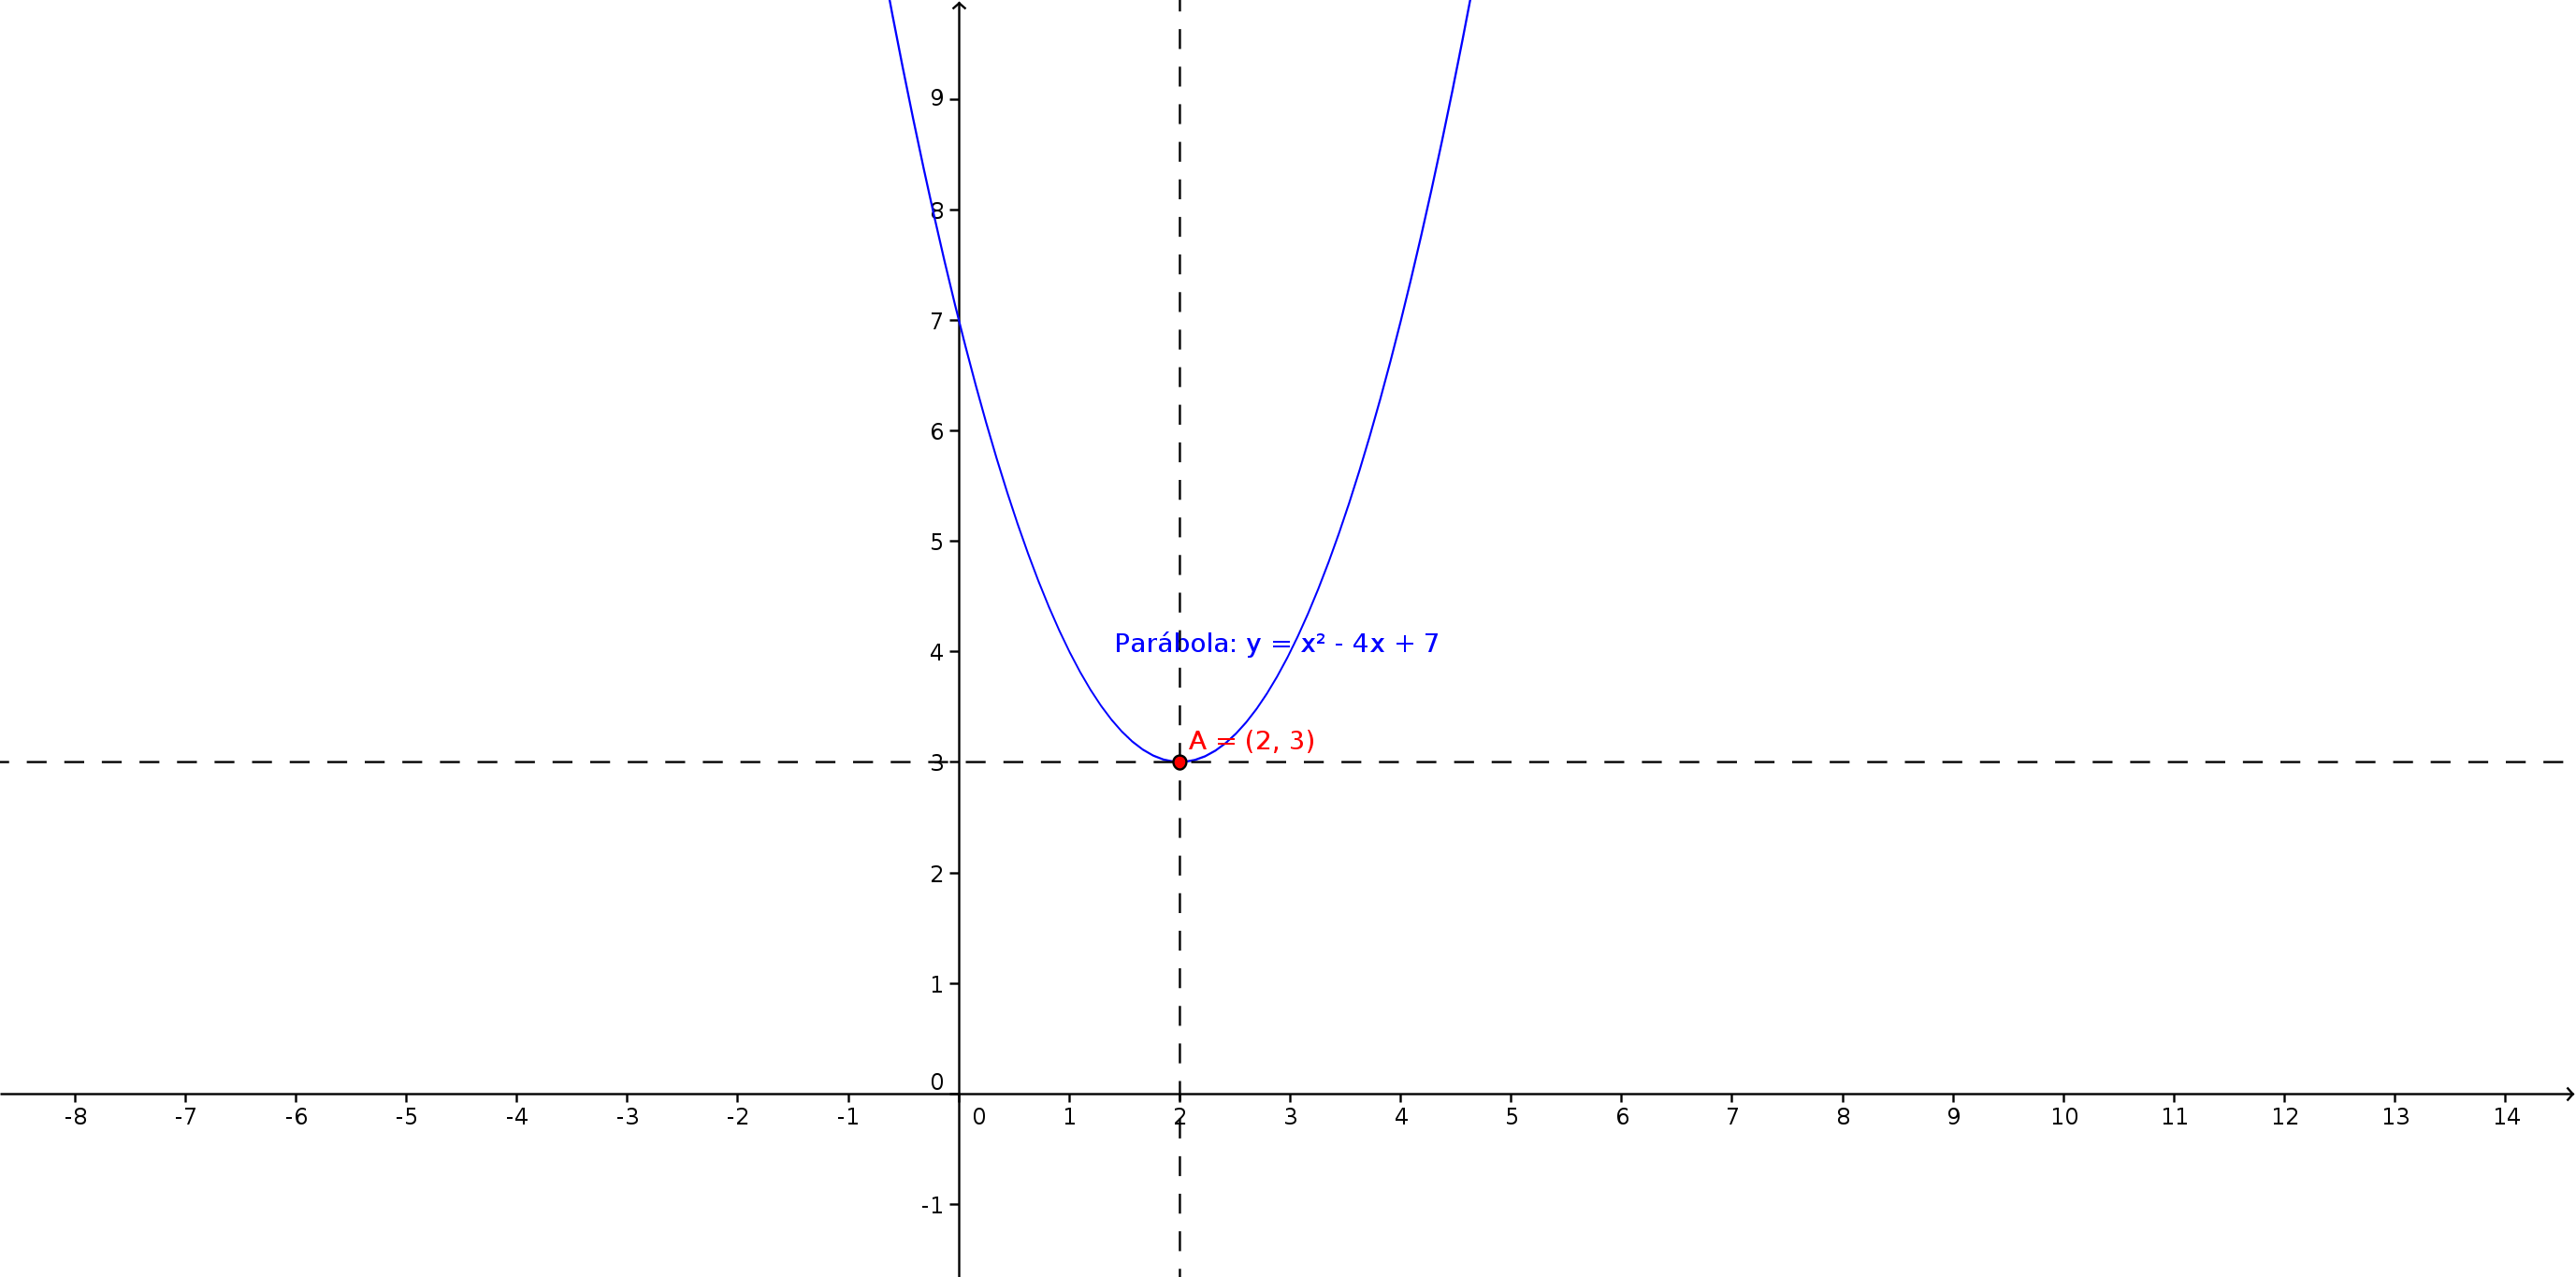
\includegraphics[height=5cm,keepaspectratio=true]{./precalculo/IM020401.png}
		% IM020401.png: 0x0 pixel, 300dpi, 0.00x0.00 cm, bb=
		\caption{$y=x^2-4x+7$}
		\label{fig:020401}
	\end{figure}
	


\subsection{Complemento de cuadrados}


	Cualquier funci\'on cuadrática se puede reescribir en la forma
	$$
	f(x)=a(x-h)^2+k,
	$$
	por el m\'etodo de \emph{complementos de cuadrado.}



	El punto $(h,k)$ se llama \emph{v\'ertice,} y corresponde al \emph{extremo} de la parábola
	$$
	y=a(x-h)^2+k.
	$$



	La f\'ormula para encontrar el v\'ertice de la parábola 
	$y=f(x)=ax^2+bx+c$ es
	$$\begin{cases}
		h=-\dfrac{b}{2a}\\
		k=f(h).
	\end{cases}
	$$ 



	Para completar el cuadrado, podemos usar el \emph{m\'etodo de divisi\'on sint\'etica:}
	\begin{center}
		\begin{tabular}{l|lll}
			$h$ & $a$ & $b$ & $c$\\
			& $\downarrow$ & $+ah$ & $\dots$\\\hline
			& $a$ & $\dots$ & $k$
		\end{tabular}
	\end{center}



	\begin{problema}
		Complete el cuadrado de
		$$y=x^2-4x+7.$$
	\end{problema}
	



	\begin{problema}
		Complete el cuadrádo de
		$$
		y=3x^2+30x+63.
		$$
	\end{problema}
	


\subsection{Intersecciones con los ejes}


	Las ra\'ices de un polinomio $p(x)$ son aquellos números reales $r$ tales que $p(r)=0.$



	Para encontrar las ra\'ices de una \emph{polinomio cuadrático}, necesitamos resolver la \emph{ecuaci\'on de segundo grado}
	$$
	a(x-h)^{2}+k=0.
	$$



	Si $r$ es una ra\'iz de $p(x)=a(x-h)^{2}+k,$ entonces la parábola $y=a(x-h)^{2}+k$ cruza al eje $x$ en el punto $(r,0).$




	\begin{observacion}
		Si bien $a,k>0$ o bien $a,k<0,$ entonces $a(x-h)^{2}+k>0$ y por tanto no existen ra\'ices. Por lo tanto, la parábola $y=a(x-h)^{2}+k$ \emph{nunca} cruza el eje $x.$ 
	\end{observacion}
	



	\begin{problema}
		Determine si existen ra\'ices de
		$$
		y=x^2-4x+7,
		$$ 
	\end{problema}
	



\subsection{Diferencia de cuadrados}


	Una identidad que es muy útil al momento de resolver ecuaciones es la \emph{diferencia de cuadrados}
	$$
	\left( a-b \right)\left( a+b \right)=a^{2}-b^{2}.
	$$



	Una ecuaci\'on de la forma 
	$$
	z^{2}-c^{2}=0
	$$
	se puede reescribir como
	$$
	\left( z-c \right)\left( z+c \right)=0...
	$$
	
	...en cuyo caso tenemos que $z-c=0$ o $z+c=0,$
	y por tanto las soluciones son
	$$
	z=\pm c.
	$$



	\begin{problema}
		Encuentre las ra\'ices de
		$$
		y=3x^2+30x+63.
		$$ 
	\end{problema}
	



	\begin{center}
		\includegraphics[height=5cm,keepaspectratio=true]{./precalculo/IM0301.png}
		% IM0301.png: 0x0 pixel, 300dpi, 0.00x0.00 cm, bb=
	\end{center}
	




\subsection{Ejemplos}


	\begin{problema} Resuelva las siguientes ecuaciones
		\begin{enumerate}
			\item $x^{2}-40=9$
			\item $2x^{2}-400=0$
			\item $x^{2}+36=9-2x^{2}$
		\end{enumerate}
		
	\end{problema}
	



	\begin{problema} Resuelva las siguientes ecuaciones
		\begin{enumerate}
			\item $\dfrac{x}{16}=\dfrac{4}{x}$
			\item $\dfrac{y^{2}}{3}=\dfrac{y^{2}}{6}+2$
		\end{enumerate}
		
	\end{problema}
	



	\begin{problema} Resuelva la siguiente ecuaci\'on
		$$
		\dfrac{1-2x}{3-x}=\dfrac{x-2}{3x-1}.
		$$
	\end{problema}
	



	\begin{problema} Resuelva la siguiente ecuaci\'on
		$$
		\dfrac{1}{2x-1}-\dfrac{1}{2x+1}=\dfrac{1}{4}.
		$$
	\end{problema}
	



	\begin{problema} Resuelva la siguiente ecuaci\'on
		$$
		x-\dfrac{2x}{x+1}=\dfrac{5}{x+1}-1.
		$$
	\end{problema}
	



	\begin{problema}
		\label{spi:exmp:16.2}
		Encuentre las ra\'ices de los siguientes polinomios
		\begin{enumerate}
			\item $7x^{2}-5x$
			\item $x^{2}-5x+6$
			\item $3x^{2}+2x-5$
			\item $x^{2}-4x+4$
		\end{enumerate}
		
	\end{problema}
	
	



	\begin{problema}
		\label{spi:exmp:16.3-}
		Encuentre las ra\'ices de los siguientes polinomios
		\begin{enumerate}
			\item $x^{2}-6x-2$
			\item $3x^2-5x+1$
			\item $4x^{2}-6x+3$   
		\end{enumerate}
		
	\end{problema}


\subsection{Factorizaci\'on}


	Si un polinomio $p(x)=ax^{2}+bx+c$ tiene ra\'ices $r_{1},r_{2}$ diferentes, entonces podemos factorizar de la siguiente manera
	$$
	p(x)=a(x-r_{1})\left( x-r_{2} \right).
	$$



	Si un polinomio $p(x)=ax^{2}+bx+c$ tiene una única ra\'z $r_{1}$, entonces podemos factorizar de la siguiente manera
	$$
	p(x)=a\left( x-r_{1} \right)^{2}.
	$$




	\begin{problema}
		\label{spi:exmp:16.2b}
		Factorice los siguientes polinomios
		\begin{enumerate}
			\item $7x^{2}-5x$
			\item $x^{2}-5x+6$
			\item $3x^{2}+2x-5$
			\item $x^{2}-4x+4$
		\end{enumerate}
		
	\end{problema}
	
	



	\begin{problema}
		\label{spi:exmp:16.3-b}
		Factorice los siguientes polinomios
		\begin{enumerate}
			\item $x^{2}-6x-2$
			\item $3x^2-5x+1$
			\item $4x^{2}-6x+3$   
		\end{enumerate}
		
	\end{problema}



\subsection{Aplicaciones}


	\begin{problema}
		\label{bron:exmp:16.21}
		Encuentre dos números positivos sabiendo que uno de ellos es igual al triple del otro más 5 y que el producto de ambos es igual a 68.
	\end{problema}
	



	\begin{problema}
		\label{bron:exmp:16.22}
		Encuentre un número sabiendo que la suma del triple del mismo con el doble de su rec\'iproco es igual a 5. 
	\end{problema}
	



	\begin{problema}
		\label{bron:exmp:16.23}
		Encuentre las dimensiones de un rectángulo cuto per\'imetro es de 50 pies y área es de 150 pies cuadrados. 
	\end{problema}



	\begin{problema}
		\label{bron:exmp:16.24}
		La hipotenusa de un triángulo es igual a 34 pulgadas. Encuentre las longitudes de los catetos sabiendo que uno de ellos es 14 pulgadas mayor que el otro.
	\end{problema}



	\begin{problema}
		\label{bron:exmp:16.25}
		Las dimensiones exteriores de un marco de fotograf\'ia son 12 por 15 pulgadas. Sabiendo que el ancho permanece constante, encuentre su valor a) cuando la superficie de la fotograf\'ia es de 88 pulgadas y b) cuando dicha superficie vale 100 pulgadas cuadradas. 
	\end{problema}



	\begin{problema}
		\label{bron:exmp:16.26}
		Un piloto realiza un vuelo de 600 millas. Sabiendo que si aumenta la velocidad en 40 millas/hora podr\'ia recorrer dicha distancia empleando 30 minutos menos, encuentre la velocidad promedio.  
	\end{problema}



	\begin{problema}
		\label{bron:exmp:16.27}
		Un comerciante compra determinado número de camisas por \$180 y las vende todas menos 6 con una ganancia de \$2 en cada camisa. Sabiendo que con el dinero recaudado en la venta podr\'ia haber comprado 30 camisas más que antes, calcule el precio de cada camisa.  
	\end{problema}



	\begin{problema}
		\label{bron:exmp:16.28}
		Dos operarios A y B juntos, realizan una tarea en 10 d\'ias. Trabajando por separado, A tardar\'ia 5 d\'ias más que B. Encuentre  el número de d\'ias que tardar\'ian en hacer la tarea trabajando cada no por s\'i s\'olo. 
	\end{problema}



\chapter{Trigonometría}


\section{La geometría de los triángulos: congruencia, similitud y el teorema de Pitágoras}

\subsection{Triángulos congruentes}

{}
	Los triángulos que tienen el mismo tamaño y la misma forma se llaman \emph{triángulos congruentes}.

{}
	\begin{center}
		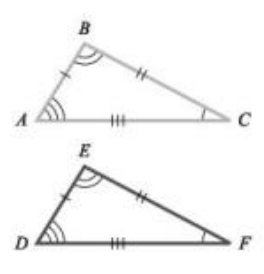
\includegraphics[height=8cm,keepaspectratio=true]{./trig/algsup3-01.png}
		% algsup3-01.png: 0x0 pixel, 300dpi, 0.00x0.00 cm, bb=
	\end{center}
	

{}
	Si dos triángulos $\triangle ABC, \triangle DEF$ son congruentes, escribiremos \begin{align*}
		\triangle ABC \cong \triangle DEF.
	\end{align*}

{}
	\begin{prop}[Criterios de congruencia]
		\begin{itemize}
			\item \emph{LAL}: Dos lados y su ángulo incluido iguales.
			\item \emph{ALA}: Dos ángulos y su lado incluido iguales. 
			\item \emph{LLL}: Tres lados iguales. 
		\end{itemize}
		
	\end{prop}
	


\subsection{Triángulos semejantes}
[t]{}
	\begin{wrapfigure}[15]{l}{5cm}
		%%%%%%%%%%%%%%%%%%%%%%%%%%%%%%%%%%%%%%%%%%%%%%%%%%%%%%%%%%%%%%%%%%%%%%%%%%%%%%%%%%%%%%%
		%%% You will need to add \usepackage{wrapfig} to your preamble to use textwrapping %%%
		%%%%%%%%%%%%%%%%%%%%%%%%%%%%%%%%%%%%%%%%%%%%%%%%%%%%%%%%%%%%%%%%%%%%%%%%%%%%%%%%%%%%%%%
		\centering
		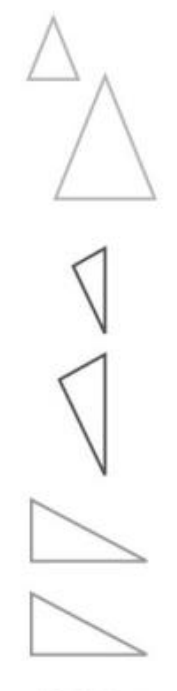
\includegraphics[width=2cm,keepaspectratio=true]{./trig/algsup3-02.png}
		% algsup3-02.png: 0x0 pixel, 300dpi, 0.00x0.00 cm, bb=
		\label{fig:3-02}
	\end{wrapfigure}
	
	Diremos que dos triángulos $\triangle ABC$ y $\triangle DEF$ son \emph{similares} si 
	existe un correspondencia $A\leftrightarrow D, B\leftrightarrow E, C \leftrightarrow F$
	tal que $\frac{|AB|}{|DE|}=\frac{|BC|}{|EF|}=\frac{|CA|}{|FD|}=: \alpha.$
	
	
	A tal \emph{constante de proporcionalidad} $\alpha$ se conoce como \emph{escala}.

{}
	\begin{prop}[Criterio \emph{AA}]
		Si las medidas de dos ángulos de un triángulo son iguales a las de dos ángulos correspondientes de un segundo triángulo, entonces los dos triángulos son semejantes.
	\end{prop}
	

[t]{}
	\begin{problema}
		\label{exmp:9405}
		\begin{wrapfigure}[15]{L}{6cm}
			%%%%%%%%%%%%%%%%%%%%%%%%%%%%%%%%%%%%%%%%%%%%%%%%%%%%%%%%%%%%%%%%%%%%%%%%%%%%%%%%%%%%%%%
			%%% You will need to add \usepackage{wrapfig} to your preamble to use textwrapping %%%
			%%%%%%%%%%%%%%%%%%%%%%%%%%%%%%%%%%%%%%%%%%%%%%%%%%%%%%%%%%%%%%%%%%%%%%%%%%%%%%%%%%%%%%%
			\centering
			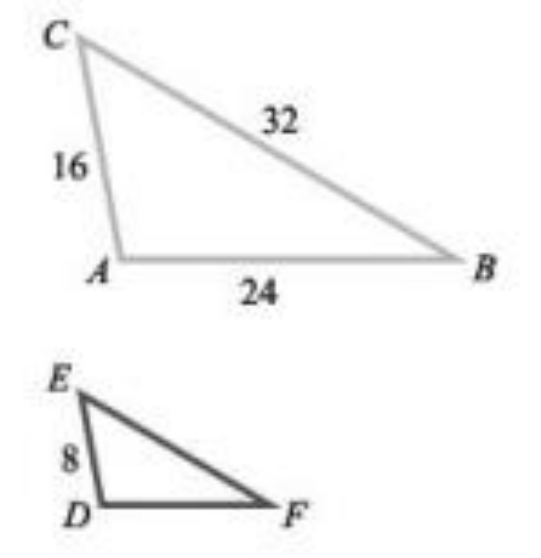
\includegraphics[width=5cm,keepaspectratio=true]{./trig/trig9446.png}
			% trig9446.png: 0x0 pixel, 300dpi, 0.00x0.00 cm, bb=
			\label{fig:9446}
		\end{wrapfigure}
		Suponga que en la figura, ambos triángulos son semejantes. Encuentre las longitudes desconocidas de los lados de $\triangle EDF.$
	\end{problema}
	

[t]{}
	\begin{problema}
		\label{exmp:9406}
		\begin{wrapfigure}[15]{L}{6cm}
			%%%%%%%%%%%%%%%%%%%%%%%%%%%%%%%%%%%%%%%%%%%%%%%%%%%%%%%%%%%%%%%%%%%%%%%%%%%%%%%%%%%%%%%
			%%% You will need to add \usepackage{wrapfig} to your preamble to use textwrapping %%%
			%%%%%%%%%%%%%%%%%%%%%%%%%%%%%%%%%%%%%%%%%%%%%%%%%%%%%%%%%%%%%%%%%%%%%%%%%%%%%%%%%%%%%%%
			\centering
			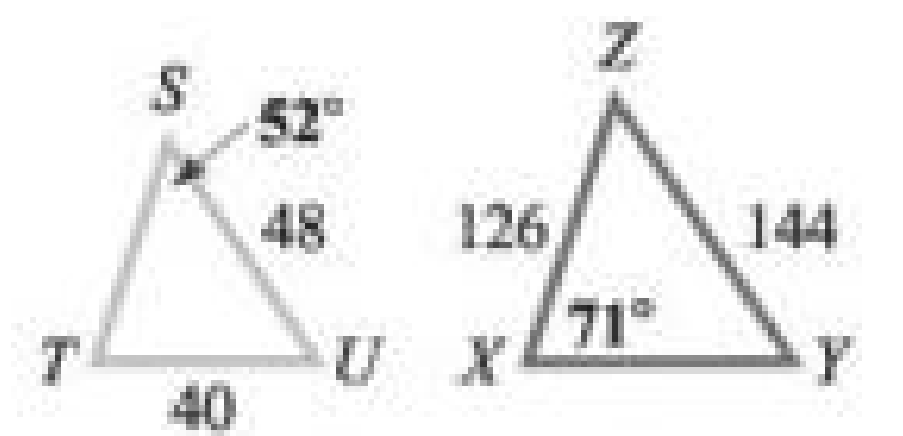
\includegraphics[width=5cm,keepaspectratio=true]{./trig/trig9447.png}
			% trig9446.png: 0x0 pixel, 300dpi, 0.00x0.00 cm, bb=
			\label{fig:9447}
		\end{wrapfigure}
		Encuentre las medidas de las partes desconocidas de los triángulos semejantes $\triangle STU$ y $\triangle ZXY.$ 
	\end{problema}
	

[t]{}
	\begin{problema}
		\label{exmp:9407}
		\begin{wrapfigure}[15]{L}{6cm}
			%%%%%%%%%%%%%%%%%%%%%%%%%%%%%%%%%%%%%%%%%%%%%%%%%%%%%%%%%%%%%%%%%%%%%%%%%%%%%%%%%%%%%%%
			%%% You will need to add \usepackage{wrapfig} to your preamble to use textwrapping %%%
			%%%%%%%%%%%%%%%%%%%%%%%%%%%%%%%%%%%%%%%%%%%%%%%%%%%%%%%%%%%%%%%%%%%%%%%%%%%%%%%%%%%%%%%
			\centering
			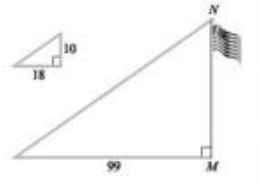
\includegraphics[width=5cm,keepaspectratio=true]{./trig/trig9448.png}
			% trig9446.png: 0x0 pixel, 300dpi, 0.00x0.00 cm, bb=
			\label{fig:9448}
		\end{wrapfigure}
		La jefa de oficina de correos de una ciudad quiere medir la altura del asta de la bandera de la oficina. Observa que en el instante en el que la sombra de la estación mide $18fts$, la sombra del asta mide $99fts$. El edificio tiene $10fts$ de altura. ¿Cuál es la altura del asta?
	\end{problema}
	

\subsection{El teorema de Pitágoras}
{}
	\begin{thm}[Pitágoras]
		\begin{wrapfigure}[10]{L}{6cm}
			%%%%%%%%%%%%%%%%%%%%%%%%%%%%%%%%%%%%%%%%%%%%%%%%%%%%%%%%%%%%%%%%%%%%%%%%%%%%%%%%%%%%%%%
			%%% You will need to add \usepackage{wrapfig} to your preamble to use textwrapping %%%
			%%%%%%%%%%%%%%%%%%%%%%%%%%%%%%%%%%%%%%%%%%%%%%%%%%%%%%%%%%%%%%%%%%%%%%%%%%%%%%%%%%%%%%%
			\centering
			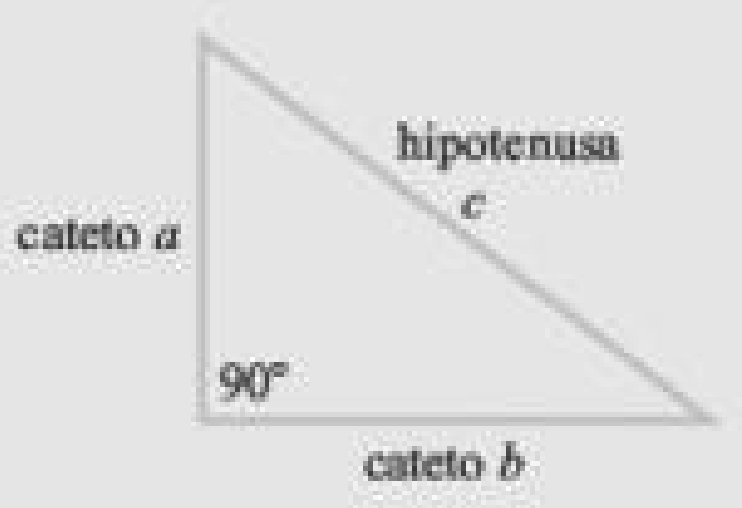
\includegraphics[width=5cm,keepaspectratio=true]{./trig/trig94thm.png}
			% trig94thm.png: 0x0 pixel, 300dpi, 0.00x0.00 cm, bb=
			\label{fig:94thm}
		\end{wrapfigure}
		\begin{align*}
			a^{2}+b^{2}=c^{2}
		\end{align*}
	\end{thm}
	

{}
	Los números naturales $\set{3,4,5}$ forman una \emph{terna pitagórica}, ya que satisfacen las ecuaciones del teorema de Pitágoras. 

[t]{}
	\begin{problema}
		\label{exmp:9408}
		\begin{wrapfigure}[5]{l}{5cm}
			%%%%%%%%%%%%%%%%%%%%%%%%%%%%%%%%%%%%%%%%%%%%%%%%%%%%%%%%%%%%%%%%%%%%%%%%%%%%%%%%%%%%%%%
			%%% You will need to add \usepackage{wrapfig} to your preamble to use textwrapping %%%
			%%%%%%%%%%%%%%%%%%%%%%%%%%%%%%%%%%%%%%%%%%%%%%%%%%%%%%%%%%%%%%%%%%%%%%%%%%%%%%%%%%%%%%%
			\centering
			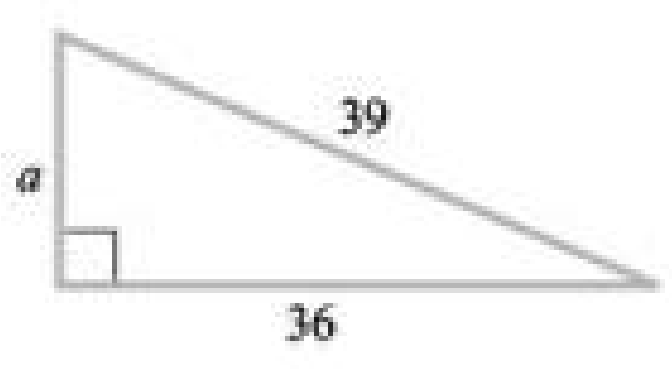
\includegraphics[width=5cm,keepaspectratio=true]{./trig/trig9450.png}
			% trig9450.png: 0x0 pixel, 300dpi, 0.00x0.00 cm, bb=
			\label{fig:9450}
		\end{wrapfigure}
		
		Determine la longitud $a$ del triángulo rectángulo que se muestra.
	\end{problema}
	

[t]{}
	\begin{problema}
		\label{exmp:9409}
		\begin{wrapfigure}[5]{l}{5cm}
			%%%%%%%%%%%%%%%%%%%%%%%%%%%%%%%%%%%%%%%%%%%%%%%%%%%%%%%%%%%%%%%%%%%%%%%%%%%%%%%%%%%%%%%
			%%% You will need to add \usepackage{wrapfig} to your preamble to use textwrapping %%%
			%%%%%%%%%%%%%%%%%%%%%%%%%%%%%%%%%%%%%%%%%%%%%%%%%%%%%%%%%%%%%%%%%%%%%%%%%%%%%%%%%%%%%%%
			\centering
			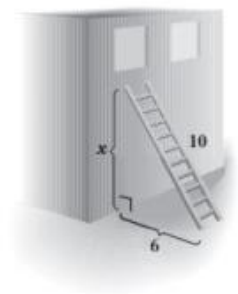
\includegraphics[width=5cm,keepaspectratio=true]{./trig/trig9451.png}
			% trig9450.png: 0x0 pixel, 300dpi, 0.00x0.00 cm, bb=
			\label{fig:9451}
		\end{wrapfigure}
		Una escalera de 10 metros de longitud tiene su base a 6 metros de la pared. ¿Qué altura alcanza la escalera?
	\end{problema}
	


\section{Los ángulos y sus medidas}
\subsection{Terminología básica}
{}
	\begin{figure}[h]
		\centering
		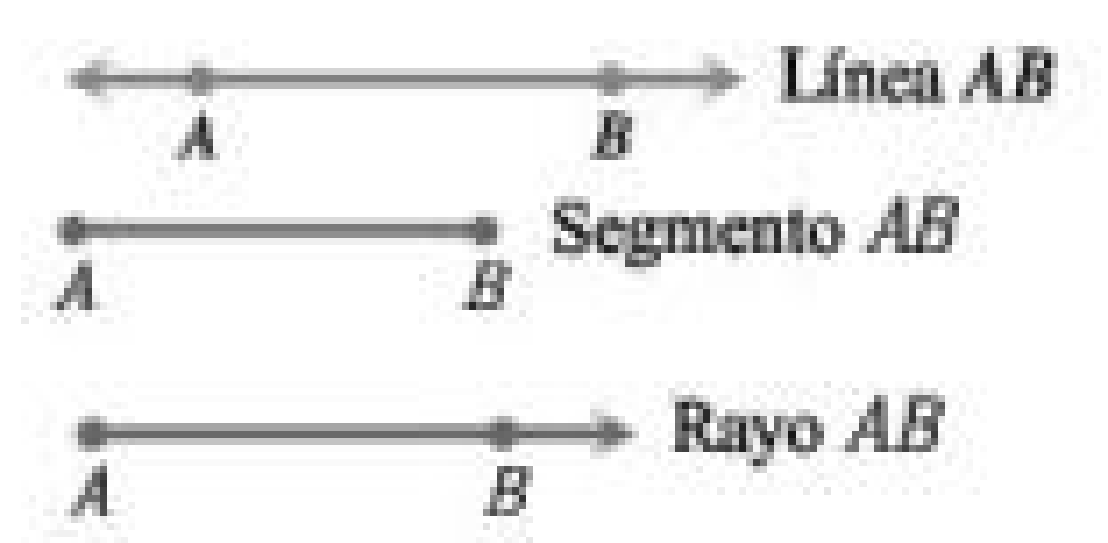
\includegraphics[width=10cm,keepaspectratio=true]{./trig/trig_101-1.png}
		% trig_10.1-1.png: 0x0 pixel, 300dpi, 0.00x0.00 cm, bb=
		\label{fig:101-1}
	\end{figure}
	

{}
	\begin{figure}[h]
		\centering
		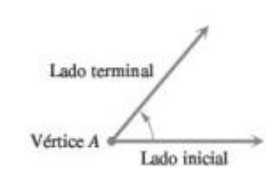
\includegraphics[width=10cm,keepaspectratio=true]{./trig/trig_101-2.png}
		% trig_10.1-1.png: 0x0 pixel, 300dpi, 0.00x0.00 cm, bb=
		\label{fig:101-2}
	\end{figure}
	

{}
	\begin{figure}[h]
		\centering
		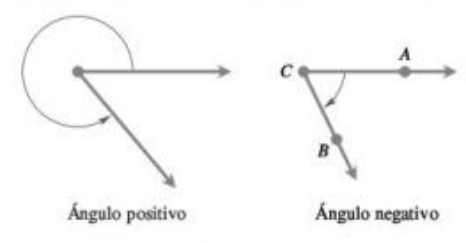
\includegraphics[width=10cm,keepaspectratio=true]{./trig/trig_101-3.png}
		% trig_10.1-1.png: 0x0 pixel, 300dpi, 0.00x0.00 cm, bb=
		\label{fig:101-3}
	\end{figure}
	

{}
	\begin{figure}[h]
		\centering
		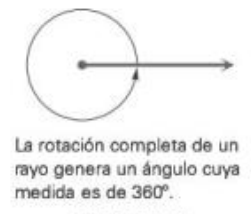
\includegraphics[width=10cm,keepaspectratio=true]{./trig/trig_101-4.png}
		% trig_10.1-1.png: 0x0 pixel, 300dpi, 0.00x0.00 cm, bb=
		\label{fig:101-4}
	\end{figure}
	

{}
	\begin{figure}[h]
		\centering
		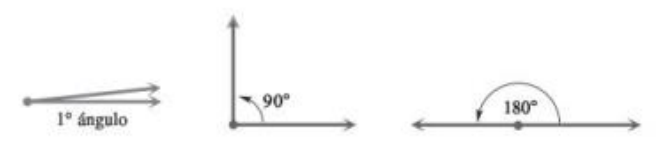
\includegraphics[width=10cm,keepaspectratio=true]{./trig/trig_101-5.png}
		% trig_10.1-1.png: 0x0 pixel, 300dpi, 0.00x0.00 cm, bb=
		\label{fig:101-5}
	\end{figure}
	

{}
	\begin{figure}[h]
		\centering
		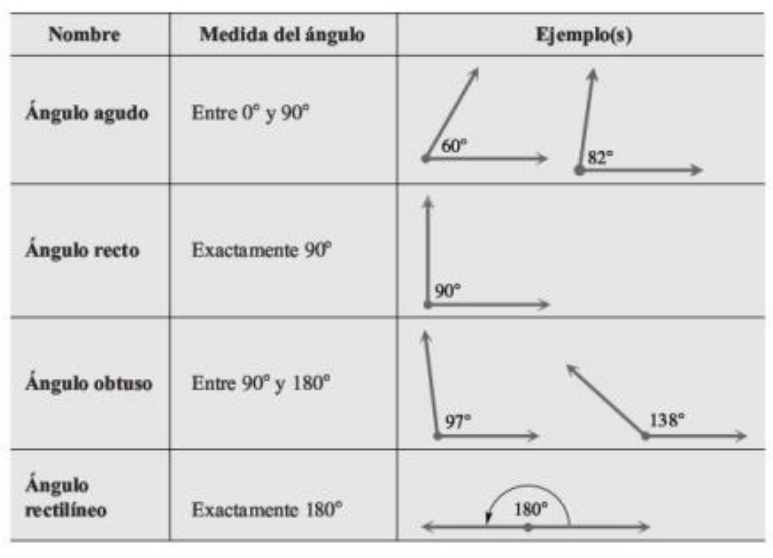
\includegraphics[width=8cm,keepaspectratio=true]{./trig/trig_101-tab1.png}
		% trig_101-tab1.png: 0x0 pixel, 300dpi, 0.00x0.00 cm, bb=
		\label{fig:101-tab1}
	\end{figure}
	

{}
	Si la suma de las medidas de  dos ángulos es $90^{o},$ los ángulos se llaman \emph{complementarios}. En tanto que dos ángulos cuyas medidas sumen $180^{o}$ son \emph{suplementarios}.

{}
	\begin{problema}
		\label{exmp:1011}
		Diga cuál es el complemento y el suplemento de $50^{o}$.
	\end{problema}
	

\subsection{Radianes}
{}
	Un \emph{ángulo central} es un ángulo positivo cuyo vértice esta en el centro de un círculo. 

{}
	\begin{figure}[h]
		\centering
		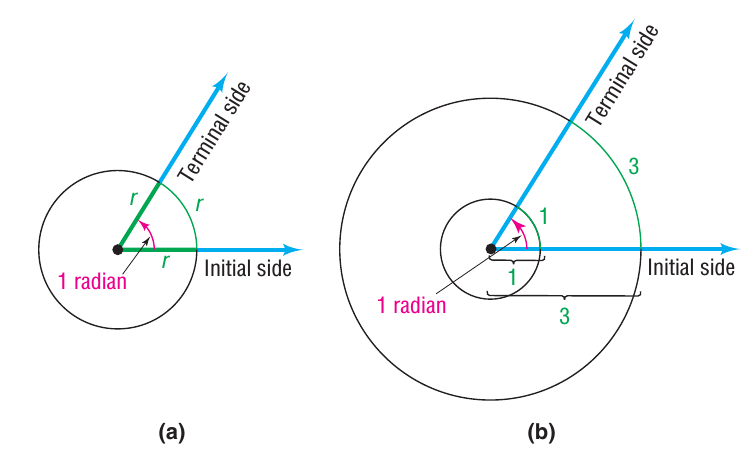
\includegraphics[height=5cm,keepaspectratio=true]{./trig/sull0610.png}
		% sull0610.png: 0x0 pixel, 300dpi, 0.00x0.00 cm, bb=
		\label{fig:sull6110}
	\end{figure}
	

{}
	\begin{thm}[Longitud de arco]
		Para un círculo de radio $r$, un ángulo central  de $\theta$ radianes subtiende un arco cuya longitud es 
		\begin{align}
			\label{sull6104}
			s = r\theta
		\end{align}
	\end{thm}
	

{}
	\begin{problema}
		\label{exmp:sull6103}
		Encuentre la longitud de arco de un círculo de radio $2$ subtendido por un ángulo central de $0.25$ radianes. 
	\end{problema}

{}
	\begin{problema}
		\label{exe:sull6171}
		Encuentre la longitud de arco de un círculo de radio $10$ subtendido por un ángulo central de $\frac{1}{2}$ radianes. 
	\end{problema}
	

\subsection{Conversión entre grados y radianes}
{}
	\begin{figure}[h]
		\centering
		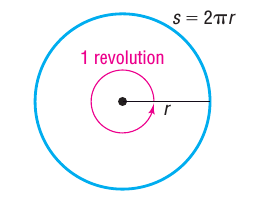
\includegraphics[height=5cm,keepaspectratio=true]{./trig/sull6112.png}
		% sull6112.png: 0x0 pixel, 300dpi, 0.00x0.00 cm, bb=
		\label{fig:sull6112}
		\caption{1 revolución = $2\pi$ radianes}
	\end{figure}
	

{}
	Como una revolución equivale a $360^{o},$ entonces $1 \texttt{rad}=360^{0}.$ De manera simplificada:
	\begin{align*}
		180^{o}= \pi\texttt{rad}
	\end{align*}

{}
	\begin{problema}
		Convierta cada uno de los ángulos a radianes:
		\begin{itemize}
			\item $60^{o}=$ 
			\item $150^{o}=$ 
			\item $-45^{o}=$ 
			\item $90^{o}=$ 
			\item $107^{o}$ 
		\end{itemize}
		
	\end{problema}
	

{}
	\begin{problema}
		\begin{itemize}
			\item Convierta $35^{o}$ a radianes, expresándolo como un múltiplo de $\pi$.
			\item Convierta $-40^{o}$ a radianes, expresándolo en decimales. 
		\end{itemize}
		
	\end{problema}
	

{}
	\begin{figure}[h]
		\centering
		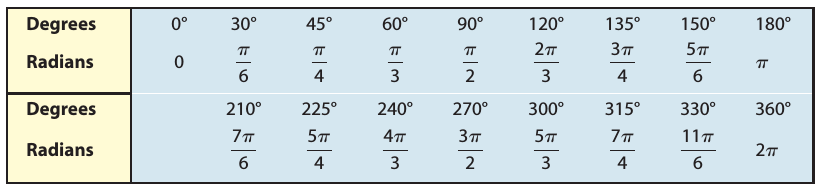
\includegraphics[width=10cm,keepaspectratio=true]{./trig/sull61t1.png}
		% sull61t1.png: 0x0 pixel, 300dpi, 0.00x0.00 cm, bb=
		\label{fig:61t1}
	\end{figure}
	

{}
	\begin{problema}
		La latitud de una locación $L$ es la medida del ángulo formado por un rayo dibujado desde el centro de la tierra al ecuador y un rayo dibujado del centro de la tierra a $L$. 
		
		Glasgow, Montana está al norte de Albuquerque, Nuevo México. Encuentre la distancia entre Glasgow, $48^{o}, 9'$, latitud Norte y Albuquerque, $35^{o}, 5'$. Suponga que el radio de la tierra es $3960$ millas.
	\end{problema}
	

{}
	\begin{figure}[h]
		\centering
		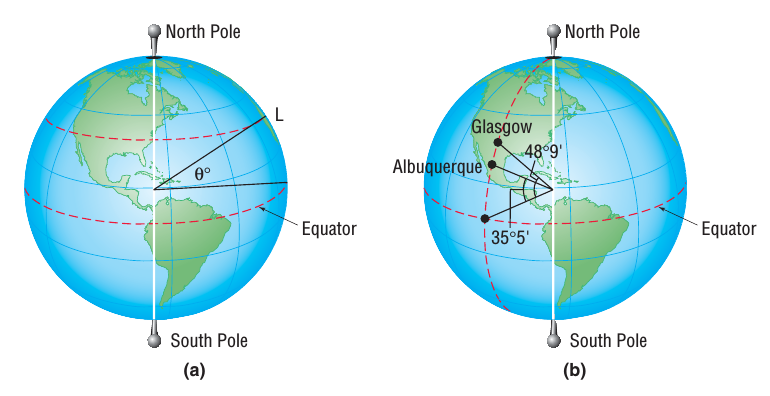
\includegraphics[width=10cm,keepaspectratio=true]{./trig/sull113.png}
		% sull113.png: 0x0 pixel, 300dpi, 0.00x0.00 cm, bb=
		\label{fig:sull6113}
	\end{figure}
	

{}
	\begin{problema}
		Memphis, Tennessee, está al norte de Nueva Orleans, Lousiana. Encuentre la distancia entre Memphis, $35^{o}, 9'$ latitud norte, y Nueva Orleans, $29^{o}, 57'$ latitud norte. Suponga que el radio de la tierra es $3960$ millas. 
	\end{problema}
	

\subsection{Área de un sector de un círculo} 
{}
	\begin{figure}[h]
		\centering
		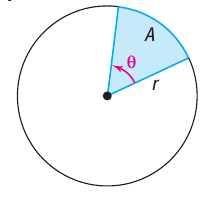
\includegraphics[height=5cm,keepaspectratio=true]{./trig/sull614.png}
		% sull614.png: 0x0 pixel, 300dpi, 0.00x0.00 cm, bb=
		\label{fig:sull6114}
	\end{figure}

{}
	\begin{figure}[h]
		\centering
		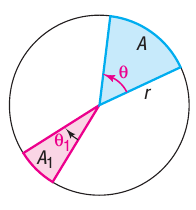
\includegraphics[height=5cm,keepaspectratio=true]{./trig/sull6115.png}
		% sull614.png: 0x0 pixel, 300dpi, 0.00x0.00 cm, bb=
		\label{fig:sull6115}
	\end{figure}

{}
	\begin{thm}[Área de un sector]
		El área $A$ de un sector de un círculo de radio $r$ formado por un ángulo central de $\theta$ radianes es 
		\begin{align}
			\label{sull6108}
			A=\frac{1}{2}r^{2}\theta.
		\end{align}
	\end{thm}
	

{}
	\begin{problema}
		\label{exmp:sull6107}
		Encuentre el área del sector de un círculo de radio $2fts$ formado por un ángulo de $30^{o}$. Redondee la respuesta dos decimales.  
	\end{problema}
	

{}
	\begin{problema}
		Encuentre el área del sector de un círculo de radio $10m$ formado por un ángulo de $\frac{1}{2}rad$. Redondee la respuesta dos decimales.  
	\end{problema}
	

\subsection{Movimiento circular}
{}
	\begin{figure}[h]
		\centering
		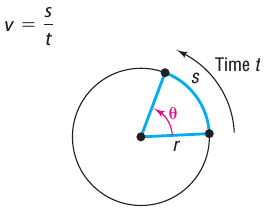
\includegraphics[height=5cm,keepaspectratio=true]{./trig/sull6116.png}
		% sull6116.png: 0x0 pixel, 300dpi, 0.00x0.00 cm, bb=
		\label{fig:sull6116}
	\end{figure}
	

{}
	Supongamos que un objeto se mueve alrededor de un círculo de radio $r$ a una rapidez constante. Si $s$ es la distancia recorrida en un tiempo $t$ alrededor del círculo, entonces la \emph{rapidez lineal} $v$ de este objeto se define como
	\begin{align}
		\label{sull6109}
		v=\dfrac{s}{t}
	\end{align}

{}
	La \emph{rapidez angular} $\om$ de este objeto es el ángulo $\theta$ (medido en radianes) barrido, dividido por el lapso $t$, es decir, 
	\begin{align}
		\label{sull6110}
		\om=\dfrac{\theta}{t}.
	\end{align}
	
	De manera que 
	\begin{align}
		\label{sull6111}
		v = r\om.
	\end{align}

{}
	\begin{wrapfigure}{l}{6cm}
		%%%%%%%%%%%%%%%%%%%%%%%%%%%%%%%%%%%%%%%%%%%%%%%%%%%%%%%%%%%%%%%%%%%%%%%%%%%%%%%%%%%%%%%
		%%% You will need to add \usepackage{wrapfig} to your preamble to use textwrapping %%%
		%%%%%%%%%%%%%%%%%%%%%%%%%%%%%%%%%%%%%%%%%%%%%%%%%%%%%%%%%%%%%%%%%%%%%%%%%%%%%%%%%%%%%%%
		\centering
		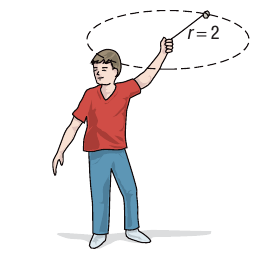
\includegraphics[width=5cm,keepaspectratio=true]{./trig/sull6117.png}
		% sull6117.png: 0x0 pixel, 300dpi, 0.00x0.00 cm, bb=
		\label{fig:6117}
	\end{wrapfigure}
	\begin{problema}
		\label{exmp:6108}
		Una persona está haciendo una roca atada al extremo de un cuerda de $2fts$ a un ritmo de $180rpm$. Encuentre la rapidez lineal de la roca en el instante en que es liberada.
	\end{problema}
	

{}
	\begin{problema}
		\label{exe:sull6197}
		Un objeto está viajando alrededor de un círculo de radio $5cm$. Si en $20s$ un ángulo central de $\dfrac{1}{3}rad$ es barrido, ¿cuál es su rapidez angular? ¿Cuál es su rapidez lineal?
	\end{problema}
	


	

\section{Funciones trigonométricas: El enfoque del círculo unitario}
\subsection{El círculo unitario}
{}
	\begin{figure}[h]
		\centering
		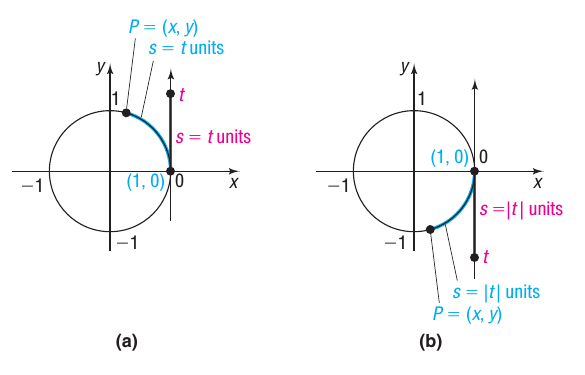
\includegraphics[width=10cm,keepaspectratio=true]{./trig/sull0618.png}
		% sull0618.png: 0x0 pixel, 300dpi, 0.00x0.00 cm, bb=
		\label{fig:0618}
	\end{figure}
	

{}
	\begin{defn}[Funciones trigonométricas]
		Sea $t$ un número real y $P=(x,y)$ el punto en el círculo unitario que corresponde a $t$.
		\begin{multicols}{2}
			\begin{itemize}
				\item $\sin(t)=y$
				\item $\cos(t)=x$
				\item $\tan(t)=\frac{y}{x}$
				\item $\csc(t)=\frac{1}{y}$
				\item $\sec(t)=\frac{1}{x}$
				\item $\cot(t)=\frac{x}{y}$
			\end{itemize}
		\end{multicols}
	\end{defn}

{}
	\begin{problema}
		\label{exmp:sull0601}
		Sea $t$ un número real y $P=\left(-\dfrac{1}{2}, \dfrac{\sqrt{3}}{2}  \right)$
		un punto en el círculo unitario que corresponde a $t$.  Encuentre los valores de las seis funciones trigonométricas.
	\end{problema}
	

{}
	\begin{figure}[h]
		\centering
		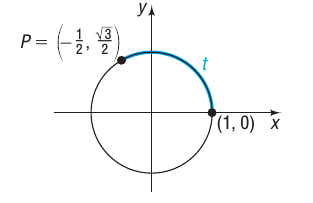
\includegraphics[width=10cm,keepaspectratio=true]{./trig/sull0619.png}
		% sull0618.png: 0x0 pixel, 300dpi, 0.00x0.00 cm, bb=
		\label{fig:0619}
	\end{figure}

{}
	\begin{problema}
		Sea $t$ un número real y $P=\left(\dfrac{\sqrt{3}}{2}, \dfrac{1}{2} \right)$
		un punto en el círculo unitario que corresponde a $t$. Encuentre los valores de las seis funciones trigonométricas.
	\end{problema}
	

\subsection{Funciones trigonométricas de ángulos}
{}
	\begin{figure}[h]
		\centering
		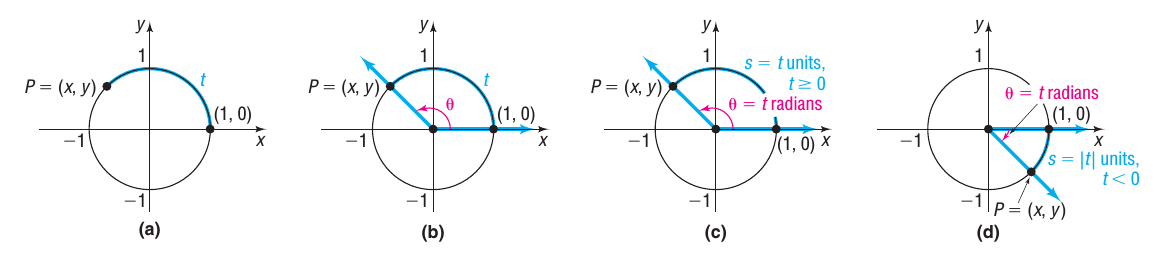
\includegraphics[width=10cm,keepaspectratio=true]{./trig/sull0620.png}
		% sull0618.png: 0x0 pixel, 300dpi, 0.00x0.00 cm, bb=
		\label{fig:0620}
	\end{figure}

{}
	Entonces, podemos definir una función trigonométrica en ángulos siempre y cuando este medido en radianes:
	\begin{align*}
		f(\theta)=f(t \texttt{ radianes})
	\end{align*} si $\theta= t \texttt{ radianes}$.

{}
	\begin{problema}
		\label{exmp:sull0602}
		Encuentre el valor exacto de las seis funciones trigonométricas en:
		\begin{itemize}
			\item $\theta=0=0^{o}$
			\item $\theta=\frac{\pi}{2}=90^{o}$ 
			\item $\theta=\pi=180^{o}$ 
			\item $\theta=\frac{3\pi}{2}=270^{o}$
		\end{itemize}
		
	\end{problema}
	

{}
	\begin{figure}[h]
		\centering
		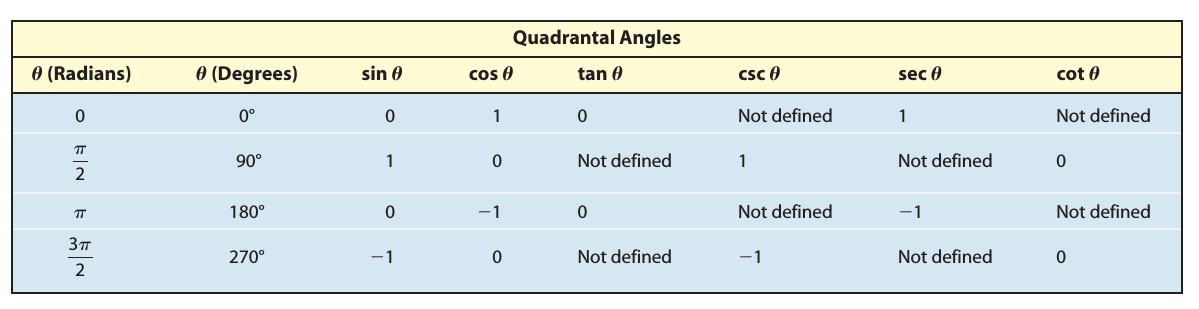
\includegraphics[width=11cm,keepaspectratio=true]{./trig/sull06t2.png}
		% sull06t2.png: 0x0 pixel, 300dpi, 0.00x0.00 cm, bb=
		\label{fig:06t2}
	\end{figure}
	

{}
	\begin{problema}
		\label{exmp:sull0603}
		Encuentre el valor exacto de:
		\begin{itemize}
			\item $\sin(3\pi)$ 
			\item $\cos(-270^{o})$
		\end{itemize}
	\end{problema}
	

{}
	\begin{problema}
		\label{exmp:sull0604}
		Encuentre el valor exacto de las seis funciones trigonométricas en $\frac{\pi}{4}=45^{o}$.
	\end{problema}
	

{Valor exacto en $\frac{\pi}{4}$}
	\begin{problema}
		\label{exmp:sull0605}
		Encuentre el valor exacto de cada expresión:
		\begin{itemize}
			\item $\sin(45^{o})\cos(180^{o})$
			\item $\tan\left( \frac{\pi}{4} \right)-\sin\left( \frac{3\pi}{2} \right)$
			\item $\left( \sec\frac{\pi}{4} \right)^{2}+\csc\frac{\pi}{2}$
		\end{itemize}
		
	\end{problema}
	

{Valor exacto en $\frac{\pi}{6}$ y $\frac{\pi}{3}$}
	\begin{figure}[h]
		\centering
		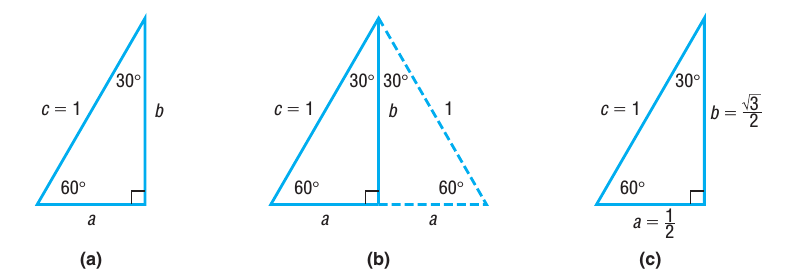
\includegraphics[width=10cm,keepaspectratio=true]{./trig/sull0624.png}
		% sull0624.png: 0x0 pixel, 300dpi, 0.00x0.00 cm, bb=
		\label{fig:0624}
	\end{figure}
	

{}
	\begin{problema}
		\label{exmp:0606}
		Encuentre el valor exacto de las seis funciones trigonométricas de $\frac{\pi}{3}=60^{o}$.
	\end{problema}
	

{}
	\begin{problema}
		\label{exmp:0607}
		Encuentre el valor exacto de las seis funciones trigonométricas de $\frac{\pi}{6}=30^{o}$.
	\end{problema}
	

{}
	\begin{figure}[h]
		\centering
		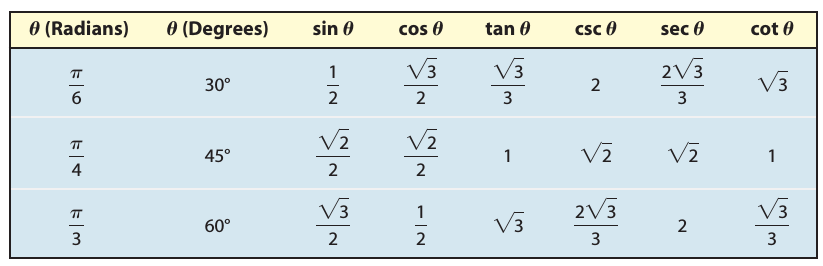
\includegraphics[width=11cm,keepaspectratio=true]{./trig/sull06t3.png}
		% sull06t3.png: 0x0 pixel, 300dpi, 0.00x0.00 cm, bb=
		\label{fig:tab3}
	\end{figure}
	

{}
	\begin{problema}
		Un recolector de lluvia se construye a partir de planchas de aluminio de 12 pulgadas de ancho. Después de marcar 4 pulgadas a partir de cada extremo, está longitud se dobla a un ángulo $\theta$. Encuentre el área transversal máxima del recolector. 
	\end{problema}


	\begin{figure}[h]
		\centering
		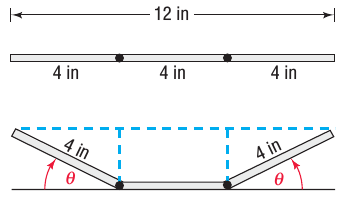
\includegraphics[width=10cm,keepaspectratio=true]{./trig/sull0627.png}
		% sull0627.png: 0x0 pixel, 300dpi, 0.00x0.00 cm, bb=
		\label{fig:0627}
	\end{figure}



\section{Funciones trigonométricas inversas}

\subsection{Funciones inversas}
{}
	Sea $f:A\to B$ una función. Diremos que $f$ es \emph{invertible} si para cada $y\in B$ \emph{siempre} corresponde un \emph{único} $x\in A$, tal que
	\begin{align*}
		f(x)=y.
	\end{align*}

{}
	Si una función $f$ es invertible, entonces existe una función $g:B\to A$ tal que $y=f(x)$ si y solo si $g(y)=x$.  En otras palabras, podemos despejar $x$.  Es usual denotar a tal función $g$ por $f^{-1}$ y llamarle \emph{inversa de $f$}.

{Propiedades del inversa}
	\begin{itemize}
		\item $f^{-1}\left( f(p) \right)$ para todo $p\in A.$ 
		\item $f\left( f^{-1}(p) \right)$ para todo $p\in B.$ 
		\item $\texttt{Dominio}(f)=\texttt{Rango}(f^{-1})$ y viceversa. 
		\item La gráfica de $f^{-1}$ es la reflexión a $45^{o}$ de la gráfica de $f$.
	\end{itemize}
	

% \subsection{Seno inverso}
% {}
% \begin{figure}[h]
%  \centering
%  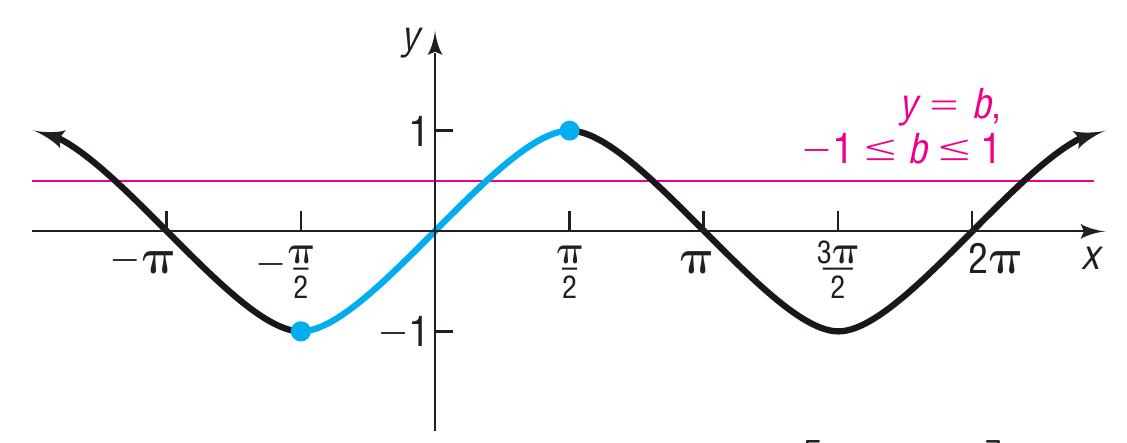
\includegraphics[width=11cm,keepaspectratio=true]{./trig/sull0701.png}
%  % sull0701.png: 0x0 pixel, 300dpi, 0.00x0.00 cm, bb=
%  \label{fig:0701}
%  \caption{$y=\sin(x), -\infty<x<\infty, -1\leq y \leq 1$}
% \end{figure}
% 
% 
% {}
% \begin{figure}[h]
%  \centering
%  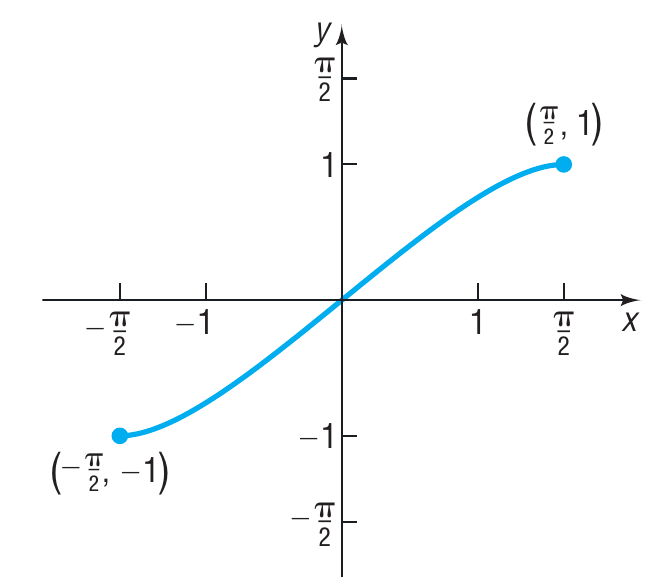
\includegraphics[height=7cm,keepaspectratio=true]{./trig/sull0702.png}
%  % sull0702.png: 0x0 pixel, 300dpi, 0.00x0.00 cm, bb=
%  \caption{$y=\sin(x), -\frac{\pi}{2}\leq x \leq \frac{\pi}{2}, -1\leq y \leq 1$}
%  \label{fig:0702}
% \end{figure}
% 
% 
% {}
% \begin{figure}[h]
%  \centering
%  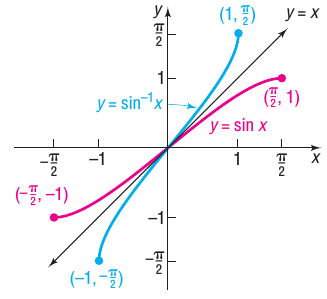
\includegraphics[height=6cm,keepaspectratio=true]{./trig/sull0703.png}
%  % sull0703.png: 0x0 pixel, 300dpi, 0.00x0.00 cm, bb=
%  \caption{$y=\sin^{-1}x, -1\leq x \leq 1, -\dfrac{\pi}{2}\leq y \leq \dfrac{\pi}{2}$}
%  \label{fig:0703}
% \end{figure}
% 
% 
% {Seno inverso}
% $$
% y = \sin^{-1} \iff
% \begin{cases}
%  x=\sin(y)\\
%  -1 \leq x \leq 1 \\
%  -\dfrac{\pi}{2} \leq y \leq \dfrac{\pi}{2}
% \end{cases}
% $$
% 
% {}
% \begin{problema}
%  Encuentre el valor exacto de
%  \begin{itemize}
%   \item $\sin^{-1}(1)$ 
%   \item $\sin^{-1}(0)$ 
%   \item $\sin^{-1}\left( -\frac{1}{2} \right)$ 
%   \item $\sin^{-1}\left( \frac{\sqrt{2}}{2} \right)$
%  \end{itemize}
% 
% \end{problema}
% 
% 
% {}
% \begin{problema}
%  Encuentre el valor exacto de 
%  \begin{itemize}
%   \item $\sin^{-1}\left( \sin\left( \frac{\pi}{8} \right) \right)$
%   \item $\sin^{-1}\left( \sin\left( \frac{5\pi}{8} \right) \right)$
%  \end{itemize}
% 
% \end{problema}
% 
% 
% {}
% \begin{problema}
%  Encuentre el valor exacto de 
%  \begin{itemize}
%   \item $\sin\left( \sin^{-1}(0.5) \right)$ 
%   \item $\sin\left( \sin^{-1}(1.8) \right)$ 
%   \item $\sin\left( \sin^{-1}\left( \frac{1}{4} \right) \right)$
%  \end{itemize}
% 
% \end{problema}
% 
% 

% \subsection{Coseno inverso}
% {}
% \begin{figure}[h]
%  \centering
%  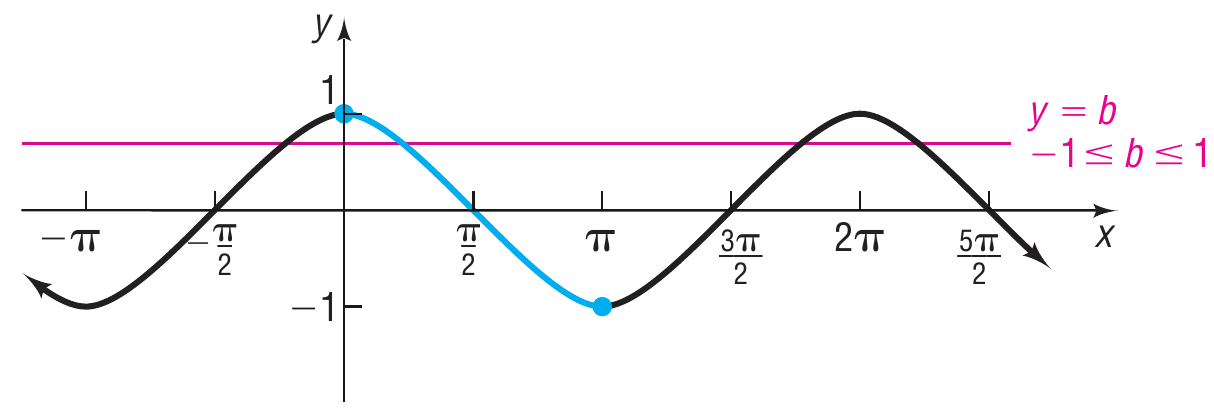
\includegraphics[width=10cm,keepaspectratio=true]{./trig/sull0707.png}
%  % sull0707.png: 0x0 pixel, 300dpi, 0.00x0.00 cm, bb=
%  \caption{$y=\cos(x),-\infty < x <\infty, -1\leq y \leq 1$}
%  \label{fig:0707}
% \end{figure}
% 
% 
% {}
% \begin{figure}[h]
%  \centering
%  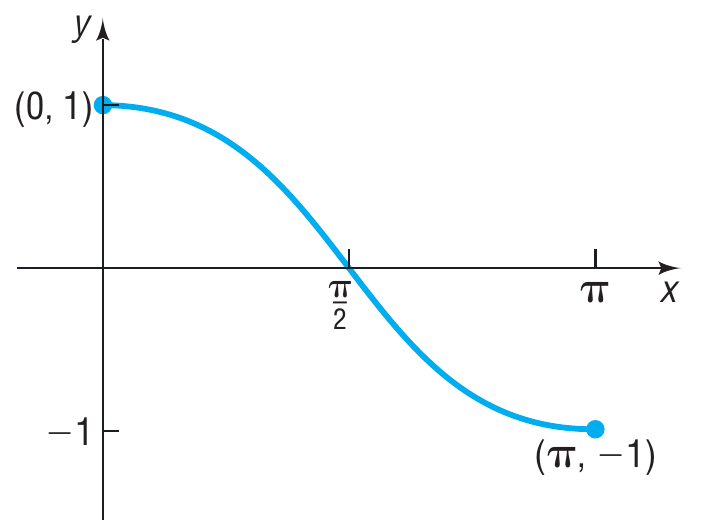
\includegraphics[width=10cm,keepaspectratio=true]{./trig/sull0708.png}
%  % sull0708.png: 0x0 pixel, 300dpi, 0.00x0.00 cm, bb=
%  \caption{$y=\cos(x),0 \leq x \leq \pi, -1\leq y \leq 1$}
%  \label{fig:0708}
% \end{figure}
% 
% 
% {}
% \begin{figure}[h]
%  \centering
%  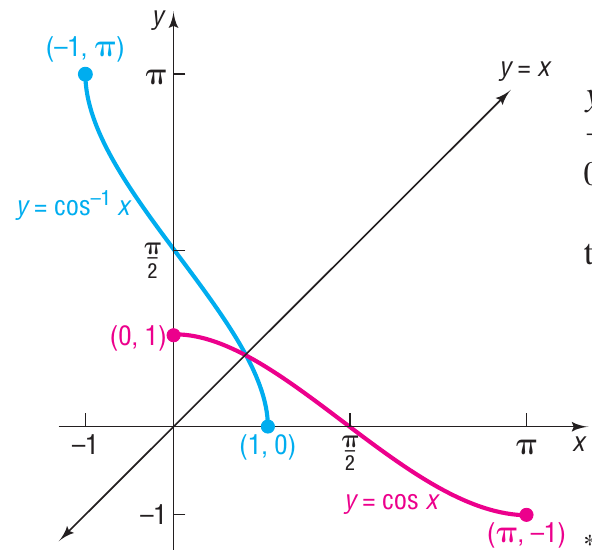
\includegraphics[width=7cm,keepaspectratio=true]{./trig/sull0709.png}
%  % sull0709.png: 0x0 pixel, 300dpi, 0.00x0.00 cm, bb=
%  \caption{$y=\cos(x), -1\leq x \leq 1, 0\leq y \leq \pi$}
%  \label{fig:0709}
% \end{figure}
% 
% 
% {Coseno inverso}
% $$y=\cos^{-1}(x)\iff
% \begin{cases}
%  x=\cos(y) \\
%  -1\leq x \leq 1 \\
%  0 \leq y \leq \pi
% \end{cases}
% $$
% 
% {}
% \begin{problema} Encuentre el valor exacto de
%  \begin{itemize}
%   \item $\cos^{-1}(0)$ 
%   \item $\cos^{-1}\left( -\frac{\sqrt{2}}{2} \right)$
%  \end{itemize}
% 
% \end{problema}
% 
% 
% {}
% \begin{problema}
%  Encuentre el valor exacto de:
%  \begin{itemize}
%   \item $\cos^{1}\left( \cos\frac{\pi}{12} \right)$
%   \item $\cos\left( \cos^{-1}(-0.4) \right)$ 
%   \item $\cos^{-1}\left( \cos\left( -\frac{2\pi}{3} \right) \right)$ 
%   \item $\cos\left( \cos^{-1}\pi \right)$
%  \end{itemize}
% 
% \end{problema}
% 
% 

\subsection{Tangente inversa}
{}
	\begin{figure}[h]
		\centering
		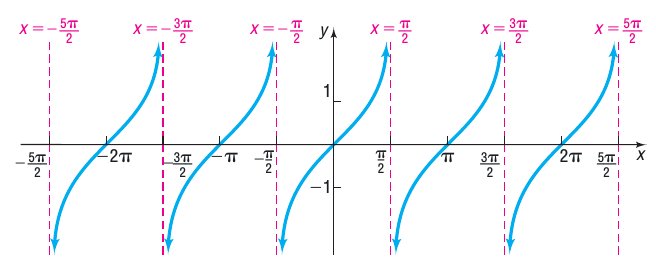
\includegraphics[width=10cm,keepaspectratio=true]{./trig/sull0712.png}
		% sull0712.png: 0x0 pixel, 300dpi, 0.00x0.00 cm, bb=
		\label{fig:0712}
		\caption{$y=\tan(x)$}
	\end{figure}
	

{}
	\begin{figure}[h]
		\centering
		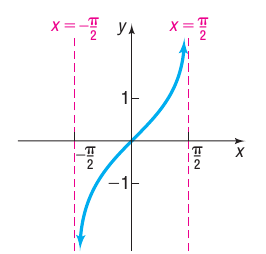
\includegraphics[height=7cm,keepaspectratio=true]{./trig/sull0713.png}
		% sull0713.png: 0x0 pixel, 300dpi, 0.00x0.00 cm, bb=
		\caption{$y=\tan(x), \; -\frac{\pi}{2}<x<\frac{\pi}{2}, \; 
			-\infty < x < \infty$}
		\label{fig:0713}
	\end{figure}
	

{}
	\begin{figure}[h]
		\centering
		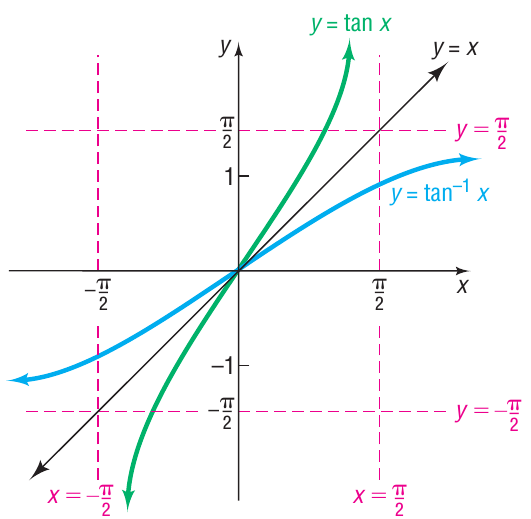
\includegraphics[height=7cm,keepaspectratio=true]{./trig/sull0714.png}
		% sull0714.png: 0x0 pixel, 300dpi, 0.00x0.00 cm, bb=
		\label{fig:0714}
	\end{figure}
	

{}
	\begin{figure}[h]
		\centering
		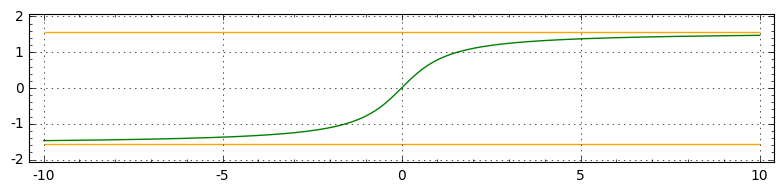
\includegraphics[width=10cm,keepaspectratio=true]{./trig/arctan.png}
		% arctan.png: 0x0 pixel, 300dpi, 0.00x0.00 cm, bb=
		\caption{$y=\tan^{-1}(x)$}
		\label{fig:arctan}
	\end{figure}

{Tangente inversa}
	$$y=\tan^{-1}(x)\iff
	\begin{cases}
		x=\tan(y)\\
		-\infty < x < \infty \\
		-\dfrac{\pi}{2} < y < \dfrac{\pi}{2}
	\end{cases}
	$$


{}
	\begin{problema}
		Encuentre el valor exacto de
		\begin{itemize}
			\item $\tan^{-1} 1$ 
			\item $\tan(-\sqrt{3})$ 
			\item $\tan^{-1}0$ 
			\item $\tan^{-1}\left( \tan\frac{4\pi}{5} \right)$
		\end{itemize}
		
	\end{problema}


\subsection{Vectores}
{}
	Diremos que un vector $\langle x,y \rangle$ esta en su \emph{forma polar (estándar)} ${\color{red}r\exp(\theta i)}$ si 
	\begin{align*}
		x =& r\cos(\theta)\\
		y =& r\sin(\theta)
	\end{align*} con $-\pi < \theta \leq \pi$.

{}
	\begin{center}
		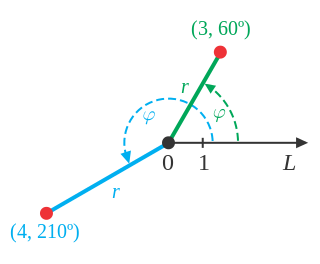
\includegraphics[height=5cm,keepaspectratio=true]{./trig/Examples_of_Polar_Coordinates.png}
		% Examples_of_Polar_Coordinates.svg.png: 0x0 pixel, 300dpi, 0.00x0.00 cm, bb=
	\end{center}
	

{}
	\begin{problema}
		Escriba los siguientes vectores en su forma polar (estándar):
		\begin{itemize}
			\item $\langle 1, \sqrt{3}\rangle$ 
			\item $\langle 1, -\sqrt{3}\rangle$ 
			\item $\langle -1, \sqrt{3}\rangle$ 
			\item $\langle -1, -\sqrt{3}\rangle$ 
		\end{itemize}
		
	\end{problema}
	

\subsection{Optimización}

	\begin{problema}
		\label{exe:0776}
		Suponga que en una sala de cine, una pantalla tiene 28 pies de alto. Cuando un espectador se sienta, la parte inferior de la pantalla tiene una altura de 6 pies por encima de su nivel de visión. El ángulo formado al dibujar una linea desde la parte inferior de la pantalla a la parte superior se conoce como ángulo de visión. Encuentre el ángulo máximo de visión respecto a la distancia al muro que sostiene la pantalla.
	\end{problema}


{}
	\begin{figure}[h]
		\centering
		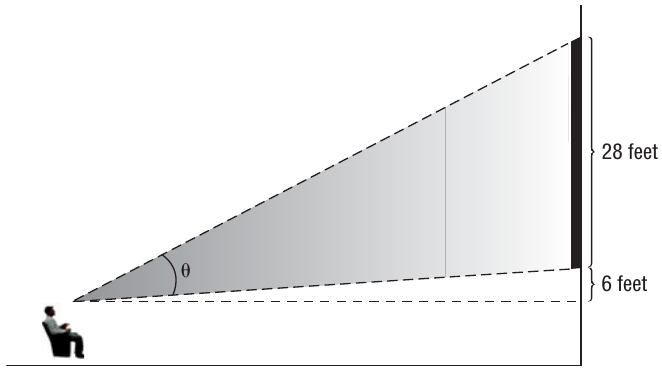
\includegraphics[width=10cm]{./trig/angulo_vision.png}
		% angulo_vision.png: 0x0 pixel, 300dpi, 0.00x0.00 cm, bb=
		\caption{Ángulo de visión}
		\label{fig:angulo_vision}
	\end{figure}
	

{Sugerencia}
	\begin{align*}
		\dfrac{d}{dx}\left( \tan^{-1}\left( \dfrac{A}{x} \right) \right)=
		-\dfrac{A}{A^{2}+x^{2}}
	\end{align*}



\section{Propiedades de funciones trigonométricas}

{}
	\begin{problema}
		\begin{itemize}
			\item Grafique cada una de las seis funciones trigonométricas en \texttt{Sagemath}.
			\item Determine el dominio y el rango de cada una.
		\end{itemize}  
	\end{problema}
	

{}
	\begin{definicion}
		Una función se llama periódica si existe un número positivo $p$ tal que siempre que $\theta$ esté en el dominio de $f,$ entonces $\theta+p$ lo está y 
		\begin{align*}
			f(\theta+p)=f(\theta).
		\end{align*}
		
		Si existe un número minimal $p$ con tal propiedad, diremos que este es el \emph{periodo fundamental} de $f.$
	\end{definicion}

{}
	\begin{problema}
		Determine el periodo respectivo de cada una de las seis funciones trigonométricas.
	\end{problema}
	


	\begin{problema}
		\label{exmp:6301}
		Encuentre el valor exacto de 
		\begin{itemize}
			\item $\sin\left( \dfrac{17\pi}{4} \right)$
			\item $\cos\left( 5\pi \right)$
			\item $\tan\left( \dfrac{5\pi}{4} \right)$
		\end{itemize}
		
	\end{problema}

{}
	\begin{figure}
		\centering
		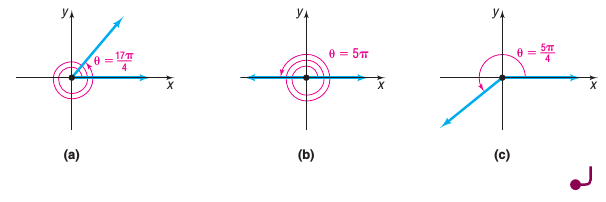
\includegraphics[width=11cm,keepaspectratio=true]{./trig/sull0628.png}
		% sull0628.png: 0x0 pixel, 300dpi, 0.00x0.00 cm, bb=
		\label{fig:0638}
	\end{figure}
	

{}
	\begin{problema}
		Determine el valor exacto de 
		\begin{itemize}
			\item $\sin(405^{o})$
			\item $\cot(390^{o})$
			\item $\sec\left( \dfrac{17\pi}{4} \right)$
		\end{itemize}
		
	\end{problema}
	

{Identidades reciprocas}
	\begin{align}
		\label{sull632}
		\csc(\theta)&= \dfrac{1}{\sin(\theta)}\\
		\sec(\theta)&= \dfrac{1}{\cos(\theta)}\\
		\cot(\theta)&= \dfrac{1}{\tan(\theta)}
	\end{align}

{}
	\begin{problema}
		\label{exmp:6303}
		Dado 
		\begin{align*}
			\sin(\theta)&= \dfrac{\sqrt{5}}{5}\\
			\cos(\theta)&= \dfrac{2\sqrt{5}}{5}
		\end{align*}
		encuentre el valor de las cuatro funciones trigonométricas restantes.
	\end{problema}
	

{}
	\begin{problema}
		\label{exe:6335}
		Dado 
		\begin{align*}
			\sin(\theta)&= -\dfrac{3}{5}\\
			\cos(\theta)&= \dfrac{4}{5}
		\end{align*}
		encuentre el valor de las cuatro funciones trigonométricas restantes.
	\end{problema}
	

{Identidades pitagóricas}
	\begin{align*}
		\sin^{2}\theta+\cos^{2}\theta=1
	\end{align*} 
	\begin{align*}
		\tan^{2}\theta + 1 = \sec^{2}\theta
	\end{align*} 
	\begin{align*}
		\cot^{2}\theta + 1 =\csc^{2}\theta
	\end{align*}


	La función coseno es par:
	$$ \cos(-x)=\cos(x) $$
	mientras que la función seno es impar:
	$$ \sin(-x)=-\sin(x) .$$

{}
	\begin{problema}
		\label{exmp:6304}
		Encuentre el valor exacto de cada expresión \emph{sin usar calculadora}:
		\begin{itemize}
			\item $\tan(20^{o})-\dfrac{\sin(20^{o})}{\cos(20^{o})}$ 
			\item $\sin^{2}\dfrac{\pi}{12}+\dfrac{1}{\sec^{2}\dfrac{\pi}{12}}$
		\end{itemize}
		
	\end{problema}
	

{}
	\begin{problema}
		Encuentre el valor exacto de cada expresión \emph{sin usar la calculadora}:
		\begin{itemize}
			\item $\sin(80^{o})\csc(80^{o})$
			\item $\cos(400^{o})\sec(40^{o})$
			\item $\dfrac{\sin(-20^{o})}{\cos(380^{o})}+\tan(200^{o})$
		\end{itemize}
		
	\end{problema}
	


	\begin{problema}
		\label{exmp:sull6305}
		Dado que $\sin\theta=\frac{1}{3}$ y $\cos\theta$, encuentre el valor exacto de cada una de las restantes cinco funciones trigonométricas.
	\end{problema}
	

{}
	\begin{figure}
		\centering
		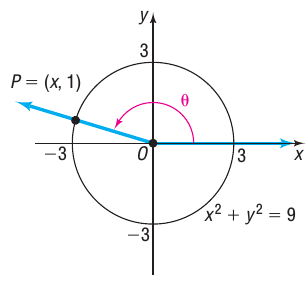
\includegraphics[height=8cm]{./trig/sull0641.png}
		% sull0641.png: 0x0 pixel, 300dpi, 0.00x0.00 cm, bb=
		\label{fig:0641}
	\end{figure}
	

{}
	

{}
	\begin{problema}
		Dado que $\tan\theta=\dfrac{1}{2}$ y $\sin\theta<0$, encuentre el valor exacto de cada una de las restantes cinco funciones trigonométricas en $\theta$.
	\end{problema}
	

{}
	\begin{figure}
		\centering
		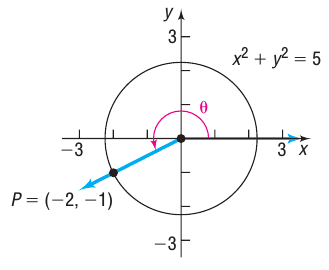
\includegraphics[height=8cm]{./trig/sull0642.png}
		% sull0641.png: 0x0 pixel, 300dpi, 0.00x0.00 cm, bb=
		\label{fig:0642}
	\end{figure}
	

{}
	\begin{problema}
		Encuentre el valor de cada una de las restantes funciones trigonométricas en $\theta$ conociendo que $\sin\theta=\dfrac{12}{13}$ y $\theta$ se encuentra en el segundo cuadrante.
	\end{problema}
	

{Paridad e imparidad}
	Por un lado, una función $f(\theta)$ es par si $f(-\theta)=f(\theta).$  Por otro lado, función $f(\theta)$ si $f(-\theta)=-f(\theta).$

{}
	\begin{figure}
		\centering
		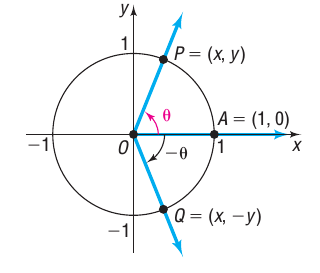
\includegraphics[height=8cm,keepaspectratio=true]{./trig/sull0443.png}
		% sull0443.png: 0x0 pixel, 300dpi, 0.00x0.00 cm, bb=
		\label{fig:0643}
	\end{figure}
	


	\begin{proposicion}
		La función $\cos$ es par, pero la función $\sin$ es par. 
	\end{proposicion}
	

{}
	\begin{problema}
		Determine si las funciones trigonométricas restantes son pares o impares.
	\end{problema}
	

{}
	\begin{problema}
		\label{exmp:0607}
		Encuentre el valor exacto de 
		\begin{itemize}
			\item $\sin(-45^{o})$ 
			\item $\cos(-\pi)$ 
			\item $\cot\left( -\dfrac{3\pi}{2} \right)$ 
			\item $\tan\left( -\dfrac{37\pi}{4} \right)$
		\end{itemize}
		
	\end{problema}
	

{}
	\begin{problema}
		\begin{itemize}
			\item $\sin(-60^{o})$
			\item $\csc(-30^{o})$
			\item $\cos\left( -\dfrac{\pi}{4} \right)$
			\item $\sec(-\pi)$
		\end{itemize}
		
	\end{problema}


\section{Suma y diferencias de ángulos}

{Suma y diferencias para el coseno}
	\begin{align*}
		\cos(s+t) &= \cos(s)\cos(t)-\sin(s)\sin(t) \\  
		\cos(s-t) &= \cos(s)\cos(t)+\sin(s)\sin(t)
	\end{align*}



	\begin{problema} Demuestre las siguientes identidades
		\begin{align*}
			\cos\left(\dfrac{\pi}{2}-t\right) &= \sin(t) \\
			\sin\left(\dfrac{\pi}{2}-t\right) &= \cos(t) 
		\end{align*}
	\end{problema}


{Suma y diferencias para el coseno}
	\begin{align*}
		\sin(s+t) &= \sin(s)\cos(t)+\cos(s)\sin(t) \\  
		\sin(s-t) &= \sin(s)\cos(t)-\cos(s)\sin(t)
	\end{align*}



	\begin{problema}
		Establezca la siguiente identidad
		\begin{align*}
			\dfrac{\cos\left(s-t\right)}{\sin(s)\sin(t)} 
			& = \cot(s)\cot(t)+1
		\end{align*}
	\end{problema}
	



	\begin{problema}
		Demuestre las siguientes identidades
		\begin{enumerate}
			\item $$ \tan(s+t)=\dfrac{\tan s + \tan t}{1- \tan s \tan t} $$ 
			\item $$ \tan(s-t)=\dfrac{\tan s - \tan t}{1+ \tan s \tan t} $$ 
			\item $$ \tan(s+\pi) = \tan(s) $$ 
			\item $$ \tan\left(s+\dfrac{\pi}{2}\right) = -\cot(s) $$
		\end{enumerate}
	\end{problema}



	\begin{problema}
		Demuestre las siguientes identidades
		\begin{enumerate}
			\item $$\sin\left(\dfrac{\pi}{2}+t\right) = \cos t$$
			\item $$\dfrac{\sin\left(s+t\right)}{\sin(s)\cos(t)} = 1+\cot(s)\tan(t)$$
		\end{enumerate}
	\end{problema}




\part{Álgebra Lineal}

\chapter{Sistemas lineales}

%402
\section{Sistemas de Ecuaciones Lineales Simultáneas}

\subsection{Sistemas de Dos Ecuaciones Lineales}

 Supongamos que $a_{i}, b_{i}, c_{i}, i=1,2$ son número dados:
	$$\begin{cases}
		a_{1}x+b_{1}y=c_{1}\\
		a_{2}x+b_{2}y=c_{2}\\
	\end{cases}
	$$
	En el sistema anterior, nuetro objetivos es encontrar dos números $x,y$ tales que cumplan ambas ecuaciones simultaneamente.



	\begin{problema}
		La soluci\'on del sistema 
		$$\begin{cases}
			x+y=7\\
			x-y=3
		\end{cases}
		$$ es $x=5,y=2.$
	\end{problema}
	



	A continuaci\'on, ejemplificaremos algunos de los m\'etodos más comunes para resolver sistemas de ecuaciones.

%

\begin{equation}
	\label{spi151}
	2x-y=4
\end{equation}
\begin{equation}	
	\label{spi152}
	x+2y=-3
\end{equation}		

	


{M\'etodo de sustituci\'on} 
	Despejando de \eqref{spi151}, obtenemos
	$$y=2x-4.$$
	
	Sutituyendo en \eqref{sp152}, obtenemos
	$$
	x+2(2x-4)=-3.
	$$
	


{M\'etodo de igualaci\'on}
	Despejando de \eqref{spi151}, obtenemos
	$$y=2x-4.$$
	
	Despejando de \eqref{sp152}, obtenemos
	$$y=-\dfrac{3+x}{2}.$$
	
	Igualando ambos lados derechos, obtenemos
	$$
	2x-4=-\dfrac{3+x}{2}.
	$$



{M\'etodo gráfico}
	\begin{figure}
		\centering
		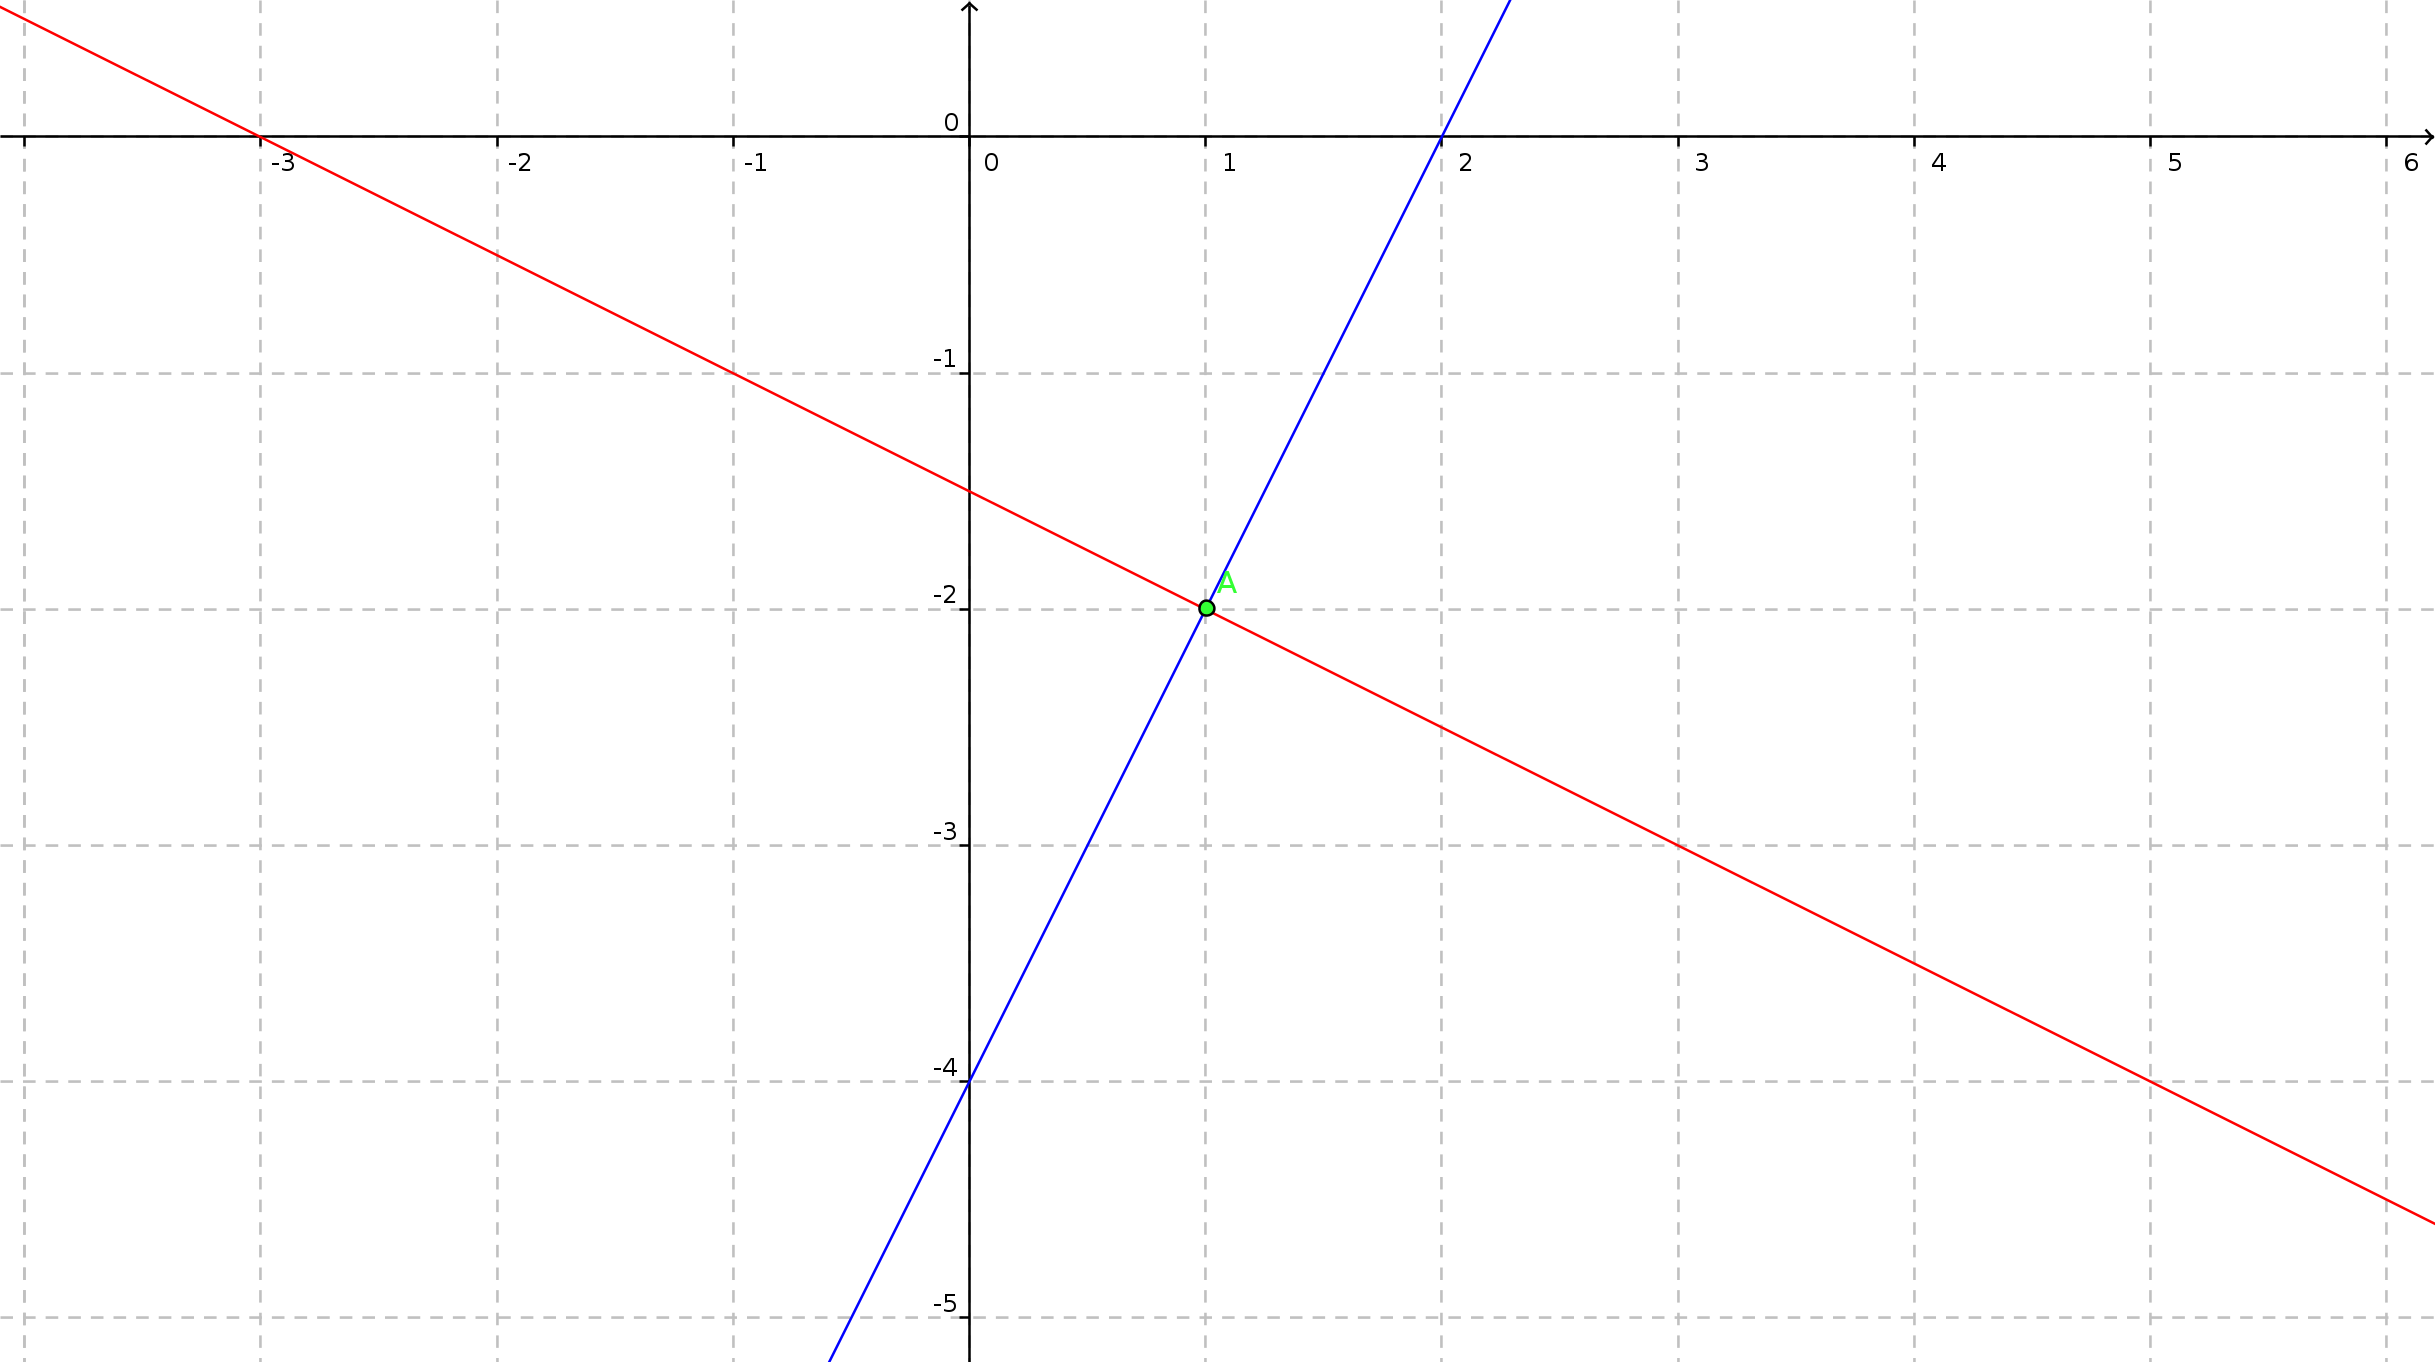
\includegraphics[height=5cm,keepaspectratio=true]{./precalculo/IM0401.png}
		% IM0401.png: 0x0 pixel, 300dpi, 0.00x0.00 cm, bb=
		\caption{$$2x-y=4\, , x+2y=-3$$}
		\label{fig:IM0401}
	\end{figure}
	


{Tipos de sistemas}
	\begin{figure}
		\centering
		\includegraphics[width=12cm,keepaspectratio=true]{./precalculo/IM0402.png}
		% IM0402.png: 0x0 pixel, 300dpi, 0.00x0.00 cm, bb=
		\label{fig:0401}
	\end{figure}
	



%403
\section{Determinantes}

\subsection{Determinantes de Segundo Orden}

{Definición}
	\begin{defn}
		$$
		\begin{vmatrix}
			a & b \\ c & d
		\end{vmatrix}=ad-bc.
		$$
	\end{defn}
	



	\begin{problema}
		$$
		\begin{vmatrix} 2 & 3 \\ -1 & -2 \end{vmatrix}=
		$$
	\end{problema}
	



	Si consideremos el siguiente sistema de ecuaciones
	\begin{equation}
		\begin{cases}
			a_{1}x+b_{1}y=c_{1}\\
			a_{2}x+b_{2}y=c_{2}
		\end{cases}...
	\end{equation}
	



	...y definimos
	\begin{align*}
		\Delta&=\begin{vmatrix} a_{1} & b_{1} \\ a_{2} & b_{2} \end{vmatrix}\\
		\Delta_{x}&=\begin{vmatrix} c_{1} & b_{1} \\ c_{2} & b_{2} \end{vmatrix}\\
		\Delta_{y}&=\begin{vmatrix} a_{1} & c_{1} \\ a_{2} & c_{2} \end{vmatrix}...
	\end{align*}



	...entonces
	\begin{equation}
		\label{spi:28.2}
		\begin{split}
			x&=\dfrac{\Delta_{x}}{\Delta}\\
			y&=\dfrac{\Delta_{y}}{\Delta}
		\end{split}
	\end{equation}
	



	\begin{problema}
		Resuelva el sistema
		$$\begin{cases}
			2x+3y=8\\
			x-2y=-3
		\end{cases}
		$$
	\end{problema}
	

\subsection{Ejemplos}


	El m\'etodo de soluci\'on de sistemas de ecuaciones linales, por medio de determinantes, se conoce como Regla de Cramer.



	\begin{problema} Resuelva el siguiente sistema por la Regla de Cramer
		\label{spi:28.4a}
		$$
		\begin{cases}
			4x+2y=5\\
			3x-4y=1
		\end{cases}
		$$
	\end{problema}
	



	\begin{problema} Resuelva el siguiente sistema por la Regla de Cramer
		\label{spi:28.4b}
		$$
		\begin{cases}
			3u+2v=18\\
			-5u-v=12
		\end{cases}
		$$
	\end{problema}
	


\subsection{Sistemas Indeterminados}


	Un sistema de $ n $ ecuaciones con $ n $ incognitas tiene una única solución si y solo si su determinante principal $ \Delta \neq 0. $  
	
	En este caso, decimos que el sistema es consistente.



	Si $ \Delta =0 $, entonces o bien existen multiples soluciones, o bien no existe alguna en absoluto.
	
	En cualquier caso, decimos que el sistema es inconsistente.



	Determine si 
	$$\begin{cases}
		5x-2y=10\\
		10x-4y=20
	\end{cases}$$
	es consistente; y de no ser el caso, explique que sucede con las soluciones.



	Determine si 
	$$\begin{cases}
		5x+3y=15\\
		10x+6y=60
	\end{cases}$$
	es consistente; y de no ser el caso, explique que sucede con las soluciones.




\subsection{Ejemplos}


	\begin{problema}
		\begin{align*}
			2x-y&=4\\
			x+y&=5
		\end{align*}
		
	\end{problema}
	



	\begin{problema}
		\begin{align*}
			5x+2y&=3\\
			2x+3y&=-1
		\end{align*}
		
	\end{problema}
	



	\begin{problema}
		\begin{align*}
			2x+3y=3\\
			6y-6x=1
		\end{align*}
		
	\end{problema}
	



	\begin{problema}
		\begin{align*}
			5y&=3-2x\\
			3x&=2y+1
		\end{align*}
		
	\end{problema}
	



	\begin{problema}
		\begin{align*}
			\dfrac{x-2}{3}+\dfrac{y+1}{6}=2\\
			\dfrac{x+3}{4}-\dfrac{2y-1}{2}=1
		\end{align*}
		
	\end{problema}
	


\section{Fracciones parciales}


 La técnica de fracciones parciales se utiliza para integrar funciones racionales, es decir, aquellas de la forma $$\dfrac{N(x)}{D(x)},$$ donde $N, D$ son polinomios.



 Por simplicidad, supondremos que
 \begin{enumerate}
  \item El coeficiente líder de $D(x)$ es igual a $1.$ 
  \item El grado de $D(x)$ es mayor que el de $N(x).$
 \end{enumerate}
 Sin embargo, ninguna de estas dos condiciones son esenciales.



 \begin{problema}
  \label{ayr:exmp:33.1}
  $$
    \int\dfrac{2x^{3}}{5x^{8}+3x-4}dx=
    \dfrac{1}{5}\int\dfrac{2x^{3}}{x^{8}+\frac{3}{5}x-\frac{4}{5}}
  $$
 \end{problema}




 \begin{problema}
  $$
  \dfrac{2x^{5}+7}{x^{2}+3}=2x^{3}-6x+\dfrac{18x+7}{x^{2}+3}
  $$
 \end{problema}




 \begin{definicion}
  Un polinomio es irreducible si no se puede expresar como el producto de dos polinomios de grado menor. 
 \end{definicion}




	\begin{enumerate}
		\item  Todo polinomio lineal es irreducible
		
		\item 
		Un polinomio cuadrático 
		$$g(x)=ax^{2}+bx+c, \, a\neq0$$ es irreducible si y solo $b^{4}-4ac<0.$
		
	\end{enumerate}



 \begin{problema}
  \label{ayr:exmp:33.3}
  Verifique que 
  \begin{enumerate}
   \item $x^{2}+4$ es irreducible;
   \item $x^{2}+x-4$ es reducible.
  \end{enumerate}

 \end{problema}




 \begin{teorema}
  \label{ayr:thm:33.1}
  Todo polinomio cuyo coeficiente líder sea igual a $1$ se puede expresar como producto de factores lineales, o factores cuadráticos irreducibles.
 \end{teorema}




 \begin{problema}
  \label{ayr:exmp:33.4}
  \begin{enumerate}
   \item $x^{3}-4x=$ 
   \item $x^{3}+4x=$ 
   \item $x^{4}-9=$ 
   \item $x^{3}-3x^{2}-x+3=$
  \end{enumerate}

 \end{problema}



\subsection{Método de Fracciones Parciales}


\subsection{Caso I. $D(x)$ es producto de factores lineales distintos}
 \begin{problema}
  \label{ayr:exmp:33.5}
  Resuelva $$\int \dfrac{dx}{x^{2}-4}$$
 \end{problema}




 \begin{problema}
  \label{ayr:exmp:33.6}
  Resuelva $$\int\dfrac{(x+1)dx}{x^{3}+x^{2}-6x}$$
 \end{problema}




\subsection{Regla General para Caso 1}
 El integrando se representa como una suma de términos de la form $\dfrac{A}{x-a},$ para cada factor $x-a,$ y $A$ una constante por determinar.



\subsection{Caso 2. $D(x)$ es producto de factores lineales repetidos.}
 \begin{problema}
  \label{ayr:exmp:33.7}
  Encuentre $$
  \int\dfrac{(3x+5)dx}{x^{3}-x^{2}-x+1}
  $$
 \end{problema}




 \begin{problema}
  \label{ayr:33.8}
  $$
  \int \dfrac{(x+1)dx}{x^{3}(x-2)^{2}}
  $$
 \end{problema}




\subsection{Regla General para el Caso 2.}
 Para cada factor $x-c$ de multiplicidad $k,$ se utiliza la expresión
 $$
 \dfrac{A_{1}}{x-r}+\dfrac{A_{2}}{(x-r)^{2}}+...+\dfrac{A_{k}}{(x-r)^{k}}.
 $$



\subsection{Caso 3. Factores cuadráticos irreducibles distintos, y lineales repetidos}
 A cada factor irreducible $x^{2}+bx+c$ de $D(x)$ le corresponde el integrando
 $$
 \dfrac{Ax+B}{x^{2}+bx+c}.
 $$



 \begin{problema}
  Encuentre $$
  \int \dfrac{(x-1)dx}{x(x^{2}+1)(x^{2}+2)}
  $$
 \end{problema}




\subsection{Caso IV. Factores cuadráticos irreducibles repetidos}
 
 A cada factor cuadráticos irreducible $x^{2}+bx+c$ de mutiplicidad $k$ le corresponde el integrando
 $$
 \sum_{i=1}^{k}\dfrac{A_{i}x+B_{i}}{(x^{2}+bx+c)^{i}}
 $$
 



 \begin{problema}
  Encuentre $$\int\dfrac{2x^{2}+3}{(x^{2}+1)^{2}}dx.$$
 \end{problema}



\section{Factores lineales sin repetición}

%%%%%%%%%%%%%%%%%%%%%
{}
\begin{problema}
Encuentre la expresión en fracciones parciales de
\begin{align}
	\dfrac{-29 \, x + 143}{2 \, x^{2} - 22 \, x + 56}
\end{align}
\end{problema}

\begin{align*}
	\dfrac{-29 \, x + 143}{2 \, x^{2} - 22 \, x + 56}= -\frac{9}{2 \, {\left(x - 4\right)}} - \frac{10}{x - 7}
\end{align*}


%%%%%%%%%%%%%%%%%%%%%
{}
	\begin{problema}
		Encuentre la expresión en fracciones parciales de
		\begin{align}
			\dfrac{-10 \, x - 30}{7 \, x^{2} + 4 \, x - 3}
		\end{align}
	\end{problema}
	
	\begin{align*}
		\dfrac{-10 \, x - 30}{7 \, x^{2} + 4 \, x - 3}= -\frac{24}{7 \, x - 3} + \frac{2}{x + 1}
	\end{align*}
	

%%%%%%%%%%%%%%%%%%%%%
{}
	\begin{problema}
		Encuentre la expresión en fracciones parciales de
		\begin{align}
			\dfrac{171 \, x + 175}{15 \, x^{2} + 38 \, x + 7}
		\end{align}
	\end{problema}
	
	\begin{align*}
		\dfrac{171 \, x + 175}{15 \, x^{2} + 38 \, x + 7}= \frac{22}{5 \, x + 1} + \frac{21}{3 \, x + 7}
	\end{align*}
	


\section{Factores lineales con repetición}

%%%%%%%%%%%%%%%%%%%%%
{}
	\begin{problema}
		Encuentre la expresión en fracciones parciales de
		\begin{align}
			\dfrac{-10 \, x + 109}{x^{2} - 20 \, x + 100}
		\end{align}
	\end{problema}
	
	\begin{align*}
		\dfrac{-10 \, x + 109}{x^{2} - 20 \, x + 100}= -\frac{10}{x - 10} + \frac{9}{{\left(x - 10\right)}^{2}}
	\end{align*}
	

%%%%%%%%%%%%%%%%%%%%%
{}
	\begin{problema}
		Encuentre la expresión en fracciones parciales de
		\begin{align}
			\dfrac{80 \, x + 31}{256 \, x^{2} + 96 \, x + 9}
		\end{align}
	\end{problema}
	
	\begin{align*}
		\dfrac{80 \, x + 31}{256 \, x^{2} + 96 \, x + 9}= \frac{5}{16 \, x + 3} + \frac{16}{{\left(16 \, x + 3\right)}^{2}}
	\end{align*}
	

%%%%%%%%%%%%%%%%%%%%%
{}
	\begin{problema}
		Encuentre la expresión en fracciones parciales de
		\begin{align}
			\dfrac{30 \, x - 14}{25 \, x^{2} - 20 \, x + 4}
		\end{align}
	\end{problema}
	
	\begin{align*}
		\dfrac{30 \, x - 14}{25 \, x^{2} - 20 \, x + 4}= \frac{6}{5 \, x - 2} - \frac{2}{{\left(5 \, x - 2\right)}^{2}}
	\end{align*}
	



\chapter{Espacios Vectoriales}
\section{Definici\'on y ejemplos}



Hasta ahora hemos considerado a los vectores como elementos de un espacio $$\R^{n}=\set{(x_{1},...,x_{n}|x_{k}\in\R)},$$ por ejemplo vectores en el plano $\R^{2}=\set{(x,y)|x,y\in \R}$ o en el espacio $\R^{3}=\set{(x,y,z)|x,y,z\in \R}.$ En cada caso, ten\'iamos una suma entre vectores y una multiplicaci\'on por \emph{escalares,} es decir, número reales.

\begin{problema}
 Si ${u}=(u_{1},u_{2})$ y ${v}=(v_{1},v_{2})$ son vectores en $\R^{2},$ y $\a \in \R,$ entonces $$(u_{1},u_{2})+(v_{1},v_{2})=(u_{1}+v_{1},u_{2}+v_{2}),$$ mientras que $$\a(u_{1},u_{2})=(\a u_{1},\a u_{2}).$$


 En este caso, la suma tiene las siguientes propiedades:
 \begin{enumerate}
  \item(Cerradura)  ${u}+{v}=(u_{1},u_{2})+(v_{1},v_{2})=(u_{1}+v_{1},u_{2}+v_{2}),$ es un vector en $\R^{2},$
  \item(Asociatividad) Si $w=(w_{1},w_{2})$ es otro vector en $\R^{2},$ entonces
  \begin{align*}
(u+v)+w&=\left( (u_{1},u_{2})+(v_{1},v_{2}) \right) + (w_{1},w_{2}) \\
&=(u_{1},u_{2}) + \left( (v_{1},v_{2}) + (w_{1},w_{2}) \right) \\
&=u+(v+w),
  \end{align*}
\item(Conmutatividad)
$
u+v=(u_{1}+v_{1},u_{2}+v_{2})=(v_{1}+u_{1},v_{2}+u_{2})=v+u
$
\item(Existencia de un elemento neutro)
$
u+\vec{0}=(u_{1},u_{2})+(0,0)=(u_{1},u_{2})=u,
$
y de la misma forma $\vec{0}+u=u.$
\item(Inversos aditivos) Para $u=(u_{1},u_{2}),$ definimos $$-u=(-u_{1},-u_{2}),$$ y este elemento satisface que
$$
u+(-u)=(-u)+u=0.
$$
 \end{enumerate}


 La multiplicaci\'on por escalares satisface las siguientes  propiedades
 \begin{enumerate}
 \item $\a u$ es de nuevo un vector en $\R^{2},$
  \item $1u=1(u_{1},u_{2})=(1\cdot u_{1},1\cdot u_{2})=u,$
  \item $(\a\b) u=\a(\b u_{1}, \b u_{2})=\a(\b u).$
 \end{enumerate}

 Finalmente, la suma de vectores y la multiplicaci\'on por escalares estan relacionadas por las siguiente leyes distributivas.
 \begin{enumerate}
  \item $(\a+\b)u=((\a+\b)u_{1},(\a+\b)u_{2})=(\a u_{1},\a u_{2})+(\b u_{1},\b u_{2})=\a u +\b u,$
  \item $\a(u+v)=\a(u_{1}+v_{1},u_{2}+v_{2})=(\a(u_{1}+v_{1}),\a(u_{2}+v_{2}))=\a(u_{1},u_{2})+\a(v_{1},v_{2})=\a u +\a v.$
 \end{enumerate}
\end{problema}

\begin{problema}[\dag]
 Verificar que las mismas propiedades se cumplen para $\R^{3},$ usando la suma de vectores y multiplicaci\'on por
escalares conocida.
\end{problema}

Estas propiedades se cumplen para muchos y muy diferentes conjuntos, donde tenemos una operaci\'on suma entre sus elementos y podemos definir una multiplicaci\'on por números reales. De hecho, estos conjuntos son los objetos de estudio en el álgebra lineal.

\begin{defn}
 Sea $V$ un conjunto, con una operaci\'on $+:V \times V \to V$ y una operaci\'on $\cdot:\R \times V \to V.$ Decimos
que $V$ es un \emph{espacio vectorial (sobre $\R$)} si para todo $u,v,w\in V$ y $\a,\b\in \R$ se cumplen las siguientes
propiedades.
 \begin{enumerate}
  \item(Cerradura)$u+v\in V,$
  \item(Asociatividad)$(u+v)+w=u+(v+w),$
  \item(Conmutatividad)$u+v=v+u,$
  \item(Elemento neutro) Existe $0\in V,$ tal que para todo $u\in V: u+0=0+u=u,$
  \item(Elementos inversos) Para todo $u\in V,$ existe $-u \in V,$ tal que $u+(-u)=(-u)+u=0.$
  \item $\a u \in V,$
 \item $1u=u,$
 \item $(\a\b)u=\a(\b u),$
\item $(\a+\b)u=\a u+\b u,$
\item $\a(u,v)=\a u + \a v.$
\end{enumerate}

A los elementos del espacio vectorial $V$ les llamamos \emph{vectores.}
\end{defn}

\begin{rem}
 Cuando $V$ es un espacio vectorial, con operaci\'on suma $+:V \times V \to V$ y multiplicaci\'on por escalares
$\cdot:\R \to V \to V,$ por brevedad, decimos que $(V, +, \cdot)$ es un espacio vectorial.
\end{rem}



\subsection*{Ejemplos}

%Para resolver los ejercicios de esta secci\'on puede consultar \cite[sec. 4.2]{G} y \cite[sec. 2.1]{HK}.

\begin{problema}[\dag]
Demuestre usando las propiedades anteriores, que en cualquier espacio vectorial se cumplen las siguientes propiedades.
\begin{enumerate}
 \item $0  u=\a  0=0.$ (Note que el cero escrito a la izquierda denota el cero como número, mientras que escrito a la izquierda o solo, denota el elemento neutro  del espacio vectorial.)
 \item $-u=(-1) u.$ \emph{Sugerencia: Verifique que $u+(-1)u=0$.}
 \item Si $\a u=0,$ entonces o bien $\a=0$ o $u=0.$
 \item El elemento neutro $0$ es único.
 \item Para cada vector $u,$ su inverso aditivo $-u$ es único.
\end{enumerate}
\end{problema}

\begin{problema}
 Compruebe que los siguientes conjuntos son espacios vectoriales (reales), con las operaciones suma y multiplicaci\'on por escalar usuales.
 \begin{enumerate}
 \item $\set{0}.$
 \item $\set{(x,y)\in \R^{2}|y=mx}$ para $m\in \R$ fijo.
 \item $\set{(x,y,z)\in \R^{3}| ax+by+cz=0}$ para $a,b,c\in \R.$
 \item $\set{(x,y,z)\in \R^{3}|(a,b,c)\cdot (x,y,z)=0}$ para $a,b,c\in \R.$
  \item $\set{f|f:S\to \R},$ donde $S$ puede ser cualquier conjunto fijos.
  \item $\R^{m\times n},$ es decir, el conjunto de matrices $m\times n$ con entradas reales.
  \item  El espacio de polin\'omios con coeficientes reales.
  \item El espacio de polin\'omios con coeficientes reales de grado $\leq n,$ para $n \in \N$ fijo.
  \item $C[a,b],$ el espacio de funciones continuas en el intervalo $[a,b].$
  \item El conjunto de número reales \emph{positivos} con las operaciones $u\oplus v:= u,v$ y $\a \cdot u:=u^{\a}.$
 \end{enumerate}
\end{problema}

% \begin{problema}
%  Indique si los siguientes conjuntos son espacios vectoriales
%  \begin{enumerate}
%   \item El conjunto de matrices diagonales $2 \times 2,$ bajo la multiplicaci\'on, es decur, con la suma definida como $A\oplus B=AB.$
%   \item Los vectores en el primer cuadrante del plano.
%   \item $\set{(x,y)|y\geq 0}$
%   \item El conjunto de vectores en $\R^{3}$ de la forma $(x,x,x).$
%   \item El conjunto de matrices $2\times 2$ de la forma
%   $$
% \begin{pmatrix}
%  0 & -a\\
%  a & a\\
% \end{pmatrix}
%   $$
% \item El conjunto de funciones continuas de valores reales definidas en $[0,1]$  con $f(0)=f(1)=0.$
% \item $R^{2}$ con la suma definida como $$(x_{1},y_{1})\oplus (x_{2},y_{2})=(x_{1}+x_{2}+1, y_{1}+y_{2}+1),$$ y la multiplicaci\'on usual por escalares.
% \item El conjunto de funciones diferenciables en $[0,1]$ con las operaciones usuales.
% \item El conjunto de números reales de la forma $a+b\sqrt{2},$ donde $a,b$ son números racionales, bajo la suma usual y la multiplicaci\'on por escalares restringida a número racionales
% \item $\R^{2}$ con la suma usual y la multiplicaci\'on por escalares definida como $\a\cdot u=(\a u_{1},u_{2}).$
% \item $\R^{2}$ con las suma definida como
% $$
% u \oplus v:= u-v,
% $$
% y la multiplicaci\'on por escalares como
% $$
% \a \cdot u := -\a u.
% $$
% \item $\R^{2}$ con las suma definida como
% $$
% u \oplus v:= (u_{1}+v_{1},0),
% $$
% y la multiplicaci\'on por escalares como
% $$
% \a \cdot u := (\a u_{1},0).
% $$
% \end{enumerate}
% \end{problema}

\begin{problema}
 Considere la ecuaci\'on diferencial de segundo orden homog\'enea
 $$
y''(x)+a(x)y'+b(x)y(x)=0
 $$
donde $a,b$ son funciones continuas. Demuestre que el conjunto de soluciones de la ecuaci\'on diferencial es un espacio vectorial bajo las reglas usuales para la suma de funciones y multiplicaci\'on por escalares.
 \end{problema}






\section{Subespacios vectoriales}



\begin{problema}
 $\R^{2}$ es un espacio vectorial con las operaciones $$(u_{1},u_{2})+(v_{1},v_{2})=(u_{1}+v_{1},u_{2}+v_{2})$$ y
$$\a(u_{1}, u_{2})=(\a u_{1}, \a u_{2}).$$

En la secci\'on anterior consideramos el subjunto $$L_{c}=\set{(u_{1},u_{2})|u_{2}=c u_{1}}\subset \R^{2}$$ para  $c$
una pendiente fija, y verificamos que en efecto, con las mismas operaciones es un espacio vectorial.

Decimos entonces que $L_{c}$ es un subespacio vectorial de $\R^{2}.$
\end{problema}

\begin{defn}
 Si $(V, +, \cdot )$ es un espacio vectorial  y
$W\subset V$ es tambi\'en espacio vectorial, con las mismas operaciones $+,\cdot$ decirmos que $W$ es un subespacio
vectorial de $V,$ y podemos escribir $W < V.$
\end{defn}

En principio, si $W < V$, tendr\'iamos que verificar todos loa axiomas de espacio vectorial para $(W, +, \cdot).$ Sin
embargo, si en el espacio $V,$ la suma es asociativa y conmutativa, tambi\'en lo será en $W.$ De igual manera, el
elemento neutro $1\in V$ de la multiplicaci\'on por escalares es el mismo en $W,$ y se sigue cumpliendo la
asociatividad de la multiplicaci\'on por escalares y las leyes de distribuci\'on.

Entonces, basta demostrar que se cumplen los restantes axiomas, a saber:
\begin{enumerate}
 \item Si $u,v \in W,$ entonces $u+v\in W.$
 \item Si $\a \in \R, v \in W,$ entonces $\a v\in W.$
 \item $0\in W.$
 \item Si $u\in W,$ entonces $-u\in W.$
\end{enumerate}

Sin embargo, los dos últimos incisos se siguen del segundo. En efecto, si escogemos $\a=0$ y cualquier $u\in
W,$ entonces
$$
0=0\cdot u \in W.
$$
De igual manera, para cualquier $u\in W,$ si escogemos $\a=-1,$ entonces $-u=(-1)u\in W.$

Por último, verificar los dos axiomas restantes es equivalente a verificar que para todo $\a \in \R, u,v \in W,$
$$
\a u + v \in W.
$$

\begin{prop}
 Si $W\subset V,$ entonces $$
W < V \iff \forall \a \in \R, u,v \in W, \a u+v\in W.
 $$
\end{prop}

\begin{cor}
 Todo $W < V$ contiene a $0 \in V.$
\end{cor}


\begin{defn}
 Si $W< V,$ pero $W\neq\set{0}$ y $W\neq V,$ entonces decimos que $W$ es un subespacio (vectorial) propio.
\end{defn}

\begin{defn}
 Sean $u,v_{1},...,v_{k}$ vectores en un espacio vectorial $V.$ Decimos que $u$ es combinaci\'on lineal de
$v_{1},...,v_{k}$ si existen escalares $\a_{1},...,\a_{k}\in \R$ tales que:
$$
u=\a_{1}v_{1}+...\a_{k}v_{k}.
$$
\end{defn}

\begin{defn}
 Sea $V$ un espacio vectorial. El subespacio generado por un subconjunto $S=\set{v_{1},...,v_{k}}\subset V$ se define
como
 $$
\gen{S}=\set{\a_{1}v_{k},...,\a_{k}v_{k}\av \a_{1},...,\a_{k}\in \R},
 $$
 es decir, el conjunto de todas las combinaciones lineales de $v_{1},...,v_{k}.$
\end{defn}

\begin{rem}
 $\gen{S}<V.$
\end{rem}


\begin{problema}
 $u=(2,0,2)$ es combinaci\'on lineal de $v_{1}=(1,0,1)$ y $v_{2}=(0,1,1)$ porque $u=2v_{1}-v_{2}.$

 De hecho, $$\gen{v_{1},v_{2}}=\set{(a,b,a+b)\av a,b \in \R}<\R^{3}$$ es el plano que contiene a estos dos vectores.

 $(-1,-1,1)\notin \gen{v_{1},v_{2}},$ porque no vive en este plano.
\end{problema}





\subsection*{Ejemplos}

Los siguientes ejercicios se pueden encontrar en \cite[sec. 4.3]{G} y \cite[sec. 2.2]{HK}.

% \begin{problema} En los siguientes ejercicios, verificar que $W < V,$ con las operaciones $+,\cdot$ usuales en $V.$
% Justifique su respuesta.
%  \begin{enumerate}
%   \item $V=\R^{2}, W=\set{(x,y)|ax+by=0},$ con $a,b\in \R$ fijos
%   \item $V=\R^{3}, W=\set{(at,bt,ct)|t\in \R},$ con $a,b,c\in \R$ fijos
%   \item $V=\R^{3}, W=\set{(a,y,z)|ax+by+cz=0},$ con $a,b,c\in \R$ fijos
%   \item $V=P_{n}, W=P_{m},$ donde $P_{k}$ es el espacio de polinomios (con coeficientes reales) de grado menor
% o igual a $k$ y $n\geq m.$
% \item $V=M_{mn}, W=\set{(a_{ij})\in M_{mn}|a_{11}=0}$
% \item $V=C[0,1], W=P_{n}[0,1],$ donde $P_{k}$ es el espacio de polinomios (con coeficientes reales) de grado
% menor o igual a $k$ restringidos al intervalo $[0,1].$
% \item $V=C[0,1], W=\set{f\in V|\int_{0}^{1}f(x)dx=0}$
% 
%  \end{enumerate}
% \end{problema}

\begin{problema}
 ¿Cuál de los siguientes conjuntos de vectores $$u=(u_{1},u_{2},u_{3})$$ en $\R^{3}$ son subespacios de $\R^{3}$?
 \begin{enumerate}
  \item $\set{u\av u_{1}\geq 0}$
  \item $\set{u\av u_{1}+3u_{2}=u_{3}}$
  \item $\set{u\av u_{2}=u_{1}^{2}}$
  \item $\set{u\av u_{1}u_{2}=0}$
  \item $\set{u\av a_{2}\text{ es racional}}$
 \end{enumerate}

\end{problema}

\begin{problema}
 Sea $V$ el espacio vectorial (real) de todas las funciones $f:\R \to \R.$ ¿Cuales de los siguientes conjuntos son
subespacios de V?
\begin{enumerate}
 \item todas las funciones $f$ tales que $f(x^{2})=f^{2}(x)$
 \item todas las funciones $f$ tales que $f(0)=f(1)$
 \item todas las funciones $f$ tales que $f(3)=1+f(-5)$
 \item todas las funciones $f$ tales que $f(-1)=0$
\end{enumerate}

\end{problema}

% \begin{problema} ¿Es cierto que
% $$(3,-1,0,-1)\in \gen{(2,-1,3,2), (-1,1,1,-1), (1,1,9,-5)}$$?
% \end{problema}

\begin{problema}
 Sea $W$ el conjunto de todos los vectores $(x_{1},...,x_{5})$ que satisfacen
 \begin{align*}
  2x_{1}-x_{2}+\frac{4}{3}x_{3}-x_{4}&=0 \\
  x_{1}+\frac{2}{3}x_{3}-x_{5}&=0 \\
  9x_{1}-3x_{2}+6x_{3}-3x_{4}-3x_{5}&=0.
 \end{align*}
Mostrar que $W$ es subespacio vectorial de $\R^{5}.$
\end{problema}



\begin{problema}[\dag]
\begin{enumerate}
   \item  Verificar que si $U,W < V,$ entonces $U\cap W < V.$
   \item Demostrar que si $U=\set{u_{1},...,u_{m}}$ y $W=\set{w_{1},...,w_{m}},$ entonces
   $$
U\cap W = \gen{u_{1},...,u_{n},w_{1},...,w_{m}}.
   $$
\end{enumerate}


\end{problema}

% \begin{problema}
%  En los siguientes ejercicios, verificar \emph{si} $W < V,$ con las operaciones $+,\cdot$ usuales en $V.$
% Justifique su respuesta.
% \begin{enumerate}
% \item $V=M_{nn}, W=\set{A\in M_{nn}|A\text{ es invertible}}$
% \item $V=M_{nn}, W=\set{A\in M_{nn}|A\text{ no es invertible}}$
% \item $V=M_{nn}, W=\set{A\in M_{nn}|AB=BA}$ para alguna matriz $B\in M_{nn}$ fija.
% \item $V=M_{nn}, W=\set{A\in M_{nn}|A^{2}=A}$
% \item $V=M_{nn}, W=\set{A\in M_{nn}|A\text{ es diagonal}}$ \footnote{Consulte \cite[pag. 114]{G}}
% \item $V=M_{nn}, W=\set{A\in M_{nn}|A\text{ es triangular}}$ \footnote{Consulte \cite[pag. 88]{G}}
% \item $V=M_{nn}, W=\set{A\in M_{nn}|A\text{ es simetrica}}$ \footnote{Consulte \cite[pag. 123]{G}}
%  \item $V=C^{1}[0,1], W=\set{f\in C^{1}[0,1]|f'(0)=0}$
%  \item $V=C[a,b], W=\set{f\in C[a,b]| \int_{a}^{b}f(x)dx=0}$
%  \item $V=C[a,b], W=\set{f\in C[a,b]| \int_{a}^{b}f(x)dx=0}$
%  \end{enumerate}
% 
% 
% \end{problema}


\begin{problema}[\dag]
\begin{itemize}
 \item Sean $u,v \in \R^{2}.$ Mostrar que $$W=\set{\a u+ \b v| \a, \b \in \R} < \R^{2}.$$
 \item Mostrar que si $u,v$ no son paralelos, entonces para cualquier $w\in \R^{2},$ podemos encontrar $\a,\b \in
\R$ de manera que $w= \a u + \b v.$
\end{itemize}
\end{problema}

\begin{problema}[\dag]
 Sea $A$ una matriz $m\times n$ con entradas reales. Demostrar que el conjunto de todas los vectores columna $u$ de
longitud $n,$ tales que $Au=0$ es un subespacio vectorial de todos los vectores columna $\R^{n}.$
\end{problema}

\section{Transformaciones lineales}

\subsection*{Definici\'on y ejemplos}
\begin{definicion} Sean $V,W$ espacios vectoriales. Decimos que $T:V \to W$ es una \emph{transformaci\'on lineal} si para
todos $\a \in \R, u,v \in V$ se cumple
\begin{enumerate}
\item $T(u+v)=T(u)+T(v)$ ($T$ abre sumas)
 \item $T(\a u)=\a T(u)$ ($T$ saca escalares)
\end{enumerate}
o de manera equivalente
$$
T(\a u +v)=\a T(u) + T(v),
$$
es decir, \emph{$T$ respeta la estructura de espacio vectorial.}

En el caso $V=W,$ decimos que $T:V\to V$ es un operador y al conjunto de operadores en $V$ lo denotamos por $L(V).$
En el caso $W=\R,$ decimos que $T:V\to \R$ es un funcional en $V.$
\end{definicion}

\begin{problema}
 Sea $a=[a_{1},...,a_{n}]\in \R^{n}$ fijo y definamos $T:\R^{n}\to \R, \, T(u)=a \cdot u.$ Entonces, $T$ es una
transformaci\'on lineal. 
\end{problema}


\begin{problema}
\label{matriz:trans_lin}
Sea $A=\begin{bmatrix}
        a_{ij}
       \end{bmatrix}
$ una matriz de dimensi\'on $n \times m,$ donde $n$ indica el número  de columnas y $m$ el de renglones.

Si definimos $T:\R^{n}\to \R^{m}, \, T(u)=Au,$ entonces $T$ es una tranformaci\'on lineal. En otras palabras, cada
matriz define una transformaci\'on lineal. Lo inverso tambi\'en es cierto.

Sea $$e_{k}=\begin{bmatrix}
             0\\
             \vdots \\
             1 \\
             \vdots \\
             0             
            \end{bmatrix}
$$
el vector columna con un $1$ en la $k-$\'esima posici\'on y ceros en el resto, y sea $T:\R^{n}\to \R^{m}$ una
transformaci\'on lineal. Entonces, $T(e_{k})\in \R^{m}$ y digamos que es de la forma
$$
T(e_{k})=\begin{bmatrix}
          a_{1k}\\
          \vdots \\     
          a_{mk} \\
         \end{bmatrix}.
$$

Si definimos $A=[a_{ij}]\in M_{mn}$ entonces $T(e_{k})=Ae_{k}, \, k=1,...,n.$ Por linealidad tanto de $T$ como de $A,$
obtenemos que $T(x)=Ax,$ para todo vector $x\in \R^{n}.$
\end{problema}

\begin{problema}
Las siguientes transformaciones son lineales:
\begin{itemize}
 \item $T:C^{1}[0,1]\to C^{0}[0,1],$
 $$
T(f)(x)=f'(x).
 $$
 \item $T:C^{0}[0,1]\to \R,$
$$
T(f)=\int_{0}^{1}f(t)dt.
$$
\item $T:C^{0}[0,1]\to C^{1}[0,1],$
$$
T(f)(x)=C+\int_{0}^{x}f(t)dt, 
$$
donde $x\in[0,1]$ y $C\in \R$ es alguna constante.
\end{itemize}

\end{problema}

\begin{problema}
 Indique si la siguiente transformaci\'on $T:\R^{3}\to \R^{3}$ es lineal y de ser as\'i, encuentre su representaci\'on
matricial.
\[
\label{trans_exmp}
 T\begin{bmatrix}
    x\\y\\z
   \end{bmatrix}=
   \begin{bmatrix}
    x+2y \\ z-y\\ 2x+7y-3z
   \end{bmatrix}
\]

\end{problema}

\begin{solucion}
 La prueba de que la transformaci\'on es lineal se deja al lector. Ahora bien,
 $$
T\begin{bmatrix}
  1\\0\\0
 \end{bmatrix}
=\begin{bmatrix}
  1\\0\\2
 \end{bmatrix},
 T\begin{bmatrix}
  0\\1\\0
 \end{bmatrix}
=\begin{bmatrix}
  2\\-1\\7
 \end{bmatrix},
T\begin{bmatrix}
  0\\0\\1
 \end{bmatrix}
=\begin{bmatrix}
  0\\1\\-3
 \end{bmatrix}.
 $$

 Por lo tanto, la representaci\'on matricial de $T$ esta dada por
 $$
=\begin{bmatrix}
1 & 2 & 0 \\
0 & -1 & 1 \\
2 & 7 & -3
 \end{bmatrix}
 $$
\end{solucion}


\subsection*{Operadores en  $\R^{n}$}

Sean $T,S \in L(\R^{n}).$ La composici\'on $TS,$ es decir, $TS(x)=T(S(x))$ es de nuevo un operador y de hecho, si 
$B=[b_{ij}]$ es la matriz asociada a $T$ como en el ejemplo \ref{matriz:trans_lin} y $A=[A_{ij}]$ la asociada a $S,$
entonces la matriz asociada a $TS$ es $C=[c_{ij}]$ conjunto $$
c_{ij}=\sum_{k}^{n}b_{ik}a_{kj}.
$$
Decimos que $C=BA$ es el producto de de $B$ con $A$ (es este orden), y esta composicion es asociativa.

El operador de $T$ con $S$ suma esta definido como $(T+S)(u)=T(u)+S(u),$ y de hecho tiene asociada la matriz $$
\begin{bmatrix}
 b_{ij}+a_{ij}
\end{bmatrix}.
$$

Dos operadores especiales en $R^{n}$ son la \emph{transformaci\'on cero} $0(x)=0$ y la \emph{identidad} $\id(x)=x.$
\begin{problema}[\dag]
 Encuentre la matriz asociada a los operadores cero e identidad. 
\end{problema}

Podemos definir la multiplicaci\'on de operadores por escalares de la siguiente forma. $(\a T)(u)=\a T(u).$ De esta
manera, con la operaci\'on suma entre operadores y esta multiplicaci\'on por escalares, resulta que $L(\R^{n})$ es un
espacio vectorial.

Finalmente, si para $P\in L(\R^{n})$ existe $Q\in L(\R^{n}),$ de manera que $PQ=\id,$ decimos que $P$ es
\emph{invertible} y que $Q$ es el operador inverso de $P.$ Tambi\'en podemos escribir $Q$ como $P^{-1}.$
De hecho, si $A$ es la matriz asociada a $P,$ entonces $A^{-1}$ es la asociada a $P^{-1}.$




\subsection*{Ejemplos}

\begin{problema} \label{exe:trans}Verificar que las siguientes transformaciones son lineales, y encontrar la representaci\'on
matricial de cada una.
\begin{enumerate}
 \item (Proyecci\'on sobre el plano)$$
T\begin{bmatrix}
  x \\ y \\z
 \end{bmatrix}
=\begin{bmatrix}
  x \\ y \\0
 \end{bmatrix}
 $$

 \item $$
T\begin{bmatrix}
  x \\ y \\z 
 \end{bmatrix}
 =\begin{bmatrix}
  x - y\\ y+z \\ 2x - y - z \\ -x+y+2z
 \end{bmatrix}
 $$

 \item $$
T\begin{bmatrix}
  x \\ y \\z
 \end{bmatrix}
 =\begin{bmatrix}
  2x - y +3z\\ 4x-2y+6z \\ -6x +3 y - 9z
 \end{bmatrix}
 $$

\item$$
T\begin{bmatrix}
  x \\ y 
 \end{bmatrix}
 =\begin{bmatrix}
   2x-y\\ 2y-4x
  \end{bmatrix}
$$

\item$$
T\begin{bmatrix}
  x \\ y 
 \end{bmatrix}
 =\begin{bmatrix}
   2x \\ 3x-y
  \end{bmatrix}
$$

\item$$
T\begin{bmatrix}
  x \\ y \\z
 \end{bmatrix}
 =\begin{bmatrix}
   2x-y+3z \\ 6x -3y +9z
  \end{bmatrix}
$$

\item $$
T\begin{bmatrix}
  x \\ y 
 \end{bmatrix}
 =\begin{bmatrix}
2x+y \\ 2y-x \\ x+8y
  \end{bmatrix}
$$
\item
$$
T\begin{bmatrix}
  x\\y\\z
 \end{bmatrix}
=\begin{bmatrix}
  1x  -3z \\
   -y + 5z
 \end{bmatrix}
$$
\item
$$
T\begin{bmatrix}
  x \\ y
 \end{bmatrix}
=\begin{bmatrix}
  2x+y\\
  -4x + 2y \\
  8x + 4y
 \end{bmatrix}
$$
\item
$$
T=\begin{bmatrix}
   x\\y\\z
  \end{bmatrix}
=\begin{bmatrix}
  3x  -z \\
  -y + 2z \\
  15x  -2y  -z
 \end{bmatrix}
$$

%  \item(Rotaci\'on en el plano)$$
% T \begin{bmatrix}
%    r\cos(t) \\
%    r\sin(t)
%   \end{bmatrix}
% = \begin{bmatrix}
%    r\cos(t+a) \\
%    r\sin(t+a)
%   \end{bmatrix}
%  $$

%  \item $T:P_{2} \to P_{3}, (Tp)(x)=xp(x).$
% 
%  \item $T:P_{3} \to P_{2}, T(a+bx+cx^{2}+dx^{3})=b+cx^{2}.$
\end{enumerate}
\end{problema}

\begin{problema}
 Encuentre una expresi\'on matemática para la transformaci\'on que rota un vector en el plano, con un ángulo $\phi$
en el sentido positivo (contrario a las manecillas del reloj). Indique si esta transformaci\'on es lineal y de serlo,
encuentre su representaci\'on matricial. \emph{Sugerencia: Exprese el vector en coordenadas polares.}
\end{problema}

\section{Núcleo e imagen}


\begin{defn}
 El \emph{núcleo} de una transformaci\'on lineal $T:V\to W,$ donde $V$ y $W$ son espacios vectoriales, es el
conjunto
$$
\ker(T)=\set{v\in V | T(v)=0}.
$$

La imágen de $T:V \to W$ es el conjunto
$$
\Im(T)=\set{w\in W | \exists v\in V, T(v)=w}.
$$
\end{defn}

\begin{prop}
$\ker(T) < V, \Im(T)<W.$
\end{prop}

\begin{proof}
 Si $\a\in \R$ y $u,v \in \ker(T),$ entonces
 \begin{align*}
  T(\a u +v) &= \a T(u) + T(v) & \text{(Por linealidad de $T$)} \\
  &= \a 0 + 0 & \text{(Porque $T(u)=T(v)=0$)} \\
  &= 0 &
 \end{align*}
Por tanto, $\ker(T)<V.$

Ahora, si $\a\in \R$ y $w,w' \in \Im(T),$ entonces Existen $v,v'\in V$ tales que $T(v)=w, T(w')=v'.$ Por lo cual, 
\begin{align*}
 \a w + w' &= \a T(v) + T(v') \\
 &= T(\a v + v').
\end{align*}
Como $\a v + v' \in V,$ entonces $\a w + w' \in W.$
\end{proof}

\begin{problema}
\label{texmp:ker}
 Encontrar un conjunto de vectores que generen $\ker(T),$ para la tranformaci\'on lineal $T$ dada por
(\ref{trans_exmp}).
\end{problema}

\begin{solucion}
 Supongamos que
 $$
 T\begin{bmatrix}
    x\\y\\z
   \end{bmatrix}=
   \begin{bmatrix}
    x+2y \\ z-y\\ 2x+7y-3z
   \end{bmatrix}=
   \begin{bmatrix}
    0\\0\\0
   \end{bmatrix}
 $$
 Esto equivale a resolver el sistema de ecuacuones
\begin{align*}
 x+2y&=0\\
 z-y&=0 \\
 2x+7y-3x&=0,
\end{align*}
que podemos reescribir en forma matricial como
$$
\begin{bmatrix}
1 & 2 & 0 & 0 \\
0 & -1 & 1& 0 \\
2 & 7 & -3 & 0 
\end{bmatrix}
$$
y utilizando Gauss-Jordan, se reduce a
$$
\begin{bmatrix}
 1 & 2 & 0 & 0 \\
 0 & 1 & -1 & 0 \\
 0 & 0 & 0 & 0
\end{bmatrix},
$$
es decir, tenemos dos ecuaciones con tres incognitas
\begin{align*}
 x + 2y &= 0 \\
y -z &=0
 \end{align*}
por lo que sustituyendo $y=z=t,$ tenemos que
$$
\begin{bmatrix}
 x\\y\\z
\end{bmatrix}
=\begin{bmatrix}
  -2t \\ t \\ t
 \end{bmatrix}
 =t\begin{bmatrix}
   -2 \\ 1 \\ 1
  \end{bmatrix}
$$,
es decir, todos los vectores en $\ker(T)$ son multiplos de $$\begin{bmatrix}
   -2 \\ 1 \\ 1
  \end{bmatrix}.$$

  De manera equivalente,
  $$
\ker(T)=\gen{\begin{bmatrix}
   -2 \\ 1 \\ 1
  \end{bmatrix}}.
  $$
\end{solucion}

\begin{problema}
\label{texmp:im}
  Encontrar un conjunto de vectores que generen $\Im(T),$ para la tranformaci\'on lineal $T$ dada por
(\ref{trans_exmp}).
\end{problema}

\begin{solucion}
 Un vector en $\Im(T)$ es de la forma,
 $$
\begin{bmatrix}
 x+2y \\ z-y \\ 2x+7y-3z
\end{bmatrix}
= x \begin{bmatrix}
     1 \\ 0 \\ 2
    \end{bmatrix}
    + y \begin{bmatrix}
         2 \\ -1 \\ 7
        \end{bmatrix}
+ z\begin{bmatrix}
0 \\ 1 \\ -3
\end{bmatrix},
 $$
 por lo que $\Im(T)$ estar\'ia generado por los vectores
 $$
u=\begin{bmatrix}
     1 \\ 0 \\ 2
    \end{bmatrix},
    v=\begin{bmatrix}
         2 \\ -1 \\ 7
        \end{bmatrix},
        w=\begin{bmatrix}
0 \\ 1 \\ -3
\end{bmatrix}.
 $$

Sin embargo, por el ejercicio anterior, $w=2u-v,$ y por tanto
$$
\begin{bmatrix}
 x+2y \\ z-y \\ 2x+7y-3z
\end{bmatrix} = xu+yv+wz=(x+2z)u + (y-z)v.
$$

De hecho, para cualesquiera $\lambda,\mu$, si escogemos una soluci\'on de las ecuaciones las ecuaciones
\begin{align*}
 \lambda &= x+2z \\
 \mu &= y-z,
\end{align*}
podemos escribir
$$
\begin{bmatrix}
 x+2y \\ z-y \\ 2x+7y-3z
\end{bmatrix} = xu+yv+zw=\lambda u + \mu v.
$$
Es decir,
$$
\Im(T)=\gen{u,v}=\gen{\begin{bmatrix}
     1 \\ 0 \\ 2
    \end{bmatrix}, \begin{bmatrix}
         2 \\ -1 \\ 7
        \end{bmatrix}}.
$$

\end{solucion}

\subsection*{Ejemplos}

\begin{problema} Encuentre un conjunto de vectores, con el m\'inimo número de elementos posible, que generen $\ker(T)$ e
$\Im(T)$ para cada una de las transformaciones lineales del ejercicio \ref{exe:trans}.
\end{problema}
\section{Bases y dimensi\'on}

\begin{defn}
 Sea $V$ un espacio vectorial y $B=\set{u_{1},...,u_{k}}\subset V.$ Decimos que $B$ es unconjunto \emph{linealmente
independiente} si para cualesquiera $c_{1},...,c_{k}\in \R,$
$$
c_{1}u_{1}+...+c_{k}u_{k}=0 \Rightarrow c_{1}=...=c_{k}=0,
$$
es decir, la única relaci\'on lineal entre los elementos de $B$ es la trivial. En otro caso, decimos que $B$ es
\emph{linealmente dependiente.}
\end{defn}

\begin{defn}
 Decimos que $B\subset V$ es una base de $V$ si:
 \begin{enumerate}
  \item $V=\gen{B}$ y
  \item $B$ es linealmente independiente.
 \end{enumerate}

\end{defn}

\begin{rem}
Es decir, $B$ es un base si cualquier $v\in V$ es una combinaci\'on lineal de sus elementos, no falta informaci\'on, y
ninguno de los elementos de la base es combinaci\'on lineal de los restantes, es decir, no sobra informaci\'on. Una vez
que tenemos una base, toda lo que necesitamos saber sobre el espacio vectorial se puede obtener a partir de los
elementos de la base. 
\end{rem}

\begin{prop}
Toda base de un espacio vectorial tiene el mismo número de elementos. 
\end{prop}

\begin{defn}
\begin{enumerate}
 \item  Si $B=\set{u_{1},...,u_{n}}$ es una base de $V,$ decimos que $n$ es la \emph{dimensi\'on} de $V$ y escribimos
 $\dim{V}=n.$
 \item  Si $T:V\to W$ es una transformaci\'on lineal decimos que $\dim(\ker{T})$ es la \emph{nulidad} de $T$ y la
denotamos por $\nul{T}.$
\item Si $T:V\to W$ es una transformaci\'on lineal decimos que $\dim(\Im{T})$ es el rango de $T$ y la
denotamos por $\ran{T}.$
\end{enumerate}
\end{defn}

Determinar si un conjunto forma una base de $\R^{n}$ puede ser bastante laborioso. Sin embargo, las siguientes dos
proposiciones, que se presentan sin prostración, sirven como criterios avanzados para determinar si un conjuntos es
base.

\begin{prop}
\label{prop:1}
 Si $n=\dim{V},$ cualquier conjunto $B\subset V$ linealmente independiente con $n$ elementos es una base de $V.$
\end{prop}

\begin{prop}
\label{prop:2}
 $B=\set{\bm{a_{1,1}\\ \vdots \\ a_{1,n}},...,\bm{a_{n,1}\\ \vdots \\ a_{n,n}}}$ es un conjunto de vectores linealmente
independientes en $\R^{n}$ si y solo si
$$
\begin{vmatrix}
 a_{1,1} & ... & a_{1,n} \\
 \vdots & & \vdots \\
 a_{n,1} & ... & a_{n,n} \\
\end{vmatrix}
$$
\end{prop}

\begin{problema}
 Determine si
  $$B'=\set{\begin{bmatrix}
         1 \\ 0
        \end{bmatrix},
        \begin{bmatrix}
         1 \\ 1
        \end{bmatrix}
}$$ es base de $\R^{2}$.
\end{problema}


\begin{solucion} Sabemos que
 $$B=\set{\begin{bmatrix}
         1 \\ 0
        \end{bmatrix},
        \begin{bmatrix}
         0 \\ 1
        \end{bmatrix}
}$$
es una base de $\R^{2}.$ Entonces $\dim{\R^{2}}=2.$

Pero como
$$\begin{vmatrix}
   1 & 1 \\
   0 & 1
  \end{vmatrix} = 1 \neq 0,
$$ entonces
 $$B'=\set{\begin{bmatrix}
         1 \\ 0
        \end{bmatrix},
        \begin{bmatrix}
         1 \\ 1
        \end{bmatrix}
}$$
es un conjunto de 2 vectores \emph{linealmente independientes}. Por tanto, $B'$ tambi\'en es una base de $\R^{2}.$
\end{solucion}


\begin{problema}
 Encuentre una base para $\ker{T}$ y otra para $\Im{T},$ para la transformaci\'on definida en el ejercicio de muestra
\ref{trans_exmp}. Indique cuál es la dimensi\'on de cada espacio. 
\end{problema}

\begin{solucion}
 Como ya vimos en el ejercicio de muestra \ref{texmp:ker},
  $$
\ker(T)=\gen{\begin{bmatrix}
   -2 \\ 1 \\ 1
  \end{bmatrix}}.
  $$

  Consideremos la ecuaci\'on
  $$
c_{1}\begin{bmatrix}
   -2 \\ 1 \\ 1
  \end{bmatrix}=0,
  $$
es decir $$
\begin{bmatrix}
   -2c_{1} \\ c_{1} \\ c_{1}
  \end{bmatrix}=
  \begin{bmatrix}
   0 \\ 0 \\ 0
  \end{bmatrix}.
  $$
  La única soluci\'on es $c=0$ y por tanto $$
B=\set{\begin{bmatrix}
   -2 \\ 1 \\ 1
  \end{bmatrix}}
  $$
  es un conjunto linealmente independiente.

  Por tanto, $B$ es una base de $\ker{T}$ y $\nul{T}=1.$

De manera similar, en el ejercicio de muestra \ref{texmp:im},
$$
\Im(T)=\gen{\begin{bmatrix}
     1 \\ 0 \\ 2
    \end{bmatrix}, \begin{bmatrix}
         2 \\ -1 \\ 7
        \end{bmatrix}}.
$$

Entonces \begin{align*}
          c_{1}\begin{bmatrix}
     1 \\ 0 \\ 2
    \end{bmatrix}+c_{2} \begin{bmatrix}
         2 \\ -1 \\ 7
        \end{bmatrix}&=
        \begin{bmatrix}
         0 \\ 0\\ 0
        \end{bmatrix}\\
        \Rightarrow
        \begin{bmatrix}
         c_{1}+c_{2} \\ -c_{2} \\ 2c_{1}+7c_{2}
        \end{bmatrix}&=
        \begin{bmatrix}
         0 \\ 0\\ 0
        \end{bmatrix}\\
\Rightarrow c_{1}=c_{2}&=0.
         \end{align*}
         
Por tanto, $$\set{\begin{bmatrix}
     1 \\ 0 \\ 2
    \end{bmatrix}, \begin{bmatrix}
         2 \\ -1 \\ 7
        \end{bmatrix}}$$  es un conjunto linealmente independiente,  y por tanto una base de $\Im(T).$ Entonces
$\ran{T}=2.$  

\end{solucion}

Finalmente, enunciaremos una de las proposicones importantes en nuestro curso. Si $T:V\to W$ es una transformaci\'on
lineal, tenemos ls siguiente relaci\'on entre las dimensiones de $V, \ker{T}$ e $\Im{T}.$
\begin{prop}[Teorema de la dimensi\'on]
\label{thm:dim}
$$\dim{V}=\nul{T}+\ran{T}.$$
\end{prop}

\subsection*{Ejemplos}

\begin{problema}
 Determine si el conjunto $E$ es base del espacio vectorial $V.$
 \begin{enumerate}
  \item $E=\set{\bm{1\\0},\bm{0\\-1}}$, $V=\R^{2}$,
  \item $E=\set{\bm{1\\0},\bm{1\\1}}$, $V=\R^{2}$,
  \item $E=\set{\bm{1\\0\\0},\bm{1\\1\\0},\bm{1\\1\\1}}$, $V=\R^{3}.$
 \end{enumerate}

\end{problema}


\begin{problema}
 Para cada una de las transformaciones lineales $T:V \to W,$ del ejercicio \ref{exe:trans}, encuentre
 \begin{enumerate}
  \item Una base de $\ker{T},$
  \item Una base de $\Im{T},$
  \item $\nul{T},$
  \item $\ran{T},$
\end{enumerate}
y verifique la afirmaci\'on del teorema \ref{thm:dim}.
\end{problema}








\section{Coordenadas y cambios de base.}
\label{sec:coordenadas}

\subsection*{Coordenadas}

Si $E=\set{e_{1},...,e_{n}}$ es base de un espacio vectorial $V,$ entonces todo vector $v\in V$ se puede escribir de la
forma
\begin{equation}
 \label{coordenadas}
 v=v_{1}e_{1}+...+v_{n}e_{n}.
\end{equation}

Esto es cierto para cualquier otro conjunto que genere $V.$ Lo importante de una base es que, debido a la independencia
lineal de $E$, esta manera de escribir el vector es \emph{única}.

Supongamos que podemos escribir $v=c_{1}e_{1}+...+c_{n}e_{n}.$ Entonces
\begin{align*}
 0&=v-v \\
 &=(v_{1}e_{1}+...+v_{n}e_{n})-(c_{1}e_{1}+...+c_{n}e_{n}) \\
&=(v_{1}-c_{1})e_{1}+...+(v_{n}-c_{n})e_{n}.
\end{align*}

Como $E$ es linealmente independiente, entonces $v_{1}-c_{1}=...=v_{n}-c_{n}=0.$ Es decir,
$$
v_{1}=c_{1},  ...,v_{n}=c_{n}.
$$
En otras palabras, los escalares $v_{1},...,v_{n}$ en la expresi\'on (\ref{coordenadas}) es \emph{única.}

Para simplificar la expresi\'on (\ref{coordenadas}) necesitamos el concepto de orden de una base.

\begin{defn}
 Una base ordenada $\left( e_{1},...,e_{n} \right)$ es una sucesi\'on de vectores en $V$ tal que
 $\set{e_{1},...,e_{n}}$ es una base.

 Dos bases ordendas $\left( e_{1},...,e_{n} \right), \left( f_{1},...,f_{n} \right)$ son iguales si y solo si
$$e_{1}=f_{1},..., e_{n}=f_{n}.$$
\end{defn}

\begin{rem}
 Si intercambiamos un par de elementos de una base ordenada obtendremos una base ordenada distinta, aunque como
conjuntos sean diferentes.
\end{rem}

\begin{problema}
 $$
\left( \begin{bmatrix}
        1 \\ 0
       \end{bmatrix},
       \begin{bmatrix}
        0 \\ 1
       \end{bmatrix}
 \right)
 $$ y
 $$
\left( \begin{bmatrix}
        0 \\ 1
       \end{bmatrix},
       \begin{bmatrix}
        1 \\ 0
       \end{bmatrix}
 \right)
 $$
 son dos bases ordenadas distintas de $\R^{2}.$
\end{problema}

Si consideramos $E$ como la base ordenada $\left( e_{1},...,e_{n} \right)$ entonces, la expresi\'on (\ref{coordenadas})
se puede escribir como
$$
\begin{bmatrix}
 v_{1} \\ ... \\ v_{n}
\end{bmatrix}_{E}.
$$
Decimos que $v_{1},...,v_{n}$ son las cordenadas de $v$ en la base $E.$

\begin{problema}
 Si consideramos la base ordenada $$E=(\bm{1\\1}, \bm{0\\1},)$$ de $\R^{2},$ entonces
 $$
\bm{u\\v}=\bm{u\\v}_{E}.
 $$

 En cambio, si consideramos $$
F=\left( \bm{0\\1}, \bm{1\\0} \right),
 $$
 entonces
 $$
\bm{u\\v}=\bm{v\\u}_{F}.
 $$
\end{problema}

\begin{defn}
 La base $$
\left( \bm{1\\0\\ \vdots \\ 0}, \bm{0\\1\\ \vdots \\ 0}, ..., \bm{0\\0\\ \vdots \\ 1} \right)
 $$
 de $\R^{n}$ se conoce como \emph{base can\'onica.}
\end{defn}

\subsection*{Cambios de base}

Supongamos que tenemos dos bases $B=\basis{e_{1},...,e_{n}}$ y $F=\basis{f_{1},..,f_{n}}$ de $\R^{n}.$ ¿Como podemos
comparar las cordenadas de un vector $v\in \R^{n}$ en ambas bases? Digamos que sus coordenadas son
$$
v=\bm{v_{1}\\ \vdots \\ v_{n}}_{B} = \bm{w_{1} \\ \vdots \\ w_{n}}_{F}.
$$

Para realizar la comparación, digamos que
las coordenadas de cada elemento de la base $F$ en la base $B$ son
$$
f_{k}=\bm{f_{k,1}\\ \vdots \\ f_{k,n}}_{B}.
$$

Ahora bien
\begin{align*}
 \bm{w_{1} \\ \vdots \\ w_{n}}_{F}
 &=w_{1}f_{1}+...+w_{n}f_{n} \\
 &=w_{1}\bm{f_{1,1}\\ \vdots \\ f_{1,n}}_{B}+...+w_{n}\bm{f_{n,1}\\ \vdots \\ f_{n,n}}_{B} \\
 &=\bm{w_{1}f_{1,1}+...+w_{n}f_{n,1}\\  \vdots \\
w_{1}f_{1,n}+...+w_{n}f_{n,n} }_{B},
\end{align*}
y como las coordenadas en una base son únicas, tenemos que
\begin{align*}
 \bm{v_{1}\\ \vdots \\ v_{n}} & = \bm{w_{1}f_{1,1}+...+w_{n}f_{n,1}\\  \vdots \\
w_{1}f_{1,n}+...+w_{n}f_{n,n} } \\
&= \bm{f_{1,1} & ... & f_{1,n} \\ \vdots & & \vdots \\ f_{n,1} & ... & f_{n,n}} \bm{w_{1} \\ \vdots \\ w_{n}}
\end{align*}

\begin{defn}
 $$P_{F,B}:=\bm{f_{1,1} & ... & f_{1,n} \\ \vdots & & \vdots \\ f_{n,1} & ... & f_{n,n}}$$ se conoce como \emph{matriz
de paso} de $F$ a $B$. También decimos que es la matriz cambio de base de $F$ a $B$.
\end{defn}

Así como podemos cambiar las coordenadas de la base $F$ a la base $B,$ podemos aplicar el mismo procedimiento para
encontrar la matriz de paso de $B$ a $F$. Sin embargo, al ser el procedimiento inverso, basta encontrar la matriz
inversa. En otras palabras.

\begin{prop}
\label{PBF}
 $P_{B,F}=P_{F,B}^{-1}.$
\end{prop}

\begin{rem}
 El hecho de que $P_{F,B}$ sea invertible se debe a que esta formada por los vectores columna que son las coordenadas
de cada elemento de la base $F$ en términos de $B.$ Estos vectores generen todo $\R^{n}$, que es equivalente a
que la matriz $P_{F,B}$ sea invertible.
\end{rem}

\begin{problema}
 \begin{enumerate}
  \item Verifique que $$F=\basis{
\bm{1\\0\\0} , \bm{0 \\ -2 \\ 0} , \bm{1 \\ 0 \\ 1}
  }$$ es una base de $\R^{3}.$
  \item Si denotamos por $E$ la base estandar de $\R^{3}$, encuentre las matrices de paso $P_{F,E}$ y $P_{E,F}$.
 \end{enumerate}

\begin{sol}
 Por la proposición \ref{prop:1}, basta verificar que $F$ es un conjunto linealmente independiente. Ahora bien, por la
proposición \ref{prop:2}, basta verificar que 
 $$\begin{vmatrix}
    1 & 0 & 1 \\ 0 & -2 & 0 \\ 0 & 0 & 1
   \end{vmatrix}\neq 0.
$$

Aunque esto lo podemos hacer \emph{a mano}, usaremos $\texttt{WxMaxima}$ para hacer dichas cuentas. Primero
introducimos la matriz, a partir de la cual calcularemos el determinante y la denotaremos por $P.$

\noindent
%%%%%%%%%%%%%%%
%%% INPUT:
\begin{minipage}[t]{8ex}{\color{red}\bf
\begin{verbatim}
(%i1)
\end{verbatim}}
\end{minipage}
\begin{minipage}[t]{\textwidth}{\color{blue}
\begin{verbatim}
P: matrix(
 [1,0,1],
 [0,-2,0],
 [0,0,1]
);
\end{verbatim}}
\end{minipage}
%%% OUTPUT:
\definecolor{labelcolor}{RGB}{100,0,0}
\begin{math}\displaystyle
\parbox{8ex}{\color{labelcolor}(\%o1) }
\begin{pmatrix}1 & 0 & 1\cr 0 & -2 & 0\cr 0 & 0 & 1\end{pmatrix}
\end{math}
%%%%%%%%%%%%%%%

Posteriormente, calculamos su determinante.

\noindent
%%%%%%%%%%%%%%%
%%% INPUT:
\begin{minipage}[t]{8ex}{\color{red}\bf
\begin{verbatim}
(%i2)
\end{verbatim}}
\end{minipage}
\begin{minipage}[t]{\textwidth}{\color{blue}
\begin{verbatim}
determinant(%);
\end{verbatim}}
\end{minipage}
%%% OUTPUT:
\definecolor{labelcolor}{RGB}{100,0,0}
\begin{math}\displaystyle
\parbox{8ex}{\color{labelcolor}(\%o2) }
-2
\end{math}
%%%%%%%%%%%%%%%

y concluimos que $F$ es una base.

Note que
$$
\bm{1\\0\\0} , \bm{0 \\ -2 \\ 0} , \bm{1 \\ 0 \\ 1}
$$
estan ya dados en terminos de la base canónica $E$ y por tanto
$$
P_{F,E}=P.
$$

Por la proposición \ref{PBF}, sabemos que $P_{E,F}=P^{-1}$ y usando nuevamente \texttt{WxMaxima}, calculamos esta
matriz inversa.


\noindent
%%%%%%%%%%%%%%%
%%% INPUT:
\begin{minipage}[t]{8ex}{\color{red}\bf
\begin{verbatim}
(%i3)
\end{verbatim}}
\end{minipage}
\begin{minipage}[t]{\textwidth}{\color{blue}
\begin{verbatim}
invert(P);
\end{verbatim}}
\end{minipage}
%%% OUTPUT:
\definecolor{labelcolor}{RGB}{100,0,0}
\begin{math}\displaystyle
\parbox{8ex}{\color{labelcolor}(\%o3) }
\begin{pmatrix}1 & 0 & -1\cr 0 & -\frac{1}{2} & 0\cr 0 & 0 & 1\end{pmatrix}
\end{math}.
%%%%%%%%%%%%%%%

\end{sol}

 
\end{problema}


\subsection*{Ejemplos}

\begin{problema}
 \label{matriz:paso}
 Encuentre las matrices de paso $P_{F,E}$ y $P_{E,F}$ para los siguientes casos.
  \begin{enumerate}
  \item $E$ la base canónica de $\R^{2}$, $F=\left(\bm{1\\0},\bm{0\\-1}\right)$,
  \item $E$ la base canónica de $\R^{2}$, $F=\left(\bm{1\\0},\bm{1\\1}\right)$
  \item $E$ la base canónica de $\R^{3}$, $F=\left(\bm{1\\0\\0},\bm{1\\1\\0},\bm{1\\1\\1}\right)$.
 \end{enumerate}

\end{problema}


\begin{problema}
 Encuentre las coordenadas de los siguientes vectores $v$, en las bases ordendas $F$ indicadas. Utilice el resultado en
el ejercicio \ref{matriz:paso}.
 \begin{enumerate}
  \item $v=\bm{-1\\2}$, $F=\left(\bm{1\\0},\bm{0\\-1}\right)$,
  \item $v=\bm{-1\\2}$, $F=\left(\bm{1\\0},\bm{1\\1}\right)$
  \item $v=\bm{3\\-1\\5}$, $F=\left(\bm{1\\0\\0},\bm{1\\1\\0},\bm{1\\1\\1}\right)$.
 \end{enumerate}

\end{problema}

\begin{problema}
 Encuentre las coordendas de los elementos de la base canonica de $V$ en terminos de las bases ordenadas $F$ indicadas.
Utilice el resultado en el ejercicio \ref{matriz:paso}.
 \begin{enumerate}
  \item $V=\R^{2}$, $F=\left(\bm{1\\0},\bm{0\\-1}\right)$,
  \item $V=\R^{2}$, $F=\left(\bm{1\\0},\bm{1\\1}\right)$
  \item $V=\R^{3}$, $F=\left(\bm{1\\0\\0},\bm{1\\1\\0},\bm{1\\1\\1}\right)$.
 \end{enumerate} 
\end{problema}



\chapter{Teoría espectral}
\section{Valores propios}


Como hemos visto, hacer cálculos que involucren matrices, por ejemplo multiplicar una matriz por un vector, puede ser
complicados por la cantidad de operaciones involucradas. En cambio, multiplicar por escalares es muy sencillo.
¿Podríamos encontrar alguna manera de convertir las operanciones con matrices en operaciones con escalares? En este
capítulo trataremos de responder esta pregunta.

\begin{defn}
 Sea $T:\R^{n}\to \R^{n}$ una transformación lineal y $A$ su representación matricial en la base estandar. Si $\lam\in
\R$ y $v\in \R, \, v\neq 0$ tales que
$$
Av=\lam v,
$$
decimos que $\lam$ es un valor propio y $v$ un $\lam$-vector propio.
\end{defn}

Supongamos que $F=\left( v_{1},...,v_{n} \right)$ es una base ordenada de vectores propios de $\R^{n},$ es decir,
$$
Av_{k}=\lam_{k}v_{k}, \, k=1,...n.
$$

Entonces, la representación matricial de $T:\R^{n}\to \R^{n}$ en la base $F$ es
$$
B=\begin{bmatrix}
 \lam_{1} & 0 & \dots & \dots & \dots & 0 \\
 0 & \lam_{2} & \dots & \dots & \dots & 0 \\
 \vdots & \vdots & \ddots & \dots & \dots & 0 \\
 0 & 0 & \dots & \lam_{k} & \dots & 0 \\
 \vdots & \vdots &\vdots &\vdots &\vdots &\vdots \\
 0 & \dots & 0 & \dots & 0 & \lam_{n}
\end{bmatrix}
$$
es decir, una matriz con los valores propios en la diagonal y ceros en otras partes.

Si expresamos un vector $v\in \R^{n}$ en esta base, tendría la forma
$$
v=c_{1}v_{1}+...+c_{n}v_{n},
$$
y aplicando la transformación, o de manera equivalente, multiplicando por $B$, obtendriamos
$$
T(v)=c_{1}\lam_{1}v_{1}+...+c_{n}\lam_{n}v_{n},
$$
es decir, simplemente haríamos operaciones con escalares. Por esta razón, es importante estudiar los valores y vectores
propios asociados a operadores en $\R^{n}$, es decir, transformaciones lineales $T:\R^{n}\to \R^{n}.$ Esta teoría se
conoce como \emph{espectral.}

\section{Valores propios}

 El primer paso para desarrollar la teoría espectral de un operador es determinar sus valores
propios. Antes, recordemos el siguiente criterio para determinar si un operador es invertible.

\begin{prop}
 Sea $T:\R^{n}\to \R^{n}$ una transformación lineal, y $A$ una representación lineal en alguna base de $\R^{n}$. Las
siguientes proposiciones son equivalentes:
\begin{enumerate}
 \item $A$ es invertible,
 \item $Av=0$ si y solo si $v=0,$
 \item $\det(A)\neq 0$.
\end{enumerate}
\end{prop}

La misma proposición se puede reescribir de la siguiente manera.

\begin{prop}
 Sea $T:\R^{n}\to \R^{n}$ una transformación lineal, y $M$ una representación lineal en alguna base de $\R^{n}$. Las
siguientes proposiciones son equivalentes:
\begin{enumerate}
 \item $M$ no es invertible,
 \item Existe un vector $v\neq 0,$ tal que $Mv=0,$
 \item $\det(A)= 0$.
\end{enumerate}
\end{prop}



Supongamos que $\lam$ es un valor propio de $A$ y $v$ un $\lam$-vector propio. Como $v = Iv,$ entonces
$$
Av=\lam v \ssi Av=\lam Iv \ssi (A-\lam I)v=0.
$$
Es decir, $v\in \ker(T)$ aunque $v\neq 0.$ Esto quiere decir que $A-\lam I$ no es invertible y por tanto,
$$
\det(A-\lam I)=0.
$$

Este es el criterio que buscabamos para localizar los valores propios.

\begin{defn}
 Si $A\in M_{n\times n},$ entonces
 $$
p(\lam)=(-1)^{n}\det(A-\lam I)=\det(\lam I - A)
 $$
 se conoce como \emph{polinomio característico} de $A.$
\end{defn}

\begin{rem}
 $\lam$ es valor propio de $A$ si y solo si es raíz de $p(\lam).$
\end{rem}

\begin{problema}
 Encuentre los valores propios, de la transformación lineal con representación matricial
\begin{equation}
 \label{no:diagonal}
 A=\begin{bmatrix}
3 & 1 & -1 \\
2 & 2 & -1 \\
2 & 2 & 0
  \end{bmatrix}.
\end{equation}

\end{problema}

\begin{sol}
 Primero determinamos el polinomio característico:
\begin{align*}
 p(\lam)&= -
\begin{vmatrix}
3 - \lam & 1 & -1 \\
2 & 2 - \lam & -1 \\
2 & 2 & -\lam
  \end{vmatrix}\\
  &=\lam^{3}-5\lam^{2}+8\lam-4\\ &=(\lam-1)(\lam-2)^{2}.
\end{align*}

Los valores propios de $A$ son las raices de $p(\lam)=(x-1)(x-2)^{2},$ es decir,
$$
\lam_{1}=1, \lam_{2}=2.
$$

Podemos verificar nuestra respuesta en \texttt{WxMaxima}, de la siguiente manera:

Primero, introducimos la matriz.

%\begin{center}
\noindent
%%%%%%%%%%%%%%%
%%% INPUT:
\begin{minipage}[t]{8ex}{\color{red}\bf
\begin{verbatim}
(%i1)
\end{verbatim}}
\end{minipage}
\begin{minipage}[t]{\textwidth}{\color{blue}
\begin{verbatim}
matrix(
 [3,1,-1],
 [2,2,-1],
 [2,2,0]
);
\end{verbatim}}
\end{minipage}
%%% OUTPUT:
\definecolor{labelcolor}{RGB}{100,0,0}
\begin{math}\displaystyle
\parbox{8ex}{\color{labelcolor}(\%o1) }
\begin{pmatrix}3 & 1 & -1\cr 2 & 2 & -1\cr 2 & 2 & 0\end{pmatrix}
\end{math}
%%%%%%%%%%%%%%%
%\end{center}

Posteriormente, calculamos el polinomio característico. En este caso, \texttt{WxMaxima} usará la definición $$
p(x)=\det\left( A-xI \right).
$$
%\begin{center}
\noindent
%%%%%%%%%%%%%%%
%%% INPUT:
\begin{minipage}[t]{8ex}{\color{red}\bf
\begin{verbatim}
(%i2)
\end{verbatim}}
\end{minipage}
\begin{minipage}[t]{\textwidth}{\color{blue}
\begin{verbatim}
charpoly(%, x), expand;
\end{verbatim}}
\end{minipage}
%%% OUTPUT:
\definecolor{labelcolor}{RGB}{100,0,0}
\begin{math}\displaystyle
\parbox{8ex}{\color{labelcolor}(\%o2) }
-{x}^{3}+5\,{x}^{2}-8\,x+4
\end{math}
%%%%%%%%%%%%%%%
%\end{center}

Finalmente, factorizamos el polinomio.
%\begin{center}
\noindent
%%%%%%%%%%%%%%%
%%% INPUT:
\begin{minipage}[t]{8ex}{\color{red}\bf
\begin{verbatim}
(%i8)
\end{verbatim}}
\end{minipage}
\begin{minipage}[t]{\textwidth}{\color{blue}
\begin{verbatim}
factor(%o2);
\end{verbatim}}
\end{minipage}
%%% OUTPUT:
\definecolor{labelcolor}{RGB}{100,0,0}
\begin{math}\displaystyle
\parbox{8ex}{\color{labelcolor}(\%o8) }
-{\left( x-2\right) }^{2}\,\left( x-1\right)
\end{math}
%%%%%%%%%%%%%%%
%\end{center}

Otra manera, más directa, es encontrar directamenta las raices del polinomio
%\begin{center}

\noindent
%%%%%%%%%%%%%%%
%%% INPUT:
\begin{minipage}[t]{8ex}{\color{red}\bf
\begin{verbatim}
(%i13)
\end{verbatim}}
\end{minipage}
\begin{minipage}[t]{\textwidth}{\color{blue}
\begin{verbatim}
realroots(%o2);
\end{verbatim}}
\end{minipage}
%%% OUTPUT:
\definecolor{labelcolor}{RGB}{100,0,0}
\begin{math}\displaystyle
\parbox{8ex}{\color{labelcolor}(\%o13) }
[x=2,x=1]
\end{math}
%%%%%%%%%%%%%%%

%\end{center}

Otra manera de obtener los valores propios es la siguiente:

\noindent
%%%%%%%%%%%%%%%
%%% INPUT:
\begin{minipage}[t]{8ex}{\color{red}\bf
\begin{verbatim}
(%i21)
\end{verbatim}}
\end{minipage}
\begin{minipage}[t]{\textwidth}{\color{blue}
\begin{verbatim}
eigenvalues(A);
\end{verbatim}}
\end{minipage}
%%% OUTPUT:
\definecolor{labelcolor}{RGB}{100,0,0}
\begin{math}\displaystyle
\parbox{8ex}{\color{labelcolor}(\%o21) }
[[1,2],[1,2]]
\end{math}
%%%%%%%%%%%%%%%
En este caso, el primer arreglo nos dice los valores propios, mientras que el segundo, nos dice sus
\emph{multiplicidades algebráicas,} que es el exponente que tienen asociado en el polinomio característico.
\end{sol}

\subsection*{Ejemplos}

%Los ejercicios de esta sección se pueden encontrar en \cite[sec. 6.3]{G}.

\begin{problema}
\label{exe:diagonal}
 Encuentre los valores propios de las siguientes matrices. Verifique sus resultados usando \texttt{WxMaxima}.
 \begin{enumerate}

 \item $$
A=\bm{-2&-2\\-5&1}
 $$

 \item$$A=\bm{2&-1\\5&-2}$$

 \item$$A=\bm{3&2\\-5&1}$$
 
 \item $$A=\begin{bmatrix}
            4 & 2 \\
            3 & 3
           \end{bmatrix}
$$

\item$$
A=\begin{bmatrix}
   -6 & -3 & -25 \\
   2 & 1 & 8 \\
   2 & 2 & 7
  \end{bmatrix}
$$

\item $$
A=\begin{bmatrix}
   1 & -1 & 4 \\
   3 & 2 & -1 \\
   2 & 1 & -1
  \end{bmatrix}
$$
\item $$
A=\begin{bmatrix}
   3 & 2 & 4 \\
   2 & 0 & 2 \\
   4 & 2 & 3
  \end{bmatrix}
$$

\item$$A=\bm{1&1&-2\\-1&2&1\\0&1&-1}$$

\item$$A=\bm{7&-2&-4\\3&0&-2\\6&-2&-3}$$

\item$$A=\bm{-3&-7&-5\\2&4&3\\1&2&2}$$
\end{enumerate}
\end{problema}




\section{Vectores propios}
\label{sec:eigenvectors}


\begin{defn}
 Si $T:\R^{n}\to \R^{n}$ es una transformación lineal y $A$ su representación matricial, en la base estandar, y $\lam$
un valor propio de $A,$ entonces cualquier vector $v\in \R^{n}$ que satisfaga la ecuación
$$
Av =\lam v
$$
se conoce como $\lam$-vector propio.

Al conjunto de $\lam$-vectores propios se le conoce como $\lam$-espacio propio y se denota por $E_{\lam}.$
\end{defn}

\begin{rem}
 En el caso anterior, tenemos que
 $$
E_{\lam}=\ker\left( A-\lam I \right).
 $$
\end{rem}

\begin{problema}
 Encuentre el espacio propio asociado al valor propio $\lam_{1}=2$ de la matriz $A$ definida en (\ref{no:diagonal}).
\end{problema}

\begin{solucion}
 Si $$v=\bm{x \\ y \\ z}\in E_{\lam_{1}},$$ entonces $\left( A- 2I \right)v=0,$ es decir,
 $$
 \bm{1&1&-1\\2&0&-1\\2&2&-2}\bm{x \\ y \\ z}=\bm{0\\0\\0},
 $$
 que se reduce al sistema de ecuaciones
 $$\begin{cases}
    2x=z\\
    z=2y
   \end{cases}.
 $$
Escogiendo $z=2t,$ donde $t\in \R,$ obtenemos
$$
\bm{x \\ y \\ z}=\bm{t \\ t \\ 2t}=t\bm{1 \\ 1 \\ 2}.
$$

 Es decir $\ker(A-2I)$ esta generado por el conjunto $\set{\bm{1 \\ 1 \\ 2}}$ y al consistir de un solo vector, este es
linealmente independiente, y por tanto es una base. En resumen,
$$
\ker(A-2I)=\basis{\bm{1 \\ 1 \\ 2}}.
$$
 \end{solucion}

 \begin{problema}
  Encuentre el espacio propio asociado al valor propio $\lam_{2}=1$ de la matriz $A$ definida en (\ref{no:diagonal}).
 \end{problema}

 \begin{solucion}
  $$
\ker(A-I)=\basis{\bm{1\\0\\2}}.
  $$
 \end{solucion}


 Para comprobar nuestros resultados, podemos usar \texttt{WxMaxima}. Primero, introducimos nuestra matriz.


\noindent
%%%%%%%%%%%%%%%
%%% INPUT:
\begin{minipage}{8ex}{\color{red}\bf
\begin{verbatim}
(%i1)
\end{verbatim}}
\end{minipage}
\begin{minipage}{\textwidth}{\color{blue}
\begin{verbatim}
matrix(
 [3,1,-1],
 [2,2,-1],
 [2,2,0]
);
\end{verbatim}}
\end{minipage}
%%% OUTPUT:
\definecolor{labelcolor}{RGB}{100,0,0}
\begin{math}\displaystyle
\parbox{8ex}{\color{labelcolor}(\%o1) }
\begin{pmatrix}3 & 1 & -1\cr 2 & 2 & -1\cr 2 & 2 & 0\end{pmatrix}
\end{math}
%%%%%%%%%%%%%%%

Posteriormente, calculamos los vectores propios de la siguiente manera.


\noindent
%%%%%%%%%%%%%%%
%%% INPUT:
\begin{minipage}{8ex}{\color{red}\bf
\begin{verbatim}
(%i2)
\end{verbatim}}
\end{minipage}
\begin{minipage}{\textwidth}{\color{blue}
\begin{verbatim}
eigenvectors(%);
\end{verbatim}}
\end{minipage}
%%% OUTPUT:
\definecolor{labelcolor}{RGB}{100,0,0}
\begin{math}\displaystyle
\parbox{8ex}{\color{labelcolor}(\%o2) }
[[[1,2],[1,2]],[[[1,0,2]],[[1,1,2]]]]
\end{math}
%%%%%%%%%%%%%%%

El primer arreglo $[1,2]$ nos dice los dos valores propios, mientras que el segundo $[1,2]$ nos dice su multiplicidad
algebráica. El tercer arreglo $[1,0,2]$ es un vector propio de $\lam=1,$ mientras que el último $[1,1,2]$ es uno
asociado a $\lam=2$. Como explicamos anteriormente, cada uno de estos constituye una base de sus respectivos espacios
propios.

\subsection*{Ejemplos}

\begin{problema}
 Encuentre los espacios propios de los diferentes valores propios de las matrices dadas en el ejercicio
 \ref{exe:diagonal}.
\end{problema}


\section{Diagonalización}



\begin{defn}
 $A\in M_{n}$ se dice que es \emph{diagonalizable} si existe una base de $\R^{n}$ que consista de vectores propios de
$A$. 
\end{defn}

\begin{problema}
 Determine si la matriz $A$ definida en (\ref{no:diagonal}) es diagonalizable.
\end{problema}

\begin{solucion}
 Como vimos en las secciones anteriores, los valores propios de $A$ son $\lam_{1}=2$ y $\lam_{2}=1,$ con respectivos
espacio propios
$$
\ker(A-2I)=\basis{\bm{1 \\ 1 \\ 2}}.
$$
y
  $$
\ker(A-I)=\basis{\bm{1\\0\\2}}.
  $$

  Como cualquier otro vector propio es o bien multiplo de $\bm{1 \\ 1 \\ 2}$ o bien de $\bm{1\\0\\2},$ tendríamos a los
más una conjuto de dos vectores propios linealmente independientes. Sin embargo, cualquier base de $\R^{3}$ debe tener
exactamente 3 vectores propios linealmente independientes. Por tanto $A$ no es diagonalizable.

Podemos comprobar este resultado usando \texttt{WxMaxima} de la siguiente manera.

Primero, introducimos la matriz de manera habitual.


\noindent
%%%%%%%%%%%%%%%
%%% INPUT:
\begin{minipage}[t]{8ex}{\color{red}\bf
\begin{verbatim}
(%i1)
\end{verbatim}}
\end{minipage}
\begin{minipage}[t]{\textwidth}{\color{blue}
\begin{verbatim}
A: matrix(
 [3,1,-1],
 [2,2,-1],
 [2,2,0]
);
\end{verbatim}}
\end{minipage}
%%% OUTPUT:
\definecolor{labelcolor}{RGB}{100,0,0}
\begin{math}\displaystyle
\parbox{8ex}{\color{labelcolor}(\%o1) }
\begin{pmatrix}3 & 1 & -1\cr 2 & 2 & -1\cr 2 & 2 & 0\end{pmatrix}
\end{math}
%%%%%%%%%%%%%%%

Y posteriormente usamos el comando \texttt{nondiagonalizable}, siempre calculando primero los vectores propios de la
matriz.


\noindent
%%%%%%%%%%%%%%%
%%% INPUT:
\begin{minipage}[t]{8ex}{\color{red}\bf
\begin{verbatim}
(%i4)
\end{verbatim}}
\end{minipage}
\begin{minipage}[t]{\textwidth}{\color{blue}
\begin{verbatim}
eigenvectors(A);
\end{verbatim}}
\end{minipage}
%%% OUTPUT:
\definecolor{labelcolor}{RGB}{100,0,0}
\begin{math}\displaystyle
\parbox{8ex}{\color{labelcolor}(\%o4) }
[[[1,2],[1,2]],[[[1,0,2]],[[1,1,2]]]]
\end{math}
%%%%%%%%%%%%%%%

\noindent
%%%%%%%%%%%%%%%
%%% INPUT:
\begin{minipage}[t]{8ex}{\color{red}\bf
\begin{verbatim}
(%i5)
\end{verbatim}}
\end{minipage}
\begin{minipage}[t]{\textwidth}{\color{blue}
\begin{verbatim}
nondiagonalizable;
\end{verbatim}}
\end{minipage}
%%% OUTPUT:
\definecolor{labelcolor}{RGB}{100,0,0}
\begin{math}\displaystyle
\parbox{8ex}{\color{labelcolor}(\%o5) }
true
\end{math}
%%%%%%%%%%%%%%%

Si la respuesta es \texttt{true}, esto quiere decir que en efecto, tal matriz no es diagonalizable. En otro caso,
obtenendremo \texttt{false}.
\end{solucion}

¿Porqué decimos que una matriz es diagonalizable? Consideremos una transformación lineal $T:\R^{2}\to
\R^{2},$ y una base $$
F=\basis{v_{1}, v_{2}}
$$
de valores propios. Como $T(v_{1})=\lam_{1} v_{1}$, $T(v_{a})=\lam_{2} v_{2}$ y en terminos de esta base
$$
v_{1}=\bm{1\\0}_{F}, v_{2}=\bm{0\\1}_{F},
$$
entonces
$$
T\left( \bm{1\\0}_{F} \right)=\lam_{1}\bm{1\\0}_{F}=\bm{\lam_{1}\\0}_{F}
$$
y de manera similar
$$
T\left( \bm{0\\1}_{F} \right)=\lam_{2}\bm{0\\1}_{F}=\bm{0\\\lam_{2}}_{F}.
$$
Entonces, la representación matricial $D$ de la transformación $T$ en la base $F$ estará formada por los dos vectores
columna, que resultan de aplicar la transformación a cada elemento de la base, es decir,
$$
D=\bm{\lam_{1} & 0 \\ 0 & \lam_{2}}.
$$

Este mismo razonamiento, lo podemos aplicar a cualquier tranformación lineal $T:\R^{n} \to \R^{n},$ si podemos obtener
una base de vectores propios para su representación matricial $A$ (en la base estandar o de hecho, en cualquier otra
base), es decir, si $A$ es diagonalizable.

% \begin{figure}[t]
%  \centering
%  \includegraphics[height=5cm,keepaspectratio=true]{./Sketch94203650.png}
%  % Sketch94203650.png: 720x1024 pixel, 72dpi, 25.40x36.12 cm, bb=0 0 720 1024
%  \caption{Diagonalización}
%  \label{fig:cd}
% \end{figure}


En este caso, ¿cómo podemos relacionar las representaciones matriciales de $T:\R^{n} \to \R^{n},$ en la base estandar y
en una base de vectores propios? Denotemos por $A$ a la primera y por $D$ a la segunda, mientras que por
$V=(\R^{n},E)$ al espacio vectorial $\R^{n}$ en la base $E$ estandar, mientra que $V'=(\R^{n}, F)$ en la de valores
propios. Considere el diagrama \ref{fig:cd}, donde $P$ denota la matriz cambio de base $P_{F,E}$. Es claro que
$$
AP=PD,
$$
y por tanto, multiplicando por $P^{-1}=P_{E,F}$ por la izquierda en ambos lados de la ecuación, $$D=P^{-1}AP.$$

En este caso, decimos que $D$ es una matriz diagonal \emph{semejante} a $A.$
Para un repaso de cambios de base, consulte la sección \ref{sec:coordenadas}.


\begin{problema}
 Determine si la matriz $$A=
\begin{bmatrix}
 3 & 2 & 4 \\
 2 & 0 & 2 \\
 4 & 2 & 3
\end{bmatrix}
 $$
 es diagonalizable y encuentre una matriz diagonal semejante.
\end{problema}

\begin{solucion}
 Para encontrar los vectores propios, podemos proceder como en la sección \ref{sec:eigenvectors}. Para hacer más
eficientes los cálculos, usaremos \texttt{WxMaxima}.
 Primero, introducimos la matriz:


\noindent
%%%%%%%%%%%%%%%
%%% INPUT:
\begin{minipage}[t]{8ex}{\color{red}\bf
\begin{verbatim}
(%i1)
\end{verbatim}}
\end{minipage}
\begin{minipage}[t]{\textwidth}{\color{blue}
\begin{verbatim}
A: matrix(
 [3,2,4],
 [2,0,2],
 [4,2,3]
);
\end{verbatim}}
\end{minipage}
%%% OUTPUT:
\definecolor{labelcolor}{RGB}{100,0,0}
\begin{math}\displaystyle
\parbox{8ex}{\color{labelcolor}(\%o1) }
\begin{pmatrix}3 & 2 & 4\cr 2 & 0 & 2\cr 4 & 2 & 3\end{pmatrix}
\end{math}
%%%%%%%%%%%%%%%

Después, encontramos los valores propios:


\noindent
%%%%%%%%%%%%%%%
%%% INPUT:
\begin{minipage}[t]{8ex}{\color{red}\bf
\begin{verbatim}
(%i2)
\end{verbatim}}
\end{minipage}
\begin{minipage}[t]{\textwidth}{\color{blue}
\begin{verbatim}
eigenvectors(A);
\end{verbatim}}
\end{minipage}
%%% OUTPUT:
\definecolor{labelcolor}{RGB}{100,0,0}
\begin{math}\displaystyle
\parbox{8ex}{\color{labelcolor}(\%o2) }
[[[8,-1],[1,2]],[[[1,\frac{1}{2},1]],[[1,0,-1],[0,1,-\frac{1}{2}]]]]
\end{math}
%%%%%%%%%%%%%%%

La salida de la última instrucción quiere decir que $\lam=8$ es un vector propio, de multiplicidad 1 con vector propio$$
v_{1}=\bm{1 \\ 1/2 \\ 1},
$$
mientras que $\lam_{1}=-1$ es un vector propio, de multiplicidad 2 y por tanto, los siguientes dos vectores
$$
v_{2}=\bm{1\\0\\-1}, v_{3}=\bm{0\\1\\-1/2}
$$
son vectores
propios, linealmente independientes asociados a $\lam_{2}=-1.$

Por lo tanto,
$$
P=\bm{1&1&0\\ 1/2 & 0 & 1 \\ 1 & -1 &-1/2 }.
$$

Introducimos esta matriz en \texttt{WxMaxima} y calculamos su inversa, a la que denotamos por $Q.$


\noindent
%%%%%%%%%%%%%%%
%%% INPUT:
\begin{minipage}[t]{8ex}{\color{red}\bf
\begin{verbatim}
(%i5)
\end{verbatim}}
\end{minipage}
\begin{minipage}[t]{\textwidth}{\color{blue}
\begin{verbatim}
P: matrix(
 [1,1,0],
 [1/2,0,1],
 [1,-1,-1/2]
);
\end{verbatim}}
\end{minipage}
%%% OUTPUT:
\definecolor{labelcolor}{RGB}{100,0,0}
\begin{math}\displaystyle
\parbox{8ex}{\color{labelcolor}(\%o5) }
\begin{pmatrix}1 & 1 & 0\cr \frac{1}{2} & 0 & 1\cr 1 & -1 & -\frac{1}{2}\end{pmatrix}
\end{math}
%%%%%%%%%%%%%%%


\noindent
%%%%%%%%%%%%%%%
%%% INPUT:
\begin{minipage}[t]{8ex}{\color{red}\bf
\begin{verbatim}
(%i6)
\end{verbatim}}
\end{minipage}
\begin{minipage}[t]{\textwidth}{\color{blue}
\begin{verbatim}
Q:invert(P);
\end{verbatim}}
\end{minipage}
%%% OUTPUT:
\definecolor{labelcolor}{RGB}{100,0,0}
\begin{math}\displaystyle
\parbox{8ex}{\color{labelcolor}(\%o6) }
\begin{pmatrix}\frac{4}{9} & \frac{2}{9} & \frac{4}{9}\cr \frac{5}{9} & -\frac{2}{9} & -\frac{4}{9}\cr -\frac{2}{9} &
\frac{8}{9} & -\frac{2}{9}\end{pmatrix}
\end{math}
%%%%%%%%%%%%%%%

Finalmente, realizamos el calculo $P^{-1}AP$

\noindent
%%%%%%%%%%%%%%%
%%% INPUT:
\begin{minipage}[t]{8ex}{\color{red}\bf
\begin{verbatim}
(%i7)
\end{verbatim}}
\end{minipage}
\begin{minipage}[t]{\textwidth}{\color{blue}
\begin{verbatim}
Q.A.P;
\end{verbatim}}
\end{minipage}
%%% OUTPUT:
\definecolor{labelcolor}{RGB}{100,0,0}
\begin{math}\displaystyle
\parbox{8ex}{\color{labelcolor}(\%o7) }
\begin{pmatrix}8 & 0 & 0\cr 0 & -1 & 0\cr 0 & 0 & -1\end{pmatrix}
\end{math}
%%%%%%%%%%%%%%%

para verificar que, en efecto, la matriz resultante es diagonal, y en su diagonal estan ordenados los valores propios
de $A.$
\end{solucion}

\subsection*{Ejemplos}

\begin{problema}
 Determine si cada matriz $A$ en el ejercicio  \ref{exe:diagonal} son diagonalizables, y en caso de serlo, encuentre
 \begin{enumerate}
  \item Una base $F$ de vectores propios de A;
  \item la matriz $P=P_{F,E}$ cambio de base, donde  $E$ es la base estandar del respectivo espacio vectorial;
  \item la matriz diagonal $D$ semejante a $A,$ usando la matriz cambio de base $P.$
 \end{enumerate} 

\end{problema}




	
\part{Cálculo}
	
\chapter{Cálculo Diferencial}
\section{Límites y continuidad}

\subsection{Definición informal de límite}

De manera informal, el límite $ L $ de una función $ f(x) $ cuando $ x $ se aproxima a un valor $ c $ es el valor al que esperamos que se acerque $ f(x) $.

Si tal valor existe, diremos que $ f(x)\to L $ ( que se lee  $f(x)  $ tiende a $ L $) cuando $ x \to  $ (que leeremos como $ x $ tiende a $ c $).

Otra manera de escribir este resultado es
\[ L = \lim_{x\to c} f(x) ,\]
que se lee como $ L $ es el límite de $ f(x) $ cuando $ x $ tiende a $ c $.


\begin{resuelto}
	Estima los siguientes límites, trazando las gráficas correspondientes:
	\begin{enumerate}[(i)]
		%NUEVO ITEM
		\item $\lim_{x\to 1}\left( x^{2}-4x+8 \right)$
%		\item $ \lim_{x\to 2} f(x) $ donde
%		$$f(x)= \begin{cases}
%			x^{2} & x\neq 2 \\
%			0 & x =2
%		\end{cases}$$
		\item $\lim_{x\to 2}\dfrac{x^{2}-4}{x-2}$
		\item $\lim_{x\to 0}\dfrac{\sin(x)}{x}$
		\item $ \lim_{x \to 0} x^{x} $
	\end{enumerate}
	¿Qué ocurre si intentas evaluar inmediatamente en la función?
\end{resuelto}

Sin embargo, $ x $ puede tender a $ c $ en dos direcciones:
\begin{enumerate}
	\item $ x $ tiende a $ c $ por la izquierda, es decir, $ x $ es menor a $ c $ pero se incrementa poco a poco, y se acerca a $ c $ cada vez más. En ese caso, escribiremos $ x\to c^{-} .$
	\item $ x $ tiende a $ c $ por la derecha, es decir, $ x $ es mayor a $ c $ pero se dencrementa poco a poco, y se acerca a $ c $ cada vez más. En ese caso, escribiremos $ x\to c^{+} .$
\end{enumerate}

\begin{observacion}
	A estos límites se le conoce como límites laterales. Cuando ambos límites laterales coinciden, entonces el valor común es \textbf{el límite}.
\end{observacion}

\begin{observacion}
	Nota los súper-índice en la $ c^{-}, c^{+} $. Es muy fácil pasarlos por alto al momento de calcular los límites laterales, o confundirlas con un exponente.
\end{observacion}

\begin{resuelto}
	Calcula los límites laterales de las siguientes funciones en cuando $ x $ tiende a cero y determina si existe el límite.
	\begin{enumerate}
		\item $ f(x) = |x| $
		\item $ g(x) = \operatorname{RELU}(x) $
		\item $ H(x) $, la función de Heaviside.
	\end{enumerate}
\end{resuelto}

\subsection{Definición formal de límite}

\begin{definicion}

	Diremos que la función tiene un \emph{límite $L$ cuando $x$ aproxima $a$} si para cada $\epsilon >0$, podemos encontrar $\delta >0$ tal que
	\begin{align*}
		\abs{f(x)-l} < \epsilon
	\end{align*}
	siempre que
	\begin{align*}
		0 < \abs{x-a} < \delta.
	\end{align*}

 En ese caso, escribimos
\begin{align*}
	\lim_{x \to a} f(x) = L
\end{align*}
\end{definicion}


\begin{resuelto}
	Demostrar por definición que $$\lim_{x\to 2}x^2=4$$.
\end{resuelto}


\begin{proposicion}

	Si $\lim_{x \to a}f_{1}(x)= L_{1}$ y $\lim_{x \to a }f_{2}(x)= L_{2}$, entonces
	\begin{enumerate}[(i)]
		%NUEVO ITEM
		\item $\lim_{x\to a}\left( f_{1}(x)\pm f_{2}(x) \right) = L_{1}\pm L_{2}$
		\item $\lim_{x\to a}\left( f_{1}(x) f_{2}(x)\right)= L_{1}L_{2}$.
		\item
		$\lim_{x \to a}\dfrac{f_{1}(x)}{f_{2}(x)} = \dfrac{L_{1}}{L_{2}}$
		\emph{siempre y cuando $L_{2}\neq 0$}.
	\end{enumerate}
\end{proposicion}


\begin{resuelto}
	Demostrar que si $\lim_{x\to a}f_{1}(x)=l_{1}$ y $\lim_{x\to a}f_{2}(x)=l_{2}$, entonces
	\begin{align*}
		\lim_{x\to a}\left( f_{1}(x)+f_{2}(x) \right)=l_{1}+l_{2}
	\end{align*}
\end{resuelto}


\subsection{Continuidad}

  Diremos que una función es \emph{continua en el punto $x=a$} si
  \begin{align*}
   \lim_{x\to a} f(x)=f(a)
   \end{align*}

  \begin{resuelto}
   Verifica que $f(x)=x^{2}-4x+8$ es continua en $x=1$, pero que
   \begin{align*}
   f(x)=
    \begin{cases}
\dfrac{x^2-4}{x-2}& x\neq 2\\
0 & x= 2
\end{cases}
    \end{align*}
    es \emph{discontinua} en $x=2$.    En ese caso, decimos que $x=2$ es una \emph{discontinuidad}.
  \end{resuelto}

\begin{resuelto}

 \begin{enumerate}
 	\item Considera la función
 	\[ f(x) = \dfrac{\sin(x)}{x}, x\neq 0 .\]

 	¿Qué valor debería tener $ f(0) $ para que esta función sea continua? \href{https://mathworld.wolfram.com/SincFunction.html}{Esta función, definida así en toda la recta real se le llama $ sinc(x) $. }
 	\item ¿Es posible hacer algo similar con
 	$ g(x) = x^x $, es decir, hacerla continua en $ x=0 $?
 \end{enumerate}
\end{resuelto}

\begin{definicion}
	Si $f(x)$ es continua en cada punto del intervalo $x_{1}<x<x_{2}$, entonces diremos que es continua en dicho intervalo.
\end{definicion}

  \begin{proposicion}
   Si $f(x)$ y $g(x)$ son continuas en un mismo intervalo, entonces también lo son
   \begin{enumerate}[(i)]
     %NUEVO ITEM
     \item $f(x)\pm g(x)$

     \item $f(x)g(x)$

     \item $\dfrac{f(x)}{g(x)}$ siempre que $g(x)\neq 0$ en dicho intervalo.
\end{enumerate}
  \end{proposicion}

\begin{resuelto}
	Para cada una de las siguientes funciones, determina el intervalo maximal en el que son continuas:
	\begin{enumerate}
		\item polinomios
		\item exponenciales
		\item logaritmos
		\item trigonométricas
		\item inversas trigonométricas
	\end{enumerate}
\end{resuelto}
\section{Derivadas}

\subsection{Primeras definiciones}

\begin{definicion}
	  La \emph{derivada} de $y=f(x)$ en el punto $x$ está definida como
	\begin{align*}
		f'(x)= \lim_{h\to 0}\dfrac{f(x+h)-f(x)}{h}
		= \lim_{\Delta x \to 0}\dfrac{\Delta y}{\Delta x}
	\end{align*}

	donde $h=\Delta x$, $\Delta y=f(x+h)-f(x)=f(x+\Delta x)-f(x)$ siempre que tal límite exista.
\end{definicion}

\begin{observacion}
	Si $\Delta x \approx 0$ y $f'(x)$ existe, entonces
	\begin{align*}
		\Delta y \approx f'(x) \Delta x.
	\end{align*}
	En física, el diferencial de $x$ es un cambio \emph{infinitesimal}  en dicha variable.
\end{observacion}



{}
  \begin{definicion}
   Si $y = f(x)$ y $f'(x)$ existe, el diferencial de $y$ está dado por
   \begin{align*}
    dy = f'(x)dx
    \end{align*}
  \end{definicion}



{}
  El proceso de encontrar las derivadas de una función se conoce como \emph{diferenciación}.


{}
  \begin{definicion}[Derivadas de alto orden]
   \begin{align*}
    \dfrac{d^{n}y}{dx^{n}}=
    \begin{cases}
f(x) & n=0 \\
\dfrac{d}{dx}\left( \dfrac{d^{n-1}}{dx^{n-1}}f(x) \right) & n>0
\end{cases}
    \end{align*}
  \end{definicion}



{}
  Usualmente rescribimos
  \begin{align*}
   y' = \dfrac{dy}{dx} \\
   y'' = \dfrac{d^{2}y}{dx^{2}}
   \end{align*}

   En el caso $n>2$, es más común escribir
 $   y^{(n)}$ para denotar a la $n-$ésima derivada.


\subsection{Interpretación geométrica}
  Geométricamente, la derivada $f'(a)$ de una función $f(x)$, en un punto dado $x=a$, representa \emph{pendiente de la recta tangente} a $y=f(x)$ en el punto $\left( a,f(a) \right)$.


\subsection{Relación con continuidad}

  Si una función tiene derivada en un punto, entonces es continua en dicho punto.
  Sin embargo, el recíproco no es necesariamente cierto.

  \begin{resuelto}
	Demuestra que la función de valor absoluto $ f(x) = \sqrt{x^2}, x\in \R $ es continua en toda la recta real, pero no tiene derivada en $ x=0 $.
  \end{resuelto}


\subsection{Fórmulas de derivación}
{}
  En lo subsecuente, $u,v$ representarán funciones de $x$, mientras que $a,c,p$ representarán constantes.


  \emph{Supondremos que las derivadas de $u$ y $v$ existe, es decir, que son diferenciables}.


{}
  \begin{figure}
 \centering
 \includegraphics[width=.7\textwidth,keepaspectratio=true]{./calculo/formulas_derivadas_01.png}
 % formulas_derivadas_01.png: 810x220 px, 96dpi, 21.43x5.82 cm, bb=0 0 607 165
 \caption{Fórmulas usuales de derivadas}
 \label{fig:formulas_derivadas_01}
\end{figure}



{}
  \begin{figure}
 \centering
 \includegraphics[width=.7\textwidth,keepaspectratio=true]{./calculo/formulas_derivadas_02.png}
 % formulas_derivadas_01.png: 810x220 px, 96dpi, 21.43x5.82 cm, bb=0 0 607 165
 \caption{Fórmulas usuales de derivadas}
 \label{fig:formulas_derivadas_02}
\end{figure}



{}
  En particular, cuando $u=x$, las fórmulas se simplifican porque $\dfrac{du}{dx}=1$.


  \begin{resuelto}
   Demostrar que si $u$ y $v$ son funciones diferenciables
   \begin{enumerate}[(i)]
     %NUEVO ITEM
     \item \[\dfrac{d}{dx}\left( u+v \right) =
     \dfrac{du}{dx}+\dfrac{dv}{dx}\]

     \item \[\dfrac{d}{dx}\left( uv \right) = u\dfrac{dv}{du}+v\dfrac{du}{dx}
     \]
\end{enumerate}
  \end{resuelto}



{}
  \begin{resuelto}
   Demostrar que si $f(x)$ tiene una derivada en $x=a$, entonces $f(x)$ es continua en $x=a$.
  \end{resuelto}



{}
  \begin{resuelto}
   Demostrar que si $p$ es cualquier entero positivo, y $u$ es una función diferenciable respecto a $x$, entonces
   \begin{align*}
    \dfrac{d}{dx}u^{p}=pu^{p-1}\dfrac{du}{dx}
    \end{align*}
  \end{resuelto}



{}

\section{Derivación implícita}



    Denotaremos por $y'$ la derivada $\frac{dy}{dx}.$

    \begin{resuelto}
        Si $$x^{2}+y^{2}=r^{2},$$
        donde $r$ es una constante, encontrar $y'.$
    \end{resuelto}


    \begin{solucion}
        Por regla de la cadena, $(y^{2})'=2yy'.$ Esto porque
        $$
        \dfrac{dy^{2}}{dx}=\dfrac{dy^{2}}{dy}\dfrac{dy}{dx}.
        $$
        Si derivamos el lado izquierdo de la ecuación, respecto de $x,$ usando linealidad, obtenemos
        $
        2x+2yy',
        $
        mientras que si derivamos el derecho, ya que $r^{2}$ es contante, obtenemos cero e igualando, tenemos que
        $$
        2x+2yy'=0.
        $$
        Después de despejar obtenemos que $$
        y'=-\dfrac{x}{y}.
        $$
    \end{solucion}



    \begin{observacion}
        Observe que $$x^{2}+y^{2}=r^{2}$$ es la ecuación de un círculo con centro en el origen con radio $r>0.$ Use \texttt{Sagemath}
        para graficar esta ecuación para un radio dado, por ejemplo, $r=5.$
        \begin{enumerate}
            \item Compare las pendientes de las rectas tangente en $\left( x,y \right)$ y $\left( -x,-y \right).$ ¿Que
            relación sobre estás dos rectas podemos deducir?
            \item Compare las pendiente de la recta tangente en $\left( x,y \right)$ y la recta que pasa por el origen y este punto.
            ¿Que
            relación sobre estás dos rectas podemos deducir?
        \end{enumerate}
    \end{observacion}



    \begin{resuelto}
        Si $$x^{3}+y^{3}=6xy,$$ encontrar $y'.$
    \end{resuelto}


    \begin{solucion}
        Por regla de la cadena
        $$
        \dfrac{d}{dx}\left( y^{3} \right)=\dfrac{dy^{3}}{dy}\dfrac{dy}{dx},
        $$

        es decir, $(y^{3})'=\left( 3y^{2} \right)\left( y' \right).$

        Además, por la regla de Leibniz,
        $$
        (xy)'=x'y+xy'=y+xy'.
        $$

        Entonces, derivando ambos lados de la ecuación, y usando linealidad, tenemos que
        $$
        3x^{2}+3y^{2}y'=6\left(y+xy'  \right).
        $$

        Despejando $y',$ obtenemos
        $$
        y'=\dfrac{2y-x^{2}}{y^{2}-2x}.
        $$
    \end{solucion}


    \begin{resuelto}
        Encuentre $y'$ en términos de $x$, si $y=\arcsin(x),$ con imagen $-\frac{\pi}{2}\leq y \leq \frac{\pi}{2}.$
    \end{resuelto}

{Solución}
    En este caso $x=\sin(y).$ Por regla de la cadena obtenemos que
    $$
    \dfrac{d}{dx}\sin(y)=\dfrac{d}{dy}\sin(y)\dfrac{dy}{dx}=\cos(y)y'.
    $$



    Sin embargo,también sabemos que
    $$
    \dfrac{d}{dx}\sin(y)=\dfrac{dx}{dx}=1.
    $$



    Por lo cual $1=\cos(y)y',$ y entonces $y'=1/\cos(y).$ Pero también sabemos que, por la manera en que escogemos el
    rango de $y$, $\cos(y)>0,$ y por tanto
    $$
    \cos(y)=\sqrt{1-\sin^{2}(y)}=\sqrt{1-x^{2}}.
    $$



    Es decir
    $$
    y'=\dfrac{1}{\sqrt{1-x^{2}}}.
    $$





    % Para resolver los siguientes ejercicios, puede consultar los ejemplos de \cite[sec. 3.5]{S}.

    \begin{resuelto} Encuentre $y'.$  %Grafique $y$  y $y'$ usando \texttt{Sagemath}.
        \begin{enumerate}
            \item $\sin(x+y)=y^{2}\cos(x),$
            \item $x^{4}+y^{2}=16,$
            \item $y=\arccos(x),$
            \item $y=\arctan(x).$
        \end{enumerate}
    \end{resuelto}




\section{Derivación logarítmica}


    Recordemos que $y=e^{x}$ si y solo si $x=\ln(y),$ por lo cual $\ln(y)$ solamente está definido para $y>0.$ Dos
    propiedades fundamentales del logaritmo son las siguientes:
    \begin{enumerate}
        \item $\ln(ab)=\ln(a)+\ln(b),$
        \item $\ln(a^{b})=b\ln(a).$
    \end{enumerate}


    De esto se deduce, usando leyes de los exponentes, que $\ln\left( \frac{a}{b} \right)=\ln(a)-\ln(b).$


    Por regla de la cadena,
    $$
    \dfrac{d}{dx}\ln(y)=\dfrac{d}{dy}\ln(y)\dfrac{dy}{dx},
    $$
    es decir,
    $$
    \left( \ln(y) \right)'=\dfrac{y'}{y}.
    $$


    De esto se deduce que
    \[
        \label{form:log}
        y'=y\left( \dfrac{d}{dx}\ln(y) \right).
    \]


    Esta forma de derivar, conocida como \emph{derivación logarítmica}, es especialmente útil si necesitamos derivar
    funciones que involucren multiplicación, división, exponenciación y radicales.



    \begin{resuelto}
        Si $y=\dfrac{x+1}{\sqrt{x-2}},$ encontrar $y'.$
    \end{resuelto}


{Solución}
    Primero, escribimos $y=(x+1)(x-2)^{-1/2}.$ Entonces
    $$
    \ln(y)=\ln(x+1)-\dfrac{1}{2}\ln(x-2),
    $$
    de donde
    $$
    \dfrac{d}{dx}\ln(y)=\dfrac{1}{1+x}-\dfrac{1}{2}\left( \dfrac{1}{x-2} \right).
    $$



    Simplificando la última expresión obtenemos
    $$
    \dfrac{d}{dx}\ln(y)=\dfrac{x-3}{2(x+1)(x-2)},
    $$
    de donde obtenemos
    $$
    y'=\left( \dfrac{x+1}{(x-2)^{1/2}} \right)\left( \dfrac{x-3}{2(x+1)(x-2)} \right),
    $$
    y simplificando obtenemos,
    $$
    y'=\dfrac{x-3}{2(x-2)^{3/2}}.
    $$



    De hecho, podemos obtener la fórmula para la derivada del cociente usando la fórmula (\ref{form:log}). En efecto,
    $$
    \ln\left( \dfrac{f}{g} \right)=\ln(fg^{-1})=\ln(f)-\ln(g).
    $$



    Derivando obtenemos
    $$
    \dfrac{d}{dx} \ln\left( \dfrac{f}{g} \right)=\dfrac{f'}{f}-\dfrac{g'}{g}.
    $$



    Entonces
    $$\left( \dfrac{f}{g} \right)'=\left( \dfrac{f}{g} \right)\left( \dfrac{f'}{f}-\dfrac{g'}{g}
    \right)=\dfrac{f'g-g'f}{g^{2}}.
    $$



    Otro ejemplo del uso de la derivada es el siguiente. Supongamos que $y=x^{\a},$ con $x\neq0.$ Entonces
    $
    \ln(y)=\a\ln(x),
    $
    y por tanto
    $$
    \dfrac{d}{dx}\ln(y)=\dfrac{\a}{x}.
    $$
    Entonces
    $y'=\left( x^{\a} \right)\left( \a x^{-1} \right)=\a x^{\a-1}.$



    Por último, derivaremos $y=\ln\abs{x}.$ Observe que solamente necesitamos deducir el caso cuando $x<0,$ es decir
    $\abs{x}=-x.$ En esta situación $y=\ln(-x)$y por regla de la cadena, sustituyendo $u=-x, \, y=\ln(u)$
    $$
    \dfrac{dy}{dx}=\dfrac{dy}{du}\dfrac{du}{dx}=\dfrac{1}{u}u'=\dfrac{u'}{u}.$$
    Pero $u'=-1, $ y por tanto $\dfrac{d}{dx}\ln(-x)=\dfrac{-1}{-x}=\dfrac{1}{x}.$ Entonces, siempre que $x\neq 0,$
    $$
    \dfrac{d}{dx}\ln\abs{x}=\dfrac{1}{x.}
    $$




    \begin{resuelto}
        Encuentre $y'$ \emph{usando derivación logarítmica.}
        \begin{enumerate}
            \item $y=\dfrac{x^{3/4}\sqrt{x^{2}+1}}{(3x+2)^{5}},$
            \item $y=x^{\sqrt(x)},$
            \item $y=\ln(e^{-x}+xe^{-x}),$
            \item $y=\dfrac{x}{1-\ln(x-1)}$
            \item $y=x^{x},$
            \item $y=x^{\sin(x)},$
            \item $x^{y}=y^{x}.$
        \end{enumerate}

    \end{resuelto}


    \begin{resuelto}
        Use la definición de derivada para demostrar que
        $$
        \lim_{x\to 0}\dfrac{\ln(1+x)}{x}=1.
        $$
    \end{resuelto}



\section{Linealización}



    Supongamos que $f:\R\to\R$ es diferenciable en $a\in\R,$ es decir, existe la derivada $f'(a).$ Como ya hemos visto,
    esta derivada es la \emph{pendiente} de la \emph{recta tangente,} que es la mejor \emph{aproximación
        lineal} de $f$ en $a.$



    La ecuación de la recta tangente se puede obtener a partir de la siguiente ecuación:
    $$
    \dfrac{y-f(a)}{x-a}=f'(a),
    $$
    que es la ecuación de una recta que pasa por el punto $(a,f(a))$ con pendiente $f'(a).$



    \begin{defn}
        Sea $f:\R \to \R$ una función diferenciable. Definimos la \emph{linealización} de $f$ alrededor de (o con pivote en)
        $a\in \R$ como
        $$
        L_{f,a}(x)=f(a)+f'(a)(x-a).
        $$
    \end{defn}



    La linealización $L_{f,a}(x)$ se puede usar para hacer calcular de manera bastante precisa de valor de $f(x)$ para
    $x\approx a.$


{Aproximación de la raíz cuadrada}
    
    \begin{figure}[t]
        \centering
        \includegraphics[height=3cm,keepaspectratio=true]{./calculo/sqrt-linear.png}
        % sqrt-linear.png: 1392x932 pixel, 300dpi, 11.79x7.89 cm, bb=0 0 334 224
        \caption{Linealización de $\sqrt{x}$ alrededor $a=4.$}
        \label{fig:sqrt}
    \end{figure}



    Existen varios algoritmos para calcular la raíz de un número real. Sin embargo, podemos calcular raíces de números
    reales de manera muy precisa, usando la linealización.



    Por ejemplo, calculemos $\sqrt{4.1}.$ Primero determinamos la función a linealizar, en este caso, $f(x)=\sqrt{x}.$ La
    derivada de $f$ es
    $$
    f'(x)=\dfrac{1}{2\sqrt{x}}.
    $$



    Después, escogemos como pivote el punto $a=4.$ En este caso $f(4)=2$ y $f'(4)=\frac{1}{4}.$ De donde obtenemos
    
    $$
    L(x)=f(4)+f'(4)(x-4)=2+\frac{1}{4}(x-4).
    $$



    Entonces
    $$
    \sqrt{4.1}\approx L(4.1) =2+.25(4.1-4)=2.025.
    $$



    Si usáramos una calculador, obtendríamos $\sqrt{4.1}=2.02484567313.$



    El error absoluto entre este valor y el que
    obtuvimos de la aproximación es
    $$
    \abs{2.025-2.02484567313}\approx 1.54 \times 10^{-4}.
    $$
    



    
    \begin{problema}
        Use una aproximación lineal para calcular los siguientes valores. Posteriormente, use una calculadora para encontrar
        su valor y determine el error absoluto.
        \begin{enumerate}
            \item $(2.001)^{5}$
            \item $e^{-0.015}$
            \item $(8.06)^{2/3}$
            \item $\frac{1}{1002}$
            \item $\tan(44^{o})$
            \item $\sqrt{99.8}$
        \end{enumerate}
        
    \end{problema}



\section{Optimización univariada}


    \begin{definicion} Sea $f:D\subset \R \to \R.$ Decimos que:
        \begin{enumerate}
            \item $f$ alcanza su \emph{valor máximo} o \emph{máximo global} en $c\in D$ si $f(c)\geq f(x),$ para toda $x\in D$;
            \item $f$ alcanza su \emph{valor mínimo} o \emph{mínimo global} en $c\in D$ si $f(c)\leq f(x),$ para toda $x\in D$.
        \end{enumerate}
        
    \end{definicion}


    \begin{teorema}[Teorema del Valor Extremo]
        Si $f:[a,b]\to \R$ es continua, entonces $f$ alcanza su máximo y su mínimo.
    \end{teorema}


    Aunque el criterio anterior nos es útil al optimizar en intervalos compactos, es decir, de la forma $[a,b]$, en un caso
    general no siempre esto es cierto. Sin embargo, tenemos la siguiente noción de máximo (mínimo) en intervalos abiertos.


    \begin{definicion} Sea $f:D\subset \R \to \R.$ Decimos que:
        \begin{enumerate}
            \item $f$ tiene un \emph{máximo local} en $c\in D$ si existe un radio $\ep>0$ suficientemente pequeño, de
            manera que $f(c)\geq f(x),$ para toda $x\in (c-\ep,c+\ep)\subset D$;
            \item $f$ tiene un \emph{mínimo local} en $c\in D$ si existe un radio $\ep>0$ suficientemente pequeño, de
            manera que $f(c)\leq f(x),$ para toda $x\in (c-\ep,c+\ep)\subset D$.
        \end{enumerate}
        
    \end{definicion}


    \begin{observacion}
        La condición de que exista si existe un radio $\ep>0$ suficientemente pequeño, y que $x\in (c-\ep,c+\ep)\subset D$ se
        puede entender como que $x\in D$ este suficientemente cerca de $c\in D.$ De manera informal, podemos decir que $f$
        alcanza un máximo local en $c$ si $f(c)\geq f(x)$ para $x$ suficientemente cercanos a $c.$ Lo mismo se puede decir para
        un mínimo local. Note que todo máximo (mínimo) global es, en particular, un máximo (mínimo resp.) local.
    \end{observacion}


    \begin{teorema}[Teorema de Fermat]
        Si $f:D\subset \R \to \R$ alcanza un máximo o mínimo local en $c\in D$ y $f'(c)$ existe, entonces \emph{necesariamente}
        $f'(c)=0.$
    \end{teorema}


    \begin{observacion}
        Debemos tener cuidado al usar el teorema de Fermat. Por ejemplo $f=\abs{x}$ alcanza su mínimo en cero, pero en este
        punto la derivada no existe. En cambio, $f(x)=x^{3}$ tiene derivada igual a cero en $x=0,$ pero este punto no es máximo
        ni mínimo de la función.
    \end{observacion}


    Como podemos apreciar, los puntos más interesantes para nuestro estudio son aquellos donde la derivada no existe o si
    existe, es igual a cero.


    \begin{definicion}
        Sea $f:D \subset \R \to \R$ y $c\in D.$ Decimos que $c$ es un punto crítico si $f'(c)$ no existe o si existe,
        $f'(c)=0.$
    \end{definicion}


    Con los resultados anteriores, podemos describir un criterio para optimizar funciones continuas en compactos.


    \begin{proposicion}
        \label{opt:compacto}
        Supongamos que
        \begin{enumerate}
            \item $f:[a,b]\to \R$ es continua,
            \item $f:(a,b)\to \R$ es diferenciable.
        \end{enumerate}
        Si $f$ alcanza su máximo (o mínimo) global en $c,$ entonces
        \begin{enumerate}
            \item $c=a$ o $c=b,$ o
            \item $f'(c)=0$ un punto crítico.
        \end{enumerate}
    \end{proposicion}


    En decir, para encontrar donde $f$ alcanza sus valores extremos, basta probar en los extremos del intervalo o en los
    puntos críticos, que se encuentran en su interior.


    \begin{problema}
        Encuentre el máximo y el mínimo global de la función $f(x)=x^{3}-3x^{2}+1$ si $-\frac{1}{2}\leq x \leq 4.$
    \end{problema}

{Solución}
    
    \begin{figure}
        \centering
        \includegraphics[height=3cm,keepaspectratio=true]{./calculo/optimizacion.png}
        % optimizacion.png: 7799x5238 pixel, 300dpi, 66.03x44.35 cm, bb=0 0 1872 1257
        \caption{$f(x)=x^3-3x^2+1$}
        \label{fig:optimizacion}
    \end{figure}



    Como $f$ es continua en $[-\frac{1}{2},4]$ y diferenciable en su interior $(-\frac{1}{2},4)$ (¿porqué?), podemos
    aplicar el criterio de la proposición \ref{opt:compacto}.
    
    
    
    Primero evaluamos en los extremos.
    $$
    \begin{cases}
        f(-\frac{1}{2})=\frac{1}{8} \\
        f(4)=17
    \end{cases}
    $$
    
    Derivamos $f$ y obtenemos los puntos críticos, resolviendo la ecuación
    $$
    f'(x)=3x^{2}-6x=3x(x-2)=0.
    $$
    
    Los puntos críticos son $x=0$ y $x=2.$ Sus respectivos valores son $f(0)=1$ y $f(2)=-3.$
    
    Finalmente, basta comparar los diferente valores obtenidos para concluir que el máximo global es $17$ y se alcanza en
    $x=4$, mientras que el mínimo global es $-3$ y se alcanza en $x=2.$
    
    


    
    \begin{problema}
        Encuentre los máximos y mínimos absolutos en el intervalo indicado. Grafique.
        \begin{enumerate}
            \item $f(x)=2x^{3}-3x^{2}-12x+1, \, [-2,3]$
            \item $f(x)=\frac{x}{x^{2}-x+1}, \, [0,3]$
            \item $f(x)=t\sqrt{4-t^{2}}, \, [-1,2]$
            \item $\phi(t)=2\cos(t)+\sin(2t), \, [0, \frac{\pi}{2}]$
            \item $f(x)=xe^{-x^{2}/8}, \, [-1,4]$
            \item $f(x)=\ln(x^{2}+x+1), \, [-1,1]$
            \item $f(x)=x-2\arctan(x), \, [0,4]$
        \end{enumerate}
        
    \end{problema}


\subsection{Optimización aplicada}


	\begin{problema}
		Una caja abierta está hecha al cortar pequeños cuadrados congruentes, de las esquinas, de una hoja de lata de \texttt{12 in} por \texttt{12 in}, y doblando los lados hacía arriba. 
		
		¿Qué tan largas deben ser las esquinas cortadas de las esquinas para hacer la caja tan grande como sea posible?
	\end{problema}



	\begin{figure}
		\centering
		\includegraphics[height=0.7\textheight]{./calculo/thomas_04_36_a}
		\label{fig:thomas0436a}
	\end{figure}
	



	\begin{figure}
		\centering
		\includegraphics[width=0.7\textwidth]{./calculo/thomas_04_36_b}
		\label{fig:thomas0436b}
	\end{figure}
	



	
	Se te ha pedido diseñar una lata de un litro, con la forma de un cilindro circular recto. ¿Qué dimensiones utilizarán el menor material posible?



	
	\begin{figure}
		\centering
		\includegraphics[height=0.7\textheight]{./calculo/thomas_04_38}
		\label{fig:thomas0438}
	\end{figure}
	



	Un rectángulo está inscrito en un semicírculo de radio 2. ¿Cuál es el área más grande que se puede obtener, y cuáles son las dimensiones?
	



	\begin{figure}
		\centering
		\includegraphics[height=.7\textheight]{./calculo/thomas_04_40}
		\caption{}
		\label{fig:thomas0440}
	\end{figure}
	


[Ley de Snell (refracción)]
	La velocidad de la luz depende del medio a través del cuál viaje, y es generalmente más lenta en medios más densos. 
	
	 
	
	El \emph{principio de Fermat} (de óptica) establece que la luz viaja fe un punto a otro a lo largo de un camino para el cual el tiempo es mínimo. 
	



		\begin{figure}
		\centering
		\includegraphics[height=.7\textheight]{./calculo/thomas_04_41}
		\caption{}
		\label{fig:thomas0441}
	\end{figure}
	Describe el camino para el cuál un rayo de luz seguirá yendo de un punto $A$ en un medio en el que la velocidad es $c_1$, a un punto $B$ en un medio en el que la velocidad es $c_2$.



\section{Análisis de Gráficas}


    Supongamos que $f:\R \to \R$ es una función con segunda derivada. Podemos proceder de la siguiente manera para encontrar su
    gráfica.
    \begin{enumerate}
        \item Encontrar las raíces, es decir, los puntos $c$ tales que $f(c)=0$;
        \item Encontrar los puntos críticos, es decir, los puntos $c$ tales que $f'(c)=0$;
        \begin{enumerate}
            \item Si $f''(c)>0,$ entonces $c$ es mínimo local,
            \item Si $f''(c)<0,$ entonces $c$ es máximo local,
        \end{enumerate}
        \item Encontrar los puntos de inflexión, es decir, los puntos $c$ tales que $f'(c)=0$.
    \end{enumerate}



    \begin{figure}
        \centering
        \includegraphics[height=3cm,bb=0 0 736 272,keepaspectratio=true]{./calculo/puntos_inflexion.png}
        % puntos_inflexion.png: 981x363 pixel, 96dpi, 25.95x9.60 cm, bb=0 0 736 272
        \caption{Puntos de inflexión}
        \label{fig:inflexion}
    \end{figure}


    \begin{figure}
        \centering
        \includegraphics[height=3cm,bb=0 0 735 268,keepaspectratio=true]{./calculo/puntos_silla.png}
        % puntos_silla.png: 980x358 pixel, 96dpi, 25.93x9.47 cm, bb=0 0 735 268
        \caption{Puntos de silla}
        \label{fig:silla}
    \end{figure}



    Los puntos de inflexión pueden ser como en la figura \ref{fig:inflexion}. Si $f''$ cambia de negativa a positiva, la
    gráfica localmente como la de la izquierda, mientras que en el otro caso, luce como en la de la derecha.


    Falta por caracterizar los puntos críticos $c$ donde $f''(c)=0,$ es decir, que también son puntos de inflexión. Estos
    puntos se les conoce como \emph{puntos de silla} y alrededor de estos, la gráfica se ve como alguna de las de la figura
    \ref{fig:silla}.



    \begin{problema}
        \label{demo:grafica}
        Grafique la función $f:[-1,1]\to \R, f(x)=x^{3}-x.$
    \end{problema}


{Solución}
    
    Primero, resolvemos la ecuación
    $$
    x^3-x=0,
    $$
    y tenemos que las raíces de $f$ son $x=-1,0,1.$



    Después derivamos $f$:
    $$
    f'(x)=3x^{2}-1,
    $$
    y resolvemos la ecuación $f'(c)=0.$



    Entonces, los puntos críticos de la función son $x=\pm \frac{1}{\sqrt{3}}.$ Utilizamos el criterio
    \ref{criterio:segunda} para decidir si son máximo o mínimos locales, o incluso, puntos de silla.



    La segunda derivada de $f$ es
    $$
    f''(x)=6x.
    $$



    Como $f''(\frac{1}{\sqrt{3}})=6\left( \frac{1}{\sqrt{3}} \right)>0,$ entonces
    $$
    c=\dfrac{1}{\sqrt{3}}
    $$
    es un mínimo local.



    De manera similar, concluimos que
    $$
    c=-\dfrac{1}{\sqrt{3}}
    $$
    es un máximo local.



    Finalmente, resolvemos $f''(c)=0,$ pero la única solución es $c=0$ y por tanto, este es el único punto de inflexión.
    Como antes de $c=0,$ $f''<0,$ mientras que después $f''>,$ concluimos que en este punto, la gráfica se ve localmente
    como la gráfica de la derecha en la figura \ref{fig:inflexion}.



    \begin{figure}
        \centering
        \includegraphics[height=5cm,bb=0 0 681 456,keepaspectratio=true]{./calculo/ejemplo_graficacion.png}
        % ejemplo_graficacion.png: 2839x1900 pixel, 300dpi, 24.04x16.09 cm, bb=0 0 681 456
        %\caption{Gráfica del ejericicio \ref{demo:grafica}}
        \label{fig:demo:grafica}
    \end{figure}


    
    Podemos utilizar \texttt{Sagemath} para graficar y comparar con nuestros resultados. La gráfica esta dada en la figura
    \ref{fig:demo:grafica}.
    



\chapter{Cálculo Integral}
\section{Antiderivadas}

 Si $F'(x)=f(x),$ diremos que $F$ es una antiderivada de $f.$

 \begin{problema}
  \label{soc:exmp:22.1}
  $x^{3}$ es una antiderivada de $3x^{2},$ porque...  
  $$
  D_{x}\left( x^{3} \right)=3x^{2}
  $$  
  Pero $x^{3}+5$ es también una antiderivada de $3x^{2},$ porque...  
  $$
  D_{x}\left( x^{3} +5 \right)=3x^{2}
  $$
 \end{problema}



 En general, si $F(x)$ es una antiderivada de $f(x),$ entonces $F(x)+C, \, C\in \R$ es también una antiderivada.
 

 Más aun, si $F(x)$ y $G(x)$ son antiderivadas de $f(x),$ entonces existe $C\in \R$ tal que
 $$
 F(x)=G(x)+C.
 $$
 

 Diremos que $C$ es una \emph{constante de integraci\'on.}



 $\int f(x)dx$ denotara cualquier antiderivada de $f(x)$ más una constante de integraci\'on.
 

 Diremos que $f(x)$ es el integrando, mientras que $\int f(x)dx$ es llamada \emph{integral indefinidad.}



 \begin{problema}
 \label{soc:exmp:22.2}
  \begin{enumerate}
   \item $$\int xdx= \dfrac{1}{2}x^{2}+C$$
   
   \item $$\int -\sin(x)dx=  \cos(x)+C$$
  \end{enumerate}

 \end{problema}




 \begin{proposicion}[Reglas para antiderivadas]
  \begin{enumerate}
  \label{antiderivatives}
   \item $\int 0 dx=C$
   
   \item $\int 1 dx=x+C$
   
   \item $\int adx=ax+C$
   
   \item $\int x^{r}dx=\dfrac{x^{r+1}}{r+1}+C, \, r\neq-1$
   
   \item $\int af(x)dx=aF(x)+C$
   
   \item $\int \left( f(x)+g(x) \right)dx=\int f(x)dx+\int g(x)dx$
   
   \item $\int \left( f(x)-g(x) \right)dx=\int f(x)dx-\int g(x)dx$
  \end{enumerate}

 \end{proposicion}




 \begin{problema}
  \label{soc:exmp:22.3}
  \begin{enumerate}
   \item $\int \sqrt[3]{x}dx=$
   
   \item $\int \frac{1}{x^{2}}dx=$
   
   \item $\int 7x^{3}dx=$
   
   \item $\int \left( x^{2}+4 \right)dx=$
   
   \item $\int \left( 3x^{6}-4x \right)dx=$
   
  \end{enumerate}

 \end{problema}




  Con las reglas (3)-(7), podemos calcular la antiderivada de cualquier polinomio.
 \begin{problema}
  \label{soc:exmp:22.4}
  $$\int \left( 6x^{8}-\frac{2}{3}x^{5}+7x^{4}+\sqrt{3} \right)dx=$$
 \end{problema}



\subsection{Integración por sustitución}


 \begin{proposicion}[Integración por sustitución]
 \label{regla:8}
 $$\int \left( g(x) \right)^{r}g'(x)dx=
 \dfrac{1}{r+1}\left( g(x) \right)^{r+1}+C
 $$ para $r\neq -1.$
 \end{proposicion}




 \begin{problema}
  \label{soc:exmp:22.5}
  $$
  \int \left( \dfrac{1}{3}x^{3}+7 \right)^{5}x^{2}dx=
  $$
 \end{problema}




 \begin{problema}
  \label{soc:exmp:22.6}
  $$
  \int \left( x^{2}+1 \right)^{2/3}xdx=
  $$
 \end{problema}




 \begin{proposicion}[Regla 9, método de sustituci\'on]
  \label{regla:9}
  $$
  \int f\left( g(x) \right)g'(x)dx=\int f(u)du
  $$
  donde $u=g(x), du=g'(x)dx.$
 \end{proposicion}

 Véase el ejericicio resuelto \ref{soc:solved:22.21}



 \begin{problema}
  \label{soc:exmp:22.7.a}
  Encuentre $$\int x \sin(x^{2})dx=$$
 \end{problema}




 \begin{problema}
  \label{soc:exmp:22.7.b}
  Encuentre $$\int  \sin(x/2)dx=$$
 \end{problema}



 
  \begin{figure}
 \centering
 \includegraphics[height=.8\textheight]{./calculo/antiderivadas.png}
 % antiderivadas.png: 0x0 pixel, 300dpi, 0.00x0.00 cm, bb=
 \caption{Antiderivadas comunes}
 \label{fig:antiderivadas}
\end{figure}

 


 \subsection{Ejemplos Resueltos}


 
  \begin{problema}[F\'ormula de integración por sustitución \eqref{regla:8}]
   \begin{enumerate}
    \item $\int \left( s^{3}+2 \right)^{2}(3s^{2})ds=$ 
    \item $\int \left( x^{3}+2 \right)^{1/2}x^{2}dx=$ 
    \item $\int \dfrac{8x^{2}}{\left( x^{3}+2 \right)^{3}}dx=$
    
    \item $\int\dfrac{x^{2}dx}{\sqrt[4]{x^{3}+2}}dx=$
    
    \item $\int 3x\sqrt{1-2x^{2}}dx=$
    
    \item $\int \sqrt[3]{1-x^{2}}xdx=$
    
    \item $\int \sin^{2}(x)\cos(x)dx=$
   \end{enumerate}


  \end{problema}

 


 \begin{problema}
  \begin{enumerate}
   \item $\int \dfrac{\cos(\sqrt{x})}{\sqrt{x}}dx=$
   
   \item $\int x\sec^{2}(4x^{2}-5)dx=$
   
   \item $\int x^{2}\sqrt{x+1} dx=$
  \end{enumerate}

 \end{problema}




 
  \begin{problema}
  \label{soc:solved:22.19}
   Una piedra se lanza hacia arriba desde el suelo, con una velocidad inicial de $64ft/s.$
   \begin{enumerate}
    \item ¿Cuándo alcanzará su altura máxima?
    \item ¿Cuál será su altura máxima?
    \item ¿Cuándo tocará el suelo?
    \item ¿Cuál será su velocidad al tocar el suelo?
   \end{enumerate}

  \end{problema}

 



 \begin{problema}
 \label{soc:solved:22.20}
  Encuentre la ecuaci\'on de una curva en el plano $xy$ que pasa por el punto $(0,1)$ y cuya pendiente es igual a la altura en cada punto $(x,y).$
 \end{problema}




 \begin{problema}
  \label{soc:solved:22.21}
  Justifique el método de sustituci\'on \eqref{regla:9}.
 \end{problema}



%\subsection{Evaluaci\'on continua}
%
%

%\begin{problema}[Antiderivadas] En los siguientes Ejemplos, puede utilizar cualquier regla para antiderivadas.
%\begin{multicols}{2}
% \begin{enumerate}

%
% \end{enumerate}
%\end{multicols}
%\end{problema}
%
%
%
% \frametitle{Bibliografía}
% Las notas de estas secci\'on se basaron en el capítulo 22 \texttt{``Antiderivatives''} de nuestro libro de texto \texttt{``Ayres, F. and Mendelson, E.;\textbf{``Calculus''}; Schaum's Outlines, McGraw Hill; 5th Edition.''}
%
	
\section{La integral definida}


\subsection{Notación ``Sigma''}


	La letra griega $\Sigma$ denota adición repetida:
	
	$$
	\sum_{i=a}^{b} f(i)=f(a)+f(a+1)+...+f(b),
	$$ siempre que $a\leq b.$



	\begin{problema}
		\label{ayr:exmp23.1}
		\begin{enumerate}
			\item $\sum_{j=1}^{5} j = 1+2+3+4+5 =15$ 
			\item $\sum_{i=0}^{3} \left( 2i+1 \right)=
			1+3+5+7$ 
			\item $\sum_{i=2}^{10} i^{2}=2^{2}+3^{2}+...+10^{2}$ 
			\item $\sum_{j=1}^{4}\cos(j\pi)=
			\cos\pi+ \cos 2\pi + \cos 3\pi +\cos 4\pi.$
		\end{enumerate}
		
	\end{problema}
	



	\subsection{Linealidad}
	\begin{prop}
		\label{suma:linealidad}
		\begin{align}
			\sum_{i=a}^{b} cf(i)&=c \sum_{i=a}^{b} f(i)\\ 
			\sum_{i=a}^{b} f(i)+g(i)&= \sum_{i=a}^{b} f(i)
			+\sum_{i=a}^{b} g(i)
		\end{align}
		
	\end{prop}
	


\subsection{Área bajo la curva}


	Sea $f$ una función tal que $f(x)\geq 0$ en el intervalo $[a,b].$
	



	\begin{figure}
		\centering
		\includegraphics[height=5cm,keepaspectratio=true]{./calculo/tmp_h5b5ua.png}
		% tmp_h5b5ua.png: 0x0 pixel, 300dpi, 0.00x0.00 cm, bb=
		\caption{Aproximación de área bajo la curva}
		\label{fig:ayr:23.2}
	\end{figure}
	



	\begin{alg}[Sumas de Riemman]
		\label{suma:riemann}
		\begin{enumerate}
			\item Dividimos el intervalo en $N$ subintervalos
			$$a=x_{0}<x_{1}<...<x_{N}=b.$$
			
			\item Definimos la longitud de cada intervalo $[x_{i-1},x_{i}]$ como $$\del x_{i}=x_{i}-x_{i-1}.$$
			
			\item El área bajo la curva definida por $f$ esta aproximada por
			$$\sum_{i=1}^{N} f(\xi_{i})\del x_{i},$$
			donde $\xi_{i}$ es un punto en el intervalo $[x_{i},x_{i+1}].$
		\end{enumerate}
	\end{alg}



	Una manera más concreta de construir una suma de Riemman es \emph{fijando el tamaño del paso:}
	\begin{enumerate}
		\item Definimos $h=\dfrac{b-a}{N};$ 
		\item Escogemos $$\xi_{k}=a+kh, \, k=0,1,2,...,N;$$
		\item La suma de Riemann correspondiente será
		$$
		\sum_{k=1}^{N}f(\xi_{k})\cdot h=h\left( f(\xi_{1})+...+f(\xi_{N}) \right).
		$$
	\end{enumerate}
	



	Al fijar el tamaño del paso, hemos ocupado el extremo derecho de cada intervalo: $x_{k}=a+k*h,$ pero también podemos escoger por ejemplo:
	\begin{itemize}
		\item el extremo izquierdo:
		$$\xi_{k}=a+(k-1)\cdot h;$$ 
		\item o el punto medio de cada intervalo:
		$$\xi_{k}=a+\left( k-\dfrac{1}{2} \right) \cdot h;$$
	\end{itemize}
	




	Si en un intervalo $[a,b],$ $f(x)<0,$ entonces la suma anterior aproxima el área \emph{sobre la curva.}
	
	\begin{figure}
		\centering
		\includegraphics[height=5cm,keepaspectratio=true]{./calculo/tmp_pIdKIc.png}
		% tmp_h5b5ua.png: 0x0 pixel, 300dpi, 0.00x0.00 cm, bb=
		\caption{Aproximación de área bajo la curva}
		\label{fig:ayr:23.2}
	\end{figure}
	



	Por esta razón, cuando no distinguimos cuando $f(x)$ cambia de signo en un intervalo, hablamos del \emph{área con signo.}
	
	
	\begin{figure}
		\centering
		\includegraphics[height=5cm,keepaspectratio=true]{./calculo/tmp_pLz7nm.png}
		% tmp_h5b5ua.png: 0x0 pixel, 300dpi, 0.00x0.00 cm, bb=
		\caption{Aproximación de área bajo la curva}
		\label{fig:ayr:23.2}
	\end{figure}



	\begin{defn}
		\begin{enumerate}
			\item   La integral definida de $f$ en el intervalo $[a,b]$ está dada por por
			$$
			\int_{a}^{b}f(x)dx=\lim_{N\to \infty}\left( \sum_{i=1}^{N} f(\xi_{i})\del x_{i} \right),
			$$ siempre y cuando el límite exista.
			
			
			\item  
			Si el límite existe, diremos que $f$ es integrable (en $[a,b]$).
			
			\item 
			La suma está definida como en el algoritmo \ref{suma:riemann} y se conoce como \emph{suma de Riemman.}
		\end{enumerate}
	\end{defn}
	



	\begin{problema}
		Calcule
		$$\int_{1}^{5}1dx.$$
	\end{problema}
	



	\begin{problema}
		\label{ayr:exmp:23.3a}
		Calcule
		$$\int_{0}^{5}xdx.$$
	\end{problema}
	



	\begin{problema}
		\label{ayr:exmp:23.3b}
		Calcule
		$$\int_{1}^{5}xdx.$$
	\end{problema}
	



	\begin{prop}
		\begin{align}
			\label{ayr:23.2.1}
			\int_{a}^{b}1dx&=b-a\\ 
			\label{ayr:23.2.2}
			\int_{a}^{b}xdx&=\dfrac{b^{2}}{2}-\dfrac{a^{2}}{2}
		\end{align}
		
	\end{prop}
	



	\begin{problema}
		\label{exmp:evc:2.1}
		Aproxime la integral
		$$
		\int_{a}^{b} \dfrac{1}{\sqrt{2\pi}}e^{-\frac{1}{2}x^{2}}dx
		$$
		utilizando el algoritmo \ref{suma:riemann} fijando el tamaño del paso, con $a=-1, b=1, N=5$ y usando el extremo derecho de cada intervalo.
	\end{problema}



	\begin{problema}
		Aproxime la integral del ejemplo \ref{exmp:evc:2.1} cuando:
		\begin{enumerate}
			\item $a=0, b=3, N=4;$  
			\item $a=-2, b=2, N=8;$  
			\item $a=-3, b=3, N=16.$
		\end{enumerate}
		
	\end{problema}
	



\subsection{Propiedades de la Integral Definida}


	\subsection{Propiedades: Linealidad}
	\begin{align}
		\label{ayr:23.3}
		\int_{a}^{b} c f(x)dx&=c \int_{a}^{b}f(x)dx \\
		%   \label{ayr:23.4}
		%   \int_{a}^{b} -f(x)dx&=- \int_{a}^{b}f(x)dx\\		
		\label{ayr:23.5}
		\int_{a}^{b} \left( f(x)+g(x) \right)dx&= \int_{a}^{b}f(x)dx + \int_{a}^{b}g(x)dx
	\end{align}
	



	\subsection{Propiedades: Límites}
	\begin{align}
		\label{ayr:23.7}
		\int_{a}^{c}f(x)dx&=\int_{a}^{b}f(x)dx
		+\int_{b}^{c}f(x)dx\\		
		\label{ayr:23.7.i}
		\int_{a}^{a}f(x)dx&=0\\		
		\label{ayr:23.7.ii}
		\int_{a}^{b}f(x)dx&=-\int_{b}^{a}f(x)dx
	\end{align}
	


\subsection{Ejemplos Resueltos}


	\begin{problema}
		Supongamos que $f$ y $g$ son integrables en $[a,b].$ Demostrar que:
		\begin{enumerate}[(a)]
			\item Si $f(x)\geq 0$ en $[a,b],$ entonces $\int_{a}^{b}f(x)dx\geq 0.$
			\item Si $f(x) \leq g(x)$ en $[a,b],$ entonces
			$$
			\int_{a}^{b}f(x)dx \leq \int_{a}^{b}g(x)dx.
			$$
			\item Si $m\leq f(x) \leq M$ para todo $x\in [a,b],$ entonces
			$$
			m\left( b-a \right) \leq \int_{a}^{b}f(x)dx
			\leq M\left( b-a \right).
			$$
		\end{enumerate}
	\end{problema}



%	\begin{problema}
%		%\label{ayr:solved:23.4}
%		Evalue $$\int_{0}^{1} x^{2} dx$$ a partir de la definición.
%	\end{problema}
	



	\begin{problema}
		\label{ayr:solved:23.5}
		Demuestre la fórmula
		$$
		\sum_{k=1}^{n}k=\dfrac{n\left( n+1 \right)}{2}.
		$$
	\end{problema}
	

\section{El Teorema Fundamental del Cálculo}

\subsection{Valor promedio de una función}


 \subsection{Valor promedio de una función}
 Si una función $f$ se evalúa en $n$ puntos $\xi_{1}, \xi_{2},...,\xi_{N},$ el valor promedio de la función para estos puntos es
 $$
 \dfrac{f(\xi_{1})+f(\xi_{2})+...+f(\xi_{N})}{N}=\dfrac{1}{N}\sum_{k=1}^{N}f(\xi_{k}).
 $$



 Sin embargo, si tratamos de promediar una función en un intervalo $[a,b],$ esta definición no es útil porque habrá una infinidad\footnote{De hecho, una cantidad no numerable de puntos, por lo que ni siquiera podemos tratar de aplicar algunas técnicas para series} de puntos.
 

 Aun así, todavía podemos encontrar una definición, motivada por el promedio en una cantidad finita de puntos



 Escogiendo el tamaño del paso fijo para un número $N$ dado de subintervalos, tenemos que
 $$
 h=\dfrac{b-a}{N}.
 $$
 

 O de manera equivalente
 $$
 \dfrac{1}{N}=\dfrac{1}{b-a}h.
 $$




 De manera que
 $$
 \dfrac{1}{N}\sum_{k=1}^{N}f(\xi_{k})=\dfrac{1}{b-a}\sum_{k=1}^{N}f(\xi_{k}) \cdot h.
 $$

 Cuando $N\to \infty,$ el lado derecho se aproxima a
 $$
 \dfrac{1}{b-a} \int_{a}^{b} f(\xi)d\xi.
 $$



 \begin{defn}
  El valor promedio de $f$ en $[a,b]$ está dado por
  $$
  \dfrac{1}{b-a} \int_{a}^{b} f(x)dx.
  $$
 \end{defn}




 Sea $f$ una función continua en $[a,b].$ Si $x\in[a,b],$ entonces $$F(x)=\int_{a}^{x}f(\xi)d\xi$$ es una función que depende de $x$ tal que
 \begin{equation}
  \label{ayr:24.2}
  D_{x}F(x)=D_{x}\left( \int_{a}^{x}f(\xi)d\xi \right)=f(x).
 \end{equation}



\subsection{Enunciado del T.F.C}


 \begin{thm}[Teorema Fundamental del Cálculo]
  Sea $f$ una función continua en $[a,b]$ y
  $F(x)$ una antiderivada de $f(x).$ Entonces
  \begin{equation}
   \label{ayr:24.3}
   \tag{TFC}
   \int_{a}^{b}f(\xi)d\xi=F(b)-F(a).
  \end{equation}

 \end{thm}




 La ecuación \eqref{ayr:24.3} nos da una manera sencilla de calcular $$\int_{a}^{b}f(\xi)d\xi...$$ \emph{siempre y cuando podamos encontrar una antiderivada de $f(x)$, en términos de funciones elementales.}



 La expresión $F(b)-F(a)$ generalmente se abrevia como $$F(x)\mid_{a}^{b}.$$



 Calcule las siguientes fórmulas utilizando el \eqref{ayr:24.3}:
 \begin{enumerate}
  \item $$\int_{a}^{b}x dx=$$ 
  \item $$\int_{a}^{b}x^{2} dx=$$ 
  \item $$\int_{a}^{b}x^{r} dx=$$
 \end{enumerate}




 \begin{prop}[TFC con Cambio de Variables]
 Supongamos que en el intervalo $[a,b],$ la función $f$ es continua y la función $g$ es diferenciable.

 Entonces{\color{blue}
  $$
  \int_{a}^{b}f(g(x))g'(x)dx=
  \int_{g(a)}^{g(b)}f(u)du,
  $$}
donde {\color{green}$u=g(x).$}
 \end{prop}




 \begin{problema}
  \label{ayr:exmp:24.2}
  Evalue $$
  \int_{1}^{9}\sqrt{5x+4}dx.
  $$
 \end{problema}



\subsection{Ejemplos Resueltos}


 \begin{problema}
  Evalúe $$\int_{0}^{\pi/2} \sin^{2}(x)\cos(x)dx.$$
 \end{problema}




 \begin{problema}
  Encuentre el área de la región entre la curva dada por $f(x)=\dfrac{1}{\sqrt{4-x^{2}}},$ el eje $x,$ $x=0$ y $x=1.$

 \end{problema}




 \begin{figure}
 \centering
 \includegraphics[height=5cm,keepaspectratio=true]{./calculo/sage0.png}
 % sage0.png: 0x0 pixel, 300dpi, 0.00x0.00 cm, bb=
 \caption{$f(x)=\dfrac{1}{\sqrt{4-x^{2}}}$}
 \label{fig:solved:24.2}
\end{figure}




 \begin{problema}
  Encuentre el valor promedio de $f(x)=4-x^{2}$ en $[0,2].$
 \end{problema}




 \begin{problema}
  Demuestre la fórmula \eqref{ayr:24.2}. Sugerencia: Utilice el teorema del valor medio.
 \end{problema}




 \begin{thm}[Teorema del Valor Medio para Integrales]
 Sea $f$ una función continua en $[a,b].$  Entonces existe $c\in[a,b]$ tal que
 \begin{equation}
  \label{ayr:24.1}
  \int_{a}^{b}f(\xi)d\xi = \left( b-a \right)f(c)
 \end{equation}
\end{thm}



 \begin{problema}
  Demuestre que
  \begin{enumerate}
   \item Si $f$ es una función par, entonces
   para $a>0:$
   $$
   \int_{-a}^{a}f(x)dx=2 \int_{0}^{a}f(x)dx;
   $$
   \item Si $f$ es una función impar, entonces
   para $a>0:$
   $$
   \int_{-a}^{a}f(x)dx=0.
   $$
  \end{enumerate}

 \end{problema}




 \begin{problema}[Regla trapezoidal]
  Sea $f(x)\geq 0$ en $[a,b].$ Dividamos $[a,b]$ en $N$ subintervalos de longitud fija $h=\frac{b-a}{N},$ por medio de puntos
  $$x_{k}=a+k\cdot h, \; k=1,...,N.$$
  

  Muestre que $$
  \int_{a}^{b}f(\xi)d\xi \approx
  \frac{h}{2} \left( f(a)+2\sum_{k=1}^{N-1}f(\xi_{k})+f(b) \right)
  $$
 \end{problema}




 \begin{figure}
 \centering
 \includegraphics[width=10cm,keepaspectratio=true]{./calculo/trapezoid.png}
 % trapezoid.png: 0x0 pixel, 300dpi, 0.00x0.00 cm, bb=
 \caption{Regla trapezoidal}
 \label{fig:ayr:24.2}
\end{figure}





 \begin{problema}
  Use la regla trapezoidal para aproximar
  $$
  \int_{0}^{1}x^{2}dx
  $$ con $N=1.$
  

  Utilice el \eqref{ayr:24.3} para calcular la integral de manera exacta y compare.
 \end{problema}




\section{Integraci\'on por partes}
A partir de la regla del producto
$$
\dfrac{d}{dx}\left( uv \right)=u\dfrac{dv}{dx}+v\dfrac{du}{dx},
$$ se deduce la f\'ormula de integraci\'on por partes:
\[
 \label{int:partes}
 \int udv=uv-\int vdu
\]




	Para elegir $u$, podemos seguir la regla empírica \textbf{LIATE}: 
	\begin{itemize}
		\item \textbf{L}ogaritmos 
		\item \textbf{I}nversas trigonométricas 
		\item \textbf{A}lgebraicas 
		\item \textbf{T}rigonométricas 
		\item \textbf{E}xponenciales 
	\end{itemize}



 \begin{problema}
  Encuentre $$\int x \ln(x) dx.$$
 \end{problema}




 \begin{problema}
  Encuentre $$\int x e^{x} dx.$$
 \end{problema}




 \begin{problema}
  Encuentre $$\int e^{x}\cos(x) dx.$$
 \end{problema}



\subsection{Ejemplos Resueltos}


\begin{problema} Por medio de integraci\'on por partes, encuentre la siguiente integral indefinida
 $$
 \displaystyle \int x^{3}e^{x^{2}} dx
 $$
\end{problema}





\begin{problema} Por medio de integraci\'on por partes, encuentre la siguiente integral indefinida
 $$
 \displaystyle \int \ln\left( x^{2}+2 \right)dx
 $$
\end{problema}




\begin{problema} Por medio de integraci\'on por partes, encuentre la siguiente integral indefinida
 $$
 \displaystyle \int \ln(x) dx
 $$
\end{problema}




\begin{problema} Por medio de integraci\'on por partes, encuentre la siguiente integral indefinida
 $$
 \displaystyle \int x\sin(x) dx
 $$
\end{problema}




\begin{problema} Por medio de integraci\'on por partes, encuentre la siguiente integral indefinida
 $$
 \displaystyle \int x^{2}\ln(x) dx
 $$
\end{problema}




\begin{problema} Por medio de integraci\'on por partes, encuentre la siguiente integral indefinida
 $$
 \displaystyle \int \sin^{-1}(x) dx
 $$
\end{problema}




\begin{problema} Por medio de integraci\'on por partes, encuentre la siguiente integral indefinida
 $$
 \displaystyle \int \tan^{-1}(x) dx
 $$
\end{problema}




\begin{problema} Por medio de integraci\'on por partes, encuentre la siguiente integral indefinida
 $$
 \displaystyle \int \sec^{3}(x) dx
 $$
\end{problema}




\begin{problema} Por medio de integraci\'on por partes, encuentre la siguiente integral indefinida
 $$
 \displaystyle \int x^{2}\sin(x) dx
 $$
\end{problema}




\begin{problema} Por medio de integraci\'on por partes, encuentre la siguiente integral indefinida
 $$
 \displaystyle \int x^{3}e^{2x} dx
 $$
\end{problema}




\begin{problema}
 Deduzca la siguiente \emph{f\'ormula de reducci\'on}
\[
 \label{reduccion}
 \tag{FR}
 \begin{split}
   \displaystyle \int \sin^{m}(x)dx= & -\dfrac{\sin^{m-1}(x)\cdot \cos(x)}{m}\\
 &+\dfrac{m-1}{m}\int \sin^{m-2}(x)dx.
 \end{split}
\]

\end{problema}




 \begin{problema}
  Aplique la formula de reducci\'on \eqref{reduccion} para hallar 
  $$
  \displaystyle \int \sin^{2}(x)dx.
  $$
 \end{problema}




  \begin{problema}
  Aplique la formula de reducci\'on \eqref{reduccion} para hallar 
  $$
  \displaystyle \int \sin^{3}(x)dx.
  $$
 \end{problema}
%
%
%\subsection{Técnicas de integaci\'on trigonométrica}
%
%\subsection{Integrados trigonométricos}
%
%
% \subparagraph{Caso 1}
% Considérense las integrales de la forma 
% $$
% \int \sin^{k}(x)cos^{n}(x)dx, 
% $$ con $k,n$ enteros no negativos.
%
%
%
% \subparagraph{Tipo 1.1}
% Si Al menos uno de los números $k,n$ es impar, entonces podemos escoger $u=\cos(x)$ o $u=\sin(x).$
%
%
%
% \begin{problema}
%  \label{ayr:32.1}
%  $$
%  \int \sin^{3}(x)\cos^{2}(x)dx.
%  $$
% \end{problema}
%
%
%
%
% \begin{problema}
% \label{ayr:32.2}
%  $$
%  \int sin^{4}(x)cos^{7}(x)dx
%  $$
% \end{problema}
%
%
%
%
% \begin{problema}
%  \label{ayr:32.3}
%  $$
%  \int sin^{5}(x)dx
%  $$
% \end{problema}
%
%
%
%
% \subparagraph{Tipo 1.2}
% Si ambas potencias $k,n$ son pares. Entonces utilizaremos las identidades
% $$\begin{cases}
%    cos^{2}(x)=\dfrac{1+cos(2x)}{2}\\
%    sin^{2}(x)=\dfrac{1-cos(2x)}{2}
%   \end{cases}
%$$
%
%
%
% \begin{problema}
%  \label{ayr:32.4}
%  $$
%  \int cos^{2}(x)sin^{4}(x)dx
%  $$
% \end{problema}
%
%
%
%
% \subparagraph{Caso 2}
% Consideraremos integrales de la forma 
% $$
% \int tan^{k}(x)sec^{n}(x)dx.
% $$
% y utilizaremos la identidad
%$$
%sec^{2}(x)=1+tan^{2}(x).
%$$
% 
% 
% 
%  \subparagraph{Tipo 2.1} Si $n$ es par, entonces se sustituye $u=\tan(x).$
% 
%
% 
% 
%  \begin{problema}
%   \label{ayr:32.5}
%   $$
%   \int tan^{2}(x)sec^{4}(x)dx
%   $$
%  \end{problema}
%
% 
%
% 
%  \subparagraph{Tipo 2.2} Si $n,k$ son impares, se sustituye $u=sec(x).$
% 
%
% 
%
% \begin{problema}
%  \label{ayr:32.6}
%  $$
%  \int tan^{3}(x)sec(x)dx.
%  $$
% \end{problema}
%
%
%
%
%\subparagraph{Tipo 2.3}
%Si $n$ es impar y $k$ par, reducimos a los casos anteriores y utilizaremos la f\'ormula
%$$
%\displaystyle \int \sec(x)dx= \ln\abs{\tan(x)+\sec(x)}
%$$
%
%
%
%\begin{problema}
% $$
% \int \tan^{2}(x)\sec(x)dx=
% $$
%\end{problema}
%
%
%
% \subparagraph{Caso 3} Consideremos ahora integrales de la forma $\int f(Ax)g(Bx)dx,$ donde $f,g$ pueden ser o bien $sin$ o bien $cos.$ 
%
%
%
%
% Necesitaremos las identidades
% \begin{align*}
%  sin(Ax)cos(Bx)&=\dfrac{1}{2}\left( sin\left( (A+B)x \right)+sin\left( (A-B)x \right) \right)\\
%  sin(Ax)sin(Bx)&=\dfrac{1}{2}\left( cos\left( (A-B)x \right)-cos\left( (A+B)x \right) \right)\\
%  cos(Ax)cos(Bx)&=\dfrac{1}{2}\left( cos\left( (A-B)x \right)+cos\left( (A+B)x \right) \right)
% \end{align*}
%
%
%
% \begin{problema}
%  \label{ayr:32.7}
%  $$
%  \int sin(7x)cos(3x)
%  $$
% \end{problema}
%
%
%
%
% \begin{problema}
%  \label{ayr:exmp:32.8}
%  $$
%  \int sin(7x)cos(3x)
%  $$
% \end{problema}
%
%
%
%
% \begin{problema}
%  \label{ayr:32.9}
%  $$
%  \int sin(7x)sin(3x)
%  $$
% \end{problema}
%
%
%
%
% \begin{problema}
%  \label{ayr:32.10}
%  $$
%  \int cos(7x)cos(3x)
%  $$
% \end{problema}
%
%
%
%\subsection{Sustituci\'on trigonométrica}
%
%
%Existen tres principales tipos de sustituci\'on trigonométrica. Introduciremos cada uno por medio de ejemplos típicos.
%
%
%
%\begin{problema}
% \label{ayr:exmp:32.11}
% Encuentre
% $$
% \displaystyle \int \dfrac{dx}{x^{2}\sqrt{4+x^{2}}}
% $$
%\end{problema}
%
%
%
%% 
%%  \subparagraph{Estrategia I}
%%  \begin{center}
%% %\Huge 
%% Si $\sqrt{a^{2}+x^{2}}$ aparece en el integrando, intente $x=a\tan(\theta)$
%% \end{center}
%%  
%% 
%
%%[c]
%%\begin{center}
% \subparagraph{Estrategia I}
% 
% Si $\sqrt{a^{2}+x^{2}}$ aparece en el integrando, intente $x=a\tan(\theta)$
%
%%\end{center}
%
%
%
%\begin{problema}
% \label{ayr:exmp:32.12}
% Encuentre $$
% \displaystyle \int \dfrac{dx}{x^{2}\sqrt{9-x^{2}}}
% $$
%\end{problema}
%
%
%
%%[c]
%\subparagraph{Estrategia II}
%
% Si $\sqrt{a^{2}-x^{2}}$ aparece en un integrando, trate con la sustituci\'on $x=a\sin(\theta).$
%
%
%
%
%
%\begin{problema}
%\label{ayr:exmp:32.13}
%Encuentre 
%$$
%\displaystyle \int \dfrac{x^{2}}{\sqrt{x^{2}-4}}dx.
%$$
%\end{problema}
%
%
%
%\subsection{Estrategia III}
% Si $\sqrt{x^{2}-a^{2}}$ aparece en un integrando, trate con la sustituci\'on $x=a\sec{\theta}.$
%
%
%
%\section{Fracciones parciales}
%
%
% La técnica de fracciones parciales se utiliza para integrar funciones racionales, es decir, aquellas de la forma $$\dfrac{N(x)}{D(x)},$$ donde $N, D$ son polinomios.
%
%
%
% Por simplicidad, supondremos que
% \begin{enumerate}
%  \item El coeficiente líder de $D(x)$ es igual a $1.$
%  \item El grado de $D(x)$ es mayor que el de $N(x).$
% \end{enumerate}
%Sin embargo, ninguna de estas dos condiciones son esenciales.
%
%
%
% \begin{problema}
%  \label{ayr:exmp:33.1}
%  $$
%    \int\dfrac{2x^{3}}{5x^{8}+3x-4}dx=
%    \dfrac{1}{5}\int\dfrac{2x^{3}}{x^{8}+\frac{3}{5}x-\frac{4}{5}}
%  $$
% \end{problema}
%
%
%
%
% \begin{problema}
%  $$
%  \dfrac{2x^{5}+7}{x^{2}+3}=2x^{3}-6x+\dfrac{18x+7}{x^{2}+3}
%  $$
% \end{problema}
%
%
%
%
% \begin{definicion}
%  Un polinomio es irreducible si no se puede expresar como el producto de dos polinomios de grado menor. 
% \end{definicion}
%
%
%
%
% Todo polinomio lineal es irreducible
%
%
%Un polinomio cuadrático 
% $$g(x)=ax^{2}+bx+c, \, a\neq0$$ es irreducible si y solo $b^{4}-4ac<0.$
%
%
% \begin{problema}
%  \label{ayr:exmp:33.3}
%  Verifique que 
%  \begin{enumerate}
%   \item $x^{2}+4$ es irreducible;
%   \item $x^{2}+x-4$ es reducible.
%  \end{enumerate}
%
% \end{problema}
%
%
%
%
% \begin{teorema}
%  \label{ayr:thm:33.1}
%  Todo polinomio cuyo coeficiente líder sea igual a $1$ se puede expresar como producto de factores lineales, o factores cuadráticos irreducibles.
% \end{teorema}
%
%
%
%
% \begin{problema}
%  \label{ayr:exmp:33.4}
%  \begin{enumerate}
%   \item $x^{3}-4x=$ 
%   \item $x^{3}+4x=$ 
%   \item $x^{4}-9=$ 
%   \item $x^{3}-3x^{2}-x+3=$
%  \end{enumerate}
%
% \end{problema}
%
%
%
%\subsection{Método de Fracciones Parciales}
%
%
% \subsection{Caso I. $D(x)$ es producto de factores lineales distintos}
% \begin{problema}
%  \label{ayr:exmp:33.5}
%  Resuelva $$\int \dfrac{dx}{x^{2}-4}$$
% \end{problema}
%
%
%
%
% \begin{problema}
%  \label{ayr:exmp:33.6}
%  Resuelva $$\int\dfrac{(x+1)dx}{x^{3}+x^{2}-6x}$$
% \end{problema}
%
%
%
%
% \subsection{Regla General para Caso 1}
% El integrando se representa como una suma de términos de la form $\dfrac{A}{x-a},$ para cada factor $x-a,$ y $A$ una constante por determinar.
%
%
%
% \subsection{Caso 2. $D(x)$ es producto de factores lineales repetidos.}
% \begin{problema}
%  \label{ayr:exmp:33.7}
%  Encuentre $$
%  \int\dfrac{(3x+5)dx}{x^{3}-x^{2}-x+1}
%  $$
% \end{problema}
%
%
%
%
% \begin{problema}
%  \label{ayr:33.8}
%  $$
%  \int \dfrac{(x+1)dx}{x^{3}(x-2)^{2}}
%  $$
% \end{problema}
%
%
%
%
% \subsection{Regla General para el Caso 2.}
% Para cada factor $x-c$ de multiplicidad $k,$ se utiliza la expresi\'on
% $$
% \dfrac{A_{1}}{x-r}+\dfrac{A_{2}}{(x-r)^{2}}+...+\dfrac{A_{k}}{(x-r)^{k}}.
% $$
%
%
%
% \subsection{Caso 3. Factores cuadráticos irreducibles distintos, y lineales repetidos}
% A cada factor irreducible $x^{2}+bx+c$ de $D(x)$ le corresponde el integrando
% $$
% \dfrac{Ax+B}{x^{2}+bx+c}.
% $$
%
%
%
% \begin{problema}
%  Encuentre $$
%  \int \dfrac{(x-1)dx}{x(x^{2}+1)(x^{2}+2)}
%  $$
% \end{problema}
%
%
%
%
% \subsection{Caso IV. Factores cuadráticos irreusibles repetidos}
% 
% A cada factor cuadráticos irreducible $x^{2}+bx+c$ de mutiplicidad $k$ le corresponde el integrando
% $$
% \sum_{i=1}^{k}\dfrac{A_{i}x+B_{i}}{(x^{2}+bx+c)^{i}}
% $$
% 
%
%
%
% \begin{problema}
%  Encuentre $$\int\dfrac{2x^{2}+3}{(x^{2}+1)^{2}}dx.$$
% \end{problema}
%
%
%
%\section{Sustituciones misceláneas}
%
%{Caso I}
%Supondremos que en una funci\'on racional, una variable se reemplaza por alguno de los siguientes radicales
%\begin{enumerate}
% \item $\sqrt[n]{ax+b}.$ Entonces, la sustituci\'on $ax+b=z^{n}$ producirá una funci\'on racional.
% \item $\sqrt{q+px+x^2}.$ Aquí la sustituci\'on $q+px+x^{2}=(z-x)^2$ resultará en una funci\'on racional.
% \item $\sqrt{q+px-x^{2}}=\sqrt{(\a+x)(\b-x)}.$ En este caso, la sustituci\'on $q+px-x^{2}=(\a+x)^{2}z^{2}$ producirá una funci\'on racional. 
%\end{enumerate}
%
%
%{Caso II}
%Supondremos que en una funci\'on raiconal, algunas variables se reemplazan por $\sin(x),$ $\cos(x)$ o ambas. Entonces, la sustituci\'on $x=2\tan^{-1}(z)$ resultará en una integral de una funci\'on racional de $z.$ 
%
%
%Esto es porque 
%\[
% \label{ayr:34.1}
% \sin(x)=\dfrac{2z}{1+z^{2}}, \; \cos(x)=\dfrac{1-z^2}{1+z^2}, \;
% dx=\dfrac{2}{1+z^2}dz
%\]
%
%
%
%
%Resuelva $$\displaystyle \int \dfrac{dx}{x\sqrt{1-x}}$$
%
%
%
%Resuelva $$\displaystyle \int \dfrac{dx}{(x-2)\sqrt{x+2}}$$
%
%
%
%Resuelva $$\displaystyle \int \dfrac{dx}{x^{1/2}-x^{1/4}}$$
%
%
%
%Resuelva $$\displaystyle \int \dfrac{dx}{x\sqrt{x^2+x+2}}$$
%
%
%
%Resuelva $$\displaystyle \int \dfrac{xdx}{\left( 5-4x-x^{2} \right)^{3/2}}$$
%
%
%
%Demuestras las dos primeras f\'ormulas de \eqref{ayr:34.1}.
%
%
%
% Resuelva $$\displaystyle \int \dfrac{dx}{1+\sin(x)-\cos(x)}$$
%
%
%
%Resuelva $$\displaystyle \int \dfrac{dx}{3-2\cos(x)}$$
%
%
%
%Resuelva $$\displaystyle \int \dfrac{dx}{5+4\sin(x)}$$
%
%
%
%Use la sustituci\'on $1-x^{3}=z^{2}$ para resolver 
%$$\displaystyle \int x^{5}\sqrt{1-x^{3}}dx$$
%
%
%
%Use $x=\dfrac{1}{z}$, para resolver $$\displaystyle \int \dfrac{\sqrt{x-x^{2}}}{x^{4}}dx$$
%
%
%
%Resuelva $$\displaystyle \int \dfrac{dx}{x^{1/2}+x^{1/3}}$$

\section{Fracciones parciales}


 La técnica de fracciones parciales se utiliza para integrar funciones racionales, es decir, aquellas de la forma $$\dfrac{N(x)}{D(x)},$$ donde $N, D$ son polinomios.



 Por simplicidad, supondremos que
 \begin{enumerate}
  \item El coeficiente líder de $D(x)$ es igual a $1.$ 
  \item El grado de $D(x)$ es mayor que el de $N(x).$
 \end{enumerate}
 Sin embargo, ninguna de estas dos condiciones son esenciales.



 \begin{problema}
  \label{ayr:exmp:33.1}
  $$
    \int\dfrac{2x^{3}}{5x^{8}+3x-4}dx=
    \dfrac{1}{5}\int\dfrac{2x^{3}}{x^{8}+\frac{3}{5}x-\frac{4}{5}}
  $$
 \end{problema}




 \begin{problema}
  $$
  \dfrac{2x^{5}+7}{x^{2}+3}=2x^{3}-6x+\dfrac{18x+7}{x^{2}+3}
  $$
 \end{problema}




 \begin{definicion}
  Un polinomio es irreducible si no se puede expresar como el producto de dos polinomios de grado menor. 
 \end{definicion}




	\begin{enumerate}
		\item  Todo polinomio lineal es irreducible
		
		\item 
		Un polinomio cuadrático 
		$$g(x)=ax^{2}+bx+c, \, a\neq0$$ es irreducible si y solo $b^{4}-4ac<0.$
		
	\end{enumerate}



 \begin{problema}
  \label{ayr:exmp:33.3}
  Verifique que 
  \begin{enumerate}
   \item $x^{2}+4$ es irreducible;
   \item $x^{2}+x-4$ es reducible.
  \end{enumerate}

 \end{problema}




 \begin{teorema}
  \label{ayr:thm:33.1}
  Todo polinomio cuyo coeficiente líder sea igual a $1$ se puede expresar como producto de factores lineales, o factores cuadráticos irreducibles.
 \end{teorema}




 \begin{problema}
  \label{ayr:exmp:33.4}
  \begin{enumerate}
   \item $x^{3}-4x=$ 
   \item $x^{3}+4x=$ 
   \item $x^{4}-9=$ 
   \item $x^{3}-3x^{2}-x+3=$
  \end{enumerate}

 \end{problema}



\subsection{Método de Fracciones Parciales}


\subsection{Caso I. $D(x)$ es producto de factores lineales distintos}
 \begin{problema}
  \label{ayr:exmp:33.5}
  Resuelva $$\int \dfrac{dx}{x^{2}-4}$$
 \end{problema}




 \begin{problema}
  \label{ayr:exmp:33.6}
  Resuelva $$\int\dfrac{(x+1)dx}{x^{3}+x^{2}-6x}$$
 \end{problema}




\subsection{Regla General para Caso 1}
 El integrando se representa como una suma de términos de la form $\dfrac{A}{x-a},$ para cada factor $x-a,$ y $A$ una constante por determinar.



\subsection{Caso 2. $D(x)$ es producto de factores lineales repetidos.}
 \begin{problema}
  \label{ayr:exmp:33.7}
  Encuentre $$
  \int\dfrac{(3x+5)dx}{x^{3}-x^{2}-x+1}
  $$
 \end{problema}




 \begin{problema}
  \label{ayr:33.8}
  $$
  \int \dfrac{(x+1)dx}{x^{3}(x-2)^{2}}
  $$
 \end{problema}




\subsection{Regla General para el Caso 2.}
 Para cada factor $x-c$ de multiplicidad $k,$ se utiliza la expresión
 $$
 \dfrac{A_{1}}{x-r}+\dfrac{A_{2}}{(x-r)^{2}}+...+\dfrac{A_{k}}{(x-r)^{k}}.
 $$



\subsection{Caso 3. Factores cuadráticos irreducibles distintos, y lineales repetidos}
 A cada factor irreducible $x^{2}+bx+c$ de $D(x)$ le corresponde el integrando
 $$
 \dfrac{Ax+B}{x^{2}+bx+c}.
 $$



 \begin{problema}
  Encuentre $$
  \int \dfrac{(x-1)dx}{x(x^{2}+1)(x^{2}+2)}
  $$
 \end{problema}




\subsection{Caso IV. Factores cuadráticos irreducibles repetidos}
 
 A cada factor cuadráticos irreducible $x^{2}+bx+c$ de mutiplicidad $k$ le corresponde el integrando
 $$
 \sum_{i=1}^{k}\dfrac{A_{i}x+B_{i}}{(x^{2}+bx+c)^{i}}
 $$
 



 \begin{problema}
  Encuentre $$\int\dfrac{2x^{2}+3}{(x^{2}+1)^{2}}dx.$$
 \end{problema}



\section{Técnicas de integaci\'on trigonométrica}

\subsection{Integrados trigonométricos}


\subsection{Caso 1}
 Considérense las integrales de la forma 
 $$
 \int \sin^{k}(x)cos^{n}(x)dx, 
 $$ con $k,n$ enteros no negativos.



\subsection{Tipo 1.1}
 Si Al menos uno de los números $k,n$ es impar, entonces podemos escoger $u=\cos(x)$ o $u=\sin(x).$



 \begin{problema}
  \label{ayr:32.1}
  $$
  \int \sin^{3}(x)\cos^{2}(x)dx.
  $$
 \end{problema}




 \begin{problema}
 \label{ayr:32.2}
  $$
  \int sin^{4}(x)cos^{7}(x)dx
  $$
 \end{problema}




 \begin{problema}
  \label{ayr:32.3}
  $$
  \int sin^{5}(x)dx
  $$
 \end{problema}




\subsection{Tipo 1.2}
 Si ambas potencias $k,n$ son pares. Entonces utilizaremos las identidades
 $$\begin{cases}
    cos^{2}(x)=\dfrac{1+cos(2x)}{2}\\
    sin^{2}(x)=\dfrac{1-cos(2x)}{2}
   \end{cases}
$$



 \begin{problema}
  \label{ayr:32.4}
  $$
  \int cos^{2}(x)sin^{4}(x)dx
  $$
 \end{problema}




\subsection{Caso 2}
 Consideraremos integrales de la forma 
 $$
 \int tan^{k}(x)sec^{n}(x)dx.
 $$
  y utilizaremos la identidad
$$
sec^{2}(x)=1+tan^{2}(x).
$$
 
 
 
 \subsection{Tipo 2.1} Si $n$ es par, entonces se sustituye $u=\tan(x).$
 

 
 
  \begin{problema}
   \label{ayr:32.5}
   $$
   \int tan^{2}(x)sec^{4}(x)dx
   $$
  \end{problema}

 

 
 \subsection{Tipo 2.2} Si $n,k$ son impares, se sustituye $u=sec(x).$
 

 

 \begin{problema}
  \label{ayr:32.6}
  $$
  \int tan^{3}(x)sec(x)dx.
  $$
 \end{problema}




\subsection{Tipo 2.3}
Si $n$ es impar y $k$ par, reducimos a los casos anteriores y utilizaremos la f\'ormula
$$
\displaystyle \int \sec(x)dx= \ln\abs{\tan(x)+\sec(x)}
$$



\begin{problema}
 $$
 \int \tan^{2}(x)\sec(x)dx=
 $$
\end{problema}



\subsection{Caso 3} Consideremos ahora integrales de la forma $\int f(Ax)g(Bx)dx,$ donde $f,g$ pueden ser o bien $sin$ o bien $cos.$ 




 Necesitaremos las identidades
 \begin{align*}
  sin(Ax)cos(Bx)&=\dfrac{1}{2}\left( sin\left( (A+B)x \right)+sin\left( (A-B)x \right) \right)\\
  sin(Ax)sin(Bx)&=\dfrac{1}{2}\left( cos\left( (A-B)x \right)-cos\left( (A+B)x \right) \right)\\
  cos(Ax)cos(Bx)&=\dfrac{1}{2}\left( cos\left( (A-B)x \right)+cos\left( (A+B)x \right) \right)
 \end{align*}



 \begin{problema}
  \label{ayr:32.7}
  $$
  \int sin(7x)cos(3x)
  $$
 \end{problema}




 \begin{problema}
  \label{ayr:exmp:32.8}
  $$
  \int sin(7x)cos(3x)
  $$
 \end{problema}




 \begin{problema}
  \label{ayr:32.9}
  $$
  \int sin(7x)sin(3x)
  $$
 \end{problema}




 \begin{problema}
  \label{ayr:32.10}
  $$
  \int cos(7x)cos(3x)
  $$
 \end{problema}



\subsection{Sustituci\'on trigonométrica}


Existen tres principales tipos de sustituci\'on trigonométrica. Introduciremos cada uno por medio de ejemplos típicos.



\begin{problema}
 \label{ayr:exmp:32.11}
 Encuentre
 $$
 \displaystyle \int \dfrac{dx}{x^{2}\sqrt{4+x^{2}}}
 $$
\end{problema}



% 
% \subsection{Estrategia I}
%  \begin{center}
% % 
% Si $\sqrt{a^{2}+x^{2}}$ aparece en el integrando, intente $x=a\tan(\theta)$
% \end{center}
%  
% 

%[c]
%\begin{center}
 \subsection{Estrategia I}
  
 Si $\sqrt{a^{2}+x^{2}}$ aparece en el integrando, intente $x=a\tan(\theta)$

%\end{center}



\begin{problema}
 \label{ayr:exmp:32.12}
 Encuentre $$
 \displaystyle \int \dfrac{dx}{x^{2}\sqrt{9-x^{2}}}
 $$
\end{problema}



%[c]
\subsection{Estrategia II}
 
 Si $\sqrt{a^{2}-x^{2}}$ aparece en un integrando, trate con la sustituci\'on $x=a\sin(\theta).$





\begin{problema}
\label{ayr:exmp:32.13}
Encuentre 
$$
\displaystyle \int \dfrac{x^{2}}{\sqrt{x^{2}-4}}dx.
$$
\end{problema}



\subsection{Estrategia III}
  Si $\sqrt{x^{2}-a^{2}}$ aparece en un integrando, trate con la sustituci\'on $x=a\sec{\theta}.$




\section{\'Area y longitud de arco}

\subsection{\'Area entre una curva y el eje vertical}


Nostros ya sabemos como encontrar el áre de una regi\'on como la siguiente 
\begin{figure}[h]
 \centering
 \includegraphics[height=5cm,keepaspectratio=true]{./calculo/fig2901.png}
 % fig2901.png: 0x0 pixel, 300dpi, 0.00x0.00 cm, bb=
 \caption{Área bajo la curva}
 \label{fig:2901}
\end{figure}




El área de la regi\'on acotada por 
$$
x=a, \; x=b, \; y=0, \; y=f(x)
$$
está dada por
$$\displaystyle \int_{a}^{b}f(x) dx$$



Ahora consideremos una regi\'on como la siguiente
\begin{figure}[h]
 \centering
 \includegraphics[height=5cm,keepaspectratio=true]{./calculo/fig2902.png}
 % fig2902.png: 0x0 pixel, 300dpi, 0.00x0.00 cm, bb=
 \caption{Área entre curva y eje vertical}
 \label{fig:2902}
\end{figure}




De manera similar, el área de la regi\'on acotada por 
$$
x=0,\; x=g(y),\; y=c,\; y=d
$$ está dada por
$$\displaystyle \int_{c}^{d} g(y)dy$$



\begin{problema}
 \label{exmp:2901}
 Calcule el área de la regi\'on dada en la figura \ref{fig:2903}, que está acotada por el eje $y,$ arriba por $y=2,$ abajo por $y=-1$ y la curva
 $$
 x+y^{2}=4.
 $$ 
 \end{problema}
 


 \begin{figure}[h]
 \centering
 \includegraphics[height=3cm,keepaspectratio=true]{./calculo/fig2903.png}
 % fig2903.png: 0x0 pixel, 300dpi, 0.00x0.00 cm, bb=
 \caption{Área acotada por una parabola}
 \label{fig:2903}
\end{figure}



\subsection{\'Area entre curvas}


Supongamos que $f$ y $g$ son funciones continuas para  \emph{$a \leq x \leq b$}. 



El área $A$ de la regi\'on contenida entre estas dos curvas y los ejes $x=a$ y $x=b$ está dada por la f\'ormula
\begin{equation}
 \label{29.1}
 A=\int_{a}^{b}\left| f(x)-g(x) \right|dx.
\end{equation}




\begin{figure}[h]
 \centering
 \includegraphics[height=5cm,keepaspectratio=true]{./calculo/fig2904.png}
 % fig2904.png: 0x0 pixel, 300dpi, 0.00x0.00 cm, bb=
 \caption{Área entre curvas (funciones positivas)}
 \label{fig:2904}
\end{figure}



\begin{figure}[h]
 \centering
 \includegraphics[height=5cm,keepaspectratio=true]{./calculo/fig2905.png}
 % fig2905.png: 0x0 pixel, 300dpi, 0.00x0.00 cm, bb=
 \caption{Área entre curvas}
 \label{fig:2905}
\end{figure}




\begin{figure}[h]
 \centering
 \includegraphics[height=5cm,keepaspectratio=true]{./calculo/fig2906.png}
 % fig2905.png: 0x0 pixel, 300dpi, 0.00x0.00 cm, bb=
 \caption{Deducci\'on de la f\'ormula}
 \label{fig:2906}
\end{figure}




\begin{problema}
 Calcule el área de regi\'on de la figura \ref{fig:2907}, acotada por 
 $$
 x=0,\; x=1,\; y=\dfrac{1}{2}x+2,\; y=x^{2}.
 $$
\end{problema}




\begin{figure}[h]
 \centering
 \includegraphics[height=5cm,keepaspectratio=true]{./calculo/fig2907.png}
 % fig2907.png: 0x0 pixel, 300dpi, 0.00x0.00 cm, bb=
 \caption{Área entre línea y parábola}
 \label{fig:2907}
\end{figure}



\subsection{Longitud de arco}


\begin{figure}[h]
 \centering
 \includegraphics[height=5cm,keepaspectratio=true]{./calculo/fig2908.png}
 % fig2908.png: 0x0 pixel, 300dpi, 0.00x0.00 cm, bb=
 \caption{Aproximación de la longitud de un arco}
 \label{fig:2908}
\end{figure}




Por la f\'ormula de distancia
$$
\overline{P_{k-1}P_{k}}=\sqrt{
\left( x_{k}-x_{k-1} \right)^{2}+
\left( f(x_{k})-f(x_{k-1}) \right)^{2}.
}
$$


Por el teorema del valor medio, existe $x_{k}^{*}\in(x_{k-1},x_{k})$ tal que
$$
f(x_{k})-f(x_{k-1})=\left( x_{k}-x_{k-1} \right)f'(x_{k}^{*})=(\Del x)f'(x_{k}^{*}).
$$

Entonces 
$$
\overline{P_{k-1}P_{k}}=\sqrt{1+\left( f'(x_{k}^{*}) \right)^{2}}(\Del x)
$$



De manera que 
$$
\sum_{k=1}^{n}\overline{P_{k-1}P_{k}}=
\sum_{k=1}^{n}\sqrt{1+\left( f'(x_{k}^{*}) \right)^{2}}(\Del x),
$$ donde $(\Del x)n=b-a.$


Tomando el l\'imite $n \to \infty$ de ambos lados obtenemos que la longitud $L(f,a,b)$ de al arco dado por la curva $f(x)$ en el intervalo $a\leq x \leq b$ esta dado por 
\begin{equation}
 \label{29.2}
 L(f,a,b)=\int_{a}^{b}\sqrt{1+(f'(x))^{2}}dx.
\end{equation}




\begin{problema}
 Encuentre la longitud del arco descrito por la curva $y=x^{3/2}$ de $x=0$ a $x=5.$
\end{problema}



\subsection{Ejemplos}

% Schaum Outline of Calculus

	\begin{problema} %Schaum 29.1
		Encuentre el área acotada por la parábola \[ x=8+y-y^2 , \] el eje $ y $ y las líneas $ y=-1 $ y $ y=3. $
	\end{problema}



	\begin{problema}
		% schaum 29.3
		
		Encuentre el área de la región acotada por las parábolas \[ y= 6x-x^2 \] y \[ y=x^2-2x. \]
	\end{problema}



	\begin{problema}
		%29.7
		Encuentre la longitud de arco de la curva \[ x=3y^{3/2}-1 \] desde $ y=0 $ hasta $ y=4 .$
	\end{problema}



	\begin{problema}
		% 29.9
		Encuentre la longitud de arco de la \emph{catenaria} \[ y=\dfrac{a}{2}\left(e^{x/a} + e^{-x/a}\right) \] desde $ x=0 $ hasta $ x=a $.
	\end{problema}


\section{Volumen}


Un \emph{s\'olido de revoluci\'on} se obtiene al girar una regi\'on del plano alrededor de una l\'inea que no intersecta la regi\'on.

La l\'inea alrededor del cuál se realiza la rotaci\'on se llama \emph{eje de revoluci\'on.}


\newcommand{\reg}{\mathcal{R}}


Sea $f$ una funci\'on continua tal que $f(x)\geq 0$ para $a\leq x \leq b.$ Considere la regi\'on $\reg$ bajo la gráfica de $f,$ arriba del eje $x,$ entre $x=a$ y $x=b:$
\begin{figure}
 \centering
 \includegraphics[height=3cm,keepaspectratio=true]{./calculo/fig3001.png}
 % fig3001.png: 0x0 pixel, 300dpi, 0.00x0.00 cm, bb=
 \caption{Región de revolución}
 \label{fig:3001}
\end{figure}




\begin{resuelto}
 Grafique la superficie de revoluci\'on generada por la regi\'on acotada por la recta $y=x$ y la parábola $y=x^{2}.$
\end{resuelto}



\begin{observacion}
 A partir de ahora, usaremos el sistema algebráico de computo \texttt{SageMath,} para visualizar las gráficas.
\end{observacion}



[fragile]{C\'odigo para graficar en 2D}
\begin{verbatim}
x = var("x")
line = x
parabola = x^2
graf = plot(line, (-0.5,1.5))
graf = graf+plot(parabola, (-0.5,1.5))
graf.show()
\end{verbatim}



\begin{figure}
 \centering
 \includegraphics[height=5cm,keepaspectratio=true]{./calculo/sage0501.png}
 % sage0501.png: 0x0 pixel, 300dpi, 0.00x0.00 cm, bb=
 \caption{Regi\'on $\reg$ acotada por $y=x$ y $y=x^{2}$}
 \label{fig:sage:0501}
\end{figure}



[fragile]{C\'odigo para generar un s\'olido de revoluci\'on}
\begin{verbatim}
x = var("x")
line = x
parabola = x^2
P = axes(1, color="black")
sur1=revolution_plot3d(line,(x,0,1),
    opacity=0.5,rgbcolor=(1,0.5,0),
    show_curve=True,parallel_axis='x')
sur2=revolution_plot3d(parabola,(x,0,1),
    opacity=0.5,rgbcolor=(0,1,0),
    show_curve=True,parallel_axis='x')
(sur1+sur2+P).show()
\end{verbatim}




\begin{figure}
 \centering
 \includegraphics[height=5cm]{./calculo/sage0502.png}
 % sage0502.png: 0x0 pixel, 300dpi, 0.00x0.00 cm, bb=
 \caption{S\'olido generado por $\reg$}
 \label{fig:sage:0502}
\end{figure}



\subsection{F\'ormula del Disco}

El volumen $V$ de un s\'olido de revoluci\'on obtenido al rotar una regi\'on $\reg$ alrededor del eje $x$ está dado por
\[
 \label{disk:formula}
 \tag{F\'ormula del Disco}
 V= \pi \int_{a}^{b}\left( f(x) \right)^{2}dx
\]



\begin{wrapfigure}{l}{2in}
%%%%%%%%%%%%%%%%%%%%%%%%%%%%%%%%%%%%%%%%%%%%%%%%%%%%%%%%%%%%%%%%%%%%%%%%%%%%%%%%%%%%%%%
%%% You will need to add \usepackage{wrapfig} to your preamble to use textwrapping %%%
%%%%%%%%%%%%%%%%%%%%%%%%%%%%%%%%%%%%%%%%%%%%%%%%%%%%%%%%%%%%%%%%%%%%%%%%%%%%%%%%%%%%%%%
 \centering
 \includegraphics[height=5cm,keepaspectratio=true]{./calculo/fig3003.png}
 % fig3003.png: 0x0 pixel, 300dpi, 0.00x0.00 cm, bb=
 \caption{Regi\'on acotada por $x=g(y)$}
 \label{fig:3003}
\end{wrapfigure}

De manera similar, la f\'ormula para una regi\'on como acotada por la gráfica $x=g(y)$ está dada por
\[
 \label{disk:formula:2}
 \tag{F\'ormula del Disco (II)}
 V= \pi \int_{c}^{d}\left( g(y) \right)^{2}dy
\]




\begin{resuelto}
\begin{wrapfigure}{l}{2.5in}
 \centering
 \includegraphics[height=5cm,keepaspectratio=true]{./calculo/fig3004.png}
 % fig3004.png: 0x0 pixel, 300dpi, 0.00x0.00 cm, bb=
 \label{fig:3004}
\end{wrapfigure}

 Considere el s\'olido de revoluci\'on obtenido al girar alrededor del eje $x$ la regi\'on en el primer cuadránte acotada por la parábola  $y^{2}=8x$ y la l\'inea $x=2.$ Encuentre su volumen.
\end{resuelto}




\begin{resuelto}
\begin{wrapfigure}{l}{2.5in}
 \centering
 \includegraphics[height=5cm,keepaspectratio=true]{./calculo/fig3005.png}
 % fig3005.png: 0x0 pixel, 300dpi, 0.00x0.00 cm, bb=
 \label{fig:3005}
\end{wrapfigure}

  Considere el s\'olido de revoluci\'on obtenido al girar alrededor del eje $y$ la regi\'on en el primer cuadránte acotada por la parábola  $y=4x^2$ y la l\'inea $y=16.$ Encuentre su volumen.
\end{resuelto}



\subsection{M\'etodo de Washer}


\begin{wrapfigure}{l}{2in}
 \centering
 \includegraphics[height=4cm]{./calculo/fig3006.png}
 % fig3006.png: 0x0 pixel, 300dpi, 0.00x0.00 cm, bb=
 \label{fig:3006}
\end{wrapfigure}

Supongamos que $0\leq g(x) \leq f(x)$ para $a\leq x \leq b.$ Consideremos la regi\'on acotada por $x=a,$ $x=b,$ y las curvas $y=g(x)$ y $y=f(x).$

Entonces el volumen $V$ del s\'olido de revoluci\'on generado por esta regi\'on rotando alrededor del eje $x$ está dado por
\[
 \label{washer}
 \tag{Washer}
 V=\pi\int_{a}^{b}\left( (f(x))^{2}-(g(x))^{2} \right)dx
\]




Una f\'ormula similar
\[
 \label{washer:2}
 \tag{Washer (II)}
 V=\pi\int_{c}^{d}\left( (f(y))^{2}-(g(y))^{2} \right)dy
\]
se satisface cuando la regi\'on esta acotada por las curvas $x=f(y),$ $x=g(y)$ y las rectas $y=c,\; y=d,$ siempre y cuando $0\leq g(y) \leq f(y)$ para $c\leq y \leq d$ y se rota tal regi\'on alrededor del eje $y.$



\begin{resuelto}
 \label{exmp:30.3}
 Considere el s\'olido de revoluci\'on obtenido al girar  alrededor del eje $x$ la regi\'on acotada por las curvas $$y=4x^{2}, \; x=0, \;y=16.$$

Encuentre el volumen por \eqref{washer}.
\end{resuelto}




\begin{figure}
 \centering
 \includegraphics[height=5cm]{./calculo/sage0503.png}
 % sage0503.png: 0x0 pixel, 300dpi, 0.00x0.00 cm, bb=
 \caption{Regi\'on $\reg$ acotada por $y=4x^{2}, \; x=0, \;y=16.$}
 \label{fig:sage:0503}
\end{figure}




\begin{figure}
 \centering
 \includegraphics[height=7cm]{./calculo/sage0504.png}
 % sage0503.png: 0x0 pixel, 300dpi, 0.00x0.00 cm, bb=
 \caption{S\'olido generado por regi\'on $\reg.$}
 \label{fig:sage:0504}
\end{figure}



\subsection{M\'etodo de las capas cil\'indricas}


\begin{wrapfigure}{l}{2in}
 \centering
 \includegraphics[height=3cm,keepaspectratio=true]{./calculo/fig3007.png}
 % fig3007.png: 0x0 pixel, 300dpi, 0.00x0.00 cm, bb=
 \label{fig:3007}
\end{wrapfigure}

Consideremos el s\'olido de revoluci\'on obtenido al rotar alrededor del eje $y$ la regi\'on $\reg$ en el primer cuadrante entre el eje $x$ y la curva $y=f(x),$ entre $x=a$ y $x=b.$

Entonces el volumen del s\'olido está dado por la f\'ormual de capas cil\'indricas
\[
 \label{FCC}
 \tag{FCC}
 V=2\pi \int_{a}^{b}xf(x)dx
\]




Una f\'ormula similar se satisface cuando se intercambian $x$ y $y,$ es decir, la regi\'on $\reg$ en el primer cuadránte entre el eje $y$ y la curva $x=f(y),$ entre $y=c$ y $y=d,$ se gira alrededor del eje $x$
\[
 \label{FCC:2}
 \tag{FCC(II)}
 V=2\pi \int_{c}^{d}yf(y)dy
\]



\begin{resuelto}
\begin{wrapfigure}{l}{3in}
 \centering
 \includegraphics[height=5cm,keepaspectratio=true]{./calculo/sage0505.png}
 % sage0505.png: 0x0 pixel, 300dpi, 0.00x0.00 cm, bb=
 \label{fig:sage:0505}
\end{wrapfigure}

Rote alrededor del eje $y$ la regi\'on sobre el eje $x$ y debajo de $y=2x^{2},$ entre $x=0$ y $x=5.$ Por medio de \eqref{FCC}. Encuentre el volumen.
\end{resuelto}



\begin{figure}
 \centering
 \includegraphics[height=7cm,keepaspectratio=true]{./calculo/sage0506.png}
 % sage0506.png: 0x0 pixel, 300dpi, 0.00x0.00 cm, bb=
 \label{fig:sage:0506}
\end{figure}



\subsection{Diferencia de Capas}


Supongamos que $0\leq g(x) \leq f(x)$ en el intervalo $[a,b], \; a \geq 0.$ Sea $\reg$ la regi\'on en el primer cuadránte entre $$y=f(x), \; y=g(x), \; x=a, \; x=b.$$

Entonces el volumen del s\'olido de revoluci\'on obtenido al rotar $\reg$ alrededor del eje $y$ está dado por
\[
 \label{FDC}
 \tag{FDC}
 V=2\pi\int_{a}^{b}x\left( f(x)-g(x) \right)dx
\]




\begin{resuelto}
\begin{wrapfigure}{l}{2.5in}
 \centering
 \includegraphics[height=5cm,keepaspectratio=true]{./calculo/sage0507.png}
 % sage0507.png: 0x0 pixel, 300dpi, 0.00x0.00 cm, bb=
 \label{fig:sage:0507}
\end{wrapfigure}


 Consideremos la regi\'on en el primer cuadrante acotado arriba por $y=x^{2}$ y debajo por $y=x^{3}.$

Encuentre el volumen del s\'olidos generado al rotar $\reg$ alrededor del eje $y.$
\end{resuelto}




\begin{figure}
 \centering
 \includegraphics[height=7cm,keepaspectratio=true]{./calculo/sage0508.png}
 % sage0508.png: 0x0 pixel, 300dpi, 0.00x0.00 cm, bb=
 \label{fig:sage:0508}
\end{figure}



\subsection{Secciones trasnversales (rebanadas)}


\begin{wrapfigure}{l}{3.5in}
 \centering
 \includegraphics[height=3cm,keepaspectratio=true]{./calculo/fig3008.png}
 % fig3008.png: 0x0 pixel, 300dpi, 0.00x0.00 cm, bb=
 \label{fig:3008}
\end{wrapfigure}


Supongamos que un s\'olido vive enteramente entre el plano perpendicular al eje $x$ en $x=a$ y el plano perpendicular al  $x$ en $x=b.$

Para cada $x\in [a,b],$ supongamos que el plano perpendicular al eje $x$ en el punto $x$ intersecta al s\'olido en una regi\'on de área $A(x).$



Entonces, el volumen $V$ del s\'olido está dado por
\[
 \label{fst}
 \tag{FST}
 V=\int_{a}^{b}A(x)dx.
\]


\begin{resuelto}
\begin{wrapfigure}{l}{6cm}
 \centering
 \includegraphics[width=5cm,keepaspectratio=true]{./calculo/fig3009.png}
 % fig3009.png: 0x0 pixel, 300dpi, 0.00x0.00 cm, bb=
 \label{fig:3009}
\end{wrapfigure}

 Supongamos que un segmento de un misil de longitud $h$ es tal que la secci\'on transversal perpendicular al eje de simetr\'ia del misil a una distancia $x$ de la punta  es un c\'irculo de radio $\sqrt{x}.$ Encuentre el volumen del misil.
\end{resuelto}



\section{Integrales impropias}

\subsection{L\'imites al infinito}


Para que $$\displaystyle\int_{a}^{b}f(x)dx$$ est\'e bien definida, basta que $f$ sea una funci\'on continua y $a,b$ sean número reales. Ahora veremos que sucede cuando
\begin{enumerate}
 \item  $a$ o $b$ tienden a $\pm \infty;$
 \item $f$ es discontinuo.
\end{enumerate}

Tales integrales se conocen como \emph{impropias.}


{L\'imites infinitos de integraci\'on}
\begin{align}
\label{35.a}
 \displaystyle\int_{a}^{+\infty}f(x)dx &= \lim_{c\to +\infty} \int_{a}^{c}f(x)dx \\
\label{35.b}
 \displaystyle\int_{-\infty}^{b}f(x)dx &= \lim_{c\to -\infty} \int_{c}^{b}f(x)dx \\
 \label{35.c}
 \int_{-\infty}^{+\infty}f(x)dx &= \int_{c}^{+\infty}f(x)dx+\int_{-\infty}^{c}f(x)dx
\end{align}
La última integral es válida siempre y cuando los dos l\'imites del lado derecho existan.



\begin{resuelto}
\label{solved:35.6}
 Encuentre la intergral
 $$\displaystyle \int_{0}^{\infty}e^{-x}\sin(x) dx$$
\end{resuelto}




\begin{resuelto}
 \label{solved:35.4}
Encuentre la integral
$$\displaystyle \int_{-\infty}^{0} e^{rx}dx$$ para $r>0.$
\end{resuelto}




\begin{resuelto}
 \label{solved:35.7}
Evalue
$$
\displaystyle \int_{-\infty}^{\infty}
\dfrac{dx}{e^{x}+e^{-x}}
$$
\end{resuelto}


\subsection{Discontinuidades del integrando}

{Caso I}
Si $f$ es continuo en $(a,b],$ discontinuo en $x=a,$ podemos definir
$$
\displaystyle \int_{a}^{b}f(x)dx=\lim_{u\to a^{+}} \int_{u}^{b}f(x)dx,
$$ siempre y cuando el l\'imite exista.


\begin{resuelto}
 Evalue
 $$\displaystyle \int_{0}^{1}\dfrac{dx}{x^{2}} dx$$
\end{resuelto}



{Caso II}
Si $f$ es continuo en $[a,b),$ discontinuo en $x=b,$ podemos definir
$$
\displaystyle \int_{a}^{b}f(x)dx=\lim_{u\to b^{-}} \int_{a}^{u}f(x)dx,
$$ siempre y cuando el l\'imite exista.


\begin{resuelto}
 Evalue
 $$\displaystyle \int_{0}^{\pi/2}\dfrac{\cos(x)}{\sqrt{1-\sin(x)}} dx$$
\end{resuelto}



{Caso III}
Si $f$ es continuo en $[a,b]$ excepto en un punto $c\in(a,b),$ entonces
$$
\int_{a}^{b}f(x)dx =
\lim_{u \to c^{-}} \int_{a}^{u}f(x)dx+
\lim_{u \to c^{+}} \int_{u}^{b}f(x)dx
$$
siempre y cuando ambos l\'imites del lado derecho existan.


\begin{resuelto}
 Evalue
$$\displaystyle \int_{0}^{4}\dfrac{dx}{\sqrt[3]{x-1}} dx$$
\end{resuelto}


\section{Área de Superficies de Revoluci\'on}


Si un arco de una curva se gira alrededor de una l\'inea que no se intersecta con el arco, entonces la superficie resultante is llamada \emph{superficie de revoluci\'on.}

Por \emph{área de superficie,} nos referiremos al área de la superficie exterior.




Sea $f$ una funci\'on continua y $f(x)\geq 0$  en $[a,b]$ que es diferenciable en $(a,b).$  Entonces el área de superficie $S$ de la superficie de revoluci\'on  generado al girar la gráfica de $f$ en $[a,b]$ alrededor del eje $x$ esta dado por la f\'ormula
\[
 \label{36.1}
 S=2\pi \int_{a}^{b}f(x)\sqrt{1+(f'(x))^{2}}dx.
\]





De manera similar, sea $g$ una funci\'on continua y $g(y) \geq 0$  en $[c,d]$ que es diferenciable en $(c,d).$  Entonces el área de superficie $S$ de la superficie de revoluci\'on  generado al girar la gráfica de $g$ en $[c,d]$ alrededor del eje $y$ esta dado por la f\'ormula
\[
 \label{36.2}
 S=2\pi \int_{c}^{d}g(y))\sqrt{1+(g'(y))^{2}}dy.
\]




De manera más general, si una curva esta dada por las ecuaciones param\'etricas
$$
x=f(u), \; y=g(u)
$$ y el arco va de $u=u_{1}$ a $u=u_{2}$ se rota alrededor del eje $x,$ entonces el área de superficie de la superficie de revoluci\'on resultante está dada por la f\'ormula
\[
 \label{36.3}
 S=2\pi\int_{u_{1}}^{u_{2}}y\sqrt{\left( \dfrac{dx}{du} \right)^{2}+\left( \dfrac{dy}{du} \right)^{2}}du
\]


En la f\'ormula anterior, hemos supuesto que $f,g$ son continuas en $[u_{1},u_{2}],$ diferenciable en $\left( u_{1},u_{2} \right)$ y que $y=g(u)\geq 0$ en $[u_{1},u_{2}].$


\chapter{Cálculo en varias variables}
    \section{Representación paramétrica de curvas}

\subsection{Ecuaciones paramétricas}

{}
Si las coordenadas $(x,y)$ de un punto $P$ en una curva están dadas por las funciones
\begin{align}
	\label{ecspar}
	\tag{Ec.Par.}
	x = f(t), y=g(t)
\end{align}
de una tercera variable o \emph{parámetro} \(t\), entonces \eqref{ecspar} son llamadas \emph{ecuaciones paramétricas} de la curva.


{}
\begin{resuelto}  \label{ayr:exmp:37.1.a}
	\begin{enumerate}[a]
		\item
		\begin{align}
			x=\cos(t), y = \sin^2(t)
		\end{align}
		son ecuaciones paramétricas de la parábola
		\begin{align}
			4x^2+y = 4.
		\end{align}
		\item
		\begin{align}
			x=\dfrac{1}{2}t, y = 4 - t^2
		\end{align}
		es otra parametrización de la misma curva.

	\end{enumerate}
\end{resuelto}


{}
\begin{resuelto}
	\begin{enumerate}
		\item Las ecuaciones
		\begin{align}
			x = r\cos(t), y=r \sin(t)
		\end{align}
		representan el círculo con radio en el origen.

		\item
		Las ecuaciones
		\begin{align}
			x=a+r\cos(t), y=b+r\sin(t)
		\end{align}
		representa el círculo de radio \( r \) y centro en \((a,b)\).
	\end{enumerate}

\end{resuelto}



Supongamos que la curvas está dada por \eqref{ecspar}. Entonces las primera y segunda derivadas están dadas por
\begin{align}
	\label{37.1}
	D_{x}y &= \dfrac{D_{t}y}{D_{t}x}\\
	\label{37.2}
	D_{xx}y &= \dfrac{D_{tx}y}{D_{t}x}
\end{align}



\subsection{Longitud de arco}

Si una curva está dada por \eqref{ecspar}, entonces la \emph{longitud de curva}  entre dos puntos correspondientes a los valores parámetricos \(t_{1}\) y \(t_{2}\) es
\begin{align}
	L=\int_{t_{1}}^{t_{2}}
	\sqrt{\left( D_{t}x \right)^{2}
		+\left( D_{t}y \right)^{2}} dt
\end{align}


\subsection{Ejemplos}

\begin{resuelto} %37.1
	Encuentre \(D_{x}y\), \(D_{xx}y\) para
	\begin{align}
		x=t-\sin(t), y = 1-\cos(t)
	\end{align}

\end{resuelto}



\begin{resuelto} %37.2
	Encuentre \(D_x y\) y \(D_{xx} y\) si \(x=e^t \cos(t), y = e^t\sin(t)\).
\end{resuelto}



\begin{resuelto} %37.3
	Encuentre una ecuación a la línea tangente de la curva
	\begin{align}
		x=\sqrt{t}, y=t-\dfrac{1}{\sqrt{t}}
	\end{align}
	en el punto $t=4$.
\end{resuelto}



\begin{resuelto} %37.4
	La posición de una particula que se está moviendo a lo largo de una curva está dada al tiempo $t$ por las ecuaciones paramétricas
	\begin{align}
		x=2-3\cos(t), y = 3+2 \sin(t)
	\end{align}
	donde $x$ y $y$ están medidos en pies y $t$ en segundos.


	Note que
	\begin{align}
		\dfrac{1}{9}(x-2)^2+\dfrac{1}{4} (y-3)^2 = 1
	\end{align}
	de manera que la curva es una elipse.\emph{¿Porqué?}
\end{resuelto}

{Continuación}
\begin{enumerate}
	\item Encuentre la tasa de cambio temporal de $x$ cuando $t=\dfrac{\pi}{3}$
	\item Encuentre la tasa de cambio temporal de $y$ cuando $t=\dfrac{5\pi}{3}$
	\item Encuentre la tasa de cambio temporal del ángulo de inclinación $\theta$ de la línea tangente cuando $t=\dfrac{2\pi}{3}$
\end{enumerate}


\begin{resuelto} %37.5
	Encuentre la longitud de arco  de la curva
	\begin{align}
		x=t^2, y=t^3
	\end{align}
	desde $t=0$ a $t=4.$
\end{resuelto}



\begin{resuelto}
	Encuentre la longitud de arco de la cicloide
	\begin{align}
		x = \theta -\sin \theta, y = 1 - \cos \theta
	\end{align}
	entre $\theta = 0$ y $\theta = 2\pi$.

\end{resuelto}




    \section{Derivadas Parciales}


\subsection{Objetivos del aprendizaje}
\begin{enumerate}
	\item Calcular e interpretar derivadas parciales.
	\item Aplicar derivadas parciales para estudiar Ejemplos de análisis marginal en econom\'ia.
	\item Calcular derivadas parciales de segundo orden.
	\item Usar la regla de la cadena de derivadas parciales para encontrar tasas de cambio y hacer aproximaciones incrementales. 
\end{enumerate}




\subsection{Derivadas parciales de primer orden}
La derivada parcial de $f(x,y)$ respecto de $x$ se denota por $$\partial_{x}f(x,y)\text{ \'o }f_{x}(x,y)$$ y es la funci\'on obtenida al derivar $f$ respecto de $x$ \emph{tratando a $y$ como una constante}.



\subsection{Derivadas parciales de primer orden}
De manera similar,  la derivada parcial de $f(x,y)$ respecto de $y$ se denota por $$\partial_{y}f(x,y)\text{ \'o }f_{y}(x,y)$$ y es la funci\'on obtenida al derivar $f$ respecto de $y$ \emph{tratando a $x$ como una constante}.



\subsection{Algunas propiedades y f\'ormulas}
\begin{prop} Sean $u(x,y),v(x,y)$ funciones de dos variables y $h(y)$ una funci\'on que no depende de $x.$
	\begin{enumerate}
		\item $\p_{x}h(y)=0;$
		\item $\p_{x}\left( h(y)u \right)=h(y)\p_{x}u;$
		\item $\p_{x}\left( u+v \right)=\p_{x}u+\p_{x}v;$
		\item $\p_{x}\left( uv \right)=u\p_{x}v+v\p_{x}u;$
		\item $\p_{x}u^{n}=nu^{n-1}\p_{x}u;$
		\item $\p_{x}e^{u}=e^{u}\p_{x}u;$
		\item $\p_{x}\ln(u)=\frac{\p_{x}u}{u}.$
	\end{enumerate}
	
\end{prop}




\begin{rem}
	Las reglas siguen valiendo si: cambiamos $\p_{x}$ por $\p_y$ y $h$ no depende de $y.$
\end{rem}




\subsection{Cálculo de derivadas parciales}

%%% Ejemplo 7.2.1


\begin{problema}
	Encuentre las derivadas parciales de $f(x,y)=x^2+2xy^2+\frac{2y}{3x}$
	
\end{problema}

El desarrollo completo del ejercicio lo puede encontrar en \href{https://youtu.be/HhCIoud7uTg}{mi Canal de YouTube.} La comprobaci\'on de la soluci\'on la puede encontrar en \href{http://sagecell.sagemath.org/?z=eJwrSyzSUK_QqVTX5OVK06jQUajUVLBVqIgz0jbSqtCqBNIaRlqVmvoaxloVICUVQDWVmrYKaXopmWlADSCxSrCYAlywEihYnJFfrpFWAWdVagIA2rkdCw==&lang=sage}{SageMathCell.}





%%% Ejemplo 7.2.2


\begin{problema}
	Encuentre las derivadas parciales de 
	$$
	f(x,y)=(x^2+x*y+y)^5.
	$$
\end{problema}
El desarrollo completo del ejercicio lo puedes encontrar en \href{https://www.youtube.com/watch?v=vT0SLF_U0mw&index=7&list=PLblwZNylw7eHCfUFZF-cc-kLIR-wzwWNi}{mi Canal de YouTube}. La comprobaci\'on se puede encontrar en \href{http://sagecell.sagemath.org/?z=eJwrSyzSUK_QqVTX5OVK06jQUajUVLBV0KiIM9Ku0KrUrtSMMwVKVABlKjVtFdL0UjLTgMpAiivBYgpwwUqgYHFGfrlGWgWcVakJAPcZGwE=&lang=sage}{http://sagecell.sagemath.org/?q=vrfhpv}


% [fragile]
% Podemos usar el siguiente c\'odigo para obtener las derivadas parciales de $f(x,y)=x^{2}+2xy^{2}+\frac{2y}{3x}:$
% \newcommand\codeHighlight[1]{\textcolor[rgb]{1,0,0}{\textbf{#1}}}
% \begin{Verbatim}
% var('x,y')
% f(x, y) = (x^2+x*y+y)^5
% fx(x,y)= f.diff(x)
% fy(x,y) = f.diff(y)
% show(fx)
% show(fy)
% \end{Verbatim}
% que se puede encontrar en \href{http://sagecell.sagemath.org/?z=eJwrSyzSUK_QqVTX5OVK06jQUajUVLBV0KiIM9Ku0KrUrtSMMwVKVABlKjVtFdL0UjLTgMpAiivBYgpwwUqgYHFGfrlGWgWcVakJAPcZGwE=&lang=sage}{http://sagecell.sagemath.org/?q=vrfhpv}
% 

% 
%  Como resultado obtenemos
% \begin{align*}
% \left( x, y \right) \ {\mapsto} \ 5 \, {\left(x^{2} + x y + y\right)}^{4} {\left(2 \, x + y\right)} \\
% \left( x, y \right) \ {\mapsto} \ 5 \, {\left(x^{2} + x y + y\right)}^{4} {\left(x + 1\right)}
% \end{align*}
% es decir,
% \begin{align*}
%  \p_{x}f(x,y)=& 5 \, {\left(x^{2} + x y + y\right)}^{4} {\left(2 \, x + y\right)} \\
%  \p_{y}f(x,y)=& 5 \, {\left(x^{2} + x y + y\right)}^{4} {\left(x + 1\right)}.
% \end{align*}
% 
% El desarrollo completo del ejercicio lo puedes encontrar en \href{https://www.youtube.com/watch?v=vT0SLF_U0mw&index=7&list=PLblwZNylw7eHCfUFZF-cc-kLIR-wzwWNi}{mi Canal de YouTube}.
% 

%%% Ejemplo 7.2.3


\begin{problema}
	Encuentre las derivadas parciales de 
	$$
	f(x,y)=xe^{-2xy}.
	$$
\end{problema}

El desarrollo completo del ejercicio lo puedes encontrar en \href{https://www.youtube.com/watch?v=2_wPr3Qnyd8&list=PLblwZNylw7eHCfUFZF-cc-kLIR-wzwWNi&index=8}{mi Canal de YouTube}. La comprobaci\'on se puede encontrar en \href{http://sagecell.sagemath.org/?z=eJwrSyzSUK_QqVTX5OVK06jQUajUVLBVqNBKrSjQ0DXSqtCqBElUAGUqNW0V0vRSMtOAykBilWAxBbggSGFxRn65RloFnFWpCQD8XBsP&lang=sage}{http://sagecell.sagemath.org/?q=onrgkx}


% [fragile]
% Podemos usar el siguiente c\'odigo para obtener las derivadas parciales de $f(x,y)=x^{2}+2xy^{2}+\frac{2y}{3x}:$
% \newcommand\codeHighlight[1]{\textcolor[rgb]{1,0,0}{\textbf{#1}}}
% \begin{Verbatim}
% var('x,y')
% f(x, y) = x*exp(-2*x*y)
% fx(x,y)= f.diff(x)
% fy(x,y) = f.diff(y)
% show(fx)
% show(fy)
% \end{Verbatim}
% que se puede encontrar en \href{http://sagecell.sagemath.org/?z=eJwrSyzSUK_QqVTX5OVK06jQUajUVLBVqNBKrSjQ0DXSqtCqBElUAGUqNW0V0vRSMtOAykBilWAxBbggSGFxRn65RloFnFWpCQD8XBsP&lang=sage}{http://sagecell.sagemath.org/?q=onrgkx}
% 
% 
% 
%  Como resultado obtenemos
% \begin{align*}
% \left( x, y \right) \ {\mapsto} \ -2 \, x y e^{\left(-2 \, x y\right)} + e^{\left(-2 \, x y\right)} \\
% \left( x, y \right) \ {\mapsto} \ -2 \, x^{2} e^{\left(-2 \, x y\right)}
% \end{align*}
% es decir,
% \begin{align*}
%  \p_{x}f(x,y)&=   -2 \, x y e^{\left(-2 \, x y\right)} + e^{\left(-2 \, x y\right)} \\
%  \p_{y}f(x,y)&=  -2 \, x^{2} e^{\left(-2 \, x y\right)}.
% \end{align*}
% 
% El desarrollo completo del ejercicio lo puedes encontrar en \href{https://www.youtube.com/watch?v=2_wPr3Qnyd8&list=PLblwZNylw7eHCfUFZF-cc-kLIR-wzwWNi&index=8}{mi Canal de YouTube}.
% 
% 


\begin{problema}
	Evalue las derivadas parciales $\p_{x}f(x,y)$ y $\p_{y}f(x,y)$ en el punto $(x_{0},y_{0})$ dado:
	\begin{enumerate}
		\item $f(x,y)=x^{3}y-2(x+y), \ x_{0}=1, y_{0}=0;$
		\item $f(x,y)=x+\dfrac{x}{y-3x}, \ x_{0}=1, y_{0}=1;$
		\item $f(x,y)=(x-2y)^2+(y-3x)^2+5, \ x_{0}=0, y_{0}=-1;$
		\item $f(x,y)=xy\ln{\left( \dfrac{y}{x} \right)}+\ln{\left( 2x-3y \right)^{2}}, \ x_{0}=1, y_{0}=1;$
	\end{enumerate}
	
\end{problema}

Puede verificar sus resultados con este \href{http://sagecell.sagemath.org/?z=eJxtkE1uwyAQhfeWfIcRWYSktOrP2steI9UUg4REiYUhmjlXj5CLdey2kVtbLHiC9958sOudjZjx4zxCxBEumAO-RzcCQ6puLBnB12TD9TO1DRmGbvLovcj9oW28FnGQQzq9HBnu4fmo6Y7lZsiuFH4bckhFq5tPGfjWYmmbncVoa7yNHzDbgDJemmm2df6hD14i60padtJvqec_uQ0UXuZ4AeMuGOvM4hJE2Yaaimwh9cFifxYqkthT20zf8Pi_-HWOZzcVUCflZEABT2qDgrQyZJQsNmr1ihXyhvkH_QtIfoik&lang=sage}{este script.}


\subsection{Clasificaci\'on de Puntos Cr\'iticos}


\begin{defn}[Extremos relativos]
	Diremos la función f(x,y)
	tiene un \emph{máximo relativo} en $(x_{0},y_{0})$ si $$f\left( x_{0},y_{0} \right) \geq f(x,y)$$ 
	para todo $(x,y)$ suficientemente cercano a $(x_{0},y_{0}).$ 
	
	De manera similar, diremos la función f(x,y)
	tiene un \emph{m\'inimo relativo} en $(x_{0},y_{0})$ si $$f\left( x_{0},y_{0} \right) \leq f(x,y)$$ 
	para todo $(x,y)$ suficientemente cercano a $(x_{0},y_{0}).$ 
	
\end{defn}




Los \emph{extremos relativos} no siempre son \emph{extremos absolutos}...
\begin{figure}
	\centering
	\includegraphics[height=5cm]{./cvv/cvv04.png}
	% cvv04.png: 0x0 pixel, 300dpi, 0.00x0.00 cm, bb=
	\caption{Máximo Relativo}
	\label{fig:04}
\end{figure}

Est imagen la puede genera con el siguiente c\'odigo: \href{http://sagecell.sagemath.org/?z=eJw9jkFuwyAQRfeWfIeRNwGbUFOrm0rcIVK6r3A8DqjYUMCt3dOXxE1nFqP3pdH7A44wkpVt9LUsIE_AtIQZyFHQelJJ82hmstVbs9YrfdqTz5BIxuYW87ZtBS2LsjiBBG9d6gYyMnLsWEcfB9SgfDJfKN_CggwuzrogK2uuOvV2wQoYTGp973EeJBc7DOiTluIlE0Z9_8yeMbgJoroiv7n4Lvw7YCbvQgK1YiyLc-5zguZORDykh96qy8eBNuCdmRMhLcubK0bzg1I8_5fzS_AWq6w886jdN6G_zYpbDw==&lang=sage}{http://sagecell.sagemath.org/?q=wdxppk}



Sin embargo, para puntos suficientemente cercano, un \emph{extremo relativo} s\'i lo es.
\begin{figure}
	\centering
	\includegraphics[height=5cm,keepaspectratio=true]{./cvv/cvv05.png}
	% cvv05.png: 0x0 pixel, 300dpi, 0.00x0.00 cm, bb=
	\label{fig:05}
\end{figure}

Esta imagen la puede generar con el siguiente c\'odigo:
\href{http://sagecell.sagemath.org/?z=eJw9jsFuwyAQRO-W_A8rXwI2pUZVe6jEP0RK7xWO1wEVGwq4xf36krjp7mE0I43ejDjBRDLb6GtdQbmAaQ0LkAdB21klzaNZyNZuXW4zfdyTz5BIsd015n3fC1pXdXUECd669DSSiZU-E_QuoEblk_lC-RZWZHB21gXZWHPRabArNsBgVvl9wGWUXOxmRJ-0FM_FYdS3ZuFMwc0Q1QX5lcV34J-Amb0LCVTGWFensucI3c0RcYceBqvOHwfagXdmSYT0rHyZGM0PSvHyP86vwVtsCvLEo3bfhP4Cx45bCw==&lang=sage}{http://sagecell.sagemath.org/?q=butszu}



De hecho, el mapa topográfico de la regi\'on, nos indica que existen punto a una mayor altura que el \emph{máximo relativo.}

\begin{figure}
	\centering
	\includegraphics[height=5cm,keepaspectratio=true]{./cvv/cvv06.png}
	% cvv06.png: 0x0 pixel, 300dpi, 0.00x0.00 cm, bb=
	\caption{Mapa topográfico con alturas}
	\label{fig:06}
\end{figure}

Puede generar este mapa topográfico con el siguiente c\'odigo \href{http://sagecell.sagemath.org/?z=eJxFjMEKwjAQRO-C_5BbNmmqKT3nK-q9xFBBiN24TSX7927x4Gkej5lpjlVQn0igm2NtzqcHCJgA_WDs9lyBLXfNNnPd3lRBqDvMxXs_SDvhWnGnuWSs8Js6JaH60anxYP5zesUS9FSWVCnmmbQozEj3SOFG-yJ_X4w9KWI=&lang=sage}{http://sagecell.sagemath.org/?q=zyutmy}



\begin{defn}[Puntos cr\'iticos]
	Un punto $(x_{0},y_{0})$ es un \emph{punto cr\'itico} de $f(x,y)$ si
	$$
	\p_{x}f(x_{0},y_{0})=0, \ \p_{y}f(x_{0},y_{0})=0.
	$$
\end{defn}

Todos los extremos relativos son puntos cr\'iticos...



Pero no todos los puntos cr\'iticos son extremos relativos.

\begin{figure}
	\centering
	\includegraphics[height=5cm,keepaspectratio=true]{./cvv/cvv07.png}
	% cvv07.png: 0x0 pixel, 300dpi, 0.00x0.00 cm, bb=
	\caption{Punto de silla}
	\label{fig:07}
\end{figure}

\href{http://sagecell.sagemath.org/?z=eJw9jsGOwiAURfck_MNLN0KkzeDEWUzCP5jUtYbKqyVDCwE6Vr9e1HHeW9ycxc25Bnvo2SKu_JsSKBcxz3GC62FTL4cNJZTsQEFwPn8a1gtWSyH5O0AbHbL9RbWPMwo4eeejqpw9D7lzM1YgYNTLscPJqEa-wGDIg5LbQpiGZ5NT0kc_QtJnbB6u5iX8C7Bj8DGDXjBR0pY9O1g_icm3dNU5ffpZ8TUEb6fM2IcoXyYme0Mlv_7HhTkGh1VRtk0a_IXxO58zTv8=&lang=sage}{http://sagecell.sagemath.org/?q=kmfhcx}



Diremos que un punto cr\'itico que no es extremo local es un punto de silla. 




\begin{figure}
	\centering
	\includegraphics[height=5cm,keepaspectratio=true]{./cvv/cvv08.png}
	% cvv08.png: 0x0 pixel, 300dpi, 0.00x0.00 cm, bb=
	\caption{Mapa topografico de $f(x,y)=x^2-y^2$}
	\label{fig:08}
\end{figure}

\href{http://sagecell.sagemath.org/?z=eJyr0KlUsFUoSyzSUK_QqVTX5OVK0wAyNG0r4ox0K-OMeLmS8_NK8kuL4gty8ks0IJI6CkBKQddQR8EQxK5EsJNzEwts1YMLUpNLihJz4ovUgUL5OflFSYlFtiFFpamaAAuqIOc=&lang=sage}{http://sagecell.sagemath.org/?q=mjknwh}

\begin{rem}
	$(0,0)$ es punto de silla de $f(x,y)=x^2-y^2.$
\end{rem}




\begin{defn}[Segundas derivadas] Las derivadas parciales de segundo orden de $f(x,y)$ son
	\begin{itemize}
		\item $\p_{xx}f(x,y)=\p_{x}\left( \p_{x} f(x,y) \right)=f_{xx}(x,y)$
		\item $\p_{xy}f(x,y)=\p_{x}\left( \p_{y} f(x,y) \right)=f_{yx}(x,y)$
		\item $\p_{yx}f(x,y)=\p_{y}\left( \p_{x} f(x,y) \right)=f_{xy}(x,y)$
		\item $\p_{yy}f(x,y)=\p_{y}\left( \p_{y} f(x,y) \right)=f_{yy}(x,y)$
	\end{itemize}
	
\end{defn}



\subsection{Hessiano de una funci\'on}
\begin{equation}
	\label{hess}  
	\operatorname{Hess}f(x,y)=
	\begin{pmatrix}\p_{xx}f(x,y) &\p_{yx}f(x,y) \cr \p_{xy}f(x,y) & \p_{yy}f(x,y) \end{pmatrix}
\end{equation}





El determinante Hessiano de $f(x,y)$ se define como
$$
D(x,y)=\p_{xx}f(x,y)\p_{yy}f(x,y)-\p_{xy}f(x,y)\p_{yx}f(x,y).
$$



\begin{rem}
	Si las derivadas parciales mixtas $\p_{xy}f(x,y), \ \p_{yx}f(x,y)$ existen y son continuas, entonces
	$$
	\p_{xy}f(x,y)=\p_{yx}f(x,y),
	$$
	de manera que 
	$$
	D(x,y)=\p_{xx}f(x,y)\p_{yy}f(x,y)-\left( \p_{xy}f(x,y) \right)^{2}.
	$$
\end{rem}




\begin{thm}[Clasificaci\'on de puntos cr\'iticos]
	Supongamos que todas las derivas de primer y segundo orden de $f(x,y)$ existe y que $(x_{0},y_{0})$ es un punto cr\'itico de $f(x,y).$ Entonces
	\begin{itemize}
		\item Si $D(x_{0},y_{0}) < 0,$ entonces $(x_{0},y_{0})$ es un \emph{punto de silla}.
		\item Si $D(x_{0},y_{0}) > 0$ y $\p_{xx}f(x_{0},y_{0})>0,$ entonces $(x_{0},y_{0})$ es un \emph{m\'inimo relativo}.
		\item Si $D(x_{0},y_{0}) > 0$ y $\p_{xx}f(x_{0},y_{0})<0,$ entonces $(x_{0},y_{0})$ es un \emph{máximo relativo}.
	\end{itemize}
	
\end{thm}

\begin{rem}
	Si $D(x_{0},y_{0}) = 0,$ la informaci\'on no es concluyente.
\end{rem}




\begin{problema}
	Clasifique los puntos cr\'iticos de $f(x,y)=x^{2}+y^{2}.$
\end{problema}

Puede ver el desarrollo completo del ejercicio en \href{https://www.youtube.com/watch?v=9Vz-qouiRPw}{https://youtu.be/9Vz-qouiRPw}. 

Para encontrar los puntos cr\'iticos, puede \href{http://sagecell.sagemath.org/?z=eJyNkcFqwzAMQO-B_IOghyYsjNDryGndD-w6VlBcBQSO49lxiD9nH7DTPiE_NsVtSo47GGRLT0_IhzN1bLgfPGj0MKFjbDX5PJOwOM5VPJYveXbYl0EXjOLl18j7mwHyI4FFP8CVWgKFfcvo9nVgh3T_CiSHySHQhDqgy7OumCuIJTQwX05PEC8n6fqKWgWNd51Fpxg1OPKW1Lh6YBZyFjSWDXTPV-6kT_kvMgoZEwkPNK7oO_lBT7StglRAxYMhL5QGG4zwyi0_I6sBNnldwb1bU9_WkbRmRC2BJ-DeOu7ZLd9rRrMfcZ1CVOHWvYJkUOyqNZE8_iGSj0hTFR-bca9s6s8K0v7yLM_-ALxgmeU=&lang=sage}{este script.}

Para evaluarlos en $D(x,y)$ y $\p_{xx}f(x,y)$ puede utilizar \href{http://sagecell.sagemath.org/?z=eJyNkUtqw0AMhvcG30GQRWwaQsm2eNUU0ksElLGcDow17jzCuHfqqkfIxarYMXW7SLMYNI9_Pkm_FltqNOvWejDo4YRO48GQzzPZFsu06pflU54t5jJoIit9_mK5f2EgHwg69BZqOhAobA8a3VwHnR3O75FkaXIIdEIT0eVZU6QV9CVUkPabB-j3m4GqLAeH13wtBqc_YEfea2TMs13VrN_GU1H-0fsodQRyrWaUCrfC78tqN4S1vAwfntGoaCa-p2PkGqUJpzQacOQ7UuHSECQpMaURAs261o1UXE5RUK98FP2EUta6mhiFli7fOYo9zkIXWXjKnT-DVhZmBqTq8Ralv4_Sj5S2c7odxkTiOnJAIzgyMlgjM6hl92OOjO1qqb3I5e03P8-ExqEYLSzv4v9r581Mk9OS6xvaZ-WA&lang=sage}{este script.}



\begin{problema}
	Clasifique los puntos cr\'iticos de $f(x,y)=12x-x^3-4y^{2}.$
\end{problema}

Puede ver el desarrollo completo del ejercicio en \href{https://www.youtube.com/watch?v=oY3DjTSqado}{https://youtu.be/oY3DjTSqado}.

Para encontrar los puntos cr\'iticos puede usar \href{http://sagecell.sagemath.org/?z=eJyNkUFqwzAQRfcG32Egi9jBKW6aXfGq7QW6LQ2MlTEMyLIrWcY6Tg_QVY_gi3WsxCHLLgSSZt5_YrR5pYYNt50DjQ5GtIy1Jpcmss22UxG2-XOabO7boPFG8fxr5P7NALmBoEfXwZlqAoVtzWjv-6Dv4vnLkywmi0Ajao82TZpsKiDkUMHjYTftp9PT_rgLp4Nkv6BWXuNV2qNVjBosuZ7UsNhgEn6SgJBX0DycuZG0_F9kEDJEEm5oWNB3cp0eaR0IKY-KO0NOKA29N8IrO_8MrDpY5WUB17SqvAwlas2AWjaOgNvecst2_l4qmt2AyytE5S_pBUSDYlsshehxN5F8R3xV9rEa75VV-VlAnGKapMkfr0ibWA==&lang=sage}{este script.}

Para evaluarlos en $D(x,y)$ y $\p_{xx}f(x,y)$ puede utilizar \href{http://sagecell.sagemath.org/?z=eJyNkU1uwjAQhfeRcoeRWBAjQC3trsqqVKKXQBqcCbXk2Kl_kNM7ddUjcLFOAlFpF5SFZY89883zm8maamVUYz1o9HBAp3CnyecZH4tpmndT8ZRnk8s0qKOR6vhl-P7FAPlA0KK3UNGOQGKzU-gu86C1Q_weiZcih0AH1BFdntVFmkMnoIT71Swt0vZh8TjrtquBLa0JDs9dGwxOfcCGvFdoMM82Zb18O0WF-JPvI6sJ5BplkHWuuUsnys2wLfllKHhGLaMe-Z720VTIX3FSoQZHviUZ-m9BYqEpnSBQLytVs24x7nnGsFez54oRJq11FRlkXuoBJrJNzkIbDROlO34GJS1cGJHKxeoaprsN05V3PaVpnWqGeRHbjyagZhxpnrDmYVR8-vGH53d21fbp_Pabn2dMM6E4uShu4v_r6NVOo9niG9bV5yI=&lang=sage}{este script.}



\begin{problema}
	Clasifique los puntos cr\'iticos de $f(x,y)=x^3-y^3+6xy.$
	
\end{problema}

Puede ver el desarrollo completo del ejercicio en \href{hhttps://www.youtube.com/watch?v=oCk2O9SpJG4}{https://youtu.be/oCk2O9SpJG4}.

Para encontrar los puntos cr\'iticos puede usar \href{http://sagecell.sagemath.org/?z=eJyNkb1qwzAUhXeD3-FChsSpWgKBLsVT26Fr19LAjXJdLsiSK1nBepw-QKduXf1ivVZ-8NjBIEv6zjk6d_FEDVtuXQCDAY7oGfeGQlnIcrUcVFpWD2WxmF-DJlrN44-V_WcLFHqCDoODA-0JNLZ7Rj-_B53L_5-R5GPyCHREE9GXRbMaFKQKahh229u0297cr4d1EulHNDoaPHt26DWjAU-hI91PZjAIPgifqhqauwM3Ilb9ixT9JmUSrmia0FcKzhzp0gfpiJqdpSCUgS5a4bUfv3vWDi7mGwVntXpz6iTb2h6NLAIBt53nlv34NZ0YDj1OKcQqntQVZAfNXk0H2SdcjcKsaC1FK3At93kaKJ2aKenBWQFRHkuaQLLa8bcl78QbP9jKXB28lEV-3ertknwevd68K8jDKIuy-AMe8LWb&lang=sage}{este script.}

Para evaluarlos en $D(x,y)$ y $\p_{xx}f(x,y)$ puede usar \href{http://sagecell.sagemath.org/?z=eJyNkU1uwjAQhfeRcoeRWBBTYFGkbqqsSiV6CaTBmVBLjp36B9m9U1c9AhfrEIhKu6BdWPbYM9-M35usqVVGddaDRg8HdAp3mnxZ8LGapnmeiseymFynQRuNVMdPw_fPBsgHgh69hYZ2BBK7nUJ3nQe9HeK3SLwUOQQ6oI7oyqKt0hyygBrSdrXI29XdwyzN8oCW1gSHl6YdBqfeYUPeKzRYFpu6Xb6eo0r8yveRhwnkOmWQx1xzkyzqzbAt-WUoeEItox75nvbRNMg_cVKhBke-JxlOv4LEc6Z0hkC7bFTLY4txLwuGvZg9V4wwaa1ryCDz0glgIqvkLPTRMFG640dQ0sKVDqm-v0XJ_6PkejFgut6pbrCLWH00ATXzSLPBmr1o-PStD9t3UdWe0vntZ4OyYJoJ1VlF8S_-n4re7DSKLb4A5KvnOw==&lang=sage}{este script.}





\begin{problema}
	Clasifique los puntos cr\'iticos de cada una de las siguientes funciones:
	\begin{enumerate}
		\item $f(x,y)=5-x^2-y^2$
		\item $f(x,y)=\frac{16}{x}+\frac{6}{y}+x^2-3y^2$
		\item $f(x,y)=x^3+y^2-6xy+9x+5y+2$
		\item $f(x,y)=(x^2+2y^{2})e^{1-x^2-y^2}$
	\end{enumerate}
	
\end{problema}

Puede verificar sus resultados, utilizando este \href{http://sagecell.sagemath.org/?z=eJyVVMGK2zAQvRv8D4NyWBu8ISz00l33slnIpaW0x9JdxrJMBYoUJDvYn9MP2FM_IT_WkWIr3iQLbUISWXrz3szoTRa14Aotbo0DhQ72aCVWSrg06YuhpMfshhY3-X2apMmiFo3U0oN1J1xrEZpOc3n4o8NhJYDjtpJoiQyO4HBKa78zgf0j8k7Y2gAq2FlDkltMkybrCxhyKOHDbf98dzs833ndnRVtO7zsrNRtxjwoYFgBx3VO6hwV71QsZIeWSwyFNH0AldAsa9lQRH7B2M8p-4mzGabtMXK4jBzmkUPM5rtRHZdGj_mA4B1OpVPBnW4NcHt4bSU3npPIgD0FkNHCXUGxM-kxzQIYia_YeWZjLrNjJV1bOqP2IvsxtaRcxaxp_bOA0P6Y0FSFcKTeGDumJDV4so9pAvR6IxsAvgGPp-ugUn4J5yRqAwO4DmrpuJVbqVG3Ik02ZbMcAdlJezOGnNcdDmDugc3U9fWxkOPzshbtjG4914R3ydcz3nX0QT-2KxrofSO9dVK00kLsUXVHN9AntMnFu3X3x7kR4ZCQxpIH-hLpNsrKe5kcFAgsAWuEjlpJM0QjaMjgWK7SpPJfsdxHmgHZSB5NdyHJLgfr6dxzcJKlfLBkBRYMKvqtLkpfZ0i7U-f8-tqYnTC-OSMqTWQzxjysrrmKZUGZ3lXBcgpmlM7XkCpV5qRS6B0uVOT5NPHQzqQU9_6N__Ph1f_VwTehsJV74xV8ZFCZOB_-l_N3f84plBNXi_5iwPl7E1QjmVlY717L8r-wl8z7&lang=sage}{este script.}


% 
%  \begin{problema}
%   El departamento de carreteras planea construir un área de merenderos para automovilistas a lo largo de una carretera principal. Debe ser rectangular con un área de 5000 yardas cuadradas y debe estar cercado en los tres lados no adyacente a la carretera. ¿Cuál es la cantidad m\'inima de cercado necesaria para completar el trabajo?
%  \end{problema}
% 
% 
% 
% 
%  \begin{figure}
%  \centering
%  \includegraphics[height=3cm,keepaspectratio=true]{./cvv/cvv09.png}
%  % cvv09.png: 0x0 pixel, 300dpi, 0.00x0.00 cm, bb=
%  \caption{\'Area rectangular de merenderos}
%  \label{fig:09}
% \end{figure}
% 
% El problema es \emph{minimizar} $f(x,y)=x+2y$ restringida por $$g(x,y)=5000.$$
% 
% 
% 
% 
% 



\part{Ecuaciones Diferenciales}

\chapter{Ecuaciones de primer orden}

\section{Fundamentos de Ecuaciones Diferenciales}

\subsection{Conceptos básicos}

{Definición}
	Una \emph{ecuación diferencial} es una ecuación que involucra derivadas o diferenciales de una o varias variables.

%%%%%%%
{}
	Si la ecuación sólo involucra derivadas respecto a una única variable independiente, diremos que es \emph{ordinaria}.  En otro caso, que es \emph{parcial}.

%%%%%%%
{Orden}
	Si la ecuación involucra derivadas de orden $n$, pero no de orden más alto, diremos que la propia ecuación es de \emph{orden $n$.}

%%%%%%%
{}
	\begin{problema}
		\label{exmp 02_01}
		\begin{align*}
		\left(y''\right)^{2}+3x=2\left(y'\right)^3
		\end{align*}
	\end{problema}

%%%%%%%

	\begin{problema}
		\label{exmp 02:02}
		\begin{align*}
		\dfrac{dy}{dx}+\dfrac{y}{x} = y^2
		\end{align*}
	\end{problema}

%%%%%%%
{}
	\begin{problema}
		\label{exmp 02:03}
		\begin{align*}
			\dfrac{d^{2}Q}{dt^{2}}-3\dfrac{dQ}{dt}+2Q = 4\sin(2t)
		\end{align*}
	\end{problema}

%%%%%%%
{}
	\begin{problema}
		\label{exmp 02:04}
		\begin{align*}
			\dfrac{dy}{dx}=\dfrac{x+y}{x-y}
		\end{align*}
		 
		De manera equivalente
		\begin{align*}
			(x+y)dx+(y-x)dy = 0 
		\end{align*}
	\end{problema}

%%%%%%%
{}
	\begin{problema}
		\begin{align*}
			\dfrac{\partial^{2}V}{\partial x^{2}} +
			\dfrac{\partial^{2}V}{\partial y^{2}} = 0
		\end{align*}
	\end{problema}

%%%%%%%
\subsection{Constantes arbitrarias}
{}
	Una constante arbitraria es un valor que es independiente de las variables involucradas en la ecuación.
	
	Generalmente las denotaremos con las primeras letras del alfabeto:
	\begin{align*}
		A,B,C,c_{1},c_{2},...
	\end{align*}

%%%%%%%%%%%
{}
	\begin{problema}
		En la ecuación
		\begin{align*}
		y = x^{2}+c_{1}x+c_{2}
		\end{align*}
		los símbolos $ c_{1}, c_{2} $ representan constantes arbitrarias. 
		
	\end{problema}

%%%%%%%
{}
	\begin{problema}
		La relación $ y = Ae^{-4x+B} $ se puede reescribir como $ y = Ce^{-4x} $.  Por lo que sólo involucra una constante arbitraria.
	\end{problema}

%%%%%%%

	Siempre reduciremos las ecuaciones al número mínimo de constantes arbitrarias, a las que llamaremos \emph{esenciales}.

%%%%%%%%%%
\subsection{Soluciones}
{}
	Una \emph{solución de una ecuación diferencial} es una relación entre las variables que está libre de derivadas, y que satisface la ecuación diferencial en al menos un intervalo.

%%%%%%%
{}
	Una \emph{solución general} de una ecuación diferencial de orden $ n $ es aquella que involucra $ n $ constantes arbitrarias esenciales.

%%%%%%%
{}
	\begin{problema}
		\label{exmp 02:06}
		$ y=x^{2}+c_{1}x+c_{2} $ es una solución general de $ y''=2 $.
	\end{problema}

%%%%%%%
{}
	Una \emph{solución particular} es aquella que se obtiene de una general, sustituyendo valores específicos en las constantes arbitrarias.

%%%%%%%
{}
	\begin{problema}
		\label{exmp 02:08}
		$ y = x^2-3x+2 $ es una solución particular de $ y''=2 $. 
	\end{problema}

%%%%%%%

	Una \emph{solución singular} es una aquella que no se puede obtener de la solución general sólo especificando valores para las constantes arbitrarias. 

%%%%%%%%
{}
	\begin{problema}
		La solución general de $ y = xy'-y'^{2} $ es $ y = cx-c^{2} $. 
		
		 Sin embargo, $ y=\dfrac{x^{2}}{4} $ es una solución que no se puede obtener sustituyendo $ c $.  Por tanto, es una solución particular.
	\end{problema}

%%%%%%%
\subsection{Ecuación diferencial de una familia de curvas}
%%%%%%%
{}
Una solución general de orden $ n $ tiene $ n $ parámetros (constantes arbitrarias esenciales) y por tanto, geométricamente representa una \emph{familia de curvas $n-$paramétrica. }

%%%%%%%
{}
	De manera reciproca, una relación con $ n $ constantes arbitrarias (también llamada \emph{primitiva}) tiene asociada una ecuación diferencial de orden $n$ (de la cual es solución general), llamada la \emph{ecuación diferencial de la familia}.

%%%%%%%
\subsection{Ejemplos}
{Clasificación de ecuaciones diferenciales}
\begin{problema}
		Clasifica cada una e las siguientes ecuaciones diferenciales enunciando su orden; sus variables dependientes e independientes; y si es ordinaria o parcial:	
\end{problema}

%%%%%%%
{}
		\begin{align*}
		x^2y''+xy'+\left(x^2-n^2\right)y = 0
		\end{align*} 
\begin{proof}[Solución]
	\begin{enumerate}[(i)]
		\item Orden 2;
		\item variable dependiente: $ y $;
		\item variable independiente: $ x $; 
		\item ecuación ordinaria.
	\end{enumerate}
\end{proof}

%%%%%%%
{}
	\begin{align*}
		\dfrac{dx}{dy}= x^{2}+y^{2}
	\end{align*} 
	\begin{proof}[Solución]
		\begin{enumerate}[(i)]
			\item Orden 1; 
			\item variable dependiente: $ x $; 
			\item variable independiente: $ y $; 
			\item ordinaria.
		\end{enumerate}
	\end{proof}

%%%%%%%
{}
	\begin{align*}
	\dfrac{dy}{dx}= \dfrac{1}{x^{2}+y^{2}}
	\end{align*} 
	\begin{proof}[Solución]
		\begin{enumerate}[(i)]
			\item Orden 1; 
			\item variable dependiente: $ y $; 
			\item variable independiente: $ x $; 
			\item ordinaria.
		\end{enumerate}
	\end{proof}

%%%%%%%
{}
	\begin{align*}
	\left(\dfrac{d^{2}u}{dt^{2}}\right)^{3}+u^{4}=1
	\end{align*} 
	\begin{proof}[Solución]
		\begin{enumerate}[(i)]
			\item Orden 2; 
			\item variable dependiente: $ u $; 
			\item variable independiente: $ t $; 
			\item ordinaria.
		\end{enumerate}
	\end{proof}

%%%%%%%

{}
	\begin{align*}
	\dfrac{\partial^{2}Y}{\partial t^{2}} = 2\dfrac{\partial^{2}Y}{\partial x^{2}}
	\end{align*} 
	\begin{proof}[Solución]
		\begin{enumerate}[(i)]
			\item Orden 2; 
			\item variable dependiente: $ Y $; 
			\item variables independientes: $ x,t $; 
			\item parcial.
		\end{enumerate}
	\end{proof}

%%%%%%%

{}
	\begin{align*}
	\left(x^{2}+2y^{2}\right)dx +\left(3x^{3}-4y^{2}\right)dy=0
	\end{align*} 
	\begin{proof}[Solución]
		\begin{enumerate}[(i)]
			\item Orden 1; 
			\item variable dependiente: $ y  $; 
			\item variable independiente: $ x $; 
			\item ordinaria.
		\end{enumerate}
	\end{proof}

%%%%%%%
{Solución de ecuaciones diferenciales}
	\begin{problema}
		Verifica para cada ecuación, si la relación indicada es solución; y en ese caso, determina si es general.
	\end{problema}

%%%%%%%
{}
	\begin{align*}
		\begin{cases}
		y'-x+y=0\\
		y = Ce^{-x}+x-1
		\end{cases}
	\end{align*}

%%%%%%%
{}
	\begin{proof}[Solución]
		\begin{enumerate}[(i)]
			\item $y'=-Ce^{-x}+1$  
			\item $y'-x+y= (-Ce^{-x}+1)-x+(Ce^{-x}+x-1)=0$ 
			\item $C$ es su único parámetro. 
			\item Por tanto $y$ es solución general.
		\end{enumerate}
	\end{proof}

%%%%%%%
{}
	\begin{align*}
		\begin{cases}
		\dfrac{dy}{dx}=\dfrac{2xy}{3y^{2}-x^{2}}\\
		x^{2}y-y^{3}=c
		\end{cases}
	\end{align*}

%%%%%%%
{}
	\begin{proof}[Solución]
		\begin{enumerate}[(i)]
			\item Derivando de forma implícita obtenemos
			\begin{align*}
				x^{2}y'+2xy-3y^{2}y'=0
			\end{align*}  
			\item Despejando $y'$ obtenemos
			\begin{align*}
				y'=\dfrac{2xy}{3y^{2}-x^{2}}
			\end{align*}  
			\item Como $C$ es el único parámetro, $y$ es una solución general. 
		\end{enumerate}
	\end{proof}

%%%%%%%
{}
	\begin{align*}
	\label{problem 2.2:c}
		\begin{cases}
		\dfrac{d^{2}I}{dt^{2}}+2\dfrac{dI}{dt}-3I =
		2\cos(t)-4\sin(t)\\
		I = c_{1}e^{t}+c_{2}e^{-3t}+\sin(t)
		\end{cases}
	\end{align*}

%%%%%%%
{}
	\begin{proof}[Solución]
		\begin{enumerate}[(i)]
			\item $ \dfrac{dI}{dt}
			=c_{1}e^{t}-3c_{2}e^{-3t}+\cos(t) $
			
			\item $ \dfrac{d^{2}I}{dt^{2}} = 
			c_{1}e^{t}+9c_{2}e^{-3t}-\sin(t) $ 
			 
			\item 
			\begin{align*}
			\left(c_{1}e^{t}+9c_{2}e^{-3t}-\sin(t)\right)\\
			+2\left(c_{1}e^{t}-3c_{2}e^{-3t}+\cos(t)\right)\\
			-3\left(c_{1}e^{t}+c_{2}e^{-3t}+\sin(t)\right)\\
			=   2\cos(t)-4\sin(t)
			\end{align*}
			 
			\item Como $ c_{1},c_{2} $ son parámetros, entonces $I$ es una solución general.
		\end{enumerate}
	\end{proof}

%%%%%%%
{}
	\begin{align*} 
	\begin{cases}	
	x^{3}\left(\dfrac{d^{2}v}{dx^{2}}\right)^{2} = 2v\dfrac{dv}{dx} \\
	v = cx^{2}
	\end{cases}
	\end{align*}

%%%%%%%
{}
	\begin{proof}[Solución]
		\begin{enumerate}[(i)]
			\item $ \dfrac{dv}{dx}=2cx $ 
			\item $ \dfrac{d^{2}v}{dx^{2}}=2c $  
			\item Sustituimos en el lado izquierdo
			\begin{align*}
				x^{3}\left(2c\right)^{2}=4c^{2}x^{3}
			\end{align*} 
			\item Sustituimos en el lado derecho
			\begin{align*}
				2\left(cx^{2}\right)\left(2cx\right)= 4c^{2}x^{3}
			\end{align*}  
			\item Entonces $v$ es solución, pero como la ecuación es de grado 2 y $c$ es el único parámetro, no es general. 
		\end{enumerate}
	\end{proof}

%%%%%%%
{}
  % PROBLEMA RESUELTO 2.3
  \begin{problema}
   Determine la solución particular de la ecuación diferencia del problema \ref{problem 2.2:c}, tal que satisface las condiciones 
     \begin{align*}
   I(0)&=2\\
   I'(0)&=-5
   \end{align*}
  \end{problema}


%%%%%%%%%%%%%%%%%%%%%
{}
      \begin{proof}[Solución]
    \begin{enumerate}[(i)]
      %NUEVO ITEM
      \item $I(t)=c_{1}e^{t}+c_{2}e^{-3t}+\sin(t)$ 
      \item $I(0)= c_{1}+c_{2}=  2$ 
      \item $I'(t)= c_{1}e^{t}-3c_{2}e^{-3t}+\cos(t)$ 
      \item $I'(0)= c_{1}-3c_{2}+1= -5$ 
      \item $c_{1}-3c_{2}=-6$ 
      \item $c_{1}=0, c_{2}=1$ 
      \item $I= 2e^{-3t}+\sin(t)$
\end{enumerate}
    \end{proof}

%%%%%%%%%%%%%%%%%%%%%
{}
  % problema resuelto 2.4
  \begin{problema}
   Mostrar que la solución de problema de valor inicial
       \begin{align*}
    \begin{cases}
Q''(t)+4Q'(t)+20Q(t)=16e^{-2t} & t\geq 0 \\
Q(0) = 2, Q'(0)=0 &
\end{cases}
    \end{align*}
    is 
         \begin{align*}
     Q(t) = e^{-2t}\left( 
     1+\sin(4t)+\cos(4t)
     \right)
     \end{align*}
  \end{problema}


%%%%%%%%%%%%%%%%%%%%%
{Solución}
     \begin{align*}
   Q'(t) &= e^{-2t}\left( 4\cos(4t)-4\sin(4t) \right) 
   -2e^{-2t}\left( 1+\sin(4t)+\cos(4t) \right)\\ 
   &=e^{-2t}\left( 2\cos(4t)-6\sin(4t)-2 \right)
   \end{align*}

%%%%%%%%%%%%%%%%%%%%%
{Solución}
  \begin{align*}
   Q''(t) &= e^{-2t}\left( -8\sin(4t)-24\cos(4t) \right)
   -2e^{-2t}\left( 2\cos(4t)-6\sin(4t)-2 \right)\\ 
   & = e^{-2t}\left( 4\sin(4t)-28\cos(4t)+4 \right)
  \end{align*}


%%%%%%%%%%%%%%%%%%%%%
{Solución}
     \begin{align*}
   Q''(t)+4Q'(t)+20Q(t) \\
   =  
   e^{-2t}\left( 4\sin(4t)-28\cos(4t)+4 \right) \\
   +4e^{-2t}\left( 2\cos(4t)-6\sin(4t)-2 \right) \\
   +20e^{-2t}\left( 
     1+\sin(4t)+\cos(4t)
     \right) \\
     =  16e^{-2t}
   \end{align*}


%%%%%%%%%%%%%%%%%%%%%
{}
  Determine gráficamente una relación entre la solución general 
     \begin{align*}
   y = cx-c^{2}
   \end{align*}
   y la solución singular $y=\dfrac{x^{2}}{4}$ de la ecuación diferencial 
       \begin{align*}
    y = xy'-y^{2}
    \end{align*}

%%%%%%%%%%%%%%%%%%%%%
{}
  \begin{figure}
 \centering
 \includegraphics[height=.7\textheight,keepaspectratio=true]{./edo/solved_problem_02-05.png}
 \caption{La parábola es la envolvente de la familia de lineas rectas. }
 % solved_problem_02-05.png: 587x387 px, 100dpi, 14.91x9.83 cm, bb=0 0 423 279
 \label{fig:solved_problem_02-05}
\end{figure}


%%%%%%%%%%%%%%%%%%%%%

La envolvente de una familia de curvas 
 \begin{align*}
 G(x,y,c)=0, 
 \end{align*}
 si es que existe, puede encontrarse resolviendo simultaneamente las ecuaciones
   \begin{align*}
  \begin{cases}
\partial_{c}G(x,y,c) = 0\\
G(x,y,c) = 0
\end{cases}
  \end{align*}


%%%%%%%%%%%%%%%%%%%%%
{Solución}
\begin{enumerate}[(i)]
  %NUEVO ITEM
  \item Calculamos la parcial $
   \partial_{c}G(x,y,c) =-x+2c$
 
 \item Plantemos las ecuaciones
   \begin{align*}
  -x+2c&=0\\
  y-cx+c^2&=0
  \end{align*}
  
  \item Resolvemos las ecuaciones y obtenemos la solución paramética
     \begin{align*}
   x=2c, y =c^{2}
   \end{align*}
   
   \item La solución se puede reescribir como
       \begin{align*}
    y = \dfrac{x^2}{4}
    \end{align*}
\end{enumerate}

%%%%%%%%%%%%%%%%%%%%%

%DIFFERENTIAL EQUATION OF A FAMILY OF CURVES, P. 46
{}
  \begin{problema}
   \begin{enumerate}
     %NUEVO ITEM
     \item Trace la gráfica de varios miembros de la familia uniparamétrica $$\sett{y=cx^2}{c\in \R}$$ 
     \item Obtenga la ecuación diferencial de esta familia
\end{enumerate}
  \end{problema}


%%%%%%%%%%%%%%%%%%%%%
{Solución: Inciso (a)}
  \begin{figure}
 \centering
 \includegraphics[height=.5\textheight,keepaspectratio=true]{./edo/solved_problem_02-06.png}
 % solved_problem_02-06.png: 587x387 px, 100dpi, 14.91x9.83 cm, bb=0 0 423 279
 \caption{Familia uniparamétrica $y=cx^2$}
 \label{fig:solved0206}
\end{figure}


%%%%%%%%%%%%%%%%%%%%%
{Solución: Inciso (b)}
  \begin{enumerate}[(i)]
    %NUEVO ITEM
    \item  $y=cx^3 \imply y'=3cx^{2}$ 
    \item $c=\dfrac{y}{x^3}$ 
    \item $y'=3\left( \dfrac{y}{x^3} \right)x^2$ 
    \item $y'=\dfrac{3y}{x}$
\end{enumerate}

%%%%%%%%%%%%%%%%%%%%%
{}
  \begin{problema}

  Encuentre una ecuación diferencial para la familia biparamétrica de cónicas 
         \begin{align*}
     ax^{2}+by^{2}=1
     \end{align*}

  \end{problema}


%%%%%%%%%%%%%%%%%%%%%
{}
      \begin{proof}[Solución]
      
      Supongamos que $b\neq 0$. 
    \begin{enumerate}[(i)] 
      %NUEVO ITEM
      \item $2ax+2byy'=0$ 
      \item $a = \dfrac{-byy'}{x}$ 
      \item $\left( -\dfrac{byy'}{x} \right)x^{2}+by^{2}=1$ 
      \item $-bxyy'+by^{2}=1$ 
      \item $-b\left( xyy''+xy'^{2}+yy' \right)
      +2byy'=0$ 
      \item $xyy''+xy'^{2}-yy'=0$
\end{enumerate}
    \end{proof}

%%%%%%%%%%%%%%%%%%%%%
{}
  \begin{enumerate}
    %NUEVO ITEM
    \item  Encuentra una solución general para la ecuación diferencial $\dfrac{dy}{dx}=3x^{2}$
    \item Traza la gráfica de las soluciones obtenidas en el inciso (a)
    \item Determina la ecuación de la curva particular en el inciso (b), que pasa por el punto $\left( 1,3 \right)$
\end{enumerate}

%%%%%%%%%%%%%%%%%%%%%
{Solución: Inciso (a)}
 \begin{enumerate}[(i)]
   %NUEVO ITEM
   \item $dy=3x^{2}dx$ 
   \item $\displaystyle 
   \int dy = \int 3x^{2}dx$
   
   \item $y=x^{3}+c$
\end{enumerate}

%%%%%%%%%%%%%%%%%%%%%
{Solución: Inciso (b)}
  \begin{figure}
 \centering
 \includegraphics[height=.6\textheight,keepaspectratio=true]{./edo/solved_problem_02-08.png}
 % solved_problem_02-08.png: 630x470 px, 100dpi, 16.00x11.94 cm, bb=0 0 454 338
 \caption{Familia uniparamétrica $y=x^3+c$}
 \label{fig:solved_problem_02-08}
\end{figure}


%%%%%%%%%%%%%%%%%%%%%
{Inciso (c)}
  \begin{enumerate}[(i)]
    %NUEVO ITEM
    \item Como la curva pasa por $(1,3)$, entonces
    $$x=1 \imply y =3$$
    \item $$
    3 = 1^{3}+c \imply c=2
    $$ 
    \item $y=x^{3}+2$
\end{enumerate}

%%%%%%%%%%%%%%%%%%%%%
{}
  \begin{problema}
   Resuelva el problema de condición inicial 
 \begin{align*}
 \begin{cases}
y''=3x-2\\
y(0)=2\\
y'(1)=-3
\end{cases}
 \end{align*}
  \end{problema}

%%%%%%%%%%%%%%%%%%%%%
{}
      \begin{proof}[Solución]
    \begin{enumerate}[(i)]
      %NUEVO ITEM
      \item $y'=\dfrac{3x^{2}}{2}-2x+c_{1}$ 
      \item $y'(1)=-3\imply      
      -3=\dfrac{3}{2}-2+c_{1} \imply       
      c_{1}=-\dfrac{5}{2}$      
      \item $y= \dfrac{x^{3}}{2}-x^{2}-\dfrac{5x}{2}+c_2$      
      \item 
      $y(0)=2\imply       
      c_{2}=2 \imply      
      y = \dfrac{x^{3}}{2}-x^{2}-\dfrac{5x}{2}+2$
\end{enumerate}
    \end{proof}

%%%%%%%%%%%%%%%%%%%%%

\section{Ecuaciones Especiales de Primer Orden}

{}
  Cualquier ecuación diferencial de primer orden de la \emph{forma normal}
     \begin{align*}
   \dfrac{dy}{dx} = f(x,y)
   \end{align*}
   puede ser reescrita en la \emph{forma diferencial}
       \begin{align*}
    M(x,y)dx+N(x,y)dy =0
    \end{align*} 
    y  viceversa. 

%%%%%%%%%%%%%%%%%%%%%
{Separación de variables}
Una ecuación es \emph{separable} si se puede escribir en la forma. 
 \begin{align*}
 f_{1}(x)g_{1}(y)dx+f_{2}(x)g_{2}(y)dy = 0
 \end{align*}
 
%%%%%%%%%%%%%%%%%%%%%
{}
En ese caso, su solución  está dada por
   \begin{align*}
       \displaystyle \int \dfrac{f_{1}(x)}{f_{2}(x)}dx
       + \int \dfrac{g_{2}(y)}{g_{1}(y)}dy = c
  \end{align*}
  siempre que $g_{1}(y)f_{2}(x)\neq 0$.

%%%%%%%%%%%%%%%%%%%%%

	\begin{problema}
		Resuelve la ecuación diferencial
		\begin{align*}
		xdy-ydx=0
		\end{align*}
	\end{problema}

{Ecuaciones exactas}
  Una ecuación
     \begin{align*}
   M(x,y)dx + N(x,y)dy = 0
   \end{align*}
   es \emph{exacta} si 
   existe una función diferenciable $U:\R^{2}\to \R$ tal que
       \begin{align*}
       M(x,y)dx + N(x,y)dy = dU(x,y) = 0 
    \end{align*}
 

En ese caso, la solución está dada por                                         \begin{align*}
U(x,y) = c
\end{align*}

%%%%%%%%%%%%%%%%%%%%%
{}
Un criterio para determinar si una ecuación es exacta es verificar que 
\begin{align*}
    \dfrac{\partial M}{\partial y}= \dfrac{\partial N}{\partial x}
    \end{align*}

%%%%%%%%%%%%%%%%%%%%%

	\begin{problema}
		Determina si la ecuación
		\begin{align*}
			xdy-ydx=0
		\end{align*}
		es exacta.
	\end{problema}

{}
  De manera equivalente, podemos encontrar la solución de la siguiente manera 
  \begin{align*}
   \displaystyle \int M\partial x+ \int \left( N - \dfrac{\partial }{\partial y}\int M\partial x \right)dy = c
   \end{align*}
   
   donde \emph{$\partial x$} indica que la integración es realizada únicamente respecto a $x$, manteniendo $y$ constante. 

%%%%%%%%%%%%%%%%%%%%%

	\begin{problema}
		Demuestra que la ecuación
		\begin{align*}
		\dfrac{xdy-ydx}{x^2}=0
		\end{align*}
		es exacta y resuélvela. 
	\end{problema}

{Factor Integrante}
  Cuando una ecuación no es exacta, en ocasiones se puede encontrar de manera explícita una función $\mu:\R^{2}\to \R$ llamada \emph{factor integrante} tal que 
\begin{align*}
 \dfrac{\partial }{\partial y}\left( \mu M \right) = 
 \dfrac{\partial }{\partial x}\left( \mu N \right)
 \end{align*}
 
 y por tanto 
 \begin{align*}
  \mu M dx + \mu N dy = 0
  \end{align*}
  es exacta.

%%%%%%%%%%%%%%%%%%%%%
{}
  \begin{figure}
 \centering
 \includegraphics[height=.6\textheight,keepaspectratio=true]{./edo/factores_integrantes_usuales.png}
 % factores_integrantes_usuales.png: 685x622 px, 96dpi, 18.12x16.46 cm, bb=0 0 514 466
 \caption{Algunos ejemplos de factores integrantes.}
 \label{fig:factores_integrantes_usuales}
\end{figure}


%%%%%%%%%%%%%%%%%%%%%
\subsection{Ecuaciones lineales}
{}
  Diremos que una ecuación es lineal si se puede reescribir en la forma:
  \begin{align*}
   \dfrac{dy}{dx} + p(x)y=q(x)
   \end{align*}

%%%%%%%%%%%%%%%%%%%%%
{}
  En este caso, un factor integrantes está dado por 
  \begin{align*}\displaystyle 
   \mu = e^{\int p(x)dx} 
   \end{align*}
   y la ecuación se puede reescribir como
   \begin{align*}
    \dfrac{d}{dx}\left( \mu y  \right) = \mu q(x)
    \end{align*}

%%%%%%%%%%%%%%%%%%%%%
{}
  Entonces, 
  \begin{align*}\displaystyle 
   \mu y = \int \mu q(x) dx +c
   \end{align*}
   y la solución está dada por 
   \begin{align*}\displaystyle 
    y & = e^{-\int pdx}\left( \int e^{\int p dx} q(x) dx +c \right)\\
    &= e^{-\int pdx}\int e^{\int p dx}  q(x) dx +c e^{-\int pdx}
    \end{align*}

%%%%%%%%%%%%%%%%%%%%%
{}
  \begin{problema}
   Reescribe la ecuación 
   \begin{align*}
    xdy-ydx=0
    \end{align*} en forma lineal;
    calcula el factor integrante y resuelve. 
  \end{problema}


%%%%%%%%%%%%%%%%%%%%%
\subsection{Ecuaciones homogéneas de orden cero}
{}
  Diremos que una ecuación diferencial es \emph{homogénea de orden cero} si se puede reescribir como
\begin{align*}
 \dfrac{dy}{dx}=F\left( \dfrac{y}{x} \right)
 \end{align*}

%%%%%%%%%%%%%%%%%%%%%
{}
  Definimos la variable dependiente $\nu = \dfrac{y}{x}$, de manera que $y = \nu x$.

%%%%%%%%%%%%%%%%%%%%%
{}
  Entonces la ecuación diferencial se puede reescribir como
  \begin{align*}
   v+ x\dfrac{d\nu}{dx}= F(\nu)
   \end{align*}
   o de manera equivalente
   \begin{align*}
    xd\nu + \left( F(\nu)-v \right)dx =0.
    \end{align*}

%%%%%%%%%%%%%%%%%%%%%
{}
  Entonces tiene su solución está dada por 
  \begin{align*}
   \displaystyle 
   \ln |x| = \int \dfrac{d\nu}{F(\nu)-\nu}+c
   \end{align*}

%%%%%%%%%%%%%%%%%%%%%
{}
  \begin{problema}
   Reescriba la ecuación 
   \begin{align*}
    xdy-ydx=0
    \end{align*}
    como una ecuación homogénea de orden cero y resuelva. 
  \end{problema}


%%%%%%%%%%%%%%%%%%%%%
\subsection{Ecuaciones de Bernoulli}
{}
  Diremos que una ecuación es de Bernoulli si se puede reescribir en la forma
  \begin{align*}
   \dfrac{dy}{dx}+p(x)y = q(x)y^{n}
   \end{align*}
   siempre que $n \neq 0,1$

%%%%%%%%%%%%%%%%%%%%%
{}
  En ese caso, hacemos la sustitución $\nu = y^{1-n}$ y la ecuación se reduce a una ecuación lineal, cuya solución está dada por 
  \begin{align*}
  \displaystyle 
   \nu e^{(1-n)\int pdx} = 
   \left( 1-n \right) \int q e^{(1-n)\int pdx}+c
   \end{align*}

%%%%%%%%%%%%%%%%%%%%%
{}
  \begin{observacion}
   \begin{enumerate}[(i)]
     %NUEVO ITEM
     \item Si $n=0$, la ecuación ya es lineal sin necesidad de hacer sustitución alguna. 
     
     \item Si $n=1$, la ecuación se puede reescribir como separable. 
\end{enumerate}
  \end{observacion}


%%%%%%%%%%%%%%%%%%%%%
{}
  \begin{problema}
   Resuelve la ecuación 
   \begin{align*}
    x\dfrac{dy}{dx}+y=xy^{3}
    \end{align*}
  \end{problema}


%%%%%%%%%%%%%%%%%%%%%
\subsection{Ecuaciones solubles}
{}
  Diremos que una ecuación diferencial es soluble para $y$ si 
  \begin{align*}
   y = g\left( x,p \right)
   \end{align*}
   donde $p = y'$.

%%%%%%%%%%%%%%%%%%%%%
{}
  En ese caso, 
  \begin{align*}
   \dfrac{dy}{dx} = \dfrac{dg}{dx}
   = \dfrac{\partial g}{\partial x}+\dfrac{\partial g}{\partial p}\dfrac{\partial p}{\partial x}
   \end{align*}
   
   o de manera equivalente
   \begin{align*}
    p = \dfrac{\partial g}{\partial x}+\dfrac{\partial g}{\partial p}\dfrac{\partial p}{\partial x}
   \end{align*}

%%%%%%%%%%%%%%%%%%%%%
{}
  Resolvemos la ecuación anterior para $p$
  \begin{align*}
   G\left( x,p,c \right)=0
   \end{align*}
   y sustituimos en $y=g(x,p)$.

%%%%%%%%%%%%%%%%%%%%%
{}
  \begin{problema}
   Resuelve la ecuación 
   \begin{align*}
    xp^{2}+2px-y =0
    \end{align*}
    donde $p=y'$.
  \end{problema}


%%%%%%%%%%%%%%%%%%%%%
\subsection{Ecuación de Clairaut}
{}
  Diremos que una ecuación es de Clairaut si se puede reescribir como 
  \begin{align*}
   y = px+F(p)
   \end{align*}
   donde $p = y'$

%%%%%%%%%%%%%%%%%%%%%
{}
  Este es un caso especial del tipo anterior con solución 
  \begin{align*}
   y = cx + F(c)
   \end{align*}

%%%%%%%%%%%%%%%%%%%%%
{}
  \begin{problema}
   Resuelve la ecuación
   \begin{align*}
    y = px\pm \sqrt{p^{2}+1}
    \end{align*}
    donde $p=y'$.
  \end{problema}


%%%%%%%%%%%%%%%%%%%%%
% \subsection{Miscelanea}
% {}
%   Si la ecuación se puede reescribir como
%   \begin{align*}
%    \dfrac{dy}{dx}=F\left( \alpha x +\beta y \right) ,
%    \end{align*} entonces la podemos reducir a una separable con la sustitución 
%    \begin{align*}
%     \nu = \alpha + \beta y
%     \end{align*}
% 
% %%%%%%%%%%%%%%%%%%%%%
% {}
%   Si la ecuación se puede reescribir como 
%   \begin{align*}
%    \dfrac{dy}{dx} = F\left( \dfrac{
%    \alpha_{1}x + \beta_{1} y + \gamma_{1}
%    }{
%    \alpha_{2}x + \beta_{2} y + \gamma_{2}
%    } \right)
%    \end{align*}
% 
% %%%%%%%%%%%%%%%%%%%%%
% {}
%   Si $
%    \dfrac{\alpha_{1}}{\alpha_{2}}\neq \dfrac{\beta_{1}}{\beta_{2}}
%    $, entonces podemos elegir constantes $h,k$ tales que la ecuación se reduce a una homogénea con el cambio de variables
%    \begin{align*}
%     x = X+h, y=Y+k
%     \end{align*}
% 
% %%%%%%%%%%%%%%%%%%%%%
% {}
%   Si $
%    \dfrac{\alpha_{1}}{\alpha_{2}}= \dfrac{\beta_{1}}{\beta_{2}}
%    $,la ecuación se reduce al tipo anterior. 
%   
% 
% %%%%%%%%%%%%%%%%%%%%%
\subsection{Reducción de orden}
{}
  Si una ecuación diferencial es de orden $m>1$, pero hace falta de forma explícita la variable dependiente $y$, entonces se puede reducir de orden con la sustitución 
  $y'=p$.

%%%%%%%%%%%%%%%%%%%%%
{}
  \begin{problema}
   Resuelve la ecuación
   \begin{align*}
    y''+2y'=4x
    \end{align*}
  \end{problema}


%%%%%%%%%%%%%%%%%%%%%
{}
  \begin{problema}
   Resuelve la ecuación 
   \begin{align*}
    1+yy''+y'^{2} = 0
    \end{align*}
  \end{problema}
con la reducción de orden $y'=p$.

%%%%%%%%%%%%%%%%%%%%%
% ejemplos de ecuaciones de primer orden...
% ecuaciones separables
\subsection{Ejemplos}
{}
  \begin{problema}
   \begin{enumerate}[(i)]
     %NUEVO ITEM
     \item Encuentra la solución general de 
     \begin{align*}
      \left( 4x+xy^{2} \right)dx+\left( y+x^{2}y \right)dy = 0
      \end{align*}
     
     \item Encuentra la solución particular para $y(1)=2$.
\end{enumerate}
  \end{problema}


%%%%%%%%%%%%%%%%%%%%%
{}
  Resuelve el problema de valor inicial
  \begin{align*}
   \begin{cases}
\dfrac{dy}{dx}+3y=8 \\
y(0)=2
\end{cases}
   \end{align*}

%%%%%%%%%%%%%%%%%%%%%
{}
  \begin{problema}
   Resuelve la ecuación
   \begin{align*}
    \dfrac{dy}{dx} = \sec(y)\tan(x)
    \end{align*}
  \end{problema}


%%%%%%%%%%%%%%%%%%%%%
% ecuaciones exactas



%%%%%%%%%%%%%%%%%%%%%% 
%%%%%%%%%%%%%%%%%%%%%% section 105
%%%%%%%%%%%%%%%%%%%%%% 


\section[Aplicaciones]{Aplicaciones de Ecuaciones Diferenciales de Primer Orden}

\subsection{Crecimiento y decaimiento}


	Sea $N(t)$ la cantidad de algún recurso, sustancia o población que (de-)crece respecto del tiempo.
	
	En este caso $N'(t)$ la tasa de cambio y supondremos que es proporcional a $N(t):$
	
	\begin{equation}
		\label{bron:7.1}
		\dfrac{dN}{dt}=rN,
	\end{equation}
	donde $r$ es la constante de proporcionalidad.



	\begin{problema}
		Una persona deposita $\$20,000$ en una cuenta de ahorros que paga el 5\% de interés  anual, compuesto continuamente.
		Encuentre
		\begin{enumerate}
			\item el monto en la cuenta después de tres años;  
			\item el tiempo requerido para que la cuenta al doble de su valor, sin contar retiros ni depósitos extras.
		\end{enumerate}
		
	\end{problema}
	


\subsection{Ejemplos de enfriamiento}


	La ley de enfriamiento de Newton establece que \emph{la tasa de cambio de la temperatura de un cuerpo (respecto del tiempo) es proporcional a la diferencia entre el cuerpo y el medio circundante:}
	
	\begin{equation}
		\label{bron:7.2}
		\dfrac{dT}{dt}=-k\left( T-T_{m} \right)
	\end{equation}
	donde $k$ es una constante (positiva) de proporcionalidad; $T$ es la temperatura del cuerpo; y $T_{m}$ es la temperatura del medio.


% 
%  \begin{problema}
%   Una barra de metal a una temperatura de $100^\circ F$ es ubicado en un cuarto a una temperatura constante de $0^\circ F.$ Si después de 20 minutos, la temperatura de la barra es de $50^\circ F,$ encuentre:
%   \begin{enumerate}
%    \item el tiempo que tomará alcanzar $25^\circ F$ y;
%    \item la temperatura de la barra después de 10 minutos.
%   \end{enumerate}
%
%  \end{problema}
%
% 
{}
	\begin{problema}
		Un cuerpo a una temperatura de $50^{o}F$ está colocado en el exterior donde la temperatura es de $100^{o}F.$ Si después de 5 minutos la temperatura del cuerpo es $60^{o}F,$ encontrar:
		\begin{enumerate}
			\item cuanto le tomará al cuerpo alcanzar una temperatura de $75^{o}F$ y
			\item la temperatura del cuerpo después de 20 minutos.
		\end{enumerate}
		
	\end{problema}
	

\subsection{Caída de cuerpos}


	\begin{rem}[Segunda ley de Newton]
		La fuerza neta que actúa en un cuerpo es igual a la razón cambio respecto del tiempo del momento del cuerpo; o para masa constante
		\begin{equation}
			\label{bron:7.3}
			F=m\dfrac{dv}{dt}
		\end{equation}
		donde $F$ es la fuerza neta en el cuerpo y $v$ es la velocidad del mismo, en el tiempo $t.$
	\end{rem}
	




	\begin{figure}
		\centering
		\includegraphics[height=7cm,keepaspectratio=true]{./edo/img020501.png}
		% img020501.png: 0x0 pixel, 300dpi, 0.00x0.00 cm, bb=
		\label{fig:020501}
	\end{figure}
	



	En nuestro modelo, $F= mg - kv,$ donde $m$ es la masa, $g$ es la aceleración debida a la gravedad y $k>0$ es una constante de proporcionalidad debida a la resistencia del aire.



	De manera que obtenemos la ecuación diferencial $mg-kv=m\dfrac{dv}{dt},$ o de manera equivalente
	\begin{equation}
		\label{bron:7.4}
		\dfrac{dv}{dt}+\dfrac{k}{m}v=g.
	\end{equation}
	



% 
%  \begin{problema}
%   Una bola de acero que pesa 2 lbs se deja caer desde una altura de 3000 pies sin velocidad. Mientras cae, encuentra una resistencia del aire (numéricamente) igual a $\frac{v}{8}$ (en libras), donde $v$ indica la velocidad de la bola (en pies sobre segundo). Encuentre
%   \begin{enumerate}
%    \item la velocidad límite para la bola;
%    \item y el tiempo requerido para que bola impacte en el suelo.
%   \end{enumerate}
%
%  \end{problema}
%
% 

{}
	\begin{problema}
		Un cuerpo que pesa \texttt{64lbs} es dejado caer desde una altura de \texttt{100fts} con velocidad inicial de \texttt{10ft/sec.}
		
		Suponga que la resistencia del aire es proporcional a la velocidad del cuerpo. Se sabe que la velocidad límite del cuerpo es de \texttt{128ft/sec}. Encuentre:
		\begin{enumerate}
			\item una expresión para la velocidad del cuerpo en cualquier tiempo $t$,  y
			\item una expresión para la posición del cuerpo en cualquier tiempo.
			\item Determine el instante en que choca contra el suelo.
		\end{enumerate}
		
	\end{problema}
	


\subsection{Ejemplos de Disolución}


	Consideremos un tanque que inicialmente contiene $V_{0}$ litros de salmuera, que contiene $Q_{0}$ kgs de sal.\\
	
	Otra solución de salmuera, que contiene $b$ kgs por litro se vierte en el tanque a una tasa o ritmo de $e$ litros/minuto en tanto que simultáneamente, la solución bien agitada abandona el tanque a un ritmo de $f$ litros/minuto.\\
	
	El problema es encontrar la cantidad de sal en el tanque en respecto del tiempo $t.$



	\begin{figure}
		\centering
		\includegraphics[height=5cm,keepaspectratio=true]{./edo/img020506.png}
		% img020506.png: 0x0 pixel, 300dpi, 0.00x0.00 cm, bb=
		\label{fig:020506}
	\end{figure}
	




	Por $Q$ denotaremos la cantidad (en kilos) de sal que se encuentra en el tanque en en el tiempo $t.$\\
	
	El volumen de salmuera al tiempo $t$ es
	\begin{equation}
		\label{bron:7.7}
		V(t)=V_{0}+e\times t-f\times t.
	\end{equation}
	



	La concentración de sal en el tanque en un momento dado es $$\dfrac{Q(t)}{V(t)},$$ de lo que se deduce que la sal sale del tanque a una tasa de
	$$
	f \times \left( \dfrac{Q(t)}{V(t)} \right)
	\texttt{kgs/min.}
	$$



	De este modo,
	$$
	\dfrac{dQ}{dt}=be-f\times \left( \dfrac{Q}{V_{0}+(e-f)t} \right),
	$$
	o de manera equivalente
	\begin{equation}
		\label{bron:7.8}
		\dfrac{dQ}{dt}+f \times \left( \dfrac{Q}{V_{0}+(e-f)\times t} \right)=be.
	\end{equation}
	



	\begin{problema}
		\label{bron:exmp:7.17}
		Un tanque contiene inicialmente $100$ litros de una solución de salmuera con $1$ kilo de sal. En $t=0$ se vierte otra solución de salmuera que contiene $1$ kilo de sal por litro a un ritmo de $3$ litros/minuto, en tanto que la salmuera bien agitada abandona el tanque al mismo ritmo. Encuentre
		\begin{enumerate}
			\item la cantidad de sal en el tanque en cualquier tiempo $t,$ y
			\item el tiempo en el cual la mezcla en el tanque contiene 2 kilos de sal.
		\end{enumerate}
		
	\end{problema}
	



	\begin{problema}
		Un tanque de 50 lts contiene inicialmente $10$ litros de agua fresca. Al tiempo $t=0$ se vierte al tanque una solución de salmuera que contiene $1$ kilo de sal por litro a un ritmo $4$ lts/min, mientras que la mezcla bien agitada abandona el tanque a un ritmo de $2$ lts/min. Encuentre
		\begin{enumerate}
			\item la cantidad de tiempo requerido para que ocurra un derrame y;
			\item la cantidad de sal en el tanque al momento del derrame.
		\end{enumerate}
		
	\end{problema}
	



\subsection{Circuitos Eléctricos}


	La ecuación básica que gobierna la cantidad de corriente $I$ (en amperios) en un circuito $RL$ simple (fig. \ref{fig:020502}) consiste en una resistencia $R$ (en ohmios), un inductor $L$ (en henrios) y una fuerza electromotriz (abreviado fem)$E$ (en voltios) es
	\begin{equation}
		\label{bron:7.9}
		\dfrac{dI}{dt}+\dfrac{R}{L}I=\dfrac{E}{L}.
	\end{equation}
	



	\begin{figure}
		\centering
		\includegraphics[height=5cm,keepaspectratio=true]{./edo/img020502.png}
		% img020502.png: 0x0 pixel, 300dpi, 0.00x0.00 cm, bb=
		\label{fig:020502}
	\end{figure}
	



	\begin{problema}
		Un circuito $RL$ tiene una $fem$ de 5 voltios, una resistencia de 50 ohmios, una inductancia de 1 henrio y no tiene corriente inicial. Encuentre la corriente de estado estacionario, i.e., cuando $t\to \infty.$
	\end{problema}
	



	\begin{figure}
		\centering
		\includegraphics[height=5cm,keepaspectratio=true]{./edo/img020504.png}
		% img020504.png: 0x0 pixel, 300dpi, 0.00x0.00 cm, bb=
		\label{fig:020504}
	\end{figure}
	




	Para un circuito $RC$ consistente en una resistencia, una capacidad $C$ (en faradios), una fem y sin inductancia (fig. \ref{fig:020503}), la ecuación que gobierna la cantidad de carga eléctrica $q$ (en coulombios) sobre el capacitor es
	\begin{equation}
		\label{bron:7.10}
		\dfrac{dq}{dt}+\frac{1}{R\cdot C}q=\dfrac{E}{R}.
	\end{equation}
	



	\begin{figure}
		\centering
		\includegraphics[height=5cm,keepaspectratio=true]{./edo/img020503.png}
		% img020502.png: 0x0 pixel, 300dpi, 0.00x0.00 cm, bb=
		\label{fig:020503}
	\end{figure}
	



	La relación entre $q$ e $I$ es
	\begin{equation}
		\label{bron:7.11}
		I=\dfrac{dq}{dt}.
	\end{equation}
	



{}
	\begin{problema}
		Un circuito \texttt{RC} tiene una \texttt{fem} dada por $400\cos(2t),$ una resistencia de \texttt{100 ohms} y una capacitancia de \texttt{1/100 faradios}. No existe carga inicial en el capacitor. Encuentre la corriente del circuito en función del tiempo, y determine su comportamiento asintótico.
	\end{problema}
	




	\begin{problema}
		Un circuito $RL$ tiene una $fem$ (en voltios) dada por $3sin(2t),$ una resistencia de 10 ohmios, una inductancia de 0.5 henrios y una corriente inicial de 6 amperios.
		
		Encuentre la corriente de estado estacionario.
	\end{problema}
	


	\begin{figure}
		\centering
		\includegraphics[height=5cm,keepaspectratio=true]{./edo/img020505.png}
		% img020504.png: 0x0 pixel, 300dpi, 0.00x0.00 cm, bb=
		\label{fig:020505}
	\end{figure}
	













\chapter{Ecuaciones de Orden Superior}

\section{Ecuaciones Diferenciales Lineales}


	Una ec. dif. lineal de $n-$\'esimo orden tiene la forma
	\begin{equation}
		\label{bron:8.1}
		b_{n}(x)y^{(n)}+\cdots+b_{1}(x)y'+b_{0}(x)y=g(x)
	\end{equation}
	donde $g(x)$ y los \emph{coeficientes} $b_{j}(x)$ dependen \emph{s\'olo} de $x.$



	Si $g(x)\equiv 0,$ diremos que \eqref{bron:8.1} es \emph{homog\'enea.}\footnote{Observe que es homog\'enea en un sentido diferente a la secci\'on previa;} tambi\'en diremos que es de \emph{coeficientes constantes} si cada $b_{j}(x)$ es precisamente una constante.
	



	\begin{thm}
		\label{bron:thm:8.1}
		Consideremos el problema de valor inicial dado por \eqref{bron:8.1} y $n$ condiciones iniciales dadas
		\begin{equation}
			\label{bron:8.2}
			y(x_{0})=c_{0}, \, y'(x_{0})=c_{1}, \, \cdots \, y^{(n-1)}=c_{n-1}.
		\end{equation}
		
		Si $g(x)$ y $b_{j}(x), j=0,1,...,n$ son continuas en algún intervalo $\mathcal{I}$ que contiene a $x_{0}$ y si $b_{n}(x)\neq 0$ en $\mathcal{I},$ entonces el problema de valor inicial dado por \eqref{bron:8.1} y \eqref{bron:8.2} tiene una \emph{única} soluci\'on definida a trav\'es de $\mathcal{I}.$
	\end{thm}
	



	Cuando las condiciones en $b_{n}(x)$ en el teorema \ref{bron:thm:8.1} se satisfacen, podemos dividir \eqref{bron:8.1} y obtenemos
	\begin{equation}
		\label{bron:8.3}
		y^{(n)}+a_{n-1}(x)y^{(n-1)}+...+a_{0}(x)y=\phi(x)
	\end{equation}
	donde $$a_{j}(x)=\dfrac{b_{j}(x)}{b_{n}(x)}, \, j=0,1,\cdot, n-1$$ y
	$\phi(x)=\frac{g(x)}{b_{n}(x)}.$
	



	Definimos el operador diferencial $L(y)$ por
	\begin{equation}
		\label{bron:8.4}
		L(y)\equiv y^{(n)}+a_{n-1}(x)y^{(n-1)}+...+a_{0}(x)y
	\end{equation}
	donde $a_{i}(x), \, i=0,1,...,n-1,$ son continuas en un intervalo de inter\'es.
	



	Entonces \eqref{bron:8.3} puede reescribirse como
	\begin{equation}
		\label{bron:8.5}
		L(y)=\phi(x),
	\end{equation}
	y en particular, una ec. dif. lineal homog\'enea se puede reescribir como
	\begin{equation}
		\label{bron:8.6}
		L(y)=0
	\end{equation}
	


\subsection{Soluciones Linealmente Independientes}


	Un conjunto de funciones
	$$
	\set{y_{1}(x),...,y_{n}(x)}
	$$
	es \emph{linealmente independiente} en $a\leq x \leq b$ si existe un conjunto de constantes
	$$
	\set{c_{1}, ..., c_{n}}
	$$ \emph{no todas iguales a cero} (es decir, al menos una de estas debe ser diferente de cero) tales que
	\begin{equation}
		\label{bron:8.7}
		c_{1}y_{1}(x)+\cdots+c_{n}y_{n}(x)\equiv 0
	\end{equation}
	en $a\leq x \leq b.$



	\begin{problema}
		El conjunto
		$$
		\set{x, 5x, 1, \sin(x)}
		$$es linealmente dependiente en $\R$ ya que con las constantes
		$$c_{1}=-5, \, c_{2}=1, \, c_{3}=0, \, c_{4}=0,$$ se satisface \eqref{bron:8.7}:
		$$
		-5\cdot x+1\cdot 5x+0\cdot 1+0\cdot \sin(x)=0.
		$$
	\end{problema}
	



	\begin{rem}
		El conjunto $$c_{1}=\cdots =c_{n}=0$$ siempre resuelve \eqref{bron:8.7}. De hecho, \emph{si es la única soluci\'on}  diremos que $\set{y_{i}(x)}_{i=1,...,n}$ es \emph{linealmente independiente.}
	\end{rem}
	



	La ec. dif. lineal homog\'enea de orden $n$ $L(y)=0$ siempre tiene $n$ soluciones linealmente independientes. Si $y_{1}(x),...,y_{n}(x)$ representan tales soluciones, entonces la soluci\'on general de $L(y)=0$ es
	\begin{equation}
		\label{bron:8.8}
		y(x)=c_{1}y_{1}(x)+...+c_{n}y_{n}(x)
	\end{equation}
	donde $c_{1},...,c_{2}$ son constantes arbitrarias.


\subsection{El Wronskiano}


	El \emph{wronskiano} de un conjunto de funciones
	$$
	\set{z_{1}(x),...,z_{n}(x)}
	$$en el intervalo $a\leq x \leq b,$ (que tengan al menos $n-1$ derivadas en dicho intervalo) es el determinante
	$$
	W(z_{1},...,z_{n})=
	\begin{vmatrix}
		z_{1} & z_{2} & \cdots & z_{n} \\
		z'_{1} & z'_{2} & \cdots & z'_{n} \\
		\vdots & & \cdots & \vdots \\
		z^{(n-1)}_{1} & z^{(n-1)}_{2} & \cdots & z^{(n-1)}_{n} \\
	\end{vmatrix}
	$$



	\begin{thm}
		\label{bron:thm:8.3}
		\begin{enumerate}
			\item   Si el Wronskiano de un conjunto de $n$ funciones definidas en un intervalo $a \leq x \leq b$ es diferente de cero, para al menos en un punto en este intervalo, entonces el conjunto de funciones es linealmente independiente.			
			\item
			Si el Wronskiano es \emph{identicamente cero} en dicho intervalo y cada uno de las funciones es una \emph{soluci\'on de la misma ecuaci\'on diferencial}, entonces el conjunto de funciones es linealmente dependiente.
		\end{enumerate}
	\end{thm}
	



	\begin{rem}
		El teorema \ref{bron:thm:8.3} no es concluyente cuando el wronskiano es identicamente cero, pero las funciones no son soluciones de una misma ecuaci\'on diferencial.
	\end{rem}
	


\subsection{Ecuaciones No Homogeneas}


	Sea $y_{p}$ cualquier soluci\'on particular de la ecuaci\'on \eqref{bron:8.5} y $y_{h}$ la soluci\'on \emph{general} de la ecuaci\'on homog\'enea asociada $L(y)=0,$ (a $y_{h}$ se le llama soluci\'on complementaria).


	\begin{thm}
		\label{bron:thm:8.4}
		La soluci\'on general de la ecuaci\'on $L(y)=\phi(x)$ es $y=y_{p}+y_{h}.$
	\end{thm}
	


\subsection{Ejemplos}


	\begin{problema}
		\begin{itemize}
			\item Encuentre el wronskiano de $\set{e^{x},e^{-x}}.$
			
			\item Determine si el conjunto es linealmente independiente en $(-\infty,+\infty).$
			
			\item Verifique directamente la definición.
		\end{itemize}
		
	\end{problema}
	



	\begin{problema}
		\begin{itemize}
			\item Encuentre el wronskiano de $\set{\sin(3x), \cos(3x)}.$
			\item Determine si el conjunto es linealmente independiente en $(-\infty,+\infty).$
			
			\item Verifique directamente la definición.
		\end{itemize}
		
	\end{problema}
	



	\begin{problema}
		\begin{itemize}
			\item Encuentre el wronskiano de $\set{x,x^{2}, x^{3}}.$
			
			\item Determine si el conjunto es linealmente independiente en $(-\infty,+\infty).$
			
			\item Verifique directamente la definición.
		\end{itemize}
	\end{problema}
	



	\begin{problema}
		\begin{itemize}
			\item  Encuentre el wronskiano de $\set{1-x, 1+x, 1-3x}.$
			
			\item Verifique directamente si el linealmente independiente a partir de  la definición.
			
			\item Realice nuevamente el ejercicio, sabiendo que las funciones son soluci\'on de la ecuaci\'on $y''=0.$
		\end{itemize}
		
	\end{problema}
	



%%%%%%%
%%%%%%%


\section{Ecuaciones Diferenciales Lineales Homog\'eneas de Segundo Orden con Coeficientes Constantes}

\subsection{La ecuaci\'on Caracter\'istica}


Para la ec. dif.
\[
	\label{bron:9.1}
	y''+a_{1}y'+a_{0}y=0
\]
con $a_{1},a_{0}$ constantes, asociaremos la ec. algebráica
\[
	\label{bron:9.2}
	\lam^{2}+a_{1}\lam+a_{0}=0,
\]
la cual se conoce como \emph{ecuaci\'on caracter\'istica} de \eqref{bron:9.1}.



\begin{problema}
	La ecuaci\'on caracter\'istica de $$y''+3y'-4y=0$$ es  $$\lam^{2}+3\lam-4=0;$$  mientras que la ecuaci\'on caracter\'istica de $$y''-2y'+y=0$$ es  $$\lam^{2}-2\lam+1=0.$$
\end{problema}




Toda ecuaci\'on caracter\'istica se puede factorizar de la siguiente manera
\[
	\label{bron:9.3}
	\left( \lam- \lam_{1} \right)\left( \lam-\lam_{2} \right)=0.
\]



\subsection{La Soluci\'on General}


La soluci\'on general de \eqref{bron:9.1} se obtienen a partir de las raices de \eqref{bron:9.3}; consideraremos los siguientes 3 casos.




\subsection{Caso 1. $\lam_{1}, \lam_{2}\in \R, \lam_{1}\neq \lam_{2}.$ }

\[
	\label{bron:9.4}
	y=c_{1}e^{\lam_{1}x}+c_{2}e^{\lam_{2}x}.
\]

Si $\lam_{2}=-\lam_{1},$ \eqref{bron:9.4} se puede reescribir como
$$
y=k_{1}\cosh(\lam_{1}x)+k_{2}\sinh(\lam_{2}x).
$$




\begin{problema}
	\label{bron:exmp:9.1}
	Resuelva
	$$\begin{cases}
		y''-y'-2y=0\\
		y(0)=1, \; y'(0)=0
	\end{cases}
	$$
\end{problema}






\subsection{Caso 2. $\lam =a\pm ib\in \C, b\neq 0.$}
En este caso, 
\emph{necesariamente} $\lam_{2}=a-ib;$ y 
la soluci\'on esta dada por
\[
	\label{bron:9.5}
	y=d_{1}e^{\left( a+ib \right)x}
	+d_{2}e^{\left( a-ib \right)x};
\]
que es algebraicamente equivalente a
\[
	\label{bron:9.6}
	y=c_{1}e^{ax}\cos(bx)+c_{2}e^{ax}\sin(bx).
\]





\begin{problema}
	\label{bron:exmp:9.7}
	Resuelva
	$$\begin{cases}
		y''+4y'+5y=0 \\
		y(0)=2, \; y'(0)=1
	\end{cases}
	$$
\end{problema}




\subsection{Caso 3. $\lam_{1}=\lam_{2}.$}
\[
	\label{bron:9.7}
	y=c_{1}e^{\lam_{1}x}+c_{2}xe^{\lam_{2}x}.
\]





\begin{problema}
	\label{bron:exmp:9.15}
	Resuelva
	$$\begin{cases}
		100\dfrac{d^2{u}}{dt^{2}}
		-20\dfrac{du}{dt}+u=0\\
		u(0)=2, \; u'(0)=1
	\end{cases}
	$$
\end{problema}




\begin{problema}
	\label{bron:exmp:9.2}
	Resuelva $$y''-7y'=0.$$
\end{problema}





\begin{problema}
	\label{bron:exmp:9.3}
	Resuelva
	$$y''-5y=0.$$
\end{problema}




\begin{problema}
	\label{bron:exmp:9.4}
	Vuelva a escribir el problema \ref{bron:exmp:9.3} en t\'erminos de funciones hiperb\'olicas.
\end{problema}




\begin{problema}
	\label{bron:exmp:9.5}
	Resuelva
	$$
	\ddot{y}+10\dot{y}+21y=0.
	$$
\end{problema}




\begin{problema}
	\label{bron:exmp:9.8}
	Resuelva
	$$
	y''+4y=0.
	$$
\end{problema}



\section{Ecuaciones Diferenciales Lineales Homog\'eneas de $n-$\'esimo Orden con Coeficientes Constantes}


La ecuaci\'on caracter\'istica de la ecuaci\'on diferencial
\begin{equation}
	\label{bron:10.1}
	y^{(n)}+a_{n-1}y^{(n-1)}+...+a_{1}y'+a_{0}y=0
\end{equation}
con coeficientes constantes es
\begin{equation}
	\label{bron:10.2}
	\lam^{n}+a_{n-1}\lam^{n-1}+...+a_{1}\lam+a_{0}=0.
\end{equation}




La ecuaci\'on caracter\'istica de
$$
y^{(4)}-3y'''+2y''-y=0
$$
es
$$
\lam^{4}-3\lam^{3}+2\lam^{2}-1=0.
$$


\subsection{La soluci\'on general}


Si las soluciones de la ecuaci\'on caracter\'istica
$$
\lam_{1},...,\lam_{n}
$$ son todas distintas, la soluci\'on es
\begin{equation}
	\label{bron:10.3}
	y=c_{1}e^{\lam_{1}x}+...+c_{n}e^{\lam_{n}x}.
\end{equation}




Diremos que una ra\'iz $\lam_{k}$ tiene multiplicidad $p$ si $\left( \lam-\lam_{k} \right)^{p}$ es factor de la ecuaci\'on caracter\'istica, pero $\left( \lam-\lam_{k} \right)^{p+1}$ no.

En este caso, podemos asociar $p$ soluciones linealmente independiente con $\lam_{k}:$
$$
e^{\lam_{k}x}, xe^{\lam_{k}x},..., x^{p-1}e^{\lam_{k}x}.
$$


\subsection{Ejemplos}


\begin{problema}
	Resuelva $$\begin{cases}
		y'''+y'=0\\
		y(0)=3, y'(0)=1, y''(0)=2
	\end{cases}
	$$
\end{problema}




\begin{problema}
	Resuelva
	$$\begin{cases}
		y^{(4)}-2y^{(3)}+6y^{(2)}-10y^{(1)}+5y=0 \\
		y(0)=1, y'(0)=0, y''(0)=1, y'''(0)=0.
	\end{cases}
	$$
\end{problema}



\subsection{Ejemplos}


\begin{problema}
	\label{bron:exmp:10.1}
	Resuelva
	$$
	y'''-6y''+11y'-6y=0.
	$$
\end{problema}




\begin{problema}
	\label{bron:10.2}
	Resuelva
	$$
	y^{(4)}-9y''+20y=0.
	$$
\end{problema}




\begin{problema}
	\label{bron:10.4}
	Resuelva
	$$
	y'''-6y''+2y'+36y=0.
	$$
\end{problema}




\begin{problema}
	\label{bron:10.6}
	Resuelva
	$$
	y^{(4)}+8y'''+24y''+32y'+16y=0.
	$$
\end{problema}




\begin{problema}
	\label{bron:10.7}
	Resuelva
	$$
	\dfrac{d^{5}P}{dt^{5}}
	-\dfrac{d^{4}P}{dt^{4}}
	-2\dfrac{d^{3}P}{dt^{3}}
	+2\dfrac{d^{2}P}{dt^{2}}
	+\dfrac{dP}{dt}-P=0.
	$$
\end{problema}




\section{M\'etodo de Coeficientes Indeterminados}


Por el teorema \ref{bron:thm:8.4}, la soluci\'on de $L(y)=0$ está dada por la soluci\'on particular $y_{p}$ más la soluci\'on general $y_{h},$ la cuál es la soluci\'on de la ecuaci\'on lineal homog\'enea $L(y)=0.$



En esta secci\'on, aprenderemos a obtener $y_{p},$ una vez que $y_{h}$ es conocida, a trav\'es del \emph{coeficientes indeterminados.}


\subsection{Forma simple del m\'etodo}


\begin{rem}
	Para aplicar este m\'etodo a la ecuaci\'on diferencial $L(y)=\phi(x),$ \emph{$\phi$ y TODAS sus derivadas} deben estar generadas por un conjunto \emph{finito} de funciones linealmente independientes
	$$
	\set{y_{1}(x),...,y_{n}(x)}.
	$$
\end{rem}



En ese caso, comenzaremos suponiendo que $y_{p}(x)$ es una combinanci\'on lineal de $y_{1}(x),...,y_{n}(x):$
$$
y_{p}(x)=A_{1}y_{1}(x)+...+A_{n}y_{n}(x)
$$
donde $A_{1},A_{2},...,A_{n}$ son constantes.



A continuaci\'on, revisaremos algunos casos comunes, en los que podemos aplicar dicho m\'etodo.



\subsection{Caso $\phi(x)=p_{n(x)}$}
Si suponemos que $\phi(x)$ es un polinomio de grado $n,$ entonces
\begin{equation}
	\label{bron:11.1}
	y_{p}(x)=A_{n}x^{n}+A_{n-1}x^{n-1}+...+A_{1}x+A_{0}.
\end{equation}




{}
Recordemos que la solución general de la ecuación $y''-y'-2y=0$ está dada por...
\begin{align*}
	y_{h}(x)=c_{1}e^{-x}+c_{2}e^{2x}
\end{align*}

{}
%\begin{figure}[h]
%	\centering
%	\includegraphics[width=10cm,keepaspectratio=true]{../ed_ejemplos/ed_ejemplos_p2/img_2-7.png}
%	img_2-7.png: 0x0 pixel, 300dpi, 0.00x0.00 cm, bb=
%	\label{fig:2-7}
%\end{figure}



\begin{problema}
	\label{bron:exmp:11.1}
	Resuelva
	$$
	y''-y'-2y=4x^{2}
	$$
\end{problema}




\subsection{Caso $\phi(x)=ke^{\a x}$}
Si suponemos que $\phi(x)$ es una funci\'on exponencial, entonces
\begin{equation}
	\label{bron:11.1}
	y_{p}(x)=Ae^{\a x}.
\end{equation}





\begin{problema}
	\label{bron:exmp:11.2}
	Resuelva
	$$
	y''-y'-2y=e^{3x}.
	$$
\end{problema}




\subsection{Caso $\phi(x)=ke^{\a x}$}
Si suponemos que $\phi(x)$ es una funci\'on exponencial, entonces
\begin{equation}
	\label{bron:11.2}
	y_{p}(x)=Ae^{\a x}.
\end{equation}




\subsection{Caso $\phi(x)=k_{1}\sin(\b x)+k_{2}\cos(\b x)$}
Si suponemos que $\phi(x)$ es una funci\'on senoidal, entonces
\begin{equation}
	\label{bron:11.3}
	y_{p}(x)=A\sin(\b x)+B\cos(\b x)
\end{equation}




\begin{problema}
	\label{bron:exmp:11.3}
	Resuelva
	$$
	y''-y'-2y=\sin(2x).
	$$
\end{problema}



\subsection{Generalizaciones}


Si $\phi(x)=e^{\a x}p_{n}(x),$ entonces
\begin{equation}
	\label{bron:11.4}
	y_{p}=e^{\a x}\left( A_{n}x^{n}+...+A_{1}x +A_{0}\right).
\end{equation}



{}
\begin{problema}
	Resolver
	\begin{align*}
		y'' = e^{-x}x^2
	\end{align*}
	
\end{problema}




Si $\phi(x)=ke^{\a x}\sin(\b x)$ o $\phi(x)=ke^{\a x}\cos(\b x),$ entonces
\begin{equation}
	\label{bron:11.5}
	y_{p}(x)=A_{0}e^{\a x}\sin(\b x)+B_{0}e^{\a x}\cos(\b x).
\end{equation}



{}
\begin{problema}
	Resuelva 
	\begin{align*}
		y'' = e^{-x}\cos(3x)
	\end{align*}
	
\end{problema}




Aun más, si $\phi(x)=ke^{\a x}\sin(\b x)p_{n}(x)$ o $\phi(x)=ke^{\a x}\cos(\b x)p_{n}(x),$ entonces
\begin{equation}
	\begin{split}
		\label{bron:11.5}
		y_{p}(x)=A_{0}e^{\a x}\sin(\b x)\left( A_{n}x^{n}+...+A_{1}x +A_{0}\right)\\+B_{0}e^{\a x}\cos(\b x)\left( B_{n}x^{n}+...+B_{1}x +B_{0}\right).
	\end{split}
\end{equation}




\begin{rem}
	Si cualquier t\'ermino de $y_{p},$ salvo por los t\'erminos constantes, es tambi\'en un t\'ermino de $y_{h},$ entonces $y_{p}$ \emph{debe ser modificada} multiplicandola por $x^{m}.$
	
	
	Aqu\'i $m$ es el entero positivo más pequeño tal que el producto $x^{m}y_{p}$ no tiene t\'erminos en común con $y_{h}.$
\end{rem}



%%%%%%%%%%%%%%%%%
{}
\begin{problema}
	Resuelve la ecuación
	\begin{align*}
		y''-y'-2y = \dfrac{1}{2}e^{-x}
	\end{align*}
	
\end{problema}


%%%%%%%%%%%%%%%%%% 

\begin{rem}
	Si  $\phi(x)$ no tiene alguna de las formas anteriores o la ecuaci\'on diferencial no tiene coeficientes constantes, este m\'etodo no se puede aplicar.
\end{rem}


\subsection{Principio de superposición}

%%%%%%%%%%%%%%%%%
{}
Consideremos la ecuación diferencial 
\begin{align}
	\label{superposicion}
	L[y] = \phi_{1}(x) + \phi_{2}(x)
\end{align}
donde $L$ es un operador diferencial lineal con coeficientes constantes de la forma 
\begin{align*}
	L[y] = y^{(n)}+...+a_{1}y'+a_{0}y
\end{align*}



%%%%%%%%%%%%%%%%%
{}
Digamos que $y_{h}(x)$ es la solución de la ecuación homogénea asociada, es decir, $$L[y_{h}]=0,$$ mientras que $y_{p1(x)}$ resuelve $$L[y_{p1}]=\phi_{1}(x)$$ y $y_{p2}(x)$, $$L[y_{p2}]=\phi_{2}(x).$$

%%%%%%%%%%%%%%%%%
{}
Entonces $y(x)=y_{h}(x)+y_{p1}(x)+y_{p2}(x)$ resuelve la ecuación 
$$
L[y]=\phi_{1}(x)+\phi_{2}(x).
$$

%%%%%%%%%%%%%%%%%
{}
\begin{problema}
	Resuelve la ecuación
	\begin{align*}
		y''-y'-2y=2e^{3x}-3t^{2}
	\end{align*}
	
\end{problema}


%%%%%%%%%%%%%%%%%% 

 \section{Aplicaciones}

\subsection{Resortes}


\subsection{Resortes}
\begin{figure}
	\centering
	\includegraphics[height=5cm,keepaspectratio=true]{./edo/img030601.png}
	img030601.png: 0x0 pixel, 300dpi, 0.00x0.00 cm, bb=
	\label{fig:030601}
\end{figure}




\subsection{Ley de Hooke}
La fuerza restauradora $F$ de un resorte es igual y opuesta a las fuerzas aplicadas al mismo y proporcional a la extensi\'on (contracci\'on) $l$ del resorte de la fuerza aplicada, es decir, $F=-kl,$ donde $k$ indica la constante de proporcionalidad, generalmente llamada constante del resorte.



A partir de la segunda ley de Newton, tenemos que $$m\ddot{x}=-kx-a\dot{x}+F(t),$$ o de manera equivalente
\begin{equation}
	\label{bron:14.1}
	\ddot{x}+\dfrac{a}{m}\dot{x}+\dfrac{k}{m}x=\dfrac{F(t)}{m},
\end{equation}
donde $a,k$ son constantes positivas de proporcionalida; $F(t)$ es una fuerza externa; y sujeta a condiciones iniciales
\begin{equation}
	\label{bron:14.2}
	x(0)=x_{0}, \dot{x}(0)=v_{0}.
\end{equation}




\begin{problema}
	\label{bron:exmp:14.2}
	Una masa de $2kg$ se suspende de un resorte con una constante conocida de $10N/m,$ y se le permite llegar a una posici\'on de reposo. Luego se le pone en movimiento dándole una velocidad inicial de $150cm/seg.$ Encuentre una expresi\'on para el movimiento de la masa, suponiendo que no hay resistencia del aire.
\end{problema}




\begin{problema}
	Encuentre la frecuencia circular; la frecuencia natural y el periodo el oscilador arm\'onico simple del problema \ref{bron:exmp:14.2}.
\end{problema}



\subsection{Círcuitos eléctricos}


\begin{figure}
	\includegraphics[height=7cm,keepaspectratio=true]{./edo/circuitos_electricos.png}
	\label{fig:circuitos}
\end{figure}



{}
\begin{itemize}
	\item Cantidad de corriente $I$ (en amperios)
	\item Resistencia $R$ (en ohmios)
	\item Inductor $L$ (en henrios)
	\item Fuerza electromotriz (abreviado fem)$E$ (en voltios)
	\item Capacidad $C$ (en faradios)
\end{itemize}


{La ley del bucle de Kirchhoff}	
La suma algebraica de las caídas de voltaje en un circuito eléctrico cerrado simple es cero.


{}
\begin{align*}
	RI + L\dfrac{dI}{dt}+\dfrac{1}{C}q-E(t)=0
\end{align*}


{}
\begin{align*}
	I&=\dfrac{dq}{dt}\\
	\dfrac{dI}{dt}&=\dfrac{d^{2}q}{dt^{2}}
\end{align*}



{}
\begin{align*}
	\dfrac{d^{2}q}{dt^{2}} 
	+\dfrac{R}{L}\dfrac{dq}{dt}
	+\dfrac{1}{LC}q = 
	\dfrac{1}{L}E(t)
\end{align*}


{}
\begin{align*}
	q(0) &= q_{0}\\
	I(0) &= \evat{\dfrac{dq}{dt}}{t=0}=I_{0}
\end{align*}


{}
\begin{problema}
	Un circuito RCL conectado en serie tiene $R = 180$ ohmios, $C = 1/280$ faradio, $L = 20$ henries, y una aplicada
	voltaje $E(t) = 10 \sen t$. 
	
	
	Suponiendo que no hay carga inicial en el capacitor, sino una corriente inicial de 1 amperio en
	$t = 0$ cuando se aplica la tensión por primera vez, encuentre la carga subsiguiente en el capacitor.
\end{problema}




 \section{Variaci\'on de parametros}


La t\'ecnica de variaci\'on de parametros es otra forma de encontrar una soluci\'on particular de la ecuaci\'on diferencial:
\[
	\label{bron:12.1}
	L(y)=\phi(x)
\]
una vez que conocemos la soluci\'on de $L(y)=0.$



Recordemos que la soluci\'on de $L(y)=0$ está dada por
\[
	\label{bron:12.2}
	y_{h}(x)=c_{1}y_{1}(x)+...+c_{n}y_{n}(x)
\]



\subsection{El M\'etodo}


Una soluci\'on particular de $L(y)=\phi(x)$ tiene la forma
\[
	\label{bron:12.3}
	y_{p}(x)=\nu_{1}(x)\cdot y_{1}(x)+...+\nu_{n}(x) \cdot y_{n}(x)
\]
donde $y_{i}(x), \ i=1,2,...,n$ están dadas por \eqref{bron:12.2} y $\nu_{i}(x), \ i=1,2,...,n$ son funciones por determinar.



Para esto, primero resolvemos el siguiente sistema
\[
	\label{bron:12.4}
	\begin{cases}
		\nu_{1}'y_{1}+...+\nu_{n}'y_{n}&=0\\
		\nu_{1}'y'_{1}+...+\nu_{n}'y'_{n}&=0\\
		\ldots & \\
		\nu_{1}'y^{(n-1)}_{1}+...+\nu_{n}'y^{(n-1)}_{n}&=\phi(x)
	\end{cases}
\]
Posteriormente, integramos cada $\nu_{i}'(x)$ para obtener $\nu(x).$



Como $y_{1}(x),...,y_{n}(x)$ son soluciones linealmente independientes de la misma ecuaci\'on $L(y)=0,$ su wronskiano nunca se anula (teorema \ref{bron:thm:8.3}), y esto significa que el sistema \eqref{bron:12.4} tiene determinante siempre diferente de cero, y por tanto se puede resolver de manera única para $v'_{1}(x),...,v'_{n}(x).$



\begin{observacion}
	El m\'etodo de variaci\'on de parametros puede ser aplicado a todas las ecuaciones diferenciales lineales, y por tanto tiene un mayor alcance que el m\'etodo de coeficientes indeterminados.
	
	Sin embargo, si ambos m\'etodos son aplicables, es preferible el de coeficientes indeterminados por ser más eficiente.
	
	Además, en algunos casos es imposible obtener una forma cerrada de la integral de $v'_{i}(x),$ y otros m\'etodos deben ser aplicados.
\end{observacion}



\subsection{Ejemplos}


\begin{problema}
	\label{bron:exmp:12.1}
	Resuelva $y'''+y'=\sec(x)$
\end{problema}




\begin{problema}
	\label{bron:12.2}
	Resuelva $y'''-3y''+2y'=\dfrac{e^{x}}{1+e^{-x}}$
\end{problema}




\begin{problema}
	\label{bron:12.3}
	Resuelva $y''-2y'+y=\dfrac{e^x}{x}$
\end{problema}



\subsection{Ejemplos de valor inicial}


\label{bron:13.1}
\begin{problema}
	Resuelva
	$$
	y''-y'-2y=4x^{2}, \ y(0)=1, y'(0)=4.
	$$
\end{problema}




\begin{problema}
	\label{bron:13.4}
	Resuelva
	$$\begin{cases}
		y'''-6y''+11y'-6y=0, \\
		y(\pi)=0, y'(\pi)=0, y''(\pi)=1.
	\end{cases}
	$$
\end{problema}






\chapter{Transformada de Laplace}

%\part{La Transformada de Laplace}

%{Tabla de contenidos}
% \tableofcontents
%


\section{La Transformada de Laplace}

\subsection{Definici\'on}


 Sea $f(x)$ una funci\'on definida en $0\leq x < \infty$ y sea $s$ una variable arbitraria.  La \emph{Transformada de Laplace} de $f(x),$ denotada ya sea por $\lap{f(x)}$ o por $F(s)$ está dada por
 \begin{equation}
  \label{bron:21.1}
  \lap{f(x)}=F(s)=\int_{0}^{\infty}e^{-sx}f(x)dx,
 \end{equation}
siempre y cuando dicha integral converja.


{}
La convergencia ocurre cuando el límite
\begin{align}
\label{bron:21.2}
\lim_{R\to \infty}
\int_{0}^{R} e^{-sx}f(x)dx
\end{align}
existe.

{}
\begin{rem}
 \begin{enumerate}
  \item Si el límite anterior no existe, la integral impropia diverge y $f(x)$ no tiene transformada de Laplace.
  \item Cuando evaluamos la integral en \eqref{bron:21.2}, la variable $s$ deberá tratarse como una constante debido a que la integración es respecto de $x.$
 \end{enumerate}

\end{rem}




 En esta secci\'on usaremos la convención de que una función se denota por minúsculas, mientras que su transformada se denotará por la correspondiente mayúscula:
 $$\lap{f(x)}=F(s),\lap{g(x)}=G(s).$$

 De manera similar, $a,c_{1},c_{2}$ serán constantes arbitrarias.


\subsection{Ejemplos}


 \begin{problema}
  \label{bron:exmp:21.4}
  Encuentre la Transformada de Laplace de
  $f(x)=1.$
 \end{problema}




 \begin{problema}
  \label{bron:exmp:21.9}
  Encuentre la Transformada de Laplace
  $$f(x)=\begin{cases}
     -1 & x\leq 4\\
     1 & x>4
    \end{cases}
$$
 \end{problema}




 \begin{figure}
 \centering
 \includegraphics[height=5cm,keepaspectratio=true]{./edo/img0401.png}
 % img0401.png: 0x0 pixel, 300dpi, 0.00x0.00 cm, bb=
 \label{fig:0401}
\end{figure}


{Algunas fórmulas básicas}
\begin{align}
 \label{lap:11}
 \lap{t^{n}} &= \dfrac{n!}{s^{n+1}}, \; \texttt{n natural} \\
 \label{lap:13}
 \lap{\sin(kt)}&=\dfrac{k}{s^2+k^2} \\
 \label{lap:14}
 \lap{\cos(kt)}&=\dfrac{s}{s^2+k^2} \\
 \label{lap:15}
 \lap{e^{at}}&=\frac{1}{s-a}
\end{align}



{Linealidad}
\begin{align}
  \label{bron:21.3}
  \tag{PTL1}
  \lap{c_{1}f(x)+c_{2}g(x)}=c_{1}F(s)+c_{2}G(s)
\end{align}



 \begin{problema}
 \label{bron:exmp:21.10}
 Encuentre la Transformada de Laplace de $f(x)=3+2x^{2}.$
 \end{problema}



 \begin{problema}
  \label{bron:exmp:21.11}
  Encuentre la Transformada de Laplace de
  $$f(x)=5\sin(3x)-17e^{-2x}$$
 \end{problema}




 \begin{problema}
  \label{bron:exmp:21.12}
  Encuentre la Transformada de Laplace de
  $$f(x)=2\sin(x)+3\cos(2x).$$
 \end{problema}




 \begin{problema}
  \label{bron:exmp:21.13}
  Encuentre la Transformada de Laplace de
  $$f(x)=2x^{2}-3x+4.$$
 \end{problema}



\subsection{Propiedades}

\subsection{Propiedades de la Transformada de Laplace}
\begin{align}
  \label{bron:21.4}
  \tag{PTL2}
  \lap{e^{ax}f(x)}&=F(s-a)\\
  \label{bron:21.5}
  \tag{PTL3}
  \lap{x^{n}f(x)}&=(-1)^{n}\dfrac{d^{n}}{ds^{n}}\left( F(s) \right)
\end{align}


%
%
% Si $\lim_{x\to 0^{+}}\dfrac{f(x)}{x}$ existe, entonces
% \begin{equation}
%    \label{bron:21.6}
%    \tag{PTL4}
%  \lap{\frac{1}{x}f(x)}=\int_{s}^{\infty}F(t)dt.
% \end{equation}
%
%
%
%
% De manera reciproca,
% \begin{equation}
%  \label{bron:21.7}
%  \tag{PTL5}
%  \lap{\int_{0}^{x}f(t)dt}=\dfrac{1}{s}F(s).
% \end{equation}
%
%

%
% Si $f(x)$ es peri\'odica con periodo $\om,$ es decir $f(x+\om)=f(x), \, \om\neq 0,$ entonces
% \begin{equation}
%  \label{bron:21.8}
%  %\tag{PTL6}
%  \lap{f(x)}=
%  \dfrac{\int_{0}^{\om}e^{-sx}f(x)dx}{1-e^{-\om s}}
% \end{equation}
%
%


 \begin{problema}
  \label{bron:exmp:21.14}
  Encuentre la Transformada de Laplace de
  $$g(x)=xe^{4x}$$
 \end{problema}


{}
\begin{align}
\label{tlt:22}
\lap{t^{n}e^{at}} = \dfrac{n!}{\left( s-a \right)^{n+1}}
\end{align}


 \begin{problema}
  \label{bron:exmp:21.15}
  Encuentre la Transformada de Laplace de
  $$g(x)=e^{-2x}\sin(5x)$$
 \end{problema}




 \begin{problema}
  \label{bron:exmp:21.16}
  Encuentre la Transformada de Laplace de
  $$g(x)=x\cos(\sqrt{7}x).$$
 \end{problema}




 \begin{problema}
  \label{bron:exmp:21.17}
  Encuentre la Transformada de Laplace de
  $$g(x)=e^{-x}x\cos(2x).$$
 \end{problema}






\section{Transformada Inversa de Laplace}

%\subsection{Definici\'on}


 \subsection{Definici\'on}
 Una \emph{transformada inversa de Laplace} de $F(s),$ denotada por $\lapin{F(s)},$ es una funci\'on $f(x)$ tal que
 $$
 \lap{f(x)}=F(s).
 $$



 La manera más práctica de encontrar las inversas es identificar, en una tabla de transformadas, la funci\'on $F(s)$ como una transformada de Laplace de una funci\'on $f(x).$
 




	
	Generalmente, esto se hace manipulando algebraicamente $F(s).$


\subsection{Manipulaci\'on de denominadores}


	Para poder encontrar transformadas inversas de Laplace, necesitaremos manipular expresiones algebraicas.
	

{Métodos algebraicos}
	Especialmente, necesitaremos dos técnicas:
	\begin{itemize}
		\item Complemento de cuadrados. 
		\item Fracciones parciales. 
	\end{itemize}

	
{Complemento de cuadrados}
Si $p(x)=ax^2+bx+c,$ entonces
$$
p(x)=a\left( x-h \right)^2+k,
$$ donde $h=-\dfrac{b}{2a}$ y $k=p(h).$


{Fracciones parciales}
Otro m\'etodo útil que se recomienda repasar es la
 \href{http://mathworld.wolfram.com/PartialFractionDecomposition.html}{descomposici\'on en fracciones parciales.}


{Linealidad}

 
 \begin{prop}
  \label{bron:prop:22.1}
  Si $\lap{f(x)}=F(s),$ $\lap{g(x)}=G(s)$ y $c_{1},c_{2}\in \R,$ entonces
  $$
  \lapin{c_{1}F(s)+c_{2}G(s)}=c_{1}f(x)+c_{2}g(x).
  $$
 \end{prop}



\subsection{Ejemplos}


 \begin{problema}
  \label{bron:exmp:22.1}
  Encontrar $\lapin{\dfrac{1}{s}}$
 \end{problema}



 \begin{problema}
  \label{bron:exmp:22.2}
  Encontrar $\lapin{\dfrac{1}{s-8}}$
 \end{problema}




 \begin{problema}
  \label{bron:exmp:22.3}
  Encontrar $\lapin{\dfrac{s}{s^{2}+6}}$
 \end{problema}




 \begin{problema}
  \label{bron:exmp:22.4}
  Encontrar $\lapin{\dfrac{5s}{\left( s^{2}+1 \right)^{2}}}$
 \end{problema}



%
% \begin{problema}
%  \label{bron:exmp:22.5}
%  Encontrar $\lapin{\dfrac{1}{\sqrt{s}}}$
% \end{problema}
%
%


 \begin{problema}
  \label{bron:exmp:22.6}
  Encontrar $\lapin{\dfrac{s+1}{s^{2}-9}}$
 \end{problema}



% \section{Complemento de cuadrados}
% 
% 
%  Cualquier funci\'on cuadrática se puede reescribir en la forma
%  $$
%  f(x)=a(x-h)^2+k,
%  $$
%  por el m\'etodo de \emph{complementos de cuadrado.}
% 
% 
% 
%   El punto $(h,k)$ se llama \emph{v\'ertice,} y corresponde al \emph{extremo} de la parábola
%   $$
%   y=a(x-h)^2+k.
%   $$
% 
% 
% 
%  La f\'ormula para encontrar el v\'ertice de la parábola
%  $y=f(x)=ax^2+bx+c$ es
%  $$\begin{cases}
%     h=-\dfrac{b}{2a}\\
%     k=f(h).
%    \end{cases}
% $$
% 
% 
% 
%  Para completar el cuadrado, podemos usar el \emph{m\'etodo de divisi\'on sint\'etica:}
%  \begin{center}
% \begin{tabular}{l|lll}
% $h$ & $a$ & $b$ & $c$\\
%   & $\downarrow$ & $+ah$ & $\dots$\\\hline
%   & $a$ & $\dots$ & $k$
%  \end{tabular}
%  \end{center}
% 
% 
% \subsection{Ejemplos}
% 
%   \begin{problema}
%       Complete el cuadrado de
%  $$y=x^2-4x+7.$$
%   \end{problema}
% 
% 
% 
% 
%  \begin{problema}
%   Complete el cuadrádo de
%   $$
%   y=3x^2+30x+63.
%   $$
%  \end{problema}
% 
% 
% 
% 
% 
% 
%  \begin{problema}
%   \label{bron:exmp:22.7}
%   Encuentre
%   $$
%   \lapin{\dfrac{s}{(s-2)^{2}+9}}
%   $$
%  \end{problema}
% 
% 
% 
% 
%  \begin{problema}
%   \label{bron:exmp:22.8}
%   Encuentre
%   $$
%   \lapin{\dfrac{1}{s^{2}-2s+9}}
%   $$
%  \end{problema}
% 
% 
% 
% 
%  \begin{problema}
%   \label{bron:exmp:22.9}
%   Encuentre
%   $$\lapin{\dfrac{s+4}{s^{2}+4s+8}}$$
%  \end{problema}
% 
% 
% 
%  \section{Fracciones parciales}
% 
% 
% {Ejemplo}
% \begin{align*}
%  \dfrac{1}{x-1}+\dfrac{1}{2x+1}
%  &= \dfrac{(2x+1)+(x-1)}{(x-1)(2x+1)} \\
%  &= \dfrac{3x}{2x^{2}-x-1}
% \end{align*}
% 
% {}
% El proceso inverso se conoce como \emph{fracciones parciales}.
% 
% {}
% En esta sección supondremos que $$r(x)=\dfrac{P(x)}{Q(x)}$$ es una función racional, con $P,Q$ polinomios tales que el grado de $P$ es estrictamente menor que el de $Q$.
% 
% 
% {Caso 1}
% Supongamos que podemos factorizar
% \begin{align*}
%  Q(x) = \left( a_{1}x+b_{1} \right)...\left( a_{n}x+b_{n} \right)
% \end{align*}
% sin factores repetidos. En este caso,
% \begin{align*}
%  \dfrac{P(x)}{Q(x)} =
%  \dfrac{A_{1}}{a_{1}x+b_{1}}+...+\dfrac{A_{n}}{a_{n}x+b_{n}}.
% \end{align*}
% 
% {}
% \begin{problema}
%  \label{pre:exmp:9.8.1}
% Encuentre la descomposición en fracciones parciales de
% \begin{align*}
%  \dfrac{5x+7}{x^{3}+2x^{2}-x-2}.
% \end{align*}
% \end{problema}
% 
% 
% {Caso 2}
% Suponga que la factorización de $Q(x)$ contiene el factor lineal $ax+b$ repetido $k$ veces, es decir, $(ax+b)^{k}$ es un factor de $Q(x)$.
% 
% Entonces, en el caso de tal factor, la descomposición en fracciones parciales de $P(x)/Q(x)$ contiene
% \begin{align*}
%  \dfrac{A_{1}}{ax+b}+\dfrac{A_{2}}{\left( ax+b \right)^{2}}+...+\dfrac{A_{k}}{\left( ax+b \right)^{k}}
% \end{align*}
% 
% {}
% \begin{problema}
%  \label{pre:exmp:9.8.2}
%  Encuentre la descomposición en fracciones parciales de
%  \begin{align*}
%  \dfrac{x^{2}+1}{x\left( x-1
%  \right)^{3}}
% \end{align*}
% \end{problema}
% 
% 
% {Caso 3}
% Supongamos que la factorización completa de $Q(x)$ contiene factores cuadráticos irreducibles $ax^{2}+bx+c$. Entonces, en el caso de tal facto, la descomposición en fracciones parciales de $P(x)/Q(x)$ tiene un termino de la forma
% \begin{align*}
%  \dfrac{Ax+B}{ax^{2}+bx+c}.
% \end{align*}
% 
% {}
% \begin{problema}
%  \label{pre:exmp:9.8.3}
%  Encuentre la descomposición en fracciones parciales de
%  \begin{align*}
%  \dfrac{2x^2-x+4}{x^{3}+4x}.
% \end{align*}
% \end{problema}
% 
% 
% {Caso 4}
% Supongamos que la factorización de $Q(x)$ contiene el factor $\left( ax^{2}+bx+c \right)^{k},$ con $ax^{2}+bx+c$ irreducible.
% 
% Entonces, la descomposición en fracciones parciales contiene los términos correspondientes
% \begin{align*}
%  \dfrac{A_{1}x+B_{1}}{ax^{2}+bx+c}+...
%  \dfrac{A_{2}x+B_{2}}{\left( ax^{2}+bx+c \right)^{2}}+...
%  \dfrac{A_{k}x+B_{k}}{\left( ax^{2}+bx+c \right)^{k}}
% \end{align*}
% 
% {}
% \begin{problema}
%  \label{pre:exmp:9.8.4}
%  Escriba la descomposición en fracciones parciales de
%  \begin{align*}
%  \frac{x^{5}-3x^{2}+12x-1}{x^{3}\left( x^{2}+x+1 \right)\left( x^{2}+3 \right)^{3}}
% \end{align*}
% sin determinar los respectivos coeficientes.
% \end{problema}
% 
% 
% {}
% En el caso de que el grado de $P(x)$ sea mayor que el de $Q(x)$, es necesario primero utilizar la división larga de polinomios.
% 
% {}
% \begin{problema}
%  \label{pre:exmp:9.8.5}
%  Encuentre la descomposición en fracciones parciales de
%  \begin{align*}
%  \dfrac{2x^{4}+4x^{3}-2x^{2}+x+7}{x^{3}+2x^{2}-x-2}
% \end{align*}
% sin determinar los coeficientes.
% \end{problema}
% 
% 
% \subsection{Ejemplos}
% 
% % 
% %  \begin{problema}
% %   \label{bron:exmp:22.12}
% %   Descomponga en fracciones parciales
% %   $$
% %   \dfrac{1}{\left( s^{2}+1 \right)\left( s^{2}+4s+8 \right)}
% %   $$
% %  \end{problema}
% %
% % 
% 
% 
%  \begin{problema}
%   \label{bron:exmp:22.13}
%   Descomponga en fracciones parciales
%   $$
%   \dfrac{s+3}{(s-2)(s+1)}
%   $$
%  \end{problema}
% 
% 
% 
% 
% 
%  \begin{problema}
%   \label{bron:exmp:22.15}
%   Usando el resultado del ejemplo \ref{bron:exmp:22.13}, encuentre
%   $$\lapin{\dfrac{s+3}{(s-2)(s+1)}}.$$
%  \end{problema}
% 
% 
% 
%  \begin{problema}
%   \label{bron:exmp:22.14}
%   Descomponga en fracciones parciales
%   $$
%   \dfrac{8}{s^{3}\left( s^{2}-s-2 \right)}
%   $$
%  \end{problema}
% 
% 
% 
% 
%  \begin{problema}
%   \label{bron:exmp:22.16}
%   Usando el resultado del ejemplo \ref{bron:exmp:22.14}, encuentre
%   $$\lapin{\dfrac{8}{s^{3}(s^{2}-s-2)}}.$$
%  \end{problema}
% 
% 
% 
%  \begin{problema}
%   \label{bron:exmp:22.11}
%   Descomponga en fracciones parciales
%   $$
%   \dfrac{1}{(s+1)(s^{2}+1)}
%   $$
%  \end{problema}
% 
% 
% 
% 
%  \begin{problema}
%   \label{bron:exmp:22.17}
%   Usando el resultado del ejemplo \ref{bron:exmp:22.11}, encuentre
%   $$\lapin{\dfrac{1}{(s+1)(s^2+1)}}.$$
%  \end{problema}
% 
% 
% 



\section{E.D. Lineales con Coeficientes Constantes}

\subsection{Transformadas de Laplace de Derivadas}


 Denotaremos $\lap{y(x)}$ por $Y(s).$ Bajo condiciones muy generales, la transformada de Laplace de la $n-$\'esima derivada, $n=1,2,3...$ de $y(x)$ está dada por
 \begin{equation}
 \label{bron:24.1}
 \begin{split}
  \lap{\dfrac{d^{n}y}{dx^{n}}}=&
  s^{n}Y(s)-s^{n-1}y(0)-s^{n-2}y'(0)-\cdots\\
    &-sy^{(n-2)}(0)-y^{(n-1)}(0).
    \end{split}
 \end{equation}




 Si las condiciones iniciales en $y(x)$ en $x=0$ está dada por
 \begin{equation}
  \label{bron:24.2}
  y(0)=c_{0}, \, y'(0)=c_{1}, \cdots , \, y^{(n-1)}(0)=c_{n-1},
 \end{equation}
entonce \eqref{bron:24.3} se puede reescribir como
 \begin{equation}
 \label{bron:24.3}
 \begin{split}
  \lap{\dfrac{d^{n}y}{dx^{n}}}=&
  s^{n}Y(s)-s^{n-1}c_{0}-s^{n-2}c_{1}-\cdots\\
    &-sc_{n-2}-c_{n-1}.
    \end{split}
 \end{equation}




 \subsection{Casos Especiales}
 \begin{align}
  \label{bron:24.4}
  \lap{y'(x)}&=sY(s)-c_{0}\\
  \lap{y''(x)}&=s^{2}Y(s)-c_{0}s-c_{1}.
 \end{align}



\subsection{Ejemplos}


 \begin{problema}
  \label{bron:exmp:24.1}
  Resuelva
  $$\begin{cases}
     y'-5y=0;\\
     y(0)=2
    \end{cases}
$$
 \end{problema}




 \begin{problema}
  \label{bron:exmp:24.2}
  Resuelva
  $$\begin{cases}
     y'-5y=e^{5x};\\
     y(0)=0
    \end{cases}
$$
 \end{problema}




 \begin{problema}
  \label{bron:exmp:24.3}
  Resuelva
  $$\begin{cases}
     y'+y=\sin(x);\\
     y(0)=1
    \end{cases}
$$
 \end{problema}




 \begin{problema}
  \label{bron:exmp:24.4}
  Resuelva
  $$\begin{cases}
     y''+4y=0;\\
     y(0)=2, \, y'(0)=2.
    \end{cases}
$$
 \end{problema}




 \begin{problema}
  \label{bron:exmp:24.6}
  Resuelva
  $$\begin{cases}
     y''-y'-2y=4x^{2};\\
     y(0)=1, \, y'(0)=4.
    \end{cases}
$$
 \end{problema}




 \begin{problema}
  \label{bron:exmp:24.5}
  Resuelva
  $$\begin{cases}
     y''-3y'+4y=0;\\
     y(0)=1, \, y'(0)=5.
    \end{cases}
$$
 \end{problema}


%%%%%%%%%%%%%%%%%%%%%%%%%%%%%%%%%%%%%%%%


\section{Transformada de funciones discontinuas}

\subsection{Convoluci\'on}


	\subsection{Convoluci\'on}
	La convoluci\'on de dos funciones $f(x)$ y $g(x)$ se define como
	\begin{equation}
	\label{bron:23.1}
	f(x)\ast g(x)=\int_{0}^{x}f(t)g(x-t)dt.
	\end{equation}
	



	\begin{thm}
		\label{bron:thm:23.1}
		\begin{align}
		f(x) \ast g(x)&=g(x) \ast f(x)\\
		f(x) \ast \left( g(x)+h(x) \right)
		&= f(x)\ast g(x)+ f(x)\ast h(x).
		\end{align}
		
	\end{thm}
	



	\begin{thm}[Teorema de Convoluci\'on]
		Si $\lap{f(x)}=F(s)$ y $\lap{g(x)}=G(s),$ entonces
		$$
		\lap{f(x) \ast g(x)}=F(s)G(s).
		$$
	\end{thm}
	




	De los teoremas anteriores, obtenemos
	\begin{equation}
	\label{bron:23.2}
	\lapin{F(s)G(s)}=f(x) \ast g(x)= g(x) \ast f(x).
	\end{equation}
	


\subsection{Funci\'on Escal\'on}


	La funci\'on escal\'on se define como
	$$
	u(x)=\begin{cases}
	0 & x<0\\
	1 & x\geq 0.
	\end{cases}
	$$



	Al hacer un cambio de coordenadas $x'=x-c,$ obtenemos
	$$
	u(x-c)=\begin{cases}
	0 & x<c\\
	1 & x\geq c.
	\end{cases}
	$$



	\begin{figure}
		\centering
		\includegraphics[height=5cm,keepaspectratio=true]{./edo/img0402.png}
		% img0402.png: 0x0 pixel, 300dpi, 0.00x0.00 cm, bb=
		\caption{Función Escalón $$u(x-c)$$}
		\label{fig:0402}
	\end{figure}
	



	\begin{thm}
		\label{bron:thm:23.3}
		$$
		\lap{u(x-c)}=\dfrac{1}{s}e^{-cs}.
		$$
	\end{thm}


\subsection{Traslaciones}


	Para cualquier funci\'on $f(x),$ definida para $x\geq0,$ obtenemos
	$$
	u(x-c)f(x-c)=
	\begin{cases}
	0 & x<c \\
	f(x-c) & x\geq c.
	\end{cases}
	$$



	\begin{figure}
		\centering
		\includegraphics[height=3cm,keepaspectratio=true]{./edo/img0403.png}
		% img0403.png: 0x0 pixel, 300dpi, 0.00x0.00 cm, bb=
		\label{fig:0403}
	\end{figure}
	



	\begin{thm}
		\label{bron:thm:23.4}
		Si $F(s)=\lap{f(x)},$ entonces
		$$
		\lap{u(x-c)f(x-c)}=e^{-cs}F(s).
		$$
		
		De manera inversa
		$$\lapin{e^{-cs}F(s)}=u(x-c)f(x-c).$$
	\end{thm}
	


\subsection{Ejemplos}


	\begin{problema}
		\label{bron:exmp:23.1} Sean $f(x)=e^{3x}$ y $g(x)=e^{2x}.$
		\begin{enumerate}
			\item Calcule $f(x) \ast g(x);$
			\item calcule $g(x) \ast f(x);$
			\item verifique el teorema \ref{bron:thm:23.1}.
		\end{enumerate}
		
	\end{problema}
	



	\begin{problema}
		\label{bron:exmp:23.4}
		Encuentre
		$$
		\lapin{\dfrac{1}{s^{2}-5s+6}}
		$$
		\emph{por convoluciones.}
	\end{problema}
	



	\begin{problema}
		\label{bron:exmp:23.5}
		Encuentre
		$$
		\lapin{\dfrac{6}{s^{2}-1}}
		$$
		\emph{por convoluciones.}
	\end{problema}
	



	\begin{problema}
		\label{bron:exmp:23.6}
		Encuentre
		$$
		\lapin{\dfrac{1}{s\left( s^{2}+4 \right)}}
		$$
		\emph{por convoluciones.}
	\end{problema}
	



	\begin{problema}
		\label{bron:exmp:23.7}
		Encuentre
		$$
		\lapin{\dfrac{1}{\left( s-1 \right)^{2}}}
		$$
		\emph{por convoluciones.}
	\end{problema}
	



	\begin{problema}
		\label{bron:exmp:23.13}
		Encuentre $\lap{g(x)}$ si
		$$
		g(x)=\begin{cases}
		0 & x<4\\
		\left( x-4 \right)^{2} & x\geq 4.
		\end{cases}
		$$
	\end{problema}
	



	\begin{problema}
		\label{bron:exmp:23.14}
		Encuentre $\lap{g(x)}$ si
		$$
		g(x)=\begin{cases}
		0 & x<4\\
		x^{2} & x\geq 4.
		\end{cases}
		$$
	\end{problema}
	


%%%%%%%%%%%

\chapter{Sistemas de Ecuaciones Diferenciales}

\section{Proyecto final: Ecuaciones diferenciales}

\subsection*{Teoría}

Consideremos la siguiente ecuación diferencial
$$
x'(t)=cx(t).
$$
Esta ecuación describe un modelos donde la razón de crecimiento instantaneo $x'$ es propocional al estado del sistema,
en un momento determinado. Aplicaciones de este modelo incluyen:
\begin{enumerate}
 \item Crecimiento poblacional;
 \item decaimiento radioactivo;
 \item la Ley de Newton, para la temperatura de un cuerpos; y
 \item interés compuesto.
\end{enumerate}

De hecho, si conocemos la condición \emph{inicial,} es decir, el valor del sistema en el tiempo $t=0,$ podemos
encontrar una \emph{única solución al problema}.

\begin{thm}
 La única solución \emph{continuamente diferenciable} a la ecuación diferencial
 $$
x'=cx,
 $$
 con condición incial $x(0)=x_{0}$ es
\begin{equation}
 \label{sol:1dim}
 x(t)=e^{tc}x_{0}.
\end{equation}

 \end{thm}

Es fácil comprobar que (\ref{sol:1dim}) es un solución derivando de manera usual; que esta sea la \emph{única solución}
con derivada continua es resultado del \emph{teorema fundamental de las ecuaciones diferenciales ordinarias.}

Sin embargo, este modelo solo describe un sistema con una cantidad que evoluciona con el tiempo, ¿como modelar un
sistema con más cantidades?

Podemos pensar que existen cantidades $x_{1}(t),...,x_{n}(t)$ de manera que la razón de cambio de cada una sea
\emph{combinación lineal} de cada una de los estados del sistema, es decir, para $k=1,...,n$:
$$
x_{k}'(t)=a_{k,1}x_{1}(t)+...+a_{k,n}x_{n}(t).
$$
Esto es una manera de generalizar el hecho de que para una sola cantidad, su razón de cambio instantanea sea
\emph{proporcional}.

De manera matricial, podemos escribir este sistema como
$$
\bm{x_{1}'(t)\\ \vdots \\ x_{n}'(t)}=
\bm{a_{1,1}&...&a_{1,n}\\ \vdots & & \vdots \\ a_{n,1} & ... & a_{n,n}}
\bm{x_{1}(t)\\ \vdots \\ x_{n}(t)}.
$$

Si definimos
$$
\begin{cases}
 x(t)=\bm{x_{1}(t)\\ \vdots \\ x_{n}(t)} \\
 x'(t)=\bm{x_{1}'(t)\\ \vdots \\ x_{n}'(t)} \\
 A=\bm{a_{1,1}&...&a_{1,n}\\ \vdots & & \vdots \\ a_{n,1} & ... & a_{n,n}}  
\end{cases}
$$
el sistema anterior se puede reescribir como
$$
x'(t)=Ax(t).
$$

Note como se parece este sistema al de una sola variable. De hecho, así como podemos definir $e^{a}$ para $a\in \R,$ es
posible definir $e^{A},$ donde $A$ es una matriz $n \times n.$ Para esto, necesitamos la siguiente definición de la
función exponencial.

\begin{defn}
 $$e^{x}=\sum_{k\geq 0} \dfrac{x^{k}}{k!}$$
\end{defn}

Esta definición tiene sentido para matrices porque $A^{k}= A\cdots A$ un número $k$ de veces.

\begin{thm}
 La única solución de la ecuación diferencial \emph{vectorial}
 $$
x'(t)=Ax(t), 
 $$
 para $x(t)\in \R^{n}$ para cada $t\in \R$ y $A\in M_{n},$ con condición inicial
 $$
x_{0}= \bm{x_{1,0} \\ \vdots \\ x_{n,0}} \in \R^{n}
 $$
 es $$
x(t)=e^{tA}x_{0}.
 $$
\end{thm}

Sin embargo, calcular la $n$-ésima potencia de una matriz puede ser demasiado complicado... excepto para matrices
diagonales.

\begin{prop}
 Si $$
D=\bm{\lam_{1} & 0 & & \\ 0 & \lam_{2} & & \\ & & \ddots & \\ &&&\lam_{n}}
 $$
 es una matriz diagonal, entonces
 $$
D^{k}=\bm{\lam_{1}^{k} & 0 & & \\ 0 & \lam_{2}^{k} & & \\ & & \ddots & \\ &&&\lam_{n}^{k}}.
 $$
\end{prop}

\begin{proof} 
 La demostración se puede hacer por inducción. 
\end{proof}

Supongamos que $T:\R^{n}\to \R^{n}$ es una tranformación lineal, cuya representación matricial $A$ (en la base estandar
$E$) es diagonalizable y $P$ es la matriz de paso de la base $F$ de vectores propios a la base $E$. Entonces si $D$ es
la matriz que representa la misma transformación en la base $F$, sabemos que
$$
A= PDP^{-1}.
$$

Por inducción, no es difícil demostrar que
$$
A^{n}=P D^{n} P^{-1},
$$
y por tanto, multiplicando por un escalar $t\in \R$,
$$
tA^{n}=P (tD^{n}) P^{-1}.
$$

Antes de continuar, recordemos que por propiedades distributivas de las matrices
$$
R(M+N)S=RMS+RNS,
$$
o de manera más generalizar $$
\sum\left( RM_{k}S \right)=R\left( \sum M_{k} \right) S. 
$$

Entonces
\begin{align*}
e^{tA}&= \sum_{k\geq 0} \dfrac{(tA)^{k}}{k!} \\
&= \sum_{k\geq 0} \dfrac{\left( P (tD^{n}) P^{-1} \right)^{k}}{k!} \\
&= P \left( \sum_{k\geq 0} \dfrac{\left( tD^{n} \right)^{k}}{k!} \right) P^{-1} \\
&= P e^{tD} P^{-1}.
\end{align*}

Basta entonces encontrar $e^{tD}.$ Pero como vimos, calcular las potencias de $D$ no es dificil.

\begin{align*}
 e^{tD} &= \sum_{k\geq 0} \frac{1}{k!} (tD)^{k} \\
&=\sum_{k\geq 0} \frac{1}{k!}
\bm{(t\lam_{1})^{k} & 0 & & \\ 0 & (t\lam_{2})^{k} & & \\ & & \ddots & \\ &&&(t\lam_{n})^{k}} \\
&= \bm{\sum_{k\geq 0} \frac{1}{k!}(t\lam_{1})^{k} & 0 & & \\ 0 & \sum_{k\geq 0} \frac{1}{k!}(t\lam_{2})^{k} & & \\ & &
\ddots & \\ &&&\sum_{k\geq 0} \frac{1}{k!}(t\lam_{n})^{k}} \\
&= \bm{e^{t\lam_{1}} & 0 & & \\ 0 & e^{t\lam_{2}} & & \\ & & \ddots & \\ &&&e^{t\lam_{n}}}.
\end{align*}

¡Listo!

\subsection*{Ejemplos}

\begin{problema}
 Resuelva el siguiente sistema de ecuaciones diferenciales
 $$\begin{cases}
  x'=-x \\
  y'=x+2y
 \end{cases}$$
 con condiciones inciales
 $$
x(0)=0, \, y(0)=3.
 $$ 
\end{problema}

\begin{sol}
 Rescribimos $x=x_{1}, y=x_{2}$ y podemos escribir el sistema de forma matricial, en la siguiente manera
 $$
\bm{x_{1}'\\x_{2}'}=
\bm{-1 & 0 \\ 1 & 2} \bm{x_{1}\\x_{2}}.
 $$

 Entonces $$
A=\bm{-1 & 0 \\ 1 & 2}.
 $$

 Usando \texttt{WxMaxima}, podemos encontrar los valores y vectores propios.


\noindent
%%%%%%%%%%%%%%%
%%% INPUT:
\begin{minipage}[t]{8ex}{\color{red}\bf
\begin{verbatim}
(%i1)
\end{verbatim}}
\end{minipage}
\begin{minipage}[t]{\textwidth}{\color{blue}
\begin{verbatim}
A: matrix(
 [-1,0],
 [1,2]
);
\end{verbatim}}
\end{minipage}
%%% OUTPUT:
\definecolor{labelcolor}{RGB}{100,0,0}
\begin{math}\displaystyle
\parbox{8ex}{\color{labelcolor}(\%o1) }
\begin{pmatrix}-1 & 0\cr 1 & 2\end{pmatrix}
\end{math}
%%%%%%%%%%%%%%%


\noindent
%%%%%%%%%%%%%%%
%%% INPUT:
\begin{minipage}[t]{8ex}{\color{red}\bf
\begin{verbatim}
(%i2)
\end{verbatim}}
\end{minipage}
\begin{minipage}[t]{\textwidth}{\color{blue}
\begin{verbatim}
eigenvectors(%);
\end{verbatim}}
\end{minipage}
%%% OUTPUT:
\definecolor{labelcolor}{RGB}{100,0,0}
\begin{math}\displaystyle
\parbox{8ex}{\color{labelcolor}(\%o2) }
[[[-1,2],[1,1]],[[[1,-\frac{1}{3}]],[[0,1]]]]
\end{math}
%%%%%%%%%%%%%%%

Esto quiere decir que $\lam_{1}=-1$ es un valor propio con vector propio $$
\bm{1\\ -\frac{1}{3}},
$$
mientras que $\lam_{2}=2$ también lo es, con vector propio
$$
\bm{0 \\ 1}.
$$

\begin{rem}
Como tenemos dos vectores propios en un espacio de dimensión dos, basta verificar que son linealmente independiente,
para saber que forman una base.  Para comprobar que son linealmente independientes, formamos una matriz que tenga
como columnas a estos vectores y verificamos que esta matriz es invertible.
\end{rem}


\noindent
%%%%%%%%%%%%%%%
%%% INPUT:
\begin{minipage}[t]{8ex}{\color{red}\bf
\begin{verbatim}
(%i4)
\end{verbatim}}
\end{minipage}
\begin{minipage}[t]{\textwidth}{\color{blue}
\begin{verbatim}
P: matrix(
 [1,0],
 [-1/3,1]
);
\end{verbatim}}
\end{minipage}
%%% OUTPUT:
\definecolor{labelcolor}{RGB}{100,0,0}
\begin{math}\displaystyle
\parbox{8ex}{\color{labelcolor}(\%o4) }
\begin{pmatrix}1 & 0\cr -\frac{1}{3} & 1\end{pmatrix}
\end{math}
%%%%%%%%%%%%%%%


\noindent
%%%%%%%%%%%%%%%
%%% INPUT:
\begin{minipage}[t]{8ex}{\color{red}\bf
\begin{verbatim}
(%i5)
\end{verbatim}}
\end{minipage}
\begin{minipage}[t]{\textwidth}{\color{blue}
\begin{verbatim}
determinant(%);
\end{verbatim}}
\end{minipage}
%%% OUTPUT:
\definecolor{labelcolor}{RGB}{100,0,0}
\begin{math}\displaystyle
\parbox{8ex}{\color{labelcolor}(\%o5) }
1
\end{math}
%%%%%%%%%%%%%%%

Entonces, $F=\basis{\bm{1\\ -\frac{1}{3}}, \bm{0 \\ 1}}$ es una base de $\R^{2},$ de vectores propios de $A.$ Por tanto
$A$ es diagonalizable. Como $P$ es la matriz de cambio de la base $F$ a la base estandar $E$, usamos la siguiente
identidad
$$
D=P^{-1}AP,
$$
para encontrar la matriz diagonalizada $D.$ Denotaremos a $P^{-1}$ por $Q.$


\noindent
%%%%%%%%%%%%%%%
%%% INPUT:
\begin{minipage}[t]{8ex}{\color{red}\bf
\begin{verbatim}
(%i6)
\end{verbatim}}
\end{minipage}
\begin{minipage}[t]{\textwidth}{\color{blue}
\begin{verbatim}
Q:invert(P);
\end{verbatim}}
\end{minipage}
%%% OUTPUT:
\definecolor{labelcolor}{RGB}{100,0,0}
\begin{math}\displaystyle
\parbox{8ex}{\color{labelcolor}(\%o6) }
\begin{pmatrix}1 & 0\cr \frac{1}{3} & 1\end{pmatrix}
\end{math}
%%%%%%%%%%%%%%%


\noindent
%%%%%%%%%%%%%%%
%%% INPUT:
\begin{minipage}[t]{8ex}{\color{red}\bf
\begin{verbatim}
(%i7)
\end{verbatim}}
\end{minipage}
\begin{minipage}[t]{\textwidth}{\color{blue}
\begin{verbatim}
D:Q.A.P;
\end{verbatim}}
\end{minipage}
%%% OUTPUT:
\definecolor{labelcolor}{RGB}{100,0,0}
\begin{math}\displaystyle
\parbox{8ex}{\color{labelcolor}(\%o7) }
\begin{pmatrix}-1 & 0\cr 0 & 2\end{pmatrix}
\end{math}
%%%%%%%%%%%%%%%

Entonces, sabemos que
\begin{align*}
 e^{tD}=\bm{e^{-t} & 0 \\ 0 & e^{2t}},
\end{align*}
y podemos hallar $e^{tA}$ con la ecuación
$$
e^{tA}=Pe^{tD}P^{-1}.
$$

Podemos hacer los cálculos en \texttt{WxMaxima} de la siguiente manera


\noindent
%%%%%%%%%%%%%%%
%%% INPUT:
\begin{minipage}[t]{8ex}{\color{red}\bf
\begin{verbatim}
(%i8)
\end{verbatim}}
\end{minipage}
\begin{minipage}[t]{\textwidth}{\color{blue}
\begin{verbatim}
matrix(
 [%e^(-t),0],
 [0,%e^(2*t)]
);
\end{verbatim}}
\end{minipage}
%%% OUTPUT:
\definecolor{labelcolor}{RGB}{100,0,0}
\begin{math}\displaystyle
\parbox{8ex}{\color{labelcolor}(\%o8) }
\begin{pmatrix}{e}^{-t} & 0\cr 0 & {e}^{2\,t}\end{pmatrix}
\end{math}
%%%%%%%%%%%%%%%


\noindent
%%%%%%%%%%%%%%%
%%% INPUT:
\begin{minipage}[t]{8ex}{\color{red}\bf
\begin{verbatim}
(%i9)
\end{verbatim}}
\end{minipage}
\begin{minipage}[t]{\textwidth}{\color{blue}
\begin{verbatim}
P.%o8.Q;
\end{verbatim}}
\end{minipage}
%%% OUTPUT:
\definecolor{labelcolor}{RGB}{100,0,0}
\begin{math}\displaystyle
\parbox{8ex}{\color{labelcolor}(\%o9) }
\begin{pmatrix}{e}^{-t} & 0\cr \frac{{e}^{2\,t}}{3}-\frac{{e}^{-t}}{3} & {e}^{2\,t}\end{pmatrix}
\end{math}
%%%%%%%%%%%%%%%

Es decir,
$$
e^{tA}=\begin{bmatrix}{e}^{-t} & 0\cr \frac{{e}^{2\,t}}{3}-\frac{{e}^{-t}}{3} & {e}^{2\,t}\end{bmatrix}
$$

Las condiciones inciales se pueden escribir en forma vectorial como
$$
\bm{0 \\ 3},
$$
y por tanto, nuestra solución sera
$$
\begin{bmatrix}{e}^{-t} & 0\cr \frac{{e}^{2\,t}}{3}-\frac{{e}^{-t}}{3} & {e}^{2\,t}\end{bmatrix}\bm{0 \\ 3}.
$$

Realizamos los cálculos en \texttt{WxMaxima} de la siguiente manera. Primero introducimos el vector como si fuera una
matriz de dos reglos y una columnas


\noindent
%%%%%%%%%%%%%%%
%%% INPUT:
\begin{minipage}[t]{8ex}{\color{red}\bf
\begin{verbatim}
(%i10)
\end{verbatim}}
\end{minipage}
\begin{minipage}[t]{\textwidth}{\color{blue}
\begin{verbatim}
matrix(
 [0],
 [3]
);
\end{verbatim}}
\end{minipage}
%%% OUTPUT:
\definecolor{labelcolor}{RGB}{100,0,0}
\begin{math}\displaystyle
\parbox{8ex}{\color{labelcolor}(\%o10) }
\begin{pmatrix}0\cr 3\end{pmatrix}
\end{math}
%%%%%%%%%%%%%%%

y posteriormente hacemos la multiplicación, recordando que \texttt{WxMaxima} le asigno la etiqueta \texttt{\%o9} a
nuestra matriz $e^{tA}$, y la etiqueta \texttt{\%o10} a nuestro vector de condiciones inciales.


\noindent
%%%%%%%%%%%%%%%
%%% INPUT:
\begin{minipage}[t]{8ex}{\color{red}\bf
\begin{verbatim}
(%i11)
\end{verbatim}}
\end{minipage}
\begin{minipage}[t]{\textwidth}{\color{blue}
\begin{verbatim}
%o9.%o10;
\end{verbatim}}
\end{minipage}
%%% OUTPUT:
\definecolor{labelcolor}{RGB}{100,0,0}
\begin{math}\displaystyle
\parbox{8ex}{\color{labelcolor}(\%o11) }
\begin{pmatrix}0\cr 3\,{e}^{2\,t}\end{pmatrix}
\end{math}
%%%%%%%%%%%%%%%

Por tanto, la solucion a nuestro sistema de ecuaciones diferenciales es
$$
\bm{x(t)\\y(t)}=
\bm{0 \\ 3 e^{2t}}.
$$

\end{sol}

\subsection*{Proyecto final}

Resuelva los siguientes sistema de ecuaciones diferenciales, como se hizo en el ejemplo anterior. Debe plantear de
manera correcta todos los pasos, indicar los cálculos que hizo en \texttt{WxMaxima} y escribiendo de manera clara sus
conclusiones. El proyecto puede ser elaborado por equipos de a lo más tres personas, y debe ser entregado en
computadora el día del examen final.\footnote{Para copiar el cógido que introduzca en \texttt{WxMaxima}, seleccione con
el botón izquierdo de su ratón, el lado
izquierdo del código, de manera que cambie a color azul como en la figura \ref{fig:1} y posteriormente presione el
botón derecho, y seleccione la opción copiar. }

% \begin{figure}[t]
%  \centering
%  \includegraphics[height=5cm,viewport=0 0 1024 576,keepaspectratio=true]{./pantalla.png}
%  % pantalla.png: 1366x768 pixel, 96dpi, 36.14x20.32 cm, bb=0 0 1024 576
%  \caption{WxMaxima}
%  \label{fig:1}
% \end{figure}

\begin{enumerate}
 \item
 $$
\begin{cases}
 x_{1}'=2x_{1}+x_{2} \\
 x_{2}'=x_{1} + x_{2}
\end{cases}
 $$
con condiciones iniciales $x_{1}(0)=1, \, x_{2}(0)=1.$

\item
$$x'=Ax$$ con
$$
A=\bm{0 & 3 \\ 1 & -2}
$$
y condiciones iniciales
$$
x(0)=\bm{3 \\ 1}.
$$

\item
$$
x'=Ax
$$
con
$$
A=\bm{2&0&0\\0&-1&0\\0&2&-3}
$$
y condiciones iniciales
$$
x(0)=\bm{0\\-b\\b}.
$$
\end{enumerate}

Para una revisión con más detalle de este tema y un repaso de álgebra lineal, puede consultar \cite[capítulo 3]{HS}.

\section{Solución de Sistemas Lineales}


Resuelva el siguiente sistema para las funciones incógnitas $u(x)$ y $v(x)$:
\begin{align*}
u'+u-v &=0\\
v'-u+v &= 2 \\
u(0)&=1\\
v(0)&=2
\end{align*}



Resuelva el siguiente sistema para las funciones incógnitas $y(x)$ y $z(x)$:
\begin{align*}
y'+z&=x\\
z'+4y &= 0 \\
y(0)&=1\\
z(0)&=-1
\end{align*}




Resuelva el siguiente sistema para las funciones incógnitas $w(x)$, $y(x)$ y $z(x)$:
\begin{align*}
w'+y&=\sin x\\
y'-z &= e^x\\
z'+w+y&=1 
\end{align*}
\begin{align*}
w(0)=0,\; y(0)=1, \; z(0)=1
\end{align*}



Resuelva el siguiente sistema para las funciones incógnitas $y(x)$ y $z(x)$:
\begin{align*}
y''+z+y&=0\\
z'+y'&=0 
\end{align*}
\begin{align*}
y(0)=0,\;
y'(0)=0,\;
z(0)=1
\end{align*}




Resuelva el siguiente sistema para las funciones incógnitas $y(x)$ y $z(x)$:
\begin{align*}
z''+y'=\cos x\\
y''-z=\sin x 
\end{align*}
\begin{align*}
z(0)=-1,\;
z'(0)=-1,\;
y(0)=1,\;
y'(0)=0
\end{align*}




%\begin{thebibliography}{A}
	\bibitem{G}
	Grossman, S.;
	\emph{\'Algebra Lineal;}
	McGraw Hill, 5a Edici\'on, 1996.
	
	\bibitem{HK}
	Hoffman, K., Kunze, R.;
	\emph{Linear Algebra;}
	Prentice-Hall,1971.
	
	\bibitem{HS}
	Hirsch, M.; Smale, S.;
	\emph{Differential Equations, Dynamical Systems, and Linear Algebra;}
	Academic Press, 1974.
	
\end{thebibliography}
\bibliography{_biblio}{}
\bibliographystyle{apa}
\end{document}